%
% $XORP: xorp/docs/pim_testsuite/pim_testsuite.tex,v 1.36 2005/04/06 22:34:20 pavlin Exp $
%

\documentclass[11pt]{report}

%\usepackage[dvips]{changebar}

\usepackage{subfigure}
\usepackage{fullpage}
\usepackage{setspace}
\usepackage{times}
\usepackage{latexsym}
\usepackage{psfig}
\usepackage{graphicx}
\usepackage{xspace}
\usepackage{color}
\usepackage{amsmath}
%\usepackage[dvipdf]{graphics}
%\usepackage[dvips]{graphicx}
%\usepackage{xorp}

\definecolor{gray}{rgb}{0.5,0.5,0.5}
\newcommand{\etc}{\emph{etc.}\xspace}
\newcommand{\ie}{\emph{i.e.,}\xspace}
\newcommand{\eg}{\emph{e.g.,}\xspace}
%\newcommand{\comment}[1]{{\color{gray}[\textsf{#1}]}}
\newcommand{\comment}[1]{}

% Changebar stuff
% \newenvironment{colorcode}{\color{blue}}{}
% \renewcommand{\cbstart}{\begin{colorcode}}
% \renewcommand{\cbend}{\end{colorcode}}

% \pagestyle{empty}

\begin{document}

\title{XORP PIM-SM Test Suite \\
\vspace{1ex}
Version 1.1}
\author{ XORP Project                                   \\
         International Computer Science Institute       \\
         Berkeley, CA 94704, USA                        \\
         {\it http://www.xorp.org/}			\\
         {\it feedback@xorp.org}
}
\date{April 12, 2005}

\maketitle

\thispagestyle{empty}


%%%%%%%%%%%%%%%%%%%%%%%%%%%%%%%%%%%%%%%%%%%%%%%%%%%%%%%%%%%%%%%%%%%%%%%
\newpage
\thispagestyle{empty}
{\huge \bf Modification History}
\vspace{4ex}

\begin{tabular}{lll}
Version 0.1 completed	& December 5, 2002 & \verb=draft-ietf-pim-sm-v2-new-05.{ps,txt}= \\
			&		   & \verb=draft-ietf-pim-sm-bsr-02.{ps,txt}= \\
Version 0.2 completed	& March 10, 2003 & \verb=draft-ietf-pim-sm-v2-new-05.{ps,txt}= \\
			&		   & \verb=draft-ietf-pim-sm-bsr-03.{ps,txt}= \\
Version 0.3		& June 9, 2003	   & No changes. \\
Version 0.4		& August 28, 2003  & Modify the ``show pim join''
			sample CLI optput information \\
			&		   & to reflect current code. Added
			text to ``Possible Problems'' in \\
			&		   & Section 5.1 and Section 5.2 to
			reflect some recent changes to \\
			&		   & the PIM-SM protocol
			specification. \\
Version 0.5		& November 6, 2003 & Added ``last page''. \\
Version 1.0		& July 8, 2004 & Cleanup some of the PIM
			terminology. \\
Version 1.1		& April 12, 2005	& No changes. \\
\end{tabular}

%%%%%%%%%%%%%%%%%%%%%%%%%%%%%%%%%%%%%%%%%%%%%%%%%%%%%%%%%%%%%%%%%%%%%%%
\tableofcontents
\listoftables
\listoffigures

%%%%%%%%%%%%%%%%%%%%%%%%%%%%%%%%%%%%%%%%%%%%%%%%%%%%%%%%%%%%%%%%%%%%%%%
\setcounter{chapter}{-1}
\chapter{Introduction}

%%%%%%%%%%%%%%%%%%%%%%%%%%%%%%%%%%%%%%%%%%%
\section{Overview}

This document describes a set of tests for evaluating Protocol Independent
Multicast - Sparse Mode implementation. Those tests have been designed
by the XORP project to evaluate the XORP PIM-SM implementation.
However, even though the description of the observable results uses
examples with XORP-specific commands, the description of the tests is generic,
and can be used for evaluating any other PIM-SM implementation.

%%%%%%%%%%%%%%%%%%%%%%%%%%%%%%%%%%%%%%%%%%%
\section{Test Software}

The test software used in this test suite is the XORP PIM-SM implementation
itself. More specifically, the XORP PIM-SM implementation has extensions that
can be used to generate various PIM-SM protocol control packets for testing
purpose. In addition, on several occasions a multicast sender and receiver
programs are used to generate and receive multicast data traffic. In general,
any software can be used for that, as long as it allows to specify the
multicast interface to send or receive multicast packets on, the multicast
group to use, and (in some cases) to control the data rate of the sender.

%%%%%%%%%%%%%%%%%%%%%%%%%%%%%%%%%%%%%%%%%%%
\section{Acronyms}

Acronyms used in this Test Suite:

\begin{itemize}
  \item {\bf LAN}: {\bf L}ocal {\bf A}rea {\bf N}etwork
  \item {\bf M}: {\bf M}onitor or packet capturer
  \item {\bf MRT}: {\bf M}ulticast {\bf R}outing {\bf T}able
  \item {\bf MRE}: {\bf M}ulticast {\bf R}outing {\bf E}ntry
  \item {\bf MRIB}: {\bf M}ulticast {\bf R}outing {\bf I}nformation {\bf B}ase
  \item {\bf N}: {\bf N}etwork
  \item {\bf NBMA}: {\bf N}on-{\bf B}roadcast {\bf M}ulti-{\bf A}ccess
  \item {\bf RTE}: {\bf R}outing {\bf T}able {\bf E}ntry
  \item {\bf RUT}: {\bf R}outer {\bf U}nder {\bf T}est
  \item {\bf Rx}: {\bf R}eceiver
  \item {\bf S}: {\bf S}ource
  \item {\bf TN}: {\bf T}esting {\bf N}ode
  \item {\bf TR}: {\bf T}esting {\bf R}outer
\end{itemize}

When several entities of the same type are present in a test configuration, a
number is appended to the acronym to yield a label for each entity. For
example, if there were three testing routers in the test configuration, they
would be labeled TR1, TR2, TR3.

%%%%%%%%%%%%%%%%%%%%%%%%%%%%%%%%%%%%%%%%%%%
\section{Definitions}

\begin{itemize}
  \item {\bf Route Metric}: The metric of a route as reported by the unicast
  routing protocol.

  \item {\bf Route Metric Preference}: The preference for using a route as
  defined per unicast routing protocol that has been used to compute the
  route, or as configured per route.

\end{itemize}

%%%%%%%%%%%%%%%%%%%%%%%%%%%%%%%%%%%%%%%%%%%
\section{Timers and Default Values}
PIM-SMv2 defines several timers and default values. For the purpose of
testing, all configurable timers and values are set to their defaults, unless
otherwise noted in the test description. These defaults are given here for
reference, taken or calculated from the PIM-SM
protocol specification.
Table~\ref{table:pim_sm_base_spec_values} contains the timer and default values
from the PIM-SM base protocol specification.
Table~\ref{table:pim_sm_bootstrap_spec_values} contains the timer and default
values from the PIM-SM Bootstrap protocol specification.

%
% PIM-SM spec values
%
\newcommand{\PimsmVersionDefault}{PIM-SMv2}	       % PIM_SM_version_default
\newcommand{\PimsmLanDelayDefault}{0.5 secs}		% LAN_delay_default
\newcommand{\PimsmTOverrideDefault}{2.5 secs}		% t_override_default
\newcommand{\PimsmHelloPeriod}{30 secs}			% Hello_Period
\newcommand{\PimsmTriggeredHelloDelay}{5 secs}		% Triggered_Hello_Delay
\newcommand{\PimsmDefaultHelloHoldtime}{105 secs}      % Default_Hello_Holdtime
\newcommand{\PimsmHelloHoldtime}{105 secs}		% Hello_Holdtime
\newcommand{\PimsmJPHoldTime}{210 secs}			% J/P_HoldTime
\newcommand{\PimsmJPOverrideIntervalI}{3 secs}	     % J/P_Override_Interval(I)
\newcommand{\PimsmAssertOverrideInterval}{3 secs}    % Assert_Override_Interval
\newcommand{\PimsmAssertTime}{180 secs}			% Assert_Time
\newcommand{\PimsmTPeriodic}{60 secs}			% t_periodic
\newcommand{\PimsmTSuppressed}{rand(66, 84) secs}	% t_suppressed
\newcommand{\PimsmTOverride}{rand(0, 2.5) secs}		% t_override
\newcommand{\PimsmKeepalivePeriod}{210 secs}		% Keepalive_Period
\newcommand{\PimsmRPKeepalivePeriod}{185 secs}		% RP_Keepalive_Period
\newcommand{\PimsmRegisterSuppressionTime}{60 secs} % Register_Suppression_Time
\newcommand{\PimsmRegisterProbeTime}{5 secs}		% Register_Probe_Time

\begin{table}[h]
\begin{center}
\begin{tabular}{|l|r|}
\hline
Protocol Timer or Variable Name	& Value		\\
\hline
\hline
\verb=PIM_SM_version_default=	& 2		\\	% XXX: no such variable
\verb=LAN_delay_default=	& 0.5 secs	\\
\verb=t_override_default=	& 2.5 secs	\\
\verb=Hello_Period=		& 30 secs	\\
\verb=Triggered_Hello_Delay=	& 5 secs	\\
\verb=Default_Hello_Holdtime=	& 105 secs	\\
\verb=Hello_Holdtime=		& 105 secs	\\
\verb=J/P_HoldTime=		& 210 secs	\\
\verb=J/P_Override_Interval(I)=	& 3 secs	\\
\verb=Assert_Override_Interval=	& 3 secs	\\
\verb=Assert_Time=		& 180 secs	\\
\verb=t_periodic=		& 60 secs	\\
\verb=t_suppressed=		& rand(66, 84) secs \\
\verb=t_override=		& rand(0, 2.5) secs \\
\verb=Keepalive_Period=		& 210 secs	\\
\verb=RP_Keepalive_Period=	& 185 secs	\\
\verb=Register_Suppression_Time= & 60 secs	\\
\verb=Register_Probe_Time=	& 5 secs	\\
\hline
\end{tabular}
\caption{PIM-SM base protocol specification timers and default values}
\label{table:pim_sm_base_spec_values}
\end{center}
\end{table}

%
% PIM-SM Bootstrap mechanism spec values
%
\newcommand{\PimsmBSPeriod}{60 secs}			% BS_Period
\newcommand{\PimsmBSTimeout}{130 secs}			% BS_Timeout
\newcommand{\PimsmRandOverride}{weighted\_rand(5.0, 23.0) secs} % rand_override
\newcommand{\PimsmCRPTimeout}{150 secs}			% C-RP_Timeout
\newcommand{\PimsmCRPAdvPeriod}{60 secs}		% C-RP-Adv_Period
\newcommand{\PimsmSZTimeout}{1300 secs}			% SZ_Timeout

\begin{table}[h]
\begin{center}
\begin{tabular}{|l|r|}
\hline
Protocol Timer or Variable Name	& Value		\\
\hline
\hline
\verb=BS_Period=		& 60 secs	\\
\verb=BS_Timeout=		& 130 secs	\\
\verb=rand_override=		& weighted\_rand(5.0, 23.0) secs \\
\verb=C-RP_Timeout=		& 150 secs	\\
\verb=C-RP-Adv_Period=		& 60 secs	\\
\verb=SZ_Timeout=		& 1300 secs	\\
\hline
\end{tabular}
\caption{PIM-SM Bootstrap protocol specification timers and default values}
\label{table:pim_sm_bootstrap_spec_values}
\end{center}
\end{table}

%%%%%%%%%%%%%%%%%%%%%%%%%%%%%%%%%%%%%%%%%%%
\section{Test Organization}

This document organizes tests by loosely following the protocol specification
as described in the protocol specification documents (see
Section~\ref{sec:references}). Each test has the following format:

\begin{itemize}

  \item {\bf Test Name:} The name of the test. Typically, it corresponds to a
  sub-section in the protocol specification document.

  \item {\bf Purpose:} A short description of the goal of the test.

  \item {\bf References:} A list of documents that can be useful to understand
  the purpose of the test, and the expected behavior.

  \item {\bf Test Setup:} A description of the configuration that should be
  prepared in advance. If a value for a configurable protocol parameter is not
  provided, then the protocol's default value is used.
  Occasionally, some configuration needs to be changed
  while the test is in process. In that case, this is explicitly described in
  the procedure for that test. 

  \item {\bf Procedure:} Detailed step-by-step instructions for performing the
  test. For example, starting a router, sending a protocol packet, observing
  transmitted packets on a network, observing protocol-specific state
  in a router, etc. Typically, the procedure has several parts. By default,
  each part should start with the original test setup, unless stated
  otherwise.

  \item {\bf Observable Results:} Detailed description of the results that are
  expected as the test is performed. Typically, those are some specific
  protocol or data packets expected to appear on a network, the protocol state
  inside a router to change in some specific way, etc. It is not necessary to
  observer everything at the same type. The procedure description contains
  information about what and when to observe.

  \item {\bf Possible Problems:} A description of various issues that may
  affect the test results in certain situations. For example, some precise
  event timing or some permitted variations in the way the protocol is
  implemented may result in slightly different behavior.

\end{itemize}

%%%%%%%%%%%%%%%%%%%%%%%%%%%%%%%%%%%%%%%%%%%
\section{References}
\label{sec:references}

The following documents are referenced in this text:

\begin{itemize}

 \item \verb=draft-ietf-pim-sm-v2-new-05.{ps,txt}= -- Protocol Independent
		  Multicast - Sparse Mode (PIM-SM): Protocol Specification
		  (Revised)

 \item \verb=draft-ietf-pim-sm-bsr-03.{ps,txt}= -- Bootstrap Router (BSR)
		  Mechanism for PIM Sparse Mode

\end{itemize}


%%%%%%%%%%%%%%%%%%%%%%%%%%%%%%%%%%%%%%%%%%%
\section{Acknowledgments}
The format and notation in this test-suite is largely based on the format of
the IP Consortium Test Suite developed by the InterOperability Laboratory at
the University of New Hampshire.

%
% Test-suite specific setup
%
%\setlength{\parindent}{0ex}
\renewcommand{\chaptername}{Test Group}
%\newcommand{\para}[1]{\paragraph{\large #1}}
\newcommand{\para}[1]{\vspace{1ex}\noindent{\large\bf #1}}
%\newcommand{\subpara}[1]{\vspace{1ex}\noindent\emph{#1}\newline\noindent}
\newcommand{\subpara}[1]{\vspace{1ex}\noindent\emph{#1}}

%%%%%%%%%%%%%%%%%%%%%%%%%%%%%%%%%%%%%%%%%%%%%%%%%%%%%%%%%%%%%%%%%%%%%%%
\chapter{Interoperability}

\para{Scope:}
The following tests verify the general operation of a PIM-SM router and are
not specific to any single section of the specification.

\para{Overview:}
These tests have been designed to test the Interoperability of the RUT with
other PIM-SM capable devices. This test group focuses on testing
configurations of the network that could cause problems when deployed if the
RUT does not operate properly with the devices that it is connected to. The
tests in this group do not determine if a product conforms to the PIM-SM
standard but they are designed as interoperability tests. The test routers in
this section are complete implementation of PIM-SM.

Please note that in the case of interoperability tests, failure against any
other router does not necessarily indicate nonconformance. Rather, it
indicates that the two routers are unable to work ``properly'' together and
that further work should be done to isolate the cause of the failure.

%%%%%%%%%%%%%%%%%%%%%%%%%%%%%%%%%%%%%%%%%%%
\newpage
\section{Basic Interoperability}

\para{Purpose:}
To ensure that a router can interoperate with other PIM-SM
implementation in a multicast network.

\para{References:}
\begin{itemize}
  \item draft-ietf-pim-sm-v2-new-05 -- Section 4
\end{itemize}

\para{Discussion:}
PIM capable routers detect each other with PIM Hello
messages and exchange information for their routing tables through
PIM Join/Prune messages. For each multicast group there is a single PIM-SM
router that is the Rendezvous Point (RP) for that group. PIM-SM routers that
are connected to group members send PIM Join messages toward the RP to create
the group-specific shared tree. A PIM-SM router that is directly connected to
a multicast source, encapsulates the multicast data in PIM Register messages
which are unicast to the RP for that group. The RP decapsulates the
PIM Register messages and forwards them down the group-specific shared tree to
all receivers for that group.

\para{Test Setup:}
Connect the RUT, TR1, TN1, and TN2 according to
Figure~\ref{fig:pim_test_1_1_basic_interoperability}.
Enable PIM-SM on both the RUT and TR1.

\begin{figure}[htbp]
  \begin{center}
    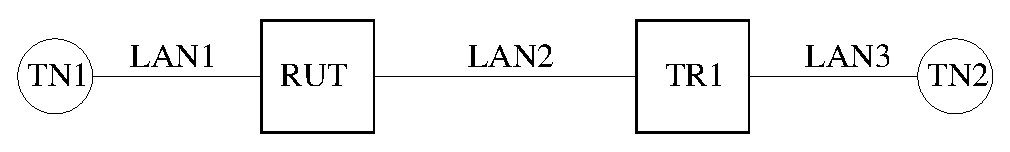
\includegraphics[scale=0.8]{figs/pim_test_1_1_basic_interoperability}
    \caption{Basic interoperability test setup}
    \label{fig:pim_test_1_1_basic_interoperability}
  \end{center}
\end{figure}

\para{Procedure:}

\subpara{Part A: The RUT is the RP, TN1 is the receiver, and TN2 is the
sender.}

Configure both the RUT and TR1 such that the RUT is the RP for group
224.0.1.20. This configuration can be either manual, or implicit through the
Bootstrap mechanism. Configure TN1 and TN2 such that TN1 is the receiver, and
TN2 is the sender, both for group 224.0.1.20.

\begin{enumerate}

  \item Start both the RUT and TR1. If necessary, wait until the RP-set in the
        RUT and TR1 converges.

  \item Start the receiver and the sender.

  \item Observe the data packets received by the receiver.

\end{enumerate}

\subpara{Part B: TR1 is the RP, TN1 is the receiver, and TN2 is the sender.}

Configure both the RUT and TR1 such that TR1 is the RP for group
224.0.1.20. This configuration can be either manual, or implicit through the
Bootstrap mechanism. Configure TN1 and TN2 such that TN1 is the receiver, and
TN2 is the sender, both for group 224.0.1.20. The rest of the procedure is
same as in Part A.

\subpara{Part C: The RUT is the RP, TN2 is the receiver, and TN1 is the
sender.}

Configure both the RUT and TR1 such that the RUT is the RP for group
224.0.1.20. This configuration can be either manual, or implicit through the 
Bootstrap mechanism. Configure TN1 and TN2 such that TN2 is the receiver, and
TN1 is the sender, both for group 224.0.1.20. The rest of the procedure is
same as in Part A.

\subpara{Part D: TR1 is the RP, TN2 is the receiver, and TN1 is the sender.}

Configure both the RUT and TR1 such that TR1 is the RP for group
224.0.1.20. This configuration can be either manual, or implicit through the
Bootstrap mechanism. Configure TN1 and TN2 such that TN2 is the receiver, and
TN1 is the sender, both for group 224.0.1.20. The rest of the procedure is
same as in Part A.

\para{Observable Results:}
In all cases the data packets by the sender should be received by the
receiver.

In Part A, the data packets from TN2 should be encapsulated in PIM Registers
by TR1, unicast to the RUT (the RP), decapsulated by RUT, and then forwarded
(using native multicast) to TN1.
In Part B, the data packets from TN2 should be forwarded by TR1 to the RUT
(using native multicast, because TR1 does not need to encapsulate PIM Registers
to itself), and then forwarded to TN1.
In Part C, the data packets from TN1 should be forwarded (using native
multicast) by the RUT to TR1, and then to TN2.
In Part D, the data packets from TN1 should be encapsulated in PIM Registers
by the RUT, unicast to TN (the RP), decapsulated by TN, and then forwarded
(using native multicast) to TN2.

\para{Possible Problems:}
If the RP-set is empty, or is not same for
the RUT and TR1, no multicast packets will be received by the receiver.

%%%%%%%%%%%%%%%%%%%%%%%%%%%%%%%%%%%%%%%%%%%%%%%%%%%%%%%%%%%%%%%%%%%%%%%
\chapter{Designated Routers (DR) and Hello Messages}

\para{Scope:}
Test PIM router neighbor discovery, option exchange, and DR election.

\para{Overview:}
PIM Hello messages are send periodically on each
PIM-enabled interface. They are used to discover neighboring PIM routers,
to exchange various options, and to elect a Designated Router (DR) per LAN.
Hello messages are also used to provide a keep-alive function to detect a
neighbor loss.

%%%%%%%%%%%%%%%%%%%%%%%%%%%%%%%%%%%%%%%%%%%
\newpage
\section{Hello Transmission}

\para{Purpose:}
Verify that a router properly sends Hello messages.

\para{References:}
\begin{itemize}
  \item draft-ietf-pim-sm-v2-new-05 -- Section 4.3.1
\end{itemize}

\para{Discussion:}
Neighbor discovery of PIM capable routers is accomplished by sending Hello
messages to the ALL-PIM-ROUTERS multicast address (224.0.0.13 for IPv4,
and ``ff02::d'' for IPv6). These Hello messages must contain the following:
\begin{itemize}

  \item The IP TTL MUST be set to one.

  \item The Type field must be set to 0, this designates a PIM Hello message.

\end{itemize}

The router should transmit the Hello messages at an interval of
\verb=Hello_Period= ({\PimsmHelloPeriod}).

\para{Test Setup:}
Connect the RUT according to Figure~\ref{fig:pim_test_2_1_hello_transmission}.
Enable PIM-SM on the RUT.

\begin{figure}[htbp]
  \begin{center}
    
\includegraphics[scale=0.8]{figs/pim_test_2_1_hello_transmission}
    \caption{Hello transmission test setup}
    \label{fig:pim_test_2_1_hello_transmission}
  \end{center}
\end{figure}

\para{Procedure:}
\begin{enumerate}

  \item Start the RUT.

  \item Observe the messages transmitted by the RUT.

\end{enumerate}

\para{Observable Results:}
\begin{itemize}

  \item The RUT should send properly formatted PIM Hello messages to the
        ALL-PIM-ROUTERS multicast address at \verb=Hello_Period=
        ({\PimsmHelloPeriod}) interval.

  \item The first Hello message only should be send after a random
        interval between 0 and \verb=Triggered_Hello_Delay=
        ({\PimsmTriggeredHelloDelay}).

  \item The PIM Hello messages should meet all the requirements in the
        discussion section.

\end{itemize}

\para{Possible Problems:}
None.

%%%%%%%%%%%%%%%%%%%%%%%%%%%%%%%%%%%%%%%%%%%
\newpage
\section{Two-Way Neighbor Adjacency}

\para{Purpose:}
Verify that a router accepts Hello messages and forms a two-way neighbor
adjacency.

\para{References:}
\begin{itemize}
  \item draft-ietf-pim-sm-v2-new-05 -- Section 4.3.1
\end{itemize}

\para{Discussion:}
Neighbor discovery of PIM capable routers is accomplished by sending Hello
messages to the ALL-PIM-ROUTERS address (224.0.0.13 for IPv4,
and ``ff02::d'' for IPv6). As a PIM router receives Hello messages from its
PIM neighbors, it records the neighbor addresses on each interface.

\para{Test Setup:}
Connect the RUT and TR1 according to
Figure~\ref{fig:pim_test_2_2_two_way_neighbor_adjacency}.
Enable PIM-SM on both the RUT and TR1.

\begin{figure}[htbp]
  \begin{center}
    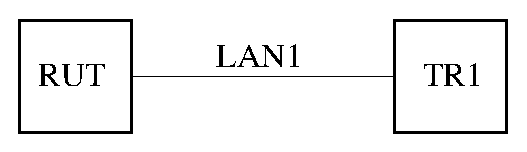
\includegraphics[scale=0.8]{figs/pim_test_2_2_two_way_neighbor_adjacency}
    \caption{Two-way neighbor adjacency test setup}
    \label{fig:pim_test_2_2_two_way_neighbor_adjacency}
  \end{center}
\end{figure}

\para{Procedure:}

\subpara{Part A: Neighbor adjacency when there is network connectivity
failure.}

\begin{enumerate}

  \item Start the RUT.

  \item Observe the neighbor state information in the RUT for at least
        \verb=Triggered_Hello_Delay= ({\PimsmTriggeredHelloDelay}).

  \item Start TR1.

  \item Observe the neighbor state information in the RUT for at least
        \verb=Triggered_Hello_Delay= ({\PimsmTriggeredHelloDelay}).

  \item Disconnect TR1 from LAN1.

  \item Observe the neighbor state information in the RUT for at least
        \verb=Hello_Holdtime= ({\PimsmHelloHoldtime}).

\end{enumerate}

\subpara{Part B: Neighbor adjacency when a neighbor gracefully goes down.}

The procedure is same as in Part A, except that TR1 is gracefully shut-down
instead of disconnected from LAN1.

\subpara{Part C: Neighbor adjacency when the RUT is gracefully shut-down.}

\begin{enumerate}

  \item Start the RUT and TR1.

  \item Observe the neighbor state information in the RUT.

  \item Observe the messages transmitted by the RUT on LAN1.

  \item Gracefully shut-down the RUT.

\end{enumerate}

\para{Observable Results:}

\subpara{Part A:}

\begin{itemize}

  \item Before TR1 is started, the neighbor state information in the RUT should
        show no PIM neighbors:

\begin{verbatim}
Xorp> show pim neighbors 
Interface        DRpriority NeighborAddr    V Mode    Holdtime Timeout
\end{verbatim}

  \item After TR1 is started, and after up to \verb=Triggered_Hello_Delay=
        ({\PimsmTriggeredHelloDelay}), the neighbor state information in the
        RUT must contain TR1:

\begin{verbatim}
Xorp> show pim neighbors 
Interface        DRpriority NeighborAddr     V Mode    Holdtime Timeout
dc1                       1 10.2.0.2         2 Sparse       105     103
\end{verbatim}

  \item After TR1 is disconnected from LAN1, and after up to
        \verb=Hello_Holdtime= ({\PimsmHelloHoldtime}), the neighbor state
        information in the RUT should show no PIM neighbors:

\begin{verbatim}
Xorp> show pim neighbors 
Interface        DRpriority NeighborAddr     V Mode    Holdtime Timeout
\end{verbatim}

\end{itemize}

\subpara{Part B:}

The observed results should be same as in Part A, except that after TR1 is
gracefully shut-down, it would send a Hello message with zero \verb=HoldTime=.
After the RUT receives this Hello message, it should immediately timeout TR1,
instead of up to  \verb=Hello_Holdtime= ({\PimsmHelloHoldtime}).

\subpara{Part C:}

\begin{itemize}

  \item After TR1 is started, and after up to \verb=Triggered_Hello_Delay=
        ({\PimsmTriggeredHelloDelay}), the neighbor state information in the
        RUT must contain TR1:

\begin{verbatim}
Xorp> show pim neighbors 
Interface        DRpriority NeighborAddr     V Mode    Holdtime Timeout
dc1                       1 10.2.0.2         2 Sparse       105     103
\end{verbatim}

  \item Right after the RUT is gracefully shut-down, it should send
        a Hello message with zero \verb=HoldTime=.

\end{itemize}

\para{Possible Problems:}
None.

%%%%%%%%%%%%%%%%%%%%%%%%%%%%%%%%%%%%%%%%%%%
\newpage
\section{Hello Reception}

\para{Purpose:}
Verify that a router properly receives Hello messages.

\para{References:}
\begin{itemize}
  \item draft-ietf-pim-sm-v2-new-05 -- Sections 4.3.1, 4.10, and 4.10.2
\end{itemize}

\para{Discussion:}
Neighbor discovery of PIM capable routers is accomplished by sending Hello
messages to the ALL-PIM-ROUTERS address (224.0.0.13 for IPv4,
and ``ff02::d'' for IPv6). As a PIM router receives Hello messages from its
PIM neighbors, it records the neighbor addresses on each interface.
The checksum is 16-bit one's complement of the one's complement sum of the PIM
messages. The checksum MUST be validated on reception of the message.
The unused and reserved bits MUST be ignored upon reception.

\para{Test Setup:}
Connect the RUT and TR1 according to Figure~\ref{fig:pim_test_2_3_hello_reception}.
Enable PIM-SM on both the RUT and TR1.

\begin{figure}[htbp]
  \begin{center}
    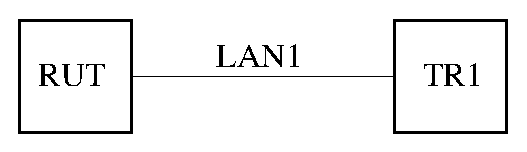
\includegraphics[scale=0.8]{figs/pim_test_2_3_hello_reception}
    \caption{Hello reception test setup}
    \label{fig:pim_test_2_3_hello_reception}
  \end{center}
\end{figure}

\para{Procedure:}

\subpara{Part A: Reception of a PIM Hello message containing an invalid
checksum.}

\begin{enumerate}

  \item TR1 transmits a Hello message with an invalid checksum.

  \item Observe the neighbor state information in the RUT.

\end{enumerate}

\subpara{Part B: Reception of a PIM Hello message containing a Reserved field
of 0xFF.}

\begin{enumerate}

  \item TR1 transmits a Hello message containing a Reserved field of 0xFF.

  \item Observe the neighbor state information in the RUT.

\end{enumerate}

\subpara{Part C: Reception of a PIM Hello message containing a Version field
of 0xF.}

\begin{enumerate}

  \item TR1 transmits a Hello message containing a Version field of 0xF.

  \item Observe the neighbor state information in the RUT.

\end{enumerate}

\subpara{Part D: Reception of a PIM message containing an unrecognized
Type field of 0xF.}

\begin{enumerate}

  \item TR1 transmits a PIM message containing a Type field of 0xF.

  \item Observe the warning log messages in the RUT.

\end{enumerate}

\para{Observable Results:}
\begin{itemize}

  \item In Part A, the Hello messages with invalid checksum should be ignored,
        and the neighbor state information in the RUT should show no PIM
        neighbors:

\begin{verbatim}
Xorp> show pim neighbors 
Interface        DRpriority NeighborAddr     V Mode    Holdtime Timeout
\end{verbatim}


  \item In Part B, after TR1 is started, and after up to
        \verb=Triggered_Hello_Delay=
        ({\PimsmTriggeredHelloDelay}), the neighbor state information in the
        RUT must contain TR1:

\begin{verbatim}
Xorp> show pim neighbors 
Interface        DRpriority NeighborAddr     V Mode    Holdtime Timeout
dc1                       1 10.2.0.2         2 Sparse       105     103
\end{verbatim}

  \item In Part C, after TR1 is started, and after up to
        \verb=Triggered_Hello_Delay=
        ({\PimsmTriggeredHelloDelay}), the neighbor state information in the
        RUT must contain TR1 with protocol version of 15 (0xF).

\begin{verbatim}
Xorp> show pim neighbors 
Interface        DRpriority NeighborAddr     V Mode    Holdtime Timeout
dc2                       1 10.3.0.1        15 Sparse       105     103
\end{verbatim}

  \item In Part D, after TR1 is started and after it sends PIM messages
        containing a Type field of 0xF, the RUT should log the messages with
        this unrecognized Type field:

\begin{verbatim}
[ 2002/08/17 22:45:20 WARNING test_pim.rut PIM ] RX PIM_type_unknown from
10.3.0.2 to 224.0.0.13: message type (15) is unknown
\end{verbatim}

\end{itemize}

\para{Possible Problems:}
\begin{itemize}

  \item Earlier protocol specification (RFC 2117), have ``Addr length''
        field in place of the ``Reserved'' field. Therefore, the test in Part
        B may not be appropriate for such implementations.

  \item At the moment of writing, the lastest
        PIM-SM specification does not describe the behavior if a PIM message is
        received with protocol version that is larger than the implemented
        one.
        (TODO: if the specification later is modified to include that behavior,
        remove this bullet).
        Hence, in Part C, it is possible that an implementation may
        silently ignore all messages with protocol version larger than
        \verb=PIM_SM_version_default= ({\PimsmVersionDefault}).
        As a result, the RUT will not see TR1 as a neighbor.

  \item In Part D, the RUT may not log events such as receiving of a message
        with unrecognized Type field, because the logging is not described
        in the spec.

\end{itemize}

%%%%%%%%%%%%%%%%%%%%%%%%%%%%%%%%%%%%%%%%%%%
\newpage
\section{Holdtime Option}

\para{Purpose:}
Verify that a router properly sends and receives Hello messages with Holdtime
option.

\para{References:}
\begin{itemize}
  \item draft-ietf-pim-sm-v2-new-05 -- Sections 4.3.1 and 4.10.2
\end{itemize}

\para{Discussion:}
PIM capable routers periodically send Hello messages
messages to the ALL-PIM-ROUTERS address (224.0.0.13 for IPv4,
and ``ff02::d'' for IPv6). If a PIM router does not receive a Hello message
from a neighbor for some amount of time, it is assumed that the neighbor (or
the connectivity to it) is not operational, therefore the neighbor is
timed-out. A Hello message may contain a Holdtime option that specifies the
amount of time (in seconds) a router must keep the neighbor reachable.
If a Hello message does not contain a Holdtime option, the default value
of \verb=Default_Hello_Holdtime= ({\PimsmDefaultHelloHoldtime})
is assumed. If a Hello message contains a Holdtime option with value of
0xFFFF, then only one Hello message should be sent, and the router-recipient
of the message should not time-out the router-originator.

\para{Test Setup:}
Connect the RUT and TR1 according to Figure~\ref{fig:pim_test_2_4_holdtime_option}.
Enable PIM-SM on both the RUT and TR1.

\begin{figure}[htbp]
  \begin{center}
    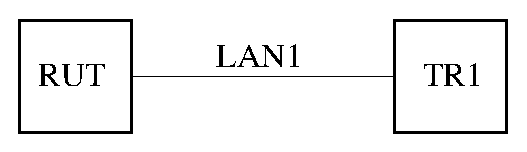
\includegraphics[scale=0.8]{figs/pim_test_2_4_holdtime_option}
    \caption{Holdtime option test setup}
    \label{fig:pim_test_2_4_holdtime_option}
  \end{center}
\end{figure}

\para{Procedure:}

\subpara{Part A: Transmission of a PIM Hello message containing a Holdtime
option.}

\begin{enumerate}

  \item Start the RUT.

  \item Observe the messages transmitted by the RUT for at least
        \verb=Triggered_Hello_Delay= + 3 * \verb=Hello_Holdtime=
        (\ie ({\PimsmTriggeredHelloDelay}) + 3 * ({\PimsmHelloHoldtime})).

  \item Stop the RUT.

  \item Observe the messages transmitted by the RUT for at least
        \verb=Triggered_Hello_Delay= + 3 * \verb=Hello_Holdtime=
        (\ie ({\PimsmTriggeredHelloDelay}) + 3 * ({\PimsmHelloHoldtime})).

  \item Change the configuration value of \verb=Hello_Holdtime= and repeat.

\end{enumerate}

\subpara{Part B: Transmission of a PIM Hello message containing a Holdtime
option with value of 0xFFFF.}

The procedure is same as in Part A, except that the RUT is configured with
Holdtime option value of 0xFFFF. Note that the amount of time to observe the
transmitted messages should be same as in Part A.

\subpara{Part C: Reception of a PIM Hello message containing a Holdtime
option.}

\begin{enumerate}

  \item Start the RUT.

  \item Observe the neighbor state information in the RUT for at least
        \verb=Triggered_Hello_Delay= ({\PimsmTriggeredHelloDelay}).

  \item Configure TR1 such that its Hello messages would contain a Holdtime
        option with the default value of \verb=Hello_Holdtime=
        ({\PimsmHelloHoldtime}).

  \item Start TR1.

  \item Observe the neighbor state information in the RUT for at least
        \verb=Triggered_Hello_Delay= ({\PimsmTriggeredHelloDelay}).

  \item Stop TR1.

  \item Observe the neighbor state information in the RUT for at least
        \verb=Hello_Holdtime= ({\PimsmHelloHoldtime}).

  \item Change the configuration value of \verb=Hello_Holdtime= in TR1 and
        repeat.

\end{enumerate}

\subpara{Part D: Reception of a PIM Hello message containing a Holdtime option
with value of 0xFFFF.}

The procedure is same as in Part C, except that in Step 3 the Hello message
originated by TR1 must be configured contain a Holdtime option with value of
0xFFFF.

\subpara{Part E: Reception of a PIM Hello message that does not contain a
Holdtime option.}

The procedure is same as in Part C, except that in Step 3 the the Hello message
originated by TR1 must be configured to exclude the Holdtime option.

\para{Observable Results:}

\subpara{Part A:}

\begin{itemize}

  \item After the RUT is started, the first Hello message should be
        transmitted no later than \verb=Triggered_Hello_Delay=
        ({\PimsmTriggeredHelloDelay}).

  \item After the first Hello message, there should be one Hello message
        transmitted each \verb=Hello_Period= ({\PimsmHelloPeriod}). Each Hello
        message should contain a Holdtime option with default value of
        \verb=Hello_Holdtime= ({\PimsmHelloHoldtime}).

  \item Right after the RUT is stopped, there should be
        a Hello message transmitted with Holdtime option value of 0.

  \item After the Hello message with Holdtime option value of 0,
        no other Hello messages should be transmitted.

  \item The results of repeating the test with different value of
        \verb=Hello_Holdtime= should be similar, except that the
        Hello messages should be transmitted every 1/3th of
        the new \verb=Hello_Holdtime=, and the Holdtime Option value
        in the Hello messages should be the new \verb=Hello_Holdtime=.

\end{itemize}

\subpara{Part B:}

\begin{itemize}

  \item After the RUT is started, the first Hello message should be
        transmitted no later than \verb=Triggered_Hello_Delay=
        ({\PimsmTriggeredHelloDelay}). This message should contain
        a Holdtime option with value of 0xFFFF.

  \item After the first Hello message, there should be no one Hello messages
        transmitted before the RUT is stopped.

  \item Right after the RUT is stopped, there should be
        a Hello message transmitted with Holdtime option value of 0.

  \item After the Hello message with Holdtime option value of 0,
        no other Hello messages should be transmitted.

\end{itemize}

\subpara{Part C:}

\begin{itemize}

  \item Before TR1 is started, the neighbor state information in the RUT
  should show no PIM neighbors:

\begin{verbatim}
Xorp> show pim neighbors
Interface        DRpriority NeighborAddr    V Mode    Holdtime Timeout
\end{verbatim}

  \item After TR1 is started, and after up to \verb=Triggered_Hello_Delay=
        ({\PimsmTriggeredHelloDelay}), the neighbor state information in the
        RUT must contain TR1. The Holdtime information about TR1 must match
        the Holdtime value in the Hello messages by TR1:

\begin{verbatim}
Xorp> show pim neighbors
Interface        DRpriority NeighborAddr     V Mode    Holdtime Timeout
dc1                       1 10.2.0.2         2 Sparse       105     103
\end{verbatim}

  \item After TR1 is stopped, and after it sends a Hello message with Holdtime
        option value of 0, the RUT must immediately expire it.
        The neighbor state information in the RUT should show no PIM
        neighbors:

\begin{verbatim}
Xorp> show pim neighbors
Interface        DRpriority NeighborAddr     V Mode    Holdtime Timeout
\end{verbatim}

  \item The results of repeating the test with different value of
        \verb=Hello_Holdtime= should be similar, except that the
        Holdtime value in the state information in the RUT about TR1 should
        match the chosen value of the \verb=Hello_Holdtime=.

\end{itemize}

\subpara{Part D:}

The observed results should be same as in Part C, except that
after the first Hello message from TR1 is received, the neighbor state
information in the RUT must show that the TR1 would never be expired:

\begin{verbatim}
Xorp> show pim neighbors 
Interface        DRpriority NeighborAddr     V Mode    Holdtime Timeout
dc1                       1 10.3.0.2         2 Sparse     65535    None
\end{verbatim}

\subpara{Part E:}

The observed results should be same as in Part C, except that
the RUT assumes that the Holdtime value about TR1 is always equal to the
default value of \verb=Hello_Holdtime= ({\PimsmHelloHoldtime}).

\para{Possible Problems:}
None.

%%%%%%%%%%%%%%%%%%%%%%%%%%%%%%%%%%%%%%%%%%%
\newpage
\section{DR Priority Option}

\para{Purpose:}
Verify that a router properly sends and receives Hello messages with DR
Priority option.

\para{References:}
\begin{itemize}
  \item draft-ietf-pim-sm-v2-new-05 -- Sections 4.3.1, 4.3.2, and 4.10.2
\end{itemize}

\para{Discussion:}
One of the PIM routers on each LAN, the Designated Router (DR), needs to act
on behalf of the rest of the routers and directly connected hosts with respect
to the PIM protocol. The DR election considers the DR priority of each
PIM router and its IP address: numerically larger DR priority is always
better, with a numerically larger IP address used as a tie-break. Each PIM
router includes its DR priority in the DR Priority option of the Hello
messages it originates. If there is at least one PIM router on a LAN that does
not include the DR Priority option in its Hello messages, then the DR election
process considers only the IP addresses of the routers.

\para{Test Setup:}
Connect the RUT and TR1 according to Figure~\ref{fig:pim_test_2_5_dr_priority_option}.
Enable PIM-SM on both the RUT and TR1.

\begin{figure}[htbp]
  \begin{center}
    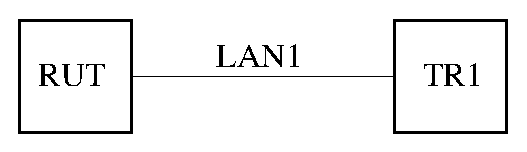
\includegraphics[scale=0.8]{figs/pim_test_2_5_dr_priority_option}
    \caption{DR priority option test setup}
    \label{fig:pim_test_2_5_dr_priority_option}
  \end{center}
\end{figure}

\para{Procedure:}

\subpara{Part A: The RUT has a numerically larger IP address than TR1.}

\begin{enumerate}

  \item Start the RUT with default DR priority of 1, and
        observe the DR state information in the RUT.

  \item Start TR1 with default DR priority of 1, and
        observe the DR state information in the RUT.

  \item Change the DR priority of TR1 to 2, and
        observe the DR state information in the RUT.

  \item Change the DR priority of TR1 to 0, and
        observe the DR state information in the RUT.

  \item Change the DR priority of TR1 to 1, and
        observe the DR state information in the RUT.

  \item Change the DR priority of the RUT to 2, and
        observe the DR state information in the RUT.

  \item Change the DR priority of the RUT to 0, and
        observe the DR state information in the RUT.

  \item Change the DR priority of the RUT to 1, and
        observe the DR state information in the RUT.

\end{enumerate}

\subpara{Part B: The RUT has a numerically smaller IP address than TR1.}

The procedure is same as in Part A, except that TR1 has a numerically smaller
IP address than TR1.

\para{Observable Results:}

\subpara{Part A:}

\begin{enumerate}

  \item After the RUT is started with default DR priority of 1, it should
        be the DR for LAN1:

\begin{verbatim}
Xorp> show pim interface dc2
Interface       State    Mode    V PIMstate  Priority DRaddr      Neighbors
dc2             UP       Sparse  2 DR               1 10.2.0.2            0
\end{verbatim}

  \item After TR1 is started with default DR priority of 1, the RUT should be
        still the DR for LAN1:

\begin{verbatim}
Xorp> show pim interface dc2
Interface       State    Mode    V PIMstate  Priority DRaddr      Neighbors
dc2             UP       Sparse  2 DR               1 10.2.0.2            1
\end{verbatim}

  \item After the DR priority of TR1 is increased to 2, TR1 should become the
  DR for LAN1. The DR state information in the RUT should show that the RUT is
  not the DR anymore:

\begin{verbatim}
Xorp> show pim interface dc2
Interface       State    Mode    V PIMstate  Priority DRaddr      Neighbors
dc2             UP       Sparse  2 NotDR            1 10.2.0.1            1
\end{verbatim}

  \item After the DR priority of TR1 is decreased to 0, the RUT should become
        the DR for LAN1:

\begin{verbatim}
Xorp> show pim interface dc2
Interface       State    Mode    V PIMstate  Priority DRaddr      Neighbors
dc2             UP       Sparse  2 DR               1 10.2.0.2            1
\end{verbatim}

  \item After the DR priority of TR1 is increased to 1, the RUT should
        continue to be the DR for LAN1: 

\begin{verbatim}
Xorp> show pim interface dc2
Interface       State    Mode    V PIMstate  Priority DRaddr      Neighbors
dc2             UP       Sparse  2 DR               1 10.2.0.2            1
\end{verbatim}

  \item After the DR priority of the RUT is increased to 2, the RUT should
        continue to be the DR for LAN1:

\begin{verbatim}
Xorp> show pim interface dc2
Interface       State    Mode    V PIMstate  Priority DRaddr     Neighbors
dc2             UP       Sparse  2 DR               2 10.2.0.2           1
\end{verbatim}

  \item After the DR priority of the RUT is decreased to 0, TR1 should become
        the DR for LAN1. The DR state information in the RUT should show that
        the RUT is not the DR anymore:

\begin{verbatim}
Xorp> show pim interface dc2
Interface       State    Mode    V PIMstate  Priority DRaddr     Neighbors
dc2             UP       Sparse  2 NotDR            0 10.2.0.1           1
\end{verbatim}

  \item After the DR priority of the RUT is increased to 1, the RUT should
        become the DR for LAN1:

\begin{verbatim}
Xorp> show pim interface dc2
Interface       State    Mode    V PIMstate  Priority DRaddr      Neighbors
dc2             UP       Sparse  2 DR               1 10.2.0.2            1
\end{verbatim}

\end{enumerate}

\subpara{Part B:}

\begin{enumerate}

  \item After the RUT is started with default DR priority of 1, it should
        be the DR for LAN1:

\begin{verbatim}
Xorp> show pim interface dc2
Interface       State    Mode    V PIMstate  Priority DRaddr      Neighbors
dc2             UP       Sparse  2 DR               1 10.2.0.2            0
\end{verbatim}

  \item After TR1 is started with default DR priority of 1, it should become
        the DR for LAN1. The DR state information in the RUT should show that
        the RUT is not the DR anymore:

\begin{verbatim}
Xorp> show pim interface dc2
Interface       State    Mode    V PIMstate  Priority DRaddr      Neighbors
dc2             UP       Sparse  2 NotDR            1 10.2.0.3            1
\end{verbatim}

  \item After the DR priority of TR1 is increased to 2, TR1 should continue to
        be the DR for LAN1. The DR state information in the RUT should show
        that the RUT is not the DR:

\begin{verbatim}
Xorp> show pim interface dc2
Interface       State    Mode    V PIMstate  Priority DRaddr      Neighbors
dc2             UP       Sparse  2 NotDR            1 10.2.0.3            1
\end{verbatim}

  \item After the DR priority of TR1 is decreased to 0, the RUT should become
        the DR for LAN1:

\begin{verbatim}
Xorp> show pim interface dc2
Interface       State    Mode    V PIMstate  Priority DRaddr      Neighbors
dc2             UP       Sparse  2 DR               1 10.2.0.2            1
\end{verbatim}

  \item After the DR priority of TR1 is increased to 1, TR1 should become the
        DR for LAN1. The DR state in the RUT should show that the RUT is not
        the DR:

\begin{verbatim}
Xorp> show pim interface dc2
Interface       State    Mode    V PIMstate  Priority DRaddr      Neighbors
dc2             UP       Sparse  2 NotDR            1 10.2.0.3            1
\end{verbatim}

  \item After the DR priority of the RUT is increased to 2, the RUT should
        become the DR for LAN1:

\begin{verbatim}
Xorp> show pim interface dc2
Interface       State    Mode    V PIMstate  Priority DRaddr      Neighbors
dc2             UP       Sparse  2 DR               2 10.2.0.2            1
\end{verbatim}

  \item After the DR priority of the RUT is decreased to 0, TR1 should become
        the DR for LAN1. The DR state in the RUT should show that the RUT
        is not the DR:

\begin{verbatim}
Xorp> show pim interface dc2
Interface       State    Mode    V PIMstate  Priority DRaddr      Neighbors
dc2             UP       Sparse  2 NotDR            0 10.2.0.3            1
\end{verbatim}

  \item After the DR priority of the RUT is increased to 1, TR1 should
        continue to be the DR for LAN1. The DR state information in the RUT
        should show that the RUT is not the DR:

\begin{verbatim}
Xorp> show pim interface dc2
Interface       State    Mode    V PIMstate  Priority DRaddr      Neighbors
dc2             UP       Sparse  2 NotDR            1 10.2.0.3            1
\end{verbatim}

\end{enumerate}

\para{Possible Problems:}
None.

%%%%%%%%%%%%%%%%%%%%%%%%%%%%%%%%%%%%%%%%%%%
\newpage
\section{Generation ID Option}

\para{Purpose:}
Verify that a router properly sends and receives Hello messages with
Generation ID option.

\para{References:}
\begin{itemize}
  \item draft-ietf-pim-sm-v2-new-05 -- Sections 4.3.1 and 4.10.2
\end{itemize}

\para{Discussion:}
The Generation ID (GenID) option contains a randomly generated 32-bit value
that is regenerated each time PIM forwarding is started or restarted on the
interface, including when the router itself restarts. When a Hello message
with a new GenID is received from a neighbor, any old Hello information about
that neighbor should be discarded and superseded by the information from the
new Hello message. In addition, if a router needs to send a Join/Prune or some
other control messages to the new neighbor, then it must send a Hello
message, immediately followed by the relevant control messages.

\para{Test Setup:}
Connect the RUT, TR1, and Rx1 according to
Figure~\ref{fig:pim_test_2_6_generation_id_option}.
Enable PIM-SM on both the RUT and TR1.

\begin{figure}[htbp]
  \begin{center}
    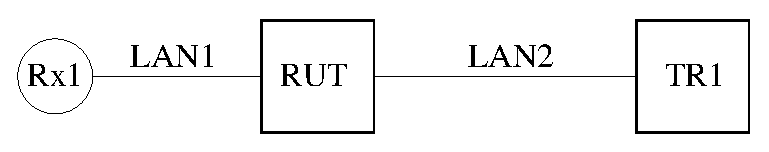
\includegraphics[scale=0.8]{figs/pim_test_2_6_generation_id_option}
    \caption{Generation ID option test setup}
    \label{fig:pim_test_2_6_generation_id_option}
  \end{center}
\end{figure}

\para{Procedure:}

\subpara{Part A: Transmission of a PIM Hello message containing a Generation ID
option.}

\begin{enumerate}

  \item Start the RUT.

  \item Observe the messages transmitted by the RUT on LAN2 for at least
        \verb=Triggered_Hello_Delay= + 3 * \verb=Hello_Holdtime=
        (\ie ({\PimsmTriggeredHelloDelay}) + 3 * ({\PimsmHelloHoldtime})).

  \item Restart the RUT interface that connects the RUT to LAN2.

  \item Observe the messages transmitted by the RUT on LAN2 for at least
        \verb=Triggered_Hello_Delay= ({\PimsmTriggeredHelloDelay}).

  \item Restart the RUT.

  \item Observe the messages transmitted by the RUT on LAN2 for at least
        \verb=Triggered_Hello_Delay= ({\PimsmTriggeredHelloDelay}).

\end{enumerate}

\subpara{Part B: Reception of a PIM Hello message containing a Generation ID
option.}

\begin{enumerate}

  \item Start both the RUT and TR1.

  \item Observe the messages transmitted by the RUT on LAN2.

  \item Quit TR1 (\ie stop it without graceful shutdown), and start it
  immediately.

\end{enumerate}

\subpara{Part C: Reception of a PIM Hello message containing a Generation ID
option when the RUT has pending Join messages to send.}

Configure both the RUT and TR1 such that it is the RP for group
224.0.1.20. This configuration can be either manual, or implicit through the
Bootstrap mechanism. Configure Rx1 such that it is the receiver for group
224.0.1.20.

\begin{enumerate}

  \item Start both the RUT and TR1. If necessary, wait until the RP-set in the
  RUT and TR1 converges.

  \item Start Rx1, and observe the Join state in the RUT and TR1.

  \item Observe the messages transmitted by the RUT on LAN2.

  \item Quit TR1 (\ie stop it without graceful shutdown), and start it
  immediately.

\end{enumerate}

\para{Observable Results:}

\subpara{Part A:}

\begin{itemize}

  \item After the RUT is started, after a random interval between
        0 and \verb=Triggered_Hello_Delay= ({\PimsmTriggeredHelloDelay}) the
        RUT should start transmitting Hello message with Generation ID
        option included. There should be a Hello message every
        \verb=Hello_Holdtime= ({\PimsmHelloHoldtime}), and the value of the
        Generation ID must be same for all messages.

  \item After the RUT interface that connects the RUT to LAN2 is restarted,
        after a random interval between 0 and \verb=Triggered_Hello_Delay=
        ({\PimsmTriggeredHelloDelay}) the RUT should transmit on LAN2 a Hello
        message with Generation ID option included. The value of this
        Generation ID must be different from the value of the Hello message
        before the restart.

  \item After the RUT is restarted,
        after a random interval between 0 and \verb=Triggered_Hello_Delay=
        ({\PimsmTriggeredHelloDelay}) the RUT should transmit on LAN2 a Hello
        message with Generation ID option included. The value of this
        Generation ID must be different from the value of the Hello message
        before the restart.
        
\end{itemize}

\subpara{Part B:}

\begin{itemize}

  \item After the RUT receives the first Hello message from TR1 that
	has different Generation ID from the one before the restart,
        after a random interval between 0 and \verb=Triggered_Hello_Delay=
        ({\PimsmTriggeredHelloDelay}) the RUT should transmit on LAN2 a Hello
        message.

\end{itemize}

\subpara{Part C:}

\begin{itemize}

  \item After the RUT receives the first Hello message from TR1 that
	has different Generation ID from the one before the restart,
	the RUT should transmit immediately on LAN2 a Hello message
	followed by a PIM Join/Prune message with group 224.0.1.20
	included in the list of joined groups.

\end{itemize}

\para{Possible Problems:}
None.

%%%%%%%%%%%%%%%%%%%%%%%%%%%%%%%%%%%%%%%%%%%
\newpage
\section{Two-Way Neighbor Adjacency Without Hello Messages}

\para{Purpose:}
Verify that a router can be configured to form a two-way neighbor adjacency
even if no Hello message was received.

\para{References:}
\begin{itemize}
  \item draft-ietf-pim-sm-v2-new-05 -- Sections 4.3.1, and 4.5
  \item draft-ietf-pim-sm-bsr-03 -- Section 3
\end{itemize}

\para{Discussion:}
The following PIM control messages should only be accepted for processing if
they come from a known PIM neighbor: Join/Prune, Bootstrap, Assert, Graft, and
Graft-Ack. A PIM router hears about PIM neighbors
through PIM Hello messages. However, some older PIM implementations
incorrectly fail to send Hello messages on point-to-point interfaces. Hence,
the protocol specification recommends that a configuration option should be
provided to allow 
interoperation with such old routers (disabled by default). More specifically,
if the option is enabled, then the above PIM control messages should be
accepted from a neighbor even if no Hello message was received first from that
neighbor.

\para{Test Setup:}
Connect the RUT, TR1, S1, and Rx1 according to
Figure~\ref{fig:pim_test_2_7_two_way_neighbor_adjacency_without_hello_messages}.
Enable PIM-SM on both TR1 and the RUT. Configure TR1
as a Candidate-BSR, and the RUT as a Candidate-RP. Modify or configure TR1
such that it never sends PIM Hello messages. Configure Rx1 and S1 such
that Rx1 is a receiver, and S1 is a sender, both for group 224.0.1.20.

\begin{figure}[htbp]
  \begin{center}
    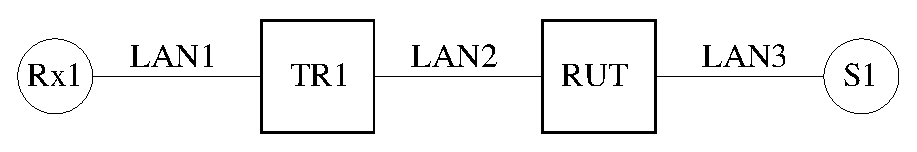
\includegraphics[scale=0.8]{figs/pim_test_2_7_two_way_neighbor_adjacency_without_hello_messages}
    \caption{Two-way neighbor adjacency without Hello messages test
    setup}
    \label{fig:pim_test_2_7_two_way_neighbor_adjacency_without_hello_messages}
  \end{center}
\end{figure}

\para{Procedure:}

\begin{enumerate}

  \item Start TR1 and the RUT.

  \item Observe the messages transmitted by TR1 and the RUT, and the neighbor
  and Bootstrap state information in the RUT.

  \item Wait until TR1 transmits 2-3 Bootstrap messages.

  \item Enable the interoperability option in the RUT (without restarting it),
  such that the RUT would accept PIM control messages from TR1 even if TR1
  does not send Hello messages.

  \item Wait until TR1 transmits 2-3 Bootstrap messages.

  \item Start Rx1.

  \item Start S1.

\end{enumerate}

\para{Observable Results:}

\begin{itemize}

  \item After TR1 and the RUT are started, the RUT should start transmitting
  PIM Hello messages on LAN2.

  \item After TR1 receives the first Hello message from the RUT, TR1 should
  unicast a Bootstrap message to the RUT. After that it start transmitting
  periodically only Bootstrap messages on LAN2.

  \item Each Bootstrap message received by the RUT should be ignored because
  it comes from an unknown neighbor. Therefore, the RUT should not have a
  BSR:

\begin{verbatim}
Xorp> show pim bootstrap
Active zones:
BSR              Pri LocalAddress     Pri State            Timeout SZTimeout
Expiring zones:
BSR              Pri LocalAddress     Pri State            Timeout SZTimeout
Configured zones:
BSR              Pri LocalAddress     Pri State            Timeout SZTimeout
0.0.0.0            0 0.0.0.0            0 Init                  -1        -1
\end{verbatim}

  In addition, the neighbor state information in the RUT should be empty:

\begin{verbatim}
Xorp> show pim neighbors 
Interface        DRpriority NeighborAddr     V Mode    Holdtime Timeout
\end{verbatim}


  \item After the interoperability option in the RUT is enabled, the next
  Bootstrap message from TR1 should be accepted by the RUT. As a result, the
  Bootstrap state in the RUT should show that TR1 is the BSR:

\begin{verbatim}
Xorp> show pim bootstrap
Active zones:
BSR              Pri LocalAddress     Pri State            Timeout SZTimeout
10.2.0.1           1 0.0.0.0            0 AcceptPreferred       74      1444
\end{verbatim}

  Eventually, the neighbor state information in the RUT may show TR1. If this
  is the case, the state information in the RUT for TR1 should be refreshed by
  each Bootstrap originated by TR1:

\begin{verbatim}
Xorp> show pim neighbors 
Interface        DRpriority NeighborAddr     V Mode    Holdtime Timeout
dc2                    none 10.2.0.1         2 Sparse       210     164
\end{verbatim}

  \item After Rx1 is started, TR1 should send PIM Join message for group
  224.0.1.20 on LAN2 toward the RP (the RUT).

  \item After S1 is started, the multicast data packets originated by it
  should be forwarded by the RUT and TR1 to Rx1.

\end{itemize}

\para{Possible Problems:}
None.


%%%%%%%%%%%%%%%%%%%%%%%%%%%%%%%%%%%%%%%%%%%%%%%%%%%%%%%%%%%%%%%%%%%%%%%
\chapter{PIM Register Messages}

\para{Scope:}
Test sending and receiving of PIM Register messages.

\para{Overview:}
The Designated Router (DR) on a LAN or point-to-point link encapsulates
multicast packets from local sources to the RP for the relevant group
unless it recently received a Register-Stop message for that (S,G) or
(*,G) from the RP.  When the DR receives a Register-Stop message from
the RP, it starts a Register-Stop Timer to maintain this state.  Just
before the Register-Stop Timer expires, the DR sends a Null-Register
message to the RP to allow the RP to refresh the Register-Stop
information at the DR.  If the Register-Stop Timer actually expires, the
DR will resume encapsulating packets from the source to the RP.

%%%%%%%%%%%%%%%%%%%%%%%%%%%%%%%%%%%%%%%%%%%
\newpage
\section{Register Messages Transmission}

\para{Purpose:}
Verify that a DR properly sends Register messages.

\para{References:}
\begin{itemize}
  \item draft-ietf-pim-sm-v2-new-05 -- Section 4.4.1
\end{itemize}

\para{Discussion:}
The DR encapsulates multicast packets from local sources into PIM Register
messages, and unicasts them to the RP for the relevant multicast group.

\para{Test Setup:}
Connect the RUT, TR1, TR2, S1, and Rx1 according to
Figure~\ref{fig:pim_test_3_1_register_messages_transmission}.
Configure the RUT, TR1, and TR2 such that TR1 is the RP for group 224.0.1.20,
and such that it never attempts to switch to the shortest-path tree by
originating an (S,G) SPT Join message toward a source.
Enable PIM-SM on the RUT, TR1, and TR2.
Configure Rx1 and S1 such that Rx1 is a receiver, and S1 is a sender,
both for group 224.0.1.20.


\begin{figure}[htbp]
  \begin{center}
    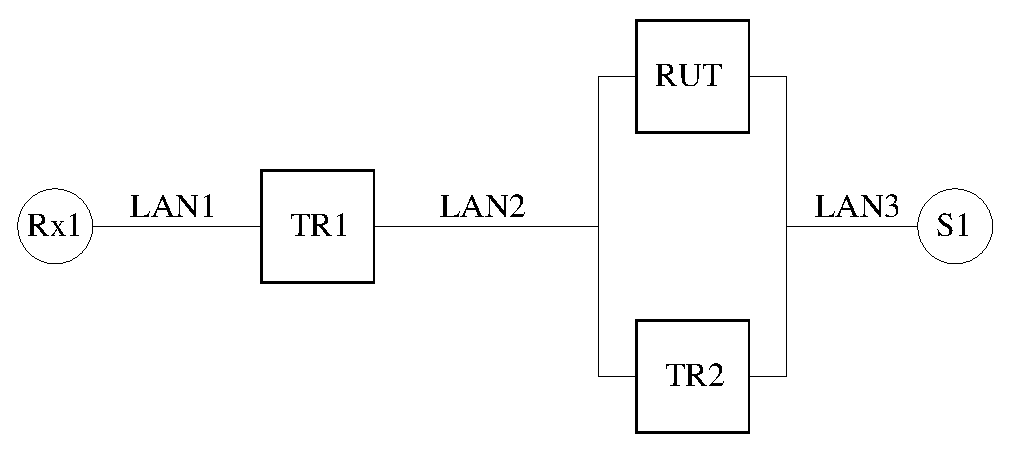
\includegraphics[scale=0.8]{figs/pim_test_3_1_register_messages_transmission}
    \caption{Register messages transmission test setup}
    \label{fig:pim_test_3_1_register_messages_transmission}
  \end{center}
\end{figure}

\para{Procedure:}

\subpara{Part A: Transmission of Register messages.}

\begin{enumerate}

  \item Configure the RUT such that it is the DR on LAN3.

  \item Start the RUT, TR1, and TR2. If necessary, wait until the RP-set in
        the RUT, TR1, and TR1 converges.

  \item Start Rx1.

  \item Observe the messages transmitted by the RUT and TR2 on LAN2.

  \item Start S1.

\end{enumerate}

\subpara{Part B: Non-transmission of Register messages.}

The procedure is same as in Part A, except that TR1 instead of the RUT is the
DR on LAN3.

\subpara{Part C: Switching between transmission and non-transmission of
Register messages.}

\begin{enumerate}

  \item Configure the RUT such that it is the DR on LAN3.

  \item Start the RUT, TR1, and TR2. If necessary, wait until the RP-set in
        the RUT, TR1, and TR1 converges.

  \item Start Rx1.

  \item Observe the messages transmitted by the RUT and TR2 on LAN2.

  \item Start S1.

  \item Reconfigure the RUT (without stopping it), such that TR2 is the DR on
  LAN3.

  \item Reconfigure the RUT (without stopping it), such that it again is the
  DR on LAN3.

\end{enumerate}

\subpara{Part D: Handling of Register-Stop(S,G) messages at the DR.}

\begin{enumerate}

  \item Start the RUT and TR1 (note that in this part we do not use TR2). If
  necessary, wait until the RP-set in the RUT and TR1 converges.

  \item Start Rx1.

  \item Observe the messages transmitted by the RUT on LAN2.

  \item Start S1.

  \item Stop Rx1.

  \item Start Rx1.

\end{enumerate}

\para{Observable Results:}

\subpara{Part A:}

After S1 is started, the RUT should start encapsulating
the data packets transmitted by S1 in PIM Register messages, and unicast them
to the RP (TR1, that should decapsulate and forward them to Rx1).

\subpara{Part B:}

After S1 is started, the RUT should NOT encapsulate the
data packets transmitted by S1 in PIM Register messages. Instead, TR2 should
encapsulate and unicast them to the RP (TR1, that should decapsulate and
forward them to Rx1).

\subpara{Part C:}

\begin{itemize}

  \item After S1 is started, the RUT should start
  encapsulating the data packets transmitted by S1 in PIM Register messages,
  and unicast them to the RP (TR1, that should decapsulate and forward them to
  Rx1).

  \item After the RUT is reconfigured such that it is not the DR on LAN3, it
  should immediately stop transmitting PIM Register messages to the RP.
  Instead, the new DR (TR2) should start transmitting them.

  \item After the RUT is reconfigured such that it is again the DR on LAN3, it
  should immediately start transmitting PIM Register messages to the RP.
  The previous DR (TR2) should stop transmitting them.

\end{itemize}

\subpara{Part D:}

\begin{itemize}

  \item After S1 is started, the RUT should start
  encapsulating the data packets transmitted by S1 in PIM Register messages,
  and unicast them to the RP (TR1, that should decapsulate and forward them to
  Rx1).

  \item After Rx1 is stopped, TR1 should send PIM Register-Stop message to
  the RUT for each PIM Register message it receives from the RUT (including
  the PIM Null-Register messages). After receiving the first PIM Register-Stop
  message, the RUT should stop sending PIM Register messages to the RP (TR1)
  with the encapsulated data packets from S1.
  However, from time to time the RUT should be sending PIM Null-Register
  messages to the RP (TR1) with time interval between two messages a random
  value chosen uniformly from the interval \\
  (0.5 * \verb=Register_Suppression_Time=,
  1.5 * \verb=Register_Suppression_Time=) \\
  - \verb=Register_Probe_Time= \\
  = ( (0.5 * {\PimsmRegisterSuppressionTime}, 1.5 *
  {\PimsmRegisterSuppressionTime}) - {\PimsmRegisterProbeTime} ). \\
  To each PIM Null-Register message, the RP (TR1) should respond with a PIM
  Register-Stop message, therefore the RUT should continue not to encapsulate
  the data packets from S1.

  \item After Rx1 is started again, the RP (TR1) should send an SPT (S,G) Join
  message on LAN2 toward the source. As a result, the data packets from S1
  should be forwarded to the RP (TR1) natively instead of encapsulating them
  in PIM Register messages.

\end{itemize}


\para{Possible Problems:}
In Part C, if the sender's rate is relatively high, there could be few packet
losses at Rx1 when the DR on LAN3 changes.

%%%%%%%%%%%%%%%%%%%%%%%%%%%%%%%%%%%%%%%%%%%
\newpage
\section{Register Tunnel Interface}

\para{Purpose:}
Verify that a Register tunnel virtual interface is properly created, removed,
or changed.

\para{References:}
\begin{itemize}
  \item draft-ietf-pim-sm-v2-new-05 -- Section 4.4.1
\end{itemize}

\para{Discussion:}
When the DR has to encapsulate the data packets from local sources into
PIM Register messages, and unicasts them to the RP for the relevant multicast
group, it creates a Register tunnel virtual interface with its encapsulation
target being the RP. If the DR should stop encapsulating the data packets, it
removes the Register tunnel virtual interface. If the RP for the multicast
group changes, the DR should update the Register tunnel virtual interface.

\para{Test Setup:}
Connect the RUT, TR1, TR2, S1, and Rx1 according to
Figure~\ref{fig:pim_test_3_2_register_tunnel_interface}.
Enable PIM-SM on the RUT, TR1,
and TR2. In all the tests, configure the RP such that it never attempts to
switch to the shortest-path tree by originating an (S,G) SPT Join message
toward a source. Enable PIM-SM on the RUT, TR1, and TR2.  Configure Rx1 and S1
such that Rx1 is a receiver, and S1 is a sender, both for group 224.0.1.20.


\begin{figure}[htbp]
  \begin{center}
    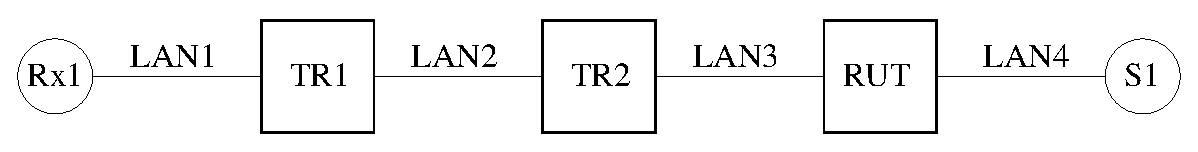
\includegraphics[scale=0.8]{figs/pim_test_3_2_register_tunnel_interface}
    \caption{Register tunnel interface test setup}
    \label{fig:pim_test_3_2_register_tunnel_interface}
  \end{center}
\end{figure}

\para{Procedure:}

\subpara{Part A: Add and remove Register tunnel.}

\begin{enumerate}

  \item Configure TR1 such that it is the RP.

  \item Start the RUT, TR1, and TR2. If necessary, wait until the RP-set in
  the RUT, TR1, and TR2 converges.

  \item Start Rx1.

  \item Observe the Register state machine at the RUT, and the messages
  transmitted by the RUT on LAN3.

  \item Start S1.

  \item Stop Rx1.

  \item Stop S1.

\end{enumerate}

\subpara{Part B: Update Register tunnel.}

\begin{enumerate}

  \item Configure TR1 such that it is the RP.

  \item Start the RUT, TR1, and TR2. If necessary, wait until the RP-set in
  the RUT, TR1, and TR2 converges.

  \item Start Rx1.

  \item Observe the Register state machine at the RUT, and the messages
  transmitted by the RUT on LAN3.

  \item Start S1.

  \item Reconfigure TR1 and TR2 such that TR2 becomes the RP.

\end{enumerate}

\para{Observable Results:}

\subpara{Part A:}

\begin{itemize}

  \item After Rx1 is started, the Register state machine in the RUT for source
  S1 and group 224.0.1.20 should be in No Info state:

\begin{verbatim}
Xorp> show pim join 224.0.1.20
Group           Source          RP              Flags
\end{verbatim}

  Further, no PIM Register messages should be transmitted by the RUT.

  \item After S1 is started, the Register state machine in the RUT for source
  S1 and group 224.0.1.20 should be in Join state, and the Register tunnel
  virtual interface should be created between the RUT and the RP (TR1):

\begin{verbatim}
Xorp> show pim join 224.0.1.20
Group           Source          RP              Flags
224.0.1.20      10.4.0.2        10.2.0.1        SG SPT DirectlyConnectedS 
    Upstream interface (S):    dc0
    Upstream interface (RP):   dc2
    Upstream MRIB next hop (RP): 10.3.0.1
    Upstream MRIB next hop (S):  UNKNOWN
    Upstream RPF'(S,G):        UNKNOWN
    Upstream state:            Joined 
    Register state:            RegisterJoin RegisterCouldRegister 
    Join timer:                13
    Local receiver include WC: .............
    Local receiver include SG: .............
    Local receiver exclude SG: .............
    Joins RP:                  .............
    Joins WC:                  .............
    Joins SG:                  ............O
    Join state:                ............O
    Prune state:               .............
    Prune pending state:       .............
    I am assert winner state:  .............
    I am assert loser state:   .............
    Assert winner WC:          .............
    Assert winner SG:          .............
    Assert lost WC:            .............
    Assert lost SG:            .............
    Assert lost SG_RPT:        .............
    Assert tracking SG:        ....O.......O
    Could assert WC:           .............
    Could assert SG:           ............O
    I am DR:                   ....O.O......
    Immediate olist RP:        .............
    Immediate olist WC:        .............
    Immediate olist SG:        ............O
    Inherited olist SG:        ............O
    Inherited olist SG_RPT:    .............
    PIM include WC:            .............
    PIM include SG:            .............
    PIM exclude SG:            .............
\end{verbatim}

  Further, each data packet from S1 should be encapsulated by the RUT in a
  PIM Register message and unicast to the RP (TR1).

  \item After Rx1 is stopped, the RP (TR1) should send PIM Register-Stop
  message to the RUT for each PIM Register message it receives from the RUT
  (PIM Null-Register messages excluded). After the RUT receives the first
  PIM Register-Stop message, the Register tunnel virtual interface to the RP
  (TR1) should be in Prune state:

\begin{verbatim}
Xorp> show pim join 224.0.1.20
Group           Source          RP              Flags
224.0.1.20      10.4.0.2        10.2.0.1        SG DirectlyConnectedS 
    Upstream interface (S):    dc0
    Upstream interface (RP):   dc2
    Upstream MRIB next hop (RP): 10.3.0.1
    Upstream MRIB next hop (S):  UNKNOWN
    Upstream RPF'(S,G):        UNKNOWN
    Upstream state:            NotJoined 
    Register state:            RegisterPrune RegisterCouldRegister 
    Join timer:                -1
    Local receiver include WC: .............
    Local receiver include SG: .............
    Local receiver exclude SG: .............
    Joins RP:                  .............
    Joins WC:                  .............
    Joins SG:                  .............
    Join state:                .............
    Prune state:               .............
    Prune pending state:       .............
    I am assert winner state:  .............
    I am assert loser state:   .............
    Assert winner WC:          .............
    Assert winner SG:          .............
    Assert lost WC:            .............
    Assert lost SG:            .............
    Assert lost SG_RPT:        .............
    Assert tracking SG:        .............
    Could assert WC:           .............
    Could assert SG:           .............
    I am DR:                   ....O.O......
    Immediate olist RP:        .............
    Immediate olist WC:        .............
    Immediate olist SG:        .............
    Inherited olist SG:        .............
    Inherited olist SG_RPT:    .............
    PIM include WC:            .............
    PIM include SG:            .............
    PIM exclude SG:            .............
\end{verbatim}

  Further, from time to time the RUT should be sending PIM Null-Register
  messages to the RP (TR1) with time interval between two messages a random
  value chosen uniformly from the interval \\
  (0.5 * \verb=Register_Suppression_Time=,
  1.5 * \verb=Register_Suppression_Time=) \\
  - \verb=Register_Probe_Time= \\
  = ( (0.5 * {\PimsmRegisterSuppressionTime}, 1.5 *
  {\PimsmRegisterSuppressionTime}) - {\PimsmRegisterProbeTime} ).\\
  To each PIM Null-Register message, TR1 should respond with a PIM Register
  Stop message, therefore the RUT should continue not to encapsulate the data
  packets from S1.

  \item After S1 is stopped, and after period of \verb=Keepalive_Period=
  ({\PimsmKeepalivePeriod}), the state for source S1 and group 224.0.1.20
  in the RUT should expire:

\begin{verbatim}
Xorp> show pim join 224.0.1.20
Group           Source          RP              Flags
\end{verbatim}

  Further, no PIM Register messages should be transmitted by the RUT.

\end{itemize}

\subpara{Part B:}

\begin{itemize}

  \item The results until after S1 is started should be same as in Part A.

  \item After TR1 and TR2 are reconfigured such that TR2 becomes the RP,
  and after the RP-set in the RUT, TR1, and TR2 converges, the Register tunnel
  virtual interface in the RUT should be updated to point to the new RP (TR2).
  The Register state machine should still be in Join state:

\begin{verbatim}
Xorp> show pim join 224.0.1.20
Group           Source          RP              Flags
224.0.1.20      10.4.0.2        10.3.0.1        SG SPT DirectlyConnectedS 
    Upstream interface (S):    dc0
    Upstream interface (RP):   dc2
    Upstream MRIB next hop (RP): 10.3.0.1
    Upstream MRIB next hop (S):  UNKNOWN
    Upstream RPF'(S,G):        UNKNOWN
    Upstream state:            Joined 
    Register state:            RegisterJoin RegisterCouldRegister 
    Join timer:                48
    Local receiver include WC: .............
    Local receiver include SG: .............
    Local receiver exclude SG: .............
    Joins RP:                  .............
    Joins WC:                  .............
    Joins SG:                  ............O
    Join state:                ............O
    Prune state:               .............
    Prune pending state:       .............
    I am assert winner state:  .............
    I am assert loser state:   .............
    Assert winner WC:          .............
    Assert winner SG:          .............
    Assert lost WC:            .............
    Assert lost SG:            .............
    Assert lost SG_RPT:        .............
    Assert tracking SG:        ....O.......O
    Could assert WC:           .............
    Could assert SG:           ............O
    I am DR:                   ....O.O......
    Immediate olist RP:        .............
    Immediate olist WC:        .............
    Immediate olist SG:        ............O
    Inherited olist SG:        ............O
    Inherited olist SG_RPT:    .............
    PIM include WC:            .............
    PIM include SG:            .............
    PIM exclude SG:            .............
\end{verbatim}

  Further, each data packet from S1 should be encapsulated by the RUT in a PIM
  Register message and unicast to the new RP (TR2).

\end{itemize}


\para{Possible Problems:}
In Part B, if the RP-set converges such that the RUT learns that TR2 is the RP
before TR2 itself, the PIM Register messages the RUT sends to TR2 may result
in TR2 sending-back PIM Register-Stop messages. Those PIM Register-Stop
messages would change the state for source S1 and group 224.0.1.20 in the RUT
to Prune, and will stop the PIM Register encapsulation of the data packets
from S1. Further, after TR2 learns that it is the RP, it may actually send an
SPT (S,G) Join message on LAN2 toward the source. As a result, the data
packets from S1 will be forwarded to Rx1 natively instead of encapsulating
them in PIM Register messages.

%%%%%%%%%%%%%%%%%%%%%%%%%%%%%%%%%%%%%%%%%%%
\newpage
\section{Register Messages Reception}

\para{Purpose:}
Verify that an RP properly receives and decapsulates Register messages.

\para{References:}
\begin{itemize}
  \item draft-ietf-pim-sm-v2-new-05 -- Section 4.4.2
\end{itemize}

\para{Discussion:}
If the RP for a multicast group receives Register messages for that group,
and if there are receivers that have joined that group, the RP decapsulates
the data packets, and forwards them natively to the receivers. If the
multicast group has no receivers, the RP sends Register-Stop to the originator
of the Register messages.

\para{Test Setup:}
Connect the RUT, TR1, TR2, S1, and Rx1 according to
Figure~\ref{fig:pim_test_3_3_register_messages_reception}.
Enable PIM-SM on the RUT,
TR1, and TR2. In all the tests, configure the RP such that it never attempts to
switch to the shortest-path tree by originating an (S,G) SPT Join message
toward a source. Enable PIM-SM on the RUT, TR1, and TR2.  Configure Rx1 and S1
such that Rx1 is a receiver, and S1 is a sender, both for group 224.0.1.20.


\begin{figure}[htbp]
  \begin{center}
    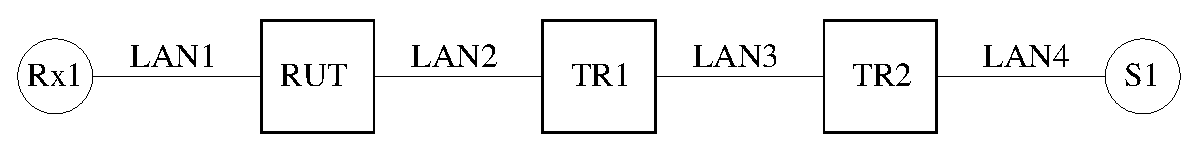
\includegraphics[scale=0.8]{figs/pim_test_3_3_register_messages_reception}
    \caption{Register messages reception test setup}
    \label{fig:pim_test_3_3_register_messages_reception}
  \end{center}
\end{figure}

\para{Procedure:}

\subpara{Part A: Receiving Register messages at the RP when there is a
receiver.}

\begin{enumerate}

  \item Configure the RUT such that it is the RP.

  \item Start the RUT, TR1, and TR2. If necessary, wait intil the RP-set in
  the RUT, TR1, and TR2 converges.

  \item Start Rx1.

  \item Observe the messages transmitted by the RUT on LAN2, and the messages
  received by Rx1.

  \item Start S1.

  \item Stop Rx1.

  \item Start Rx1.

\end{enumerate}

\subpara{Part B: Receiving Register messages at the RP when there is no
receiver.}

\begin{enumerate}

  \item Configure the RUT such that it is the RP.

  \item Start the RUT, TR1, and TR2. If necessary, wait intil the RP-set in
  the RUT, TR1, and TR2 converges.

  \item Observe the messages transmitted by the RUT on LAN2, and the messages
  received by Rx1.

  \item Start S1.

  \item Start Rx1.

  \item Stop Rx1.

  \item Start Rx1.

\end{enumerate}

\subpara{Part C: Receiving Register messages at the non-RP.}

\begin{enumerate}

  \item Manually configure TR2 only to appears that the RUT is the
  RP. However, configure the RUT itself, and TR1 such that for both of them
  appear that TR1 is the RP.

  \item Start Rx1.

  \item Start S1.

\end{enumerate}


\para{Observable Results:}

\subpara{Part A:}

\begin{itemize}

  \item After S1 is started, the data messages it transmits should be
  encapsulated in PIM Register messages by TR2, and sent to the RP (the
  RUT). The RUT should decapsulate them, and forward the inner multicast
  packets down the shared multicast tree to Rx1.

  \item After Rx1 is stopped, the RUT should send PIM Register-Stop message to
  TR2 for each PIM Register message it receives from the RUT (including
  the PIM Null-Register messages). After receiving the first PIM Register-Stop
  message, TR2 should stop sending PIM Register messages to the RP (the RUT)
  with the encapsulated data packets from S1.
  However, from time to time TR2 should be sending PIM Null-Register
  messages to the RP (the RUT) with time interval between two messages a random
  value chosen uniformly from the interval \\
  (0.5 * \verb=Register_Suppression_Time=,
  1.5 * \verb=Register_Suppression_Time=) \\
  - \verb=Register_Probe_Time= \\
  = ( (0.5 * {\PimsmRegisterSuppressionTime}, 1.5 *
  {\PimsmRegisterSuppressionTime}) - {\PimsmRegisterProbeTime} ). \\
  To each PIM Null-Register message, the RP (the RUT) should respond with a
  PIM Register-Stop message, therefore TR2 should continue not to
  encapsulate the data packets from S1.

  \item After Rx1 is started again, the RUT should send an SPT (S,G) Join
  message on LAN2 toward the source. As a result, the data packets from S1
  should be forwarded to the RP (the RUT) natively instead of encapsulating
  them in PIM Register messages.

\end{itemize}

\subpara{Part B:}

\begin{itemize}

  \item After S1 is started, the first one or few data messages it transmits
  should be encapsulated in PIM Register messages by TR2, and sent to the RP
  (the RUT). The RUT should respond to each PIM Register message with a PIM
  Register-Stop message for source S1 and group 224.0.1.20. After TR2 receives
  the first Register-Stop message, it should stop encapsulating the data
  packets and sending them to the RP (the RUT).

  \item From time to time TR2 should be sending PIM Null-Register
  messages to the RP (the RUT) with time interval between two messages a random
  value chosen uniformly from the interval \\
  (0.5 * \verb=Register_Suppression_Time=,
  1.5 * \verb=Register_Suppression_Time=) \\
  - \verb=Register_Probe_Time= \\
  = ( (0.5 * {\PimsmRegisterSuppressionTime}, 1.5 *
  {\PimsmRegisterSuppressionTime}) - {\PimsmRegisterProbeTime} ). \\
  To each PIM Null-Register message, the RP (the RUT) should respond with a
  PIM Register-Stop message, therefore TR2 should continue not to
  encapsulate the data packets from S1.

  \item After Rx1 is started, the RUT should send an SPT (S,G) Join message
  on LAN2 toward the source. As a result, the data packets from S1 should be
  forwarded to the RP (the RUT) natively instead of encapsulating them in PIM
  Register messages.

  \item After Rx1 is stopped, the RUT should send an SPT (S,G) Prune message
  on LAN2 toward the source. As a result, the data packets from S1 should not
  be forwarded by TR2 from LAN4 on LAN3.

  \item After Rx1 is started again, the RUT should send an SPT (S,G) Join
  message on LAN2 toward the source. As a result, the data packets from S1
  should be again be forwarded to the RP (the RUT) natively instead of
  encapsulating them in PIM Register messages.

\end{itemize}

\subpara{Part C:}

\begin{itemize}

  \item After S1 is started, the first one or few data messages it transmits
  should be encapsulated in PIM Register messages by TR2, and sent to the RUT,
  which TR2 thinks is the RP for group 224.0.1.20.
  However, because the RUT is not the RP, it should respond to each PIM
  Register message with a PIM Register-Stop message for source S1 and group
  224.0.1.20. After TR2 receives the first Register-Stop message, it should
  stop encapsulating the data packets and sending them to the RUT.

  \item From time to time TR2 should be sending PIM Null-Register
  messages to the RUT with time interval between two messages a random
  value chosen uniformly from the interval \\
  (0.5 * \verb=Register_Suppression_Time=,
  1.5 * \verb=Register_Suppression_Time=) \\
  - \verb=Register_Probe_Time= \\
  = ( (0.5 * {\PimsmRegisterSuppressionTime}, 1.5 *
  {\PimsmRegisterSuppressionTime}) - {\PimsmRegisterProbeTime} ). \\
  To each PIM Null-Register message, the RUT should respond with a
  PIM Register-Stop message, therefore TR2 should continue not to
  encapsulate the data packets from S1.

\end{itemize}

\para{Possible Problems:}
None.


%%%%%%%%%%%%%%%%%%%%%%%%%%%%%%%%%%%%%%%%%%%%%%%%%%%%%%%%%%%%%%%%%%%%%%%
\chapter{PIM Join/Prune Messages}

\para{Scope:}
Test sending and receiving of PIM Join/Prune messages.

\para{Overview:}
A PIM Join/Prune message consists of a list of groups and a list of
Joined and Pruned source for each group. It is used by the router
originating it to express interest (or lack of interest) in receiving
multicast traffic for specific groups and sources.

A Join/Prune message may contain four types of entries. An (*,G)
Join/Prune entry is sent toward the RP for group G, and is used to
express interest in receiving multicast packets from all sources for
that group. An (S,G) Join/Prune entry is sent toward the specified
source S, and is used to express interest in receiving multicast packets
from the specified source S and group G. An (S,G,rpt) Prune entry is
sent toward the RP for group G, and is used to stop receiving multicast
packets on the shared tree for the specified source S (note that there
is no (S,G,rpt) Join entry, because the (*,G) entry is used for that
purpose). An (*,*,RP) Join/Prune entry is sent toward the specified RP,
and is used to express interest in receiving multicast packets for all
multicast groups that use the specified RP as the root of their shared
trees.

The Join/Prune messages are sent either periodic or are triggered by
some events. Typically, all Join messages and the (S,G,rpt) Prune
messages are sent periodically.

%%%%%%%%%%%%%%%%%%%%%%%%%%%%%%%%%%%%%%%%%%%
\newpage
\section{Receiving (*,*,RP) Join/Prune Messages}

\para{Purpose:}
Verify that (*,*,RP) Join/Prune messages are received and processed
properly.

\para{References:}
\begin{itemize}
  \item draft-ietf-pim-sm-v2-new-05 -- Section 4.5.1
\end{itemize}

\para{Discussion:}
When a PIM-SM router receives a PIM (*,*,RP) Join/Prune message, the
per-interface (*,*,RP) state machine should be updated appropriately.
Typically, if an (*,*,RP) Join message is received, the interface it was
received on should be added to the set of outgoing interfaces to
forward packets destined for any group handled by the specified RP.
If that set has just became non-empty, an (*,*,RP) Join should be sent
toward the RP.
If an (*,*,RP) Prune message is received, typically it should remove
the interface it was received on from the set of outgoing interfaces
to forward packets destined to any group handled by the specified RP. If
that set has just became empty, an (*,*,RP) Prune message should be
sent toward the RP.

\para{Test Setup:}
Connect the RUT, TR1, TR2, TR3, S1, and S2 according to
Figure~\ref{fig:pim_test_4_1_receiving_rp_join_prune_messages}~\footnote{Note
that S1 is used only when TR3 and S2 are not used, hence it is not necessary
to have two senders at same time.}.
Enable PIM-SM on the RUT, TR1, TR2, and TR3.
Configure S1 and S2 as senders for group 224.0.1.20.

\begin{figure}[htbp]
  \begin{center}
    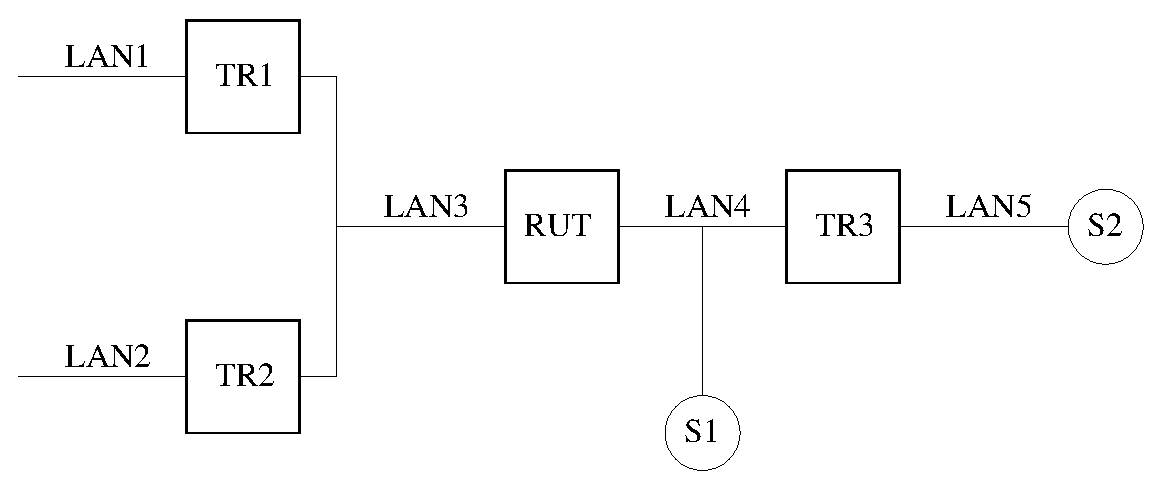
\includegraphics[scale=0.8]{figs/pim_test_4_1_receiving_rp_join_prune_messages}
    \caption{Receiving (*,*,RP) Join/Prune messages test setup}
    \label{fig:pim_test_4_1_receiving_rp_join_prune_messages}
  \end{center}
\end{figure}

\para{Procedure:}

\subpara{Part A: Receiving (*,*,RP) Join messages at the RP.}

\begin{enumerate}

  \item Configure the RUT as the RP. Start the RUT and TR1. If
  necessary, wait until the RP-set in the RUT and TR1 converges.

  \item Start observing the downstream (*,*,RP) per-interface state
  machine at the RUT.

  \item Compose an (*,*,RP) Join message at TR1 with the RP address set
  to the address of the RUT, and send it to the RUT.
  The \verb=J/P_HoldTime= of the message should be set to its default
  value ({\PimsmJPHoldTime}).

  \item Start S1, and observe the data packets transmitted by the RUT on
  LAN3.

  \item Wait until the downstream (*,*,RP) per-interface state in the RUT
  expires.

  \item Observe the data packets transmitted by the RUT on LAN3.

\end{enumerate}

\subpara{Part B: Receiving (*,*,RP) Prune messages at the RP.}

\begin{enumerate}

  \item Configure the RUT as the RP. Start the RUT and TR1. If
  necessary, wait until the RP-set in the RUT and TR1 converges.

  \item Start observing the downstream (*,*,RP) per-interface state
  machine at the RUT.

  \item Compose an (*,*,RP) Prune message at TR1 with the RP address set
  to the address of the RUT, and send it to the RUT.
  The \verb=J/P_HoldTime= of the message should be set to its default
  value ({\PimsmJPHoldTime}).

  \item Compose an (*,*,RP) Join message at TR1 with the RP address set
  to the address of the RUT, and send it to the RUT.
  The \verb=J/P_HoldTime= of the message should be set to its default
  value ({\PimsmJPHoldTime}).

  \item Start S1, and observe the data packets transmitted by the RUT on
  LAN3.

  \item Compose an (*,*,RP) Prune message at TR1 with the RP address set
  to the address of the RUT, and send it to the RUT.

  \item Observe the messages and data packets transmitted by the RUT on
  LAN3.

\end{enumerate}

\subpara{Part C: Receiving (*,*,RP) Join messages at non-RP router.}

\begin{enumerate}

  \item Configure TR3 as the RP. Start the RUT, TR1, and TR3. If
  necessary, wait until the RP-set in the RUT, TR1, and TR3
  converges.

  \item Start observing the downstream (*,*,RP) per-interface state
  machine at the RUT.

  \item Compose an (*,*,RP) Join message at TR1 with the RP address set
  to the address of TR3, and send it to the RUT.
  The \verb=J/P_HoldTime= of the message should be set to its default
  value ({\PimsmJPHoldTime}).

  \item Observe the messages transmitted by the RUT on LAN4.

  \item Start S2, and observe the data packets transmitted by the RUT on
  LAN3.

  \item Wait until the downstream (*,*,RP) per-interface state in the RUT
  expires.

  \item Observe the data packets transmitted by the RUT on LAN3.

\end{enumerate}

\subpara{Part D: Receiving (*,*,RP) Prune messages at non-RP router.}

\begin{enumerate}

  \item Configure TR3 as the RP. Start the RUT, TR1, and TR3. If
  necessary, wait until the RP-set in the RUT, TR1, and TR3
  converges.

  \item Start observing the downstream (*,*,RP) per-interface state
  machine at the RUT.

  \item Compose an (*,*,RP) Prune message at TR1 with the RP address set
  to the address of TR3, and send it to the RUT.
  The \verb=J/P_HoldTime= of the message should be set to its default
  value ({\PimsmJPHoldTime}).

  \item Compose an (*,*,RP) Join message at TR1 with the RP address set
  to the address of TR3, and send it to the RUT.
  The \verb=J/P_HoldTime= of the message should be set to its default
  value ({\PimsmJPHoldTime}).

  \item Observe the messages transmitted by the RUT on LAN4.

  \item Start S2, and observe the data packets transmitted by the RUT on
  LAN3.

  \item Compose an (*,*,RP) Prune message at TR1 with the RP address set
  to the address of TR3, and send it to the RUT.

  \item Observe the messages transmitted by the RUT on LAN3 and LAN4,
  and the data packets transmitted by the RUT on LAN3.

\end{enumerate}

\subpara{Part E: Receiving (*,*,RP) Prune messages on a LAN.}

This part is same as Part D, except that in Step 1 we start TR2 as well.

\subpara{Part F: Receiving (*,*,RP) Join and Prune messages on a LAN.}

This part is same as Part E, except that in Step 2 we compose and send
same (*,*,RP) Join message from TR2 as well.

\para{Observable Results:}

\subpara{Part A:}

\begin{itemize}

  \item After the (*,*,RP) Join message is received by the RUT, it
  should create the appropriate (*,*,RP) multicast routing entry for
  that RP, and the interface toward LAN3 should be in Join state and
  added to the set of outgoing interface for that entry:

\begin{verbatim}
Xorp> show pim join 
Group           Source          RP              Flags
224.0.0.0       10.3.0.1        10.3.0.1        RP   
    Upstream interface (S):    UNKNOWN
    Upstream interface (RP):   register_vif
    Upstream MRIB next hop (RP): UNKNOWN
    Upstream MRIB next hop (S):  UNKNOWN
    Upstream RPF'(*,G):        UNKNOWN
    Upstream RPF'(S,G):        UNKNOWN
    Upstream RPF'(S,G,rpt):    UNKNOWN
    Upstream state:            Joined 
    Register state:            
    Join timer:                52
    Joins RP:                  ......O.......
    Join state:                ......O.......
    Prune state:               ..............
    Prune pending state:       ..............
    Could assert WC:           ......O.......
    I am DR:                   .....OO.......
    Immediate olist RP:        ......O.......
    Inherited olist SG:        ..............
    Inherited olist SG_RPT:    ..............
\end{verbatim}

  \item After S1 is started, the multicast data packets should be
  forwarded by the RUT on LAN3.

  \item After \verb=J/P_HoldTime= ({\PimsmJPHoldTime}),
  the (*,*,RP) state machine for the interface that connects the RUT to
  LAN3 should timeout and transition to NoInfo state
  (\ie the (*,*,RP) entry in the RUT should expire).
  As a result of that transition, no multicast packets should be
  forwarded by the RUT on LAN3.

\end{itemize}

\subpara{Part B:}

\begin{itemize}

  \item After the (*,*,RP) Prune message is received by the RUT,
  the (*,*,RP) state machine for the interface that connects the RUT to
  LAN3 should continue to stay in the NoInfo state (\ie no (*,*,RP) multicast
  routing entry should be created).
  
  \item After that, the results until after S1 is started should be same as in
  Part A.

  \item After the (*,*,RP) Prune message is received by the RUT,
  the (*,*,RP) state machine for the interface that connects the RUT to
  LAN3 should transition to NoInfo state
  (\ie the (*,*,RP) entry in the RUT should expire).
  As a result of that transition no multicast packets should be
  forwarded by the RUT on LAN3.

\end{itemize}

\subpara{Part C:}

\begin{itemize}

  \item After the (*,*,RP) Join message is received by the RUT, it
  should create the appropriate (*,*,RP) multicast routing entry for
  that RP, and the interface toward LAN3 should be in Join state and
  added to the set of outgoing interface for that entry:

\begin{verbatim}
Xorp> show pim join 
Group           Source          RP              Flags
224.0.0.0       10.9.0.1        10.9.0.1        RP   
    Upstream interface (S):    UNKNOWN
    Upstream interface (RP):   dc1
    Upstream MRIB next hop (RP): 10.3.0.2
    Upstream MRIB next hop (S):  UNKNOWN
    Upstream RPF'(*,G):        UNKNOWN
    Upstream RPF'(S,G):        UNKNOWN
    Upstream RPF'(S,G,rpt):    UNKNOWN
    Upstream state:            Joined 
    Register state:            
    Join timer:                47
    Joins RP:                  ......O.......
    Join state:                ......O.......
    Prune state:               ..............
    Prune pending state:       ..............
    Could assert WC:           ......O.......
    I am DR:                   ......O.......
    Immediate olist RP:        ......O.......
    Inherited olist SG:        ..............
    Inherited olist SG_RPT:    ..............
\end{verbatim}

  Further, the RUT itself should originate an (*,*,RP) Join message
  toward the RP (TR3).

  \item After S2 is started, the multicast data packets forwarded by TR3
  on LAN4 should be forwarded by the RUT on LAN3.

  \item After \verb=J/P_HoldTime= ({\PimsmJPHoldTime}),
  the (*,*,RP) state machine for the interface that connects the RUT to
  LAN3 should timeout and transition to NoInfo state
  (\ie the (*,*,RP) entry in the RUT should expire).
  As a result of that transition, the RUT should send (*,*,RP) Prune
  message toward the RP (TR3), and no multicast packets should be
  forwarded by the RUT on LAN3.

\end{itemize}

\subpara{Part D:}

\begin{itemize}

  \item After the (*,*,RP) Prune message is received by the RUT,
  the (*,*,RP) state machine for the interface that connects the RUT to
  LAN3 should continue to stay in the NoInfo state (\ie no (*,*,RP) multicast
  routing entry should be created).

  \item After that, the results until after S2 is started should be same as in
  Part C.

  \item After the (*,*,RP) Prune message from TR1 is received by the RUT,
  the (*,*,RP) state machine for the interface that connects the RUT to
  LAN3 should transition to NoInfo state
  (\ie the (*,*,RP) entry in the RUT should expire).
  As a result of that transition, the RUT should send (*,*,RP) Prune
  message toward the RP (TR3), and no multicast packets should be
  forwarded by the RUT on LAN3. Note that because the RUT has only one
  PIM neighbor on LAN3, it does not need to send (*,*,RP) PruneEcho on
  LAN3.

\end{itemize}

\subpara{Part E:}

\begin{itemize}

  \item The results until after S2 is started should be same as in
  Part C and D.

  \item After the (*,*,RP) Prune message from TR1 is received by the RUT,
  the (*,*,RP) state machine for the interface that connects the RUT to
  LAN3 should transition to Prune-Pending state (the reason that it does
  not transit to NoInfo instead is because the RUT has more than one PIM
  neighbors on that interface).
  After \verb=J/P_Override_Interval(I)= (\PimsmJPOverrideIntervalI),
  the Prune-Pending Timer on that interface should expire, and the
  (*,*,RP) state machine for the interface should send (*,*,RP) PruneEcho
  on LAN3 and transit to NoInfo
  state (\ie the (*,*,RP) entry in the RUT should expire).
  As a result of that transition, the RUT should send (*,*,RP) Prune
  message toward the RP (TR3), and no multicast packets should be
  forwarded by the RUT on LAN3.

\end{itemize}

\subpara{Part F:}

\begin{itemize}

  \item The results until after S2 is started should be same as in
  Part C, D, and E.

  \item After the (*,*,RP) Prune message from TR1 is received by the RUT,
  the (*,*,RP) state machine for the interface that connects the RUT to
  LAN3 should transition to Prune-Pending state (the reason that it does
  not transit to NoInfo instead is because the RUT has more than one PIM
  neighbors on that interface).
  Assuming that TR2 has (*,*,RP) multicast routing entry in Joined state
  for the RP it had originated (*,*,RP) Join message earlier, then after
  very short random interval \verb=t_override= ({\PimsmTOverride}) TR2
  should send another (*,*,RP) Join message to the RUT.
  After the RUT receives that (*,*,RP) Join message from TR2,
  the (*,*,RP) state machine for the interface that connects the RUT to
  LAN3 should transition back to Join state.
  As a result of that transition, the RUT should not send (*,*,RP) Prune
  message toward the RP (TR3), and the multicast packets should continue
  to be forwarded by the RUT on LAN3.

\end{itemize}

\para{Possible Problems:}
None.

%%%%%%%%%%%%%%%%%%%%%%%%%%%%%%%%%%%%%%%%%%%
\newpage
\section{Receiving (*,G) Join/Prune Messages}

\para{Purpose:}
Verify that (*,G) Join/Prune messages are received and processed
properly.

\para{References:}
\begin{itemize}
  \item draft-ietf-pim-sm-v2-new-05 -- Section 4.5.2
\end{itemize}

\para{Discussion:}
When a PIM-SM router receives a PIM (*,G) Join/Prune message, the
per-interface (*,G) state machine should be updated appropriately.
Typically, if an (*,G) Join message is received, the interface it was
received on should be added to the set of outgoing interfaces to
forward packets destined for the specified multicast group address.
If that set has just became non-empty, an (*,G) Join should be sent
toward the RP for that group.
If an (*,G) Prune message is received, typically it should remove
the interface it was received on from the set of outgoing interfaces
for that group. If
that set has just became empty, an (*,G) Prune message should be
sent toward the RP for that group.

\para{Test Setup:}
Connect the RUT, TR1, TR2, TR3, S1, and S2 according to
Figure~\ref{fig:pim_test_4_2_receiving_wc_join_prune_messages}~\footnote{Note
that S1 is used only when TR3 and S2 are not used, hence it is not necessary
to have two senders at same time.}.
Enable PIM-SM on the RUT, TR1, TR2, and TR3.
Configure S1 and S2 as senders for group 224.0.1.20.

\begin{figure}[htbp]
  \begin{center}
    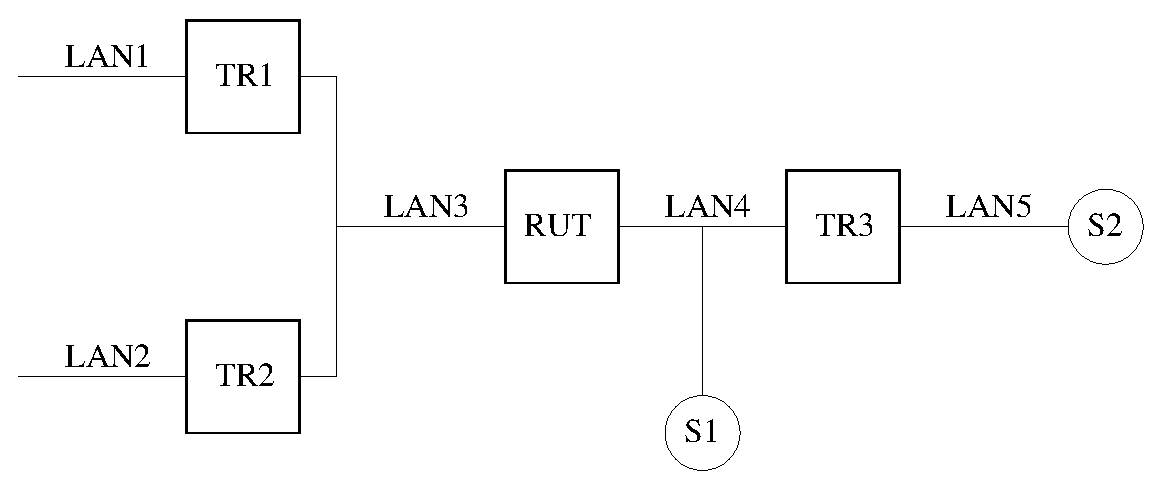
\includegraphics[scale=0.8]{figs/pim_test_4_2_receiving_wc_join_prune_messages}
    \caption{Receiving (*,G) Join/Prune messages test setup}
    \label{fig:pim_test_4_2_receiving_wc_join_prune_messages}
  \end{center}
\end{figure}

\para{Procedure:}

\subpara{Part A: Receiving (*,G) Join messages at the RP.}

\begin{enumerate}

  \item Configure the RUT as the RP. Start the RUT and TR1. If
  necessary, wait until the RP-set in the RUT and TR1 converges.

  \item Start observing the downstream (*,G) per-interface state
  machine at the RUT.

  \item Compose an (*,G) Join message at TR1 with the RP address set
  to the address of the RUT, and send it to the RUT.
  The \verb=J/P_HoldTime= of the message should be set to its default
  value ({\PimsmJPHoldTime}).

  \item Start S1, and observe the data packets transmitted by the RUT on
  LAN3.

  \item Wait until the downstream (*,G) per-interface state in the RUT
  expires.

  \item Observe the data packets transmitted by the RUT on LAN3.

\end{enumerate}

\subpara{Part B: Receiving (*,G) Prune messages at the RP.}

\begin{enumerate}

  \item Configure the RUT as the RP. Start the RUT and TR1. If
  necessary, wait until the RP-set in the RUT and TR1 converges.

  \item Start observing the downstream (*,G) per-interface state
  machine at the RUT.

  \item Compose an (*,G) Prune message at TR1 with the RP address set
  to the address of the RUT, and send it to the RUT.
  The \verb=J/P_HoldTime= of the message should be set to its default
  value ({\PimsmJPHoldTime}).

  \item Compose an (*,G) Join message at TR1 with the RP address set
  to the address of the RUT, and send it to the RUT.
  The \verb=J/P_HoldTime= of the message should be set to its default
  value ({\PimsmJPHoldTime}).

  \item Start S1, and observe the data packets transmitted by the RUT on
  LAN3.

  \item Compose an (*,G) Prune message at TR1 with the RP address set
  to the address of the RUT, and send it to the RUT.

  \item Observe the messages and data packets transmitted by the RUT on
  LAN3.

\end{enumerate}

\subpara{Part C: Receiving (*,G) Join messages at non-RP router.}

\begin{enumerate}

  \item Configure TR3 as the RP. Start the RUT, TR1, and TR3. If
  necessary, wait until the RP-set in the RUT, TR1, and TR3
  converges.

  \item Start observing the downstream (*,G) per-interface state
  machine at the RUT.

  \item Compose an (*,G) Join message at TR1 with the RP address set
  to the address of TR3, and send it to the RUT.
  The \verb=J/P_HoldTime= of the message should be set to its default
  value ({\PimsmJPHoldTime}).

  \item Observe the messages transmitted by the RUT on LAN4.

  \item Start S2, and observe the data packets transmitted by the RUT on
  LAN3.

  \item Wait until the downstream (*,G) per-interface state in the RUT
  expires.

  \item Observe the data packets transmitted by the RUT on LAN3.

\end{enumerate}

\subpara{Part D: Receiving (*,G) Prune messages at non-RP router.}

\begin{enumerate}

  \item Configure TR3 as the RP. Start the RUT, TR1, and TR3. If
  necessary, wait until the RP-set in the RUT, TR1, and TR3
  converges.

  \item Start observing the downstream (*,G) per-interface state
  machine at the RUT.

  \item Compose an (*,G) Prune message at TR1 with the RP address set
  to the address of TR3, and send it to the RUT.
  The \verb=J/P_HoldTime= of the message should be set to its default
  value ({\PimsmJPHoldTime}).

  \item Compose an (*,G) Join message at TR1 with the RP address set
  to the address of TR3, and send it to the RUT.
  The \verb=J/P_HoldTime= of the message should be set to its default
  value ({\PimsmJPHoldTime}).

  \item Observe the messages transmitted by the RUT on LAN4.

  \item Start S2, and observe the data packets transmitted by the RUT on
  LAN3.

  \item Compose an (*,G) Prune message at TR1 with the RP address set
  to the address of TR3, and send it to the RUT.

  \item Observe the messages transmitted by the RUT on LAN3 and LAN4,
  and the data packets transmitted by the RUT on LAN3.

\end{enumerate}

\subpara{Part E: Receiving (*,G) Prune messages on a LAN.}

This part is same as Part D, except that in Step 1 we start TR2 as well.

\subpara{Part F: Receiving (*,G) Join and Prune messages on a LAN.}

This part is same as Part E, except that in Step 2 we compose and send
same (*,G) Join message from TR2 as well.

\subpara{Part G: Receiving (*,G) Join messages with mismatch RP address at
non-RP router}

\begin{enumerate}

  \item Configure TR3 as the RP. Start the RUT, TR1, and TR3. If
  necessary, wait until the RP-set in the RUT, TR1, and TR3
  converges.

  \item Start observing the downstream (*,G) per-interface state
  machine at the RUT.

  \item Compose an (*,G) Join message at TR1 with the RP address set
  to an address that is different from the address of TR3, but such that
  TR3 is the next-hop router toward it (\eg the address of S), and send it to
  the RUT.
  The \verb=J/P_HoldTime= of the message should be set to its default
  value ({\PimsmJPHoldTime}).

  \item Observe the messages transmitted by the RUT on LAN4.

\end{enumerate}

\para{Observable Results:}

\subpara{Part A:}

\begin{itemize}

  \item After the (*,G) Join message is received by the RUT, it
  should create the appropriate (*,G) multicast routing entry for
  that group, and the interface toward LAN3 should be in Join state and
  added to the set of outgoing interface for that entry:

\begin{verbatim}
Xorp> show pim join 
Group           Source          RP              Flags
224.0.1.20      0.0.0.0         10.3.0.1        WC   
    Upstream interface (RP):   register_vif
    Upstream MRIB next hop (RP): UNKNOWN
    Upstream RPF'(*,G):        UNKNOWN
    Upstream state:            Joined 
    Register state:            
    Join timer:                42
    Local receiver include WC: ..............
    Joins RP:                  ..............
    Joins WC:                  ......O.......
    Join state:                ......O.......
    Prune state:               ..............
    Prune pending state:       ..............
    I am assert winner state:  ..............
    I am assert loser state:   ..............
    Assert winner WC:          ..............
    Assert lost WC:            ..............
    Assert tracking WC:        ......O......O
    Could assert WC:           ......O.......
    I am DR:                   .....OO.......
    Immediate olist RP:        ..............
    Immediate olist WC:        ......O.......
    Inherited olist SG:        ..............
    Inherited olist SG_RPT:    ..............
    PIM include WC:            ..............
\end{verbatim}

  \item After S1 is started, the multicast data packets should be
  forwarded by the RUT on LAN3.

  \item After \verb=J/P_HoldTime= ({\PimsmJPHoldTime}),
  the (*,G) state machine for the interface that connects the RUT to
  LAN3 should timeout and transition to NoInfo state
  (\ie the (*,G) entry in the RUT should expire).
  As a result of that transition, no multicast packets should be
  forwarded by the RUT on LAN3.

\end{itemize}

\subpara{Part B:}

\begin{itemize}

  \item After the (*,G) Prune message is received by the RUT,
  the (*,G) state machine for the interface that connects the RUT to
  LAN3 should continue to stay in the NoInfo state (\ie no (*,G) multicast
  routing entry should be created).

  \item After that, the results until after S1 is started should be same as in
  Part A.

  \item After the (*,G) Prune message is received by the RUT,
  the (*,G) state machine for the interface that connects the RUT to
  LAN3 should transition to NoInfo state
  (\ie the (*,G) entry in the RUT should expire).
  As a result of that transition no multicast packets should be
  forwarded by the RUT on LAN3.

\end{itemize}

\subpara{Part C:}

\begin{itemize}

  \item After the (*,G) Join message is received by the RUT, it
  should create the appropriate (*,G) multicast routing entry for
  that group, and the interface toward LAN3 should be in Join state and
  added to the set of outgoing interface for that entry:

\begin{verbatim}
Xorp> show pim join 
Group           Source          RP              Flags
224.0.1.20      0.0.0.0         10.4.0.1        WC   
    Upstream interface (RP):   dc1
    Upstream MRIB next hop (RP): 10.3.0.2
    Upstream RPF'(*,G):        10.3.0.2
    Upstream state:            Joined 
    Register state:            
    Join timer:                50
    Local receiver include WC: ..............
    Joins RP:                  ..............
    Joins WC:                  ......O.......
    Join state:                ......O.......
    Prune state:               ..............
    Prune pending state:       ..............
    I am assert winner state:  ..............
    I am assert loser state:   ..............
    Assert winner WC:          ..............
    Assert lost WC:            ..............
    Assert tracking WC:        .....OO.......
    Could assert WC:           ......O.......
    I am DR:                   ......O.......
    Immediate olist RP:        ..............
    Immediate olist WC:        ......O.......
    Inherited olist SG:        ..............
    Inherited olist SG_RPT:    ..............
    PIM include WC:            ..............
\end{verbatim}

  Further, the RUT itself should originate an (*,G) Join message
  toward the RP (TR3).

  \item After S2 is started, the multicast data packets forwarded by TR3
  on LAN4 should be forwarded by the RUT on LAN3.

  \item After \verb=J/P_HoldTime= ({\PimsmJPHoldTime}),
  the (*,G) state machine for the interface that connects the RUT to
  LAN3 should timeout and transition to NoInfo state
  (\ie the (*,G) entry in the RUT should expire).
  As a result of that transition, the RUT should send (*,G) Prune
  message toward the RP (TR3), and no multicast packets should be
  forwarded by the RUT on LAN3.

\end{itemize}

\subpara{Part D:}

\begin{itemize}

  \item After the (*,G) Prune message is received by the RUT,
  the (*,G) state machine for the interface that connects the RUT to
  LAN3 should continue to stay in the NoInfo state (\ie no (*,G) multicast
  routing entry should be created).

  \item After that, the results until after S2 is started should be same as in
  Part C.

  \item After the (*,G) Prune message from TR1 is received by the RUT,
  the (*,G) state machine for the interface that connects the RUT to
  LAN3 should transition to NoInfo state
  (\ie the (*,G) entry in the RUT should expire).
  As a result of that transition, the RUT should send (*,G) Prune
  message toward the RP (TR3), and no multicast packets should be
  forwarded by the RUT on LAN3. Note that because the RUT has only one
  PIM neighbor on LAN3, it does not need to send (*,G) PruneEcho on
  LAN3.

\end{itemize}

\subpara{Part E:}

\begin{itemize}

  \item The results until after S2 is started should be same as in
  Part C and D.

  \item After the (*,G) Prune message from TR1 is received by the RUT,
  the (*,G) state machine for the interface that connects the RUT to
  LAN3 should transition to Prune-Pending state (the reason that it does
  not transit to NoInfo instead is because the RUT has more than one PIM
  neighbors on that interface).
  After \verb=J/P_Override_Interval(I)= (\PimsmJPOverrideIntervalI),
  the Prune-Pending Timer on that interface should expire, and the
  (*,G) state machine for the interface should send (*,G) PruneEcho
  on LAN3 and transit to NoInfo
  state (\ie the (*,G) entry in the RUT should expire).
  As a result of that transition, the RUT should send (*,G) Prune
  message toward the RP (TR3), and no multicast packets should be
  forwarded by the RUT on LAN3.

\end{itemize}

\subpara{Part F:}

\begin{itemize}

  \item The results until after S2 is started should be same as in
  Part C, D, and E.

  \item After the (*,G) Prune message from TR1 is received by the RUT,
  the (*,G) state machine for the interface that connects the RUT to
  LAN3 should transition to Prune-Pending state (the reason that it does
  not transit to NoInfo instead is because the RUT has more than one PIM
  neighbors on that interface).
  Assuming that TR2 has (*,G) multicast routing entry in Joined state
  for the RP it had originated (*,G) Join message earlier, then after
  very short random interval \verb=t_override= ({\PimsmTOverride}) TR2
  should send another (*,G) Join message to the RUT.
  After the RUT receives that (*,G) Join message from TR2,
  the (*,G) state machine for the interface that connects the RUT to
  LAN3 should transition back to Join state.
  As a result of that transition, the RUT should not send (*,G) Prune
  message toward the RP (TR3), and the multicast packets should continue
  to be forwarded by the RUT on LAN3.

\end{itemize}

\subpara{Part G:}

\begin{itemize}
  \item After the RUT receives the (*,G) Join message with the mismatch RP
  address inside, it should silently ignore it without any further action.
\end{itemize}

\para{Possible Problems:}
None.


%%%%%%%%%%%%%%%%%%%%%%%%%%%%%%%%%%%%%%%%%%%
\newpage
\section{Receiving (S,G) Join/Prune Messages}

\para{Purpose:}
Verify that (S,G) Join/Prune messages are received and processed
properly.

\para{References:}
\begin{itemize}
  \item draft-ietf-pim-sm-v2-new-05 -- Section 4.5.3
\end{itemize}

\para{Discussion:}
When a PIM-SM router receives a PIM (S,G) Join/Prune message, the
per-interface (S,G) state machine should be updated appropriately.
Typically, if an (S,G) Join message is received, the interface it was
received on should be added to the set of outgoing interfaces to
forward packets destined for the specified source address and multicast group.
If that set has just became non-empty, an (S,G) Join should be sent
toward the specified source.
If an (S,G) Prune message is received, typically it should remove
the interface it was received on from the set of outgoing interfaces
for that source and group. If
that set has just became empty, an (S,G) Prune message should be
sent toward the source.

\para{Test Setup:}
Connect the RUT, TR1, TR2, TR3, S1, and S2 according to
Figure~\ref{fig:pim_test_4_3_receiving_sg_join_prune_messages}~\footnote{Note
that S1 is used only when TR3 and S2 are not used, hence it is not necessary
to have two senders at same time.}.
Enable PIM-SM on the RUT, TR1, TR2, and TR3.
Configure S1 and S2 as senders for group 224.0.1.20.

\begin{figure}[htbp]
  \begin{center}
    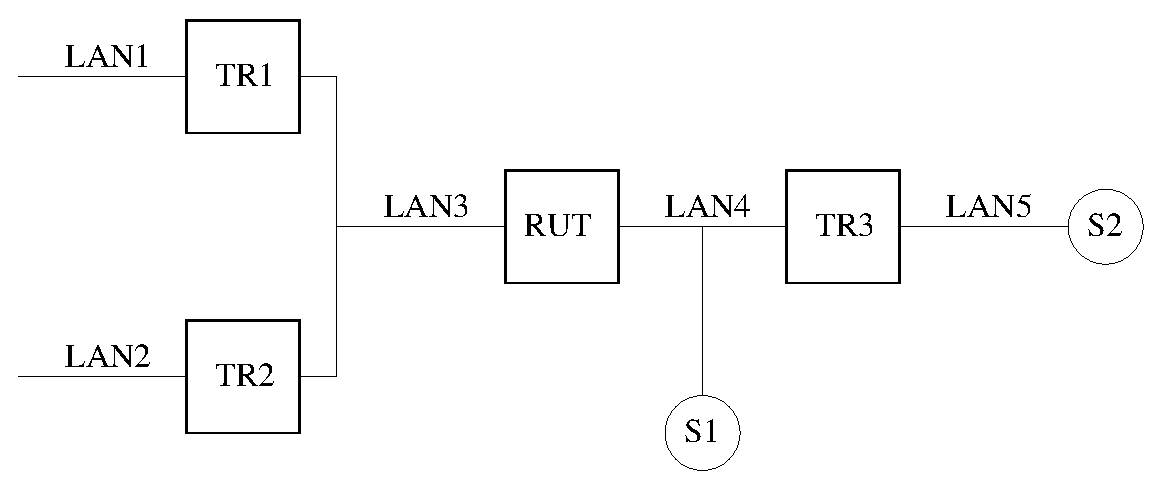
\includegraphics[scale=0.8]{figs/pim_test_4_3_receiving_sg_join_prune_messages}
    \caption{Receiving (S,G) Join/Prune messages test setup}
    \label{fig:pim_test_4_3_receiving_sg_join_prune_messages}
  \end{center}
\end{figure}

\para{Procedure:}

\subpara{Part A: Receiving (S,G) Join messages at the first-hop router.}

\begin{enumerate}

  \item Configure the RUT as the RP. Start the RUT and TR1. If
  necessary, wait until the RP-set in the RUT and TR1 converges.

  \item Start observing the downstream (S,G) per-interface state
  machine at the RUT.

  \item Compose an (S,G) Join message at TR1 with the source address set
  to the address of S1, and send it to the RUT.
  The \verb=J/P_HoldTime= of the message should be set to its default
  value ({\PimsmJPHoldTime}).

  \item Start S1, and observe the data packets transmitted by the RUT on
  LAN3.

  \item Wait until the downstream (S,G) per-interface state in the RUT
  expires.

  \item Observe the data packets transmitted by the RUT on LAN3.

  \item Stop S1.

\end{enumerate}

\subpara{Part B: Receiving (S,G) Prune messages at the first-hop router.}

\begin{enumerate}

  \item Configure the RUT as the RP. Start the RUT and TR1. If
  necessary, wait until the RP-set in the RUT and TR1 converges.

  \item Start observing the downstream (S,G) per-interface state
  machine at the RUT.

  \item Compose an (S,G) Prune message at TR1 with the source address set
  to the address of S1, and send it to the RUT.
  The \verb=J/P_HoldTime= of the message should be set to its default
  value ({\PimsmJPHoldTime}).

  \item Compose an (S,G) Join message at TR1 with the source address set
  to the address of S1, and send it to the RUT.
  The \verb=J/P_HoldTime= of the message should be set to its default
  value ({\PimsmJPHoldTime}).

  \item Start S1, and observe the data packets transmitted by the RUT on
  LAN3.

  \item Compose an (S,G) Prune message at TR1 with the source address set
  to the address of S1, and send it to the RUT.

  \item Observe the messages and data packets transmitted by the RUT on
  LAN3.

  \item Stop S1.

\end{enumerate}

\subpara{Part C: Receiving (S,G) Join messages at non-first-hop router.}

\begin{enumerate}

  \item Configure TR3 as the RP. Start the RUT, TR1, and TR3. If
  necessary, wait until the RP-set in the RUT, TR1, and TR3
  converges.

  \item Start observing the downstream (S,G) per-interface state
  machine at the RUT.

  \item Compose an (S,G) Join message at TR1 with the source address set
  to the address of S2, and send it to the RUT.
  The \verb=J/P_HoldTime= of the message should be set to its default
  value ({\PimsmJPHoldTime}).

  \item Observe the messages transmitted by the RUT on LAN4.

  \item Start S2, and observe the data packets transmitted by the RUT on
  LAN3.

  \item Wait until the downstream (S,G) per-interface state in the RUT
  expires.

  \item Observe the data packets transmitted by the RUT on LAN3.

  \item Stop S2.

\end{enumerate}

\subpara{Part D: Receiving (S,G) Prune messages at non-first-hop router.}

\begin{enumerate}

  \item Configure TR3 as the RP. Start the RUT, TR1, and TR3. If
  necessary, wait until the RP-set in the RUT, TR1, and TR3
  converges.

  \item Start observing the downstream (S,G) per-interface state
  machine at the RUT.

  \item Compose an (S,G) Prune message at TR1 with the source address set
  to the address of S2, and send it to the RUT.
  The \verb=J/P_HoldTime= of the message should be set to its default
  value ({\PimsmJPHoldTime}).

  \item Compose an (S,G) Join message at TR1 with the source address set
  to the address of S2, and send it to the RUT.
  The \verb=J/P_HoldTime= of the message should be set to its default
  value ({\PimsmJPHoldTime}).

  \item Observe the messages transmitted by the RUT on LAN4.

  \item Start S2, and observe the data packets transmitted by the RUT on
  LAN3.

  \item Compose an (S,G) Prune message at TR1 with the source address set
  to the address of S2, and send it to the RUT.

  \item Observe the messages transmitted by the RUT on LAN3 and LAN4,
  and the data packets transmitted by the RUT on LAN3.

  \item Stop S2.

\end{enumerate}

\subpara{Part E: Receiving (S,G) Prune messages on a LAN.}

This part is same as Part D, except that in Step 1 we start TR2 as well.

\subpara{Part F: Receiving (S,G) Join and Prune messages on a LAN.}

This part is same as Part E, except that in Step 2 we compose and send
same (S,G) Join message from TR2 as well.

\para{Observable Results:}

\subpara{Part A:}

\begin{itemize}

  \item After the (S,G) Join message is received by the RUT, it
  should create the appropriate (S,G) multicast routing entry for
  that source and group, and the interface toward LAN3 should be in Join state
  and added to the set of outgoing interface for that entry:

\begin{verbatim}
Xorp> show pim join 
Group           Source          RP              Flags
224.0.1.20      10.3.0.2        10.3.0.1        SG DirectlyConnectedS 
    Upstream interface (S):    dc1
    Upstream interface (RP):   register_vif
    Upstream MRIB next hop (RP): UNKNOWN
    Upstream MRIB next hop (S):  UNKNOWN
    Upstream RPF'(S,G):        UNKNOWN
    Upstream state:            Joined 
    Register state:            RegisterNoinfo RegisterNotCouldRegister 
    Join timer:                51
    Local receiver include WC: ..............
    Local receiver include SG: ..............
    Local receiver exclude SG: ..............
    Joins RP:                  ..............
    Joins WC:                  ..............
    Joins SG:                  ......O.......
    Join state:                ......O.......
    Prune state:               ..............
    Prune pending state:       ..............
    I am assert winner state:  ..............
    I am assert loser state:   ..............
    Assert winner WC:          ..............
    Assert winner SG:          ..............
    Assert lost WC:            ..............
    Assert lost SG:            ..............
    Assert lost SG_RPT:        ..............
    Assert tracking SG:        .....OO.......
    Could assert WC:           ..............
    Could assert SG:           ..............
    I am DR:                   .....OO.......
    Immediate olist RP:        ..............
    Immediate olist WC:        ..............
    Immediate olist SG:        ......O.......
    Inherited olist SG:        ......O.......
    Inherited olist SG_RPT:    ..............
    PIM include WC:            ..............
    PIM include SG:            ..............
    PIM exclude SG:            ..............
\end{verbatim}

  \item After S1 is started, the multicast data packets should be
  forwarded by the RUT on LAN3. In addition, the SPT flag for the
  entry should be set:

\begin{verbatim}
Xorp> show pim join 
Group           Source          RP              Flags
224.0.1.20      10.3.0.2        10.3.0.1        SG SPT DirectlyConnectedS 
    Upstream interface (S):    dc1
    Upstream interface (RP):   register_vif
    Upstream MRIB next hop (RP): UNKNOWN
    Upstream MRIB next hop (S):  UNKNOWN
    Upstream RPF'(S,G):        UNKNOWN
    Upstream state:            Joined 
    Register state:            RegisterNoinfo RegisterNotCouldRegister 
    Join timer:                19
    Local receiver include WC: ..............
    Local receiver include SG: ..............
    Local receiver exclude SG: ..............
    Joins RP:                  ..............
    Joins WC:                  ..............
    Joins SG:                  ......O.......
    Join state:                ......O.......
    Prune state:               ..............
    Prune pending state:       ..............
    I am assert winner state:  ..............
    I am assert loser state:   ..............
    Assert winner WC:          ..............
    Assert winner SG:          ..............
    Assert lost WC:            ..............
    Assert lost SG:            ..............
    Assert lost SG_RPT:        ..............
    Assert tracking SG:        .....OO.......
    Could assert WC:           ..............
    Could assert SG:           ......O.......
    I am DR:                   .....OO.......
    Immediate olist RP:        ..............
    Immediate olist WC:        ..............
    Immediate olist SG:        ......O.......
    Inherited olist SG:        ......O.......
    Inherited olist SG_RPT:    ..............
    PIM include WC:            ..............
    PIM include SG:            ..............
    PIM exclude SG:            ..............
\end{verbatim}

  \item After \verb=J/P_HoldTime= ({\PimsmJPHoldTime}),
  the (S,G) state machine for the interface that connects the RUT to
  LAN3 should timeout and transition to NoInfo state.
  As a result of that transition, no multicast packets should be
  forwarded by the RUT on LAN3.
  However, the (S,G) entry itself should not be removed yet, because the
  directly-connected sender is still active:

\begin{verbatim}
Xorp> show pim join 
Group           Source          RP              Flags
224.0.1.20      10.3.0.2        10.3.0.1        SG DirectlyConnectedS 
    Upstream interface (S):    dc1
    Upstream interface (RP):   register_vif
    Upstream MRIB next hop (RP): UNKNOWN
    Upstream MRIB next hop (S):  UNKNOWN
    Upstream RPF'(S,G):        UNKNOWN
    Upstream state:            NotJoined 
    Register state:            RegisterNoinfo RegisterNotCouldRegister 
    Join timer:                -1
    Local receiver include WC: ..............
    Local receiver include SG: ..............
    Local receiver exclude SG: ..............
    Joins RP:                  ..............
    Joins WC:                  ..............
    Joins SG:                  ..............
    Join state:                ..............
    Prune state:               ..............
    Prune pending state:       ..............
    I am assert winner state:  ..............
    I am assert loser state:   ..............
    Assert winner WC:          ..............
    Assert winner SG:          ..............
    Assert lost WC:            ..............
    Assert lost SG:            ..............
    Assert lost SG_RPT:        ..............
    Assert tracking SG:        ..............
    Could assert WC:           ..............
    Could assert SG:           ..............
    I am DR:                   .....OO.......
    Immediate olist RP:        ..............
    Immediate olist WC:        ..............
    Immediate olist SG:        ..............
    Inherited olist SG:        ..............
    Inherited olist SG_RPT:    ..............
    PIM include WC:            ..............
    PIM include SG:            ..............
    PIM exclude WC:            ..............
\end{verbatim}

 \item After the sender is stopped, and after it has been inactive
  for \verb=Keepalive_Period= ({\PimsmKeepalivePeriod}), the (S,G) entry
  should expire.

\end{itemize}

\subpara{Part B:}

\begin{itemize}

  \item After the (S,G) Prune message is received by the RUT,
  the (S,G) state machine for the interface that connects the RUT to
  LAN3 should continue to stay in the NoInfo state (\ie no (S,G) multicast
  routing entry should be created).

  \item After that, the results until after S1 is started should be same as in
  Part A.

  \item After the (S,G) Prune message is received by the RUT,
  the (S,G) state machine for the interface that connects the RUT to
  LAN3 should transition to NoInfo state.
  As a result of that transition no multicast packets should be
  forwarded by the RUT on LAN3.
  However, the (S,G) entry itself should not be removed yet, because the
  directly-connected sender is still active (see Part A).

 \item After the sender is stopped, and after it has been inactive
  for \verb=Keepalive_Period= ({\PimsmKeepalivePeriod}), the (S,G) entry
  should expire.

\end{itemize}

\subpara{Part C:}

\begin{itemize}

  \item After the (S,G) Join message is received by the RUT, it
  should create the appropriate (S,G) multicast routing entry for
  that source and group, and the interface toward LAN3 should be in Join state
  and added to the set of outgoing interface for that entry:

\begin{verbatim}
Xorp> show pim join 
Group           Source          RP              Flags
224.0.1.20      10.4.0.2        10.4.0.1        SG   
    Upstream interface (S):    dc1
    Upstream interface (RP):   dc1
    Upstream MRIB next hop (RP): 10.3.0.2
    Upstream MRIB next hop (S):  10.3.0.2
    Upstream RPF'(S,G):        10.3.0.2
    Upstream state:            Joined 
    Register state:            
    Join timer:                47
    Local receiver include WC: ..............
    Local receiver include SG: ..............
    Local receiver exclude SG: ..............
    Joins RP:                  ..............
    Joins WC:                  ..............
    Joins SG:                  ......O.......
    Join state:                ......O.......
    Prune state:               ..............
    Prune pending state:       ..............
    I am assert winner state:  ..............
    I am assert loser state:   ..............
    Assert winner WC:          ..............
    Assert winner SG:          ..............
    Assert lost WC:            ..............
    Assert lost SG:            ..............
    Assert lost SG_RPT:        ..............
    Assert tracking SG:        .....OO.......
    Could assert WC:           ..............
    Could assert SG:           ..............
    I am DR:                   ......O.......
    Immediate olist RP:        ..............
    Immediate olist WC:        ..............
    Immediate olist SG:        ......O.......
    Inherited olist SG:        ......O.......
    Inherited olist SG_RPT:    ..............
    PIM include WC:            ..............
    PIM include SG:            ..............
    PIM exclude SG:            ..............
\end{verbatim}

  Further, the RUT itself should originate an (S,G) Join message
  toward the source (S2).

  \item After S2 is started, the multicast data packets forwarded by TR3
  on LAN4 should be forwarded by the RUT on LAN3. Further, the SPT-bit for the
  entry should be set:

\begin{verbatim}
Xorp> show pim join 
Group           Source          RP              Flags
224.0.1.20      10.4.0.2        10.4.0.1        SG SPT 
    Upstream interface (S):    dc1
    Upstream interface (RP):   dc1
    Upstream MRIB next hop (RP): 10.3.0.2
    Upstream MRIB next hop (S):  10.3.0.2
    Upstream RPF'(S,G):        10.3.0.2
    Upstream state:            Joined 
    Register state:            
    Join timer:                19
    Local receiver include WC: ..............
    Local receiver include SG: ..............
    Local receiver exclude SG: ..............
    Joins RP:                  ..............
    Joins WC:                  ..............
    Joins SG:                  ......O.......
    Join state:                ......O.......
    Prune state:               ..............
    Prune pending state:       ..............
    I am assert winner state:  ..............
    I am assert loser state:   ..............
    Assert winner WC:          ..............
    Assert winner SG:          ..............
    Assert lost WC:            ..............
    Assert lost SG:            ..............
    Assert lost SG_RPT:        ..............
    Assert tracking SG:        .....OO.......
    Could assert WC:           ..............
    Could assert SG:           ......O.......
    I am DR:                   ......O.......
    Immediate olist RP:        ..............
    Immediate olist WC:        ..............
    Immediate olist SG:        ......O.......
    Inherited olist SG:        ......O.......
    Inherited olist SG_RPT:    ..............
    PIM include WC:            ..............
    PIM include SG:            ..............
    PIM exclude SG:            ..............
\end{verbatim}

  \item After \verb=J/P_HoldTime= ({\PimsmJPHoldTime}),
  the (S,G) state machine for the interface that connects the RUT to
  LAN3 should timeout and transition to NoInfo state
  As a result of that transition, the RUT should send (S,G) Prune
  message toward the source (S2), and no multicast packets should be
  forwarded by the RUT on LAN3.
  Note that if the implementation does not remove (S,G) entries that
  have the Keepalive Timer running, the entry may not be removed yet:

\begin{verbatim}
Xorp> show pim join 
Group           Source          RP              Flags
224.0.1.20      10.4.0.2        10.4.0.1        SG   
    Upstream interface (S):    dc1
    Upstream interface (RP):   dc1
    Upstream MRIB next hop (RP): 10.3.0.2
    Upstream MRIB next hop (S):  10.3.0.2
    Upstream RPF'(S,G):        10.3.0.2
    Upstream state:            NotJoined 
    Register state:            
    Join timer:                -1
    Local receiver include WC: ..............
    Local receiver include SG: ..............
    Local receiver exclude SG: ..............
    Joins RP:                  ..............
    Joins WC:                  ..............
    Joins SG:                  ..............
    Join state:                ..............
    Prune state:               ..............
    Prune pending state:       ..............
    I am assert winner state:  ..............
    I am assert loser state:   ..............
    Assert winner WC:          ..............
    Assert winner SG:          ..............
    Assert lost WC:            ..............
    Assert lost SG:            ..............
    Assert lost SG_RPT:        ..............
    Assert tracking SG:        ..............
    Could assert WC:           ..............
    Could assert SG:           ..............
    I am DR:                   ......O.......
    Immediate olist RP:        ..............
    Immediate olist WC:        ..............
    Immediate olist SG:        ..............
    Inherited olist SG:        ..............
    Inherited olist SG_RPT:    ..............
    PIM include WC:            ..............
    PIM include SG:            ..............
    PIM exclude SG:            ..............
\end{verbatim}

 \item After the sender is stopped, and after it has been inactive
  for \verb=Keepalive_Period= ({\PimsmKeepalivePeriod}), the (S,G) entry
  should expire if it was not removed earlier.

\end{itemize}

\subpara{Part D:}

\begin{itemize}

  \item After the (S,G) Prune message is received by the RUT,
  the (S,G) state machine for the interface that connects the RUT to
  LAN3 should continue to stay in the NoInfo state (\ie no (S,G) multicast
  routing entry should be created).

  \item After that, the results until after S2 is started should be same as in
  Part C.

  \item After the (S,G) Prune message from TR1 is received by the RUT,
  the (S,G) state machine for the interface that connects the RUT to
  LAN3 should transition to NoInfo state. This may or may not remove
  the (S,G) entry itself (see the observable results in Part C).
  As a result of that transition, the RUT should send (S,G) Prune
  message toward the source (S2), and no multicast packets should be
  forwarded by the RUT on LAN3. Note that because the RUT has only one
  PIM neighbor on LAN3, it does not need to send (S,G) PruneEcho on
  LAN3.

\end{itemize}

\subpara{Part E:}

\begin{itemize}

  \item The results until after S2 is started should be same as in
  Part C and D.

  \item After the (S,G) Prune message from TR1 is received by the RUT,
  the (S,G) state machine for the interface that connects the RUT to
  LAN3 should transition to Prune-Pending state (the reason that it does
  not transit to NoInfo instead is because the RUT has more than one PIM
  neighbors on that interface).
  After \verb=J/P_Override_Interval(I)= (\PimsmJPOverrideIntervalI),
  the Prune-Pending Timer on that interface should expire, and the
  (S,G) state machine for the interface should send (S,G) PruneEcho
  on LAN3 and transit to NoInfo
  state. This may or may not remove the (S,G) entry itself (see the observable
  results in Part C).
  As a result of that transition, the RUT should send (S,G) Prune
  message toward the source (S2), and no multicast packets should be
  forwarded by the RUT on LAN3.

\end{itemize}

\subpara{Part F:}

\begin{itemize}

  \item The results until after S2 is started should be same as in
  Part C, D, and E.

  \item After the (S,G) Prune message from TR1 is received by the RUT,
  the (S,G) state machine for the interface that connects the RUT to
  LAN3 should transition to Prune-Pending state (the reason that it does
  not transit to NoInfo instead is because the RUT has more than one PIM
  neighbors on that interface).
  Assuming that TR2 has (S,G) multicast routing entry in Joined state
  for the source it had originated (S,G) Join message earlier, then after
  very short random interval \verb=t_override= ({\PimsmTOverride}) TR2
  should send another (S,G) Join message to the RUT.
  After the RUT receives that (S,G) Join message from TR2,
  the (S,G) state machine for the interface that connects the RUT to
  LAN3 should transition back to Join state.
  As a result of that transition, the RUT should not send (S,G) Prune
  message toward the source (S2), and the multicast packets should continue
  to be forwarded by the RUT on LAN3.

\end{itemize}

\para{Possible Problems:}
None.

%%%%%%%%%%%%%%%%%%%%%%%%%%%%%%%%%%%%%%%%%%%
\newpage
\section{Receiving (S,G,rpt) Join/Prune Messages}

\para{Purpose:}
Verify that (S,G,rpt) Join/Prune messages are received and processed
properly.

\para{References:}
\begin{itemize}
  \item draft-ietf-pim-sm-v2-new-05 -- Section 4.5.4
\end{itemize}

\para{Discussion:}
When a PIM-SM router receives a PIM (S,G,rpt) Join/Prune message, the
per-interface (S,G,rpt) state machine should be updated appropriately.
Typically, if an (S,G,rpt) Prune message is received, it should
remove the interface it was received on from the set of outgoing interfaces
for that source and group. If that set has just became empty, an (S,G,rpt)
Prune message should be sent toward the RP.
If an (S,G,rpt) Join message is received, typically the interface it was
received on should be removed from the list of pruned outgoing interfaces for
that source and group.

\para{Test Setup:}
Connect the RUT, TR1, TR2, TR3, S1, and S2 according to
Figure~\ref{fig:pim_test_4_4_receiving_sg_rpt_join_prune_messages}~\footnote{Note
that S1 is used only when TR3 and S2 are not used, hence it is not necessary
to have two senders at same time.}.
Enable PIM-SM on the RUT, TR1, TR2, and TR3.
Configure S1 and S2 as senders for group 224.0.1.20~\footnote{Note that
currently TR3 and S2 are not used in the test scenarios described below.}.

\begin{figure}[htbp]
  \begin{center}
    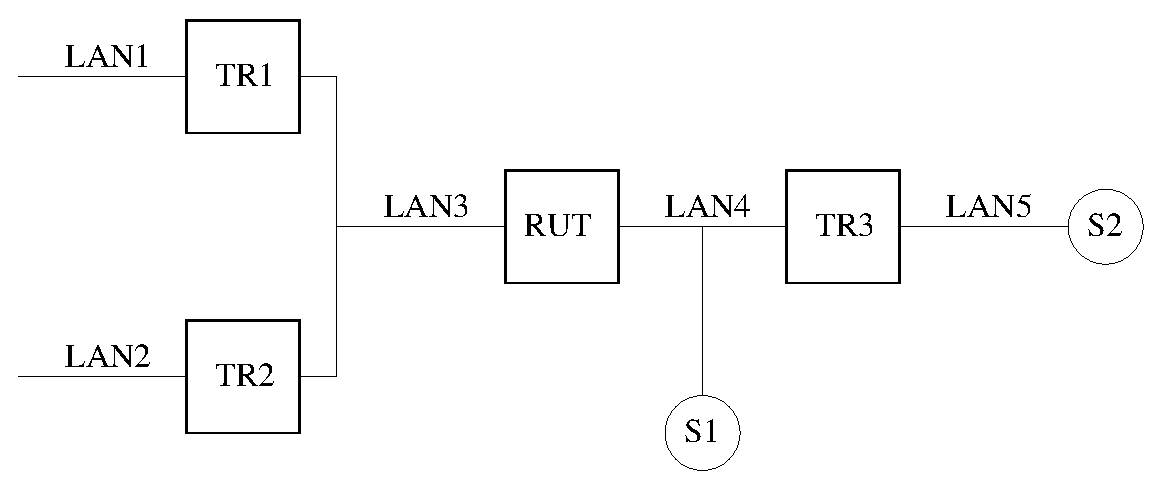
\includegraphics[scale=0.8]{figs/pim_test_4_4_receiving_sg_rpt_join_prune_messages}
    \caption{Receiving (S,G,rpt) Join/Prune messages test setup}
    \label{fig:pim_test_4_4_receiving_sg_rpt_join_prune_messages}
  \end{center}
\end{figure}

\para{Procedure:}

\subpara{Part A: Receiving (S,G,rpt) Join messages at the first-hop router.}

\begin{enumerate}

  \item Configure the RUT as the RP. Start the RUT and TR1. If
  necessary, wait until the RP-set in the RUT and TR1 converges.

  \item Start observing the downstream (S,G,rpt) per-interface state
  machine at the RUT.

  \item Compose an (S,G,rpt) Join message at TR1 with the source address set
  to the address of S1, and send it to the RUT.
  The \verb=J/P_HoldTime= of the message should be set to its default
  value ({\PimsmJPHoldTime}).

  \item Observe the downstream (S,G,rpt) per-interface state in the RUT.

  \item Start S1, and observe the data packets transmitted by the RUT on
  LAN3.

\end{enumerate}

\subpara{Part B: Receiving (S,G,rpt) Prune messages at the first-hop router.}

\begin{enumerate}

  \item Configure the RUT as the RP. Start the RUT and TR1. If
  necessary, wait until the RP-set in the RUT and TR1 converges.

  \item Start observing the downstream (S,G,rpt) per-interface state
  machine at the RUT.

  \item Compose an (S,G,rpt) Prune message at TR1 with the source address set
  to the address of S1, and send it to the RUT.
  The \verb=J/P_HoldTime= of the message should be set to its default
  value ({\PimsmJPHoldTime}).

  \item Observe the downstream (S,G,rpt) per-interface state in the RUT
  for at least \verb=J/P_HoldTime= ({\PimsmJPHoldTime}).

\end{enumerate}

\subpara{Part C: Receiving (S,G,rpt) Prune and (S,G,rpt) Join messages at the
first-hop router.}

\begin{enumerate}

  \item Configure the RUT as the RP. Start the RUT and TR1. If
  necessary, wait until the RP-set in the RUT and TR1 converges.

  \item Start observing the downstream (S,G,rpt) per-interface state
  machine at the RUT.

  \item Compose an (S,G,rpt) Prune message at TR1 with the source address set
  to the address of S1, and send it to the RUT.
  The \verb=J/P_HoldTime= of the message should be set to its default
  value ({\PimsmJPHoldTime}).

  \item Observe the downstream (S,G,rpt) per-interface state in the RUT.

  \item Start S1, and observe the data packets transmitted by the RUT on
  LAN3.

  \item Compose an (S,G,rpt) Join message at TR1 with the source address set
  to the address of S1, and send it to the RUT.
  The \verb=J/P_HoldTime= of the message should be set to its default
  value ({\PimsmJPHoldTime}).

  \item Observe the downstream (S,G,rpt) per-interface state in the RUT.

  \item Stop S1.

\end{enumerate}

\subpara{Part D: Receiving (S,G,rpt) Prune and (*,G) Join messages at the
first-hop router.}

\begin{enumerate}

  \item Configure the RUT as the RP. Start the RUT and TR1. If
  necessary, wait until the RP-set in the RUT and TR1 converges.

  \item Start observing the downstream (S,G,rpt) per-interface state
  machine at the RUT.

  \item Compose an (S,G,rpt) Prune message at TR1 with the source address set
  to the address of S1, and send it to the RUT.
  The \verb=J/P_HoldTime= of the message should be set to its default
  value ({\PimsmJPHoldTime}).

  \item Observe the downstream (S,G,rpt) per-interface state in the RUT.

  \item Start S1, and observe the data packets transmitted by the RUT on
  LAN3.

  \item Compose an (*,G) Join message at TR1 with the source address set
  to the address of S1, and send it to the RUT.
  The \verb=J/P_HoldTime= of the message should be set to its default
  value ({\PimsmJPHoldTime}).

  \item Observe the downstream (S,G,rpt) per-interface state in the RUT.

  \item Compose a message at TR1 that contains (*,G) Join with the RP
  address set to the address of the RUT, and (S,G,rpt) Prune with the source
  address set to the address of S1, and send it to the RUT.
  The \verb=J/P_HoldTime= of the message should be set to its default
  value ({\PimsmJPHoldTime}).

  \item Observe the downstream (S,G,rpt) per-interface state in the RUT.

  \item Stop S1.

\end{enumerate}

\para{Observable Results:}

\subpara{Part A:}

\begin{itemize}

  \item After the (S,G,rpt) Join message is received by the RUT,
  the (S,G,rpt) state machine for the interface that connects the RUT to
  LAN3 should continue to stay in the NoInfo state (\ie no (S,G,rpt) multicast
  routing entry should be created).

  \item After S1 is started, no multicast packets should be
  forwarded by the RUT on LAN3.

\end{itemize}

\subpara{Part B:}

\begin{itemize}

  \item After the (S,G,rpt) Prune message is received by the RUT,
  the (S,G,rpt) state machine for the interface that connects the RUT to
  LAN3 should transition to Prune-Pending state. The state machine should
  remain in that state for \verb=J/P_Override_Interval(I)=
  ({\PimsmJPOverrideIntervalI}). After that it should transition to Prune
  state:

\begin{verbatim}
Xorp> show pim join 
Group           Source          RP              Flags
224.0.1.20      10.3.0.2        10.3.0.1        SG_RPT DirectlyConnectedS 
    Upstream interface (S):    dc1
    Upstream interface (RP):   register_vif
    Upstream MRIB next hop (RP): UNKNOWN
    Upstream RPF'(S,G,rpt):    UNKNOWN
    Upstream state:            RPTNotJoined 
    Override timer:           -1
    Local receiver include WC: ................
    Joins RP:                  ................
    Joins WC:                  ................
    Prunes SG_RPT:             ......O.........
    Join state:                ................
    Prune state:               ......O.........
    Prune pending state:       ................
    Prune tmp state:           ................
    Prune pending tmp state:   ................
    Assert winner WC:          ................
    Assert lost WC:            ................
    Assert lost SG_RPT:        ................
    Could assert WC:           ................
    Could assert SG:           ................
    I am DR:                   .....OO.........
    Immediate olist RP:        ................
    Immediate olist WC:        ................
    Inherited olist SG:        ................
    Inherited olist SG_RPT:    ................
    PIM include WC:            ................
\end{verbatim}

  The Expiry Timer for the interface that connects the RUT to LAN3
  should expire after \verb=J/P_HoldTime= ({\PimsmJPHoldTime}).
  After it expires, the state machine for that interface should transition to
  NoInfo state, and the (S,G,rpt) entry itself should be removed.

\end{itemize}

\subpara{Part C:}

\begin{itemize}

  \item Until after the (S,G,rpt) Prune message is received by the RUT, the
  results should be same as in Part B.

  \item After the (S,G,rpt) Join message is received by the RUT,
  the (S,G,rpt) state machine for the interface that connects the RUT to
  LAN3 should transition to NoInfo state, and the (S,G,rpt) entry itself
  should be removed.

  \item At all time after S1 is started, no multicast packets should be
  forwarded by the RUT on LAN3.

\end{itemize}

\subpara{Part D:}

\begin{itemize}

  \item Until after the (S,G,rpt) Prune message is received by the RUT, the
  results should be same as in Part B and Part C.

  \item After S1 is started, no multicast packets should be
  forwarded by the RUT on LAN3.

  \item After the (*,G) Join message is received by the RUT,
  the (S,G,rpt) state machine for the interface that connects the RUT to
  LAN3 should transition to NoInfo state, and the (S,G,rpt) entry itself
  should be removed. However, the RUT should have created an (*,G) entry.
  The (*,G) state machine for the interface that connects the RUT to
  LAN3 should be in Join state (note that after S1 is started, the router
  would have (S,G) routing state as well because of the directly-connected
  source):

\begin{verbatim}
Xorp> show pim join 
Group           Source          RP              Flags
224.0.1.20      0.0.0.0         10.3.0.1        WC   
    Upstream interface (RP):   register_vif
    Upstream MRIB next hop (RP): UNKNOWN
    Upstream RPF'(*,G):        UNKNOWN
    Upstream state:            Joined 
    Join timer:                51
    Local receiver include WC: ................
    Joins RP:                  ................
    Joins WC:                  ......O.........
    Join state:                ......O.........
    Prune state:               ................
    Prune pending state:       ................
    I am assert winner state:  ................
    I am assert loser state:   ................
    Assert winner WC:          ................
    Assert lost WC:            ................
    Assert tracking WC:        ......O........O
    Could assert WC:           ......O.........
    I am DR:                   .....OO.........
    Immediate olist RP:        ................
    Immediate olist WC:        ......O.........
    Inherited olist SG:        ................
    Inherited olist SG_RPT:    ................
    PIM include WC:            ................
224.0.1.20      10.3.0.2        10.3.0.1        SG DirectlyConnectedS 
    Upstream interface (S):    dc1
    Upstream interface (RP):   register_vif
    Upstream MRIB next hop (RP): UNKNOWN
    Upstream MRIB next hop (S):  UNKNOWN
    Upstream RPF'(S,G):        UNKNOWN
    Upstream state:            Joined 
    Register state:            RegisterNoinfo RegisterNotCouldRegister 
    Join timer:                51
    Local receiver include WC: ................
    Local receiver include SG: ................
    Local receiver exclude SG: ................
    Joins RP:                  ................
    Joins WC:                  ......O.........
    Joins SG:                  ................
    Join state:                ................
    Prune state:               ................
    Prune pending state:       ................
    I am assert winner state:  ................
    I am assert loser state:   ................
    Assert winner WC:          ................
    Assert winner SG:          ................
    Assert lost WC:            ................
    Assert lost SG:            ................
    Assert lost SG_RPT:        ................
    Assert tracking SG:        .....OO........O
    Could assert WC:           ......O.........
    Could assert SG:           ................
    I am DR:                   .....OO.........
    Immediate olist RP:        ................
    Immediate olist WC:        ......O.........
    Immediate olist SG:        ................
    Inherited olist SG:        ......O.........
    Inherited olist SG_RPT:    ................
    PIM include WC:            ................
    PIM include SG:            ................
    PIM exclude SG:            ................
\end{verbatim}

  The multicast packets from S1 should be forwarded by the RUT on LAN3.

  \item After the message with the (*,G) Join and (S,G,rpt) Prune is received
  by the RUT, the (*,G) state machine for the interface that connects the RUT
  to LAN3 should remain in Join state, but
  the (S,G,rpt) state machine for the interface that connects the RUT to
  LAN3 should transition to Prune state:

\begin{verbatim}
Xorp> show pim join 
Group           Source          RP              Flags
224.0.1.20      0.0.0.0         10.3.0.1        WC   
    Upstream interface (RP):   register_vif
    Upstream MRIB next hop (RP): UNKNOWN
    Upstream RPF'(*,G):        UNKNOWN
    Upstream state:            Joined 
    Join timer:                28
    Local receiver include WC: ................
    Joins RP:                  ................
    Joins WC:                  ......O.........
    Join state:                ......O.........
    Prune state:               ................
    Prune pending state:       ................
    I am assert winner state:  ................
    I am assert loser state:   ................
    Assert winner WC:          ................
    Assert lost WC:            ................
    Assert tracking WC:        ......O........O
    Could assert WC:           ......O.........
    I am DR:                   .....OO.........
    Immediate olist RP:        ................
    Immediate olist WC:        ......O.........
    Inherited olist SG:        ................
    Inherited olist SG_RPT:    ................
    PIM include WC:            ................
224.0.1.20      10.3.0.2        10.3.0.1        SG_RPT DirectlyConnectedS 
    Upstream interface (S):    dc1
    Upstream interface (RP):   register_vif
    Upstream MRIB next hop (RP): UNKNOWN
    Upstream RPF'(S,G,rpt):    UNKNOWN
    Upstream state:            Pruned 
    Override timer:           -1
    Local receiver include WC: ................
    Joins RP:                  ................
    Joins WC:                  ......O.........
    Prunes SG_RPT:             ......O.........
    Join state:                ................
    Prune state:               ......O.........
    Prune pending state:       ................
    Prune tmp state:           ................
    Prune pending tmp state:   ................
    Assert winner WC:          ................
    Assert lost WC:            ................
    Assert lost SG_RPT:        ................
    Could assert WC:           ......O.........
    Could assert SG:           ................
    I am DR:                   .....OO.........
    Immediate olist RP:        ................
    Immediate olist WC:        ......O.........
    Inherited olist SG:        ................
    Inherited olist SG_RPT:    ................
    PIM include WC:            ................
224.0.1.20      10.3.0.2        10.3.0.1        SG DirectlyConnectedS 
    Upstream interface (S):    dc1
    Upstream interface (RP):   register_vif
    Upstream MRIB next hop (RP): UNKNOWN
    Upstream MRIB next hop (S):  UNKNOWN
    Upstream RPF'(S,G):        UNKNOWN
    Upstream state:            NotJoined 
    Register state:            RegisterNoinfo RegisterNotCouldRegister 
    Join timer:                -1
    Local receiver include WC: ................
    Local receiver include SG: ................
    Local receiver exclude SG: ................
    Joins RP:                  ................
    Joins WC:                  ......O.........
    Joins SG:                  ................
    Join state:                ................
    Prune state:               ................
    Prune pending state:       ................
    I am assert winner state:  ................
    I am assert loser state:   ................
    Assert winner WC:          ................
    Assert winner SG:          ................
    Assert lost WC:            ................
    Assert lost SG:            ................
    Assert lost SG_RPT:        ................
    Assert tracking SG:        ...............O
    Could assert WC:           ......O.........
    Could assert SG:           ................
    I am DR:                   .....OO.........
    Immediate olist RP:        ................
    Immediate olist WC:        ......O.........
    Immediate olist SG:        ................
    Inherited olist SG:        ................
    Inherited olist SG_RPT:    ................
    PIM include WC:            ................
    PIM include SG:            ................
    PIM exclude SG:            ................
\end{verbatim}

  The multicast packets from S1 should stop being forwarded by the RUT on
  LAN3.

\end{itemize}

\para{Possible Problems:}
None.

%%%%%%%%%%%%%%%%%%%%%%%%%%%%%%%%%%%%%%%%%%%
\newpage
\section{Sending (*,*,RP) Join/Prune Messages}

\para{Purpose:}
Verify that (*,*,RP) Join/Prune messages are sent properly.

\para{References:}
\begin{itemize}
  \item draft-ietf-pim-sm-v2-new-05 -- Section 4.5.5
\end{itemize}

\para{Discussion:}
If a router receives an (*,*,RP) Join/Prune message, it may need to propagate
it toward the RP. A router should monitor its upstream interface for messages
from other routers on that subnet, and if it sees an (*,*,RP) Join to the
correct upstream neighbor, it should suppress its own (*,*,RP) Join message.
If it sees an (*,*,RP) Prune, it should override that prune by sending an
(*,*,RP) Join almost immediately. If a router sees the Generation ID of the
correct upstream neighbor change, the router should refresh the state by
sending an (*,*,RP) Join almost immediately. In addition, if the MRIB changes
to indicate that the next hop towards the RP has changed, the router should
send an (*,*,RP) Prune towards the old next hop, and send an (*,*,RP) Join
towards the next hop router.

\para{Test Setup:}
Connect the RUT, TR1, TR2, TR3, TR4, and S1 according to
Figure~\ref{fig:pim_test_4_5_sending_rp_join_prune_messages}.
In all tests, configure the RUT such that the next-hop router toward LAN6 is
TR4, unless stated otherwise.

\begin{figure}[htbp]
  \begin{center}
    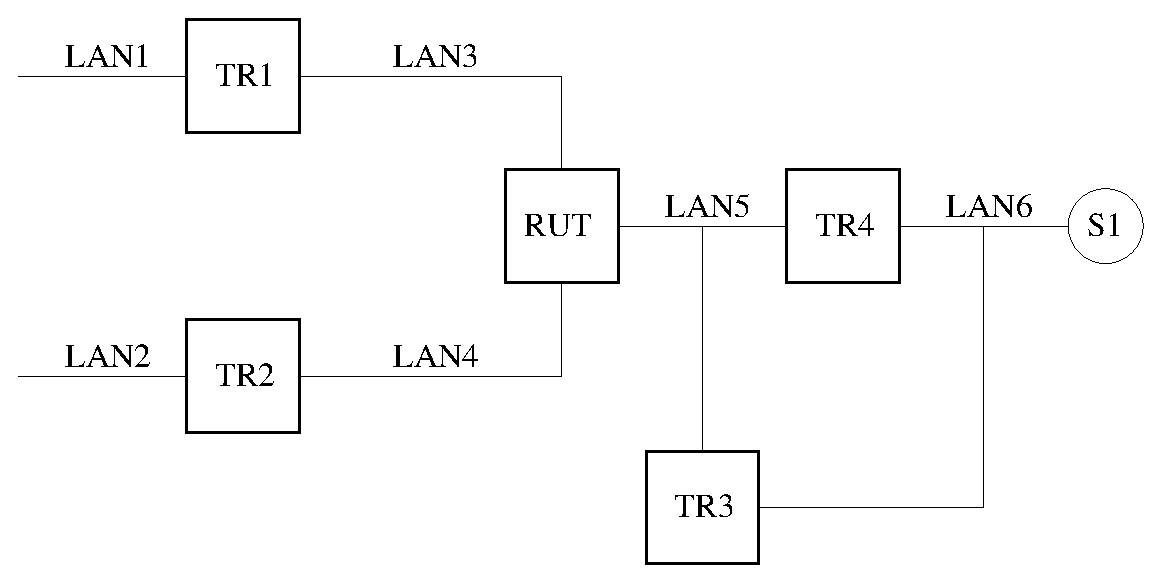
\includegraphics[scale=0.8]{figs/pim_test_4_5_sending_rp_join_prune_messages}
    \caption{Sending (*,*,RP) Join/Prune Messages test setup}
    \label{fig:pim_test_4_5_sending_rp_join_prune_messages}
  \end{center}
\end{figure}

\para{Procedure:}

\subpara{Part A: JoinDesired(*,*,RP) $\Longrightarrow$ True/False transaction.}

\begin{enumerate}

  \item Configure TR4 as the RP. Start the RUT, TR1, TR2, and TR4. If
  necessary, wait until the RP-set in the RUT, TR1, TR2, and TR4
  converges.

  \item Start observing the (*,*,RP) Join/Prune messages transmitted by the
  RUT on LAN5.

  \item Compose an (*,*,RP) Join message at TR1 with the RP address set to the
  address of TR4, and send it to the RUT. 
  The \verb=J/P_HoldTime= of the message should be set to its default
  value ({\PimsmJPHoldTime}).

  \item Compose an (*,*,RP) Prune message at TR1 with the RP address set to the
  address of TR4, and send it to the RUT. 
  The \verb=J/P_HoldTime= of the message should be set to its default
  value ({\PimsmJPHoldTime}).

  \item Compose an (*,*,RP) Join message at TR1 with the RP address set to the
  address of TR4, and send it to the RUT. 
  The \verb=J/P_HoldTime= of the message should be set to its default
  value ({\PimsmJPHoldTime}).

  \item Compose an (*,*,RP) Join message at TR2 with the RP address set to the
  address of TR4, and send it to the RUT. 
  The \verb=J/P_HoldTime= of the message should be set to its default
  value ({\PimsmJPHoldTime}).

  \item Compose an (*,*,RP) Prune message at TR2 with the RP address set to the
  address of TR4, and send it to the RUT. 
  The \verb=J/P_HoldTime= of the message should be set to its default
  value ({\PimsmJPHoldTime}).

\end{enumerate}

\subpara{Part B: (*,*,RP) Join Timer expiration.}

\begin{enumerate}

  \item Configure TR4 as the RP. Start the RUT, TR1, and TR4. If
  necessary, wait until the RP-set in the RUT, TR1, and TR4
  converges.

  \item Start observing the (*,*,RP) Join/Prune messages transmitted by the
  RUT on LAN5.

  \item Compose an (*,*,RP) Join message at TR1 with the RP address set to the
  address of TR4, and send it to the RUT. 
  The \verb=J/P_HoldTime= of the message should be set to its default
  value ({\PimsmJPHoldTime}).

  \item Keep observing the (*,*,RP) Join/Prune messages transmitted by the
  RUT on LAN5 for at least \verb=J/P_HoldTime= ({\PimsmJPHoldTime}).

\end{enumerate}

\subpara{Part C: See (*,*,RP) Join message to MRIB.next\_hop(RP).}

\begin{itemize}

  \item Configure TR4 as the RP. Start the RUT, TR1, TR3, and TR4. If
  necessary, wait until the RP-set in the RUT, TR1, TR3, and TR4
  converges.

  \item Configure the RUT such that the T-bit in LAN Prune Delay Hello
  Option in the Hello messages sent by the RUT on LAN5 is not set (\ie joins
  suppression is not disabled). The T-bit in the Hello messages of TR3 and TR4
  can be of any value.

  \item Start observing the (*,*,RP) Join/Prune messages transmitted by the
  RUT on LAN5.

  \item Compose an (*,*,RP) Join message at TR1 with the RP address set to the
  address of TR4, and send it to the RUT. 
  The \verb=J/P_HoldTime= of the message should be set to its default
  value ({\PimsmJPHoldTime}).

  \item Compose an (*,*,RP) Join message at TR3 with the RP address set to the
  address of TR4, and send it to TR4 on LAN5.
  The \verb=J/P_HoldTime= of the message should be set to its default
  value ({\PimsmJPHoldTime}).

  \item Every \verb=t_periodic= ({\PimsmTPeriodic}) compose an (*,*,RP) Join
  message at TR3 with the RP address set to the address of TR4, and send it to
  TR4 on LAN5.
  The \verb=J/P_HoldTime= of the message should be set to its default
  value ({\PimsmJPHoldTime}).

  \item Keep observing the (*,*,RP) Join/Prune messages transmitted by the
  RUT on LAN5 for at least \verb=J/P_HoldTime= ({\PimsmJPHoldTime}).

  \item Repeat the whole test, but this time by configuring the RUT, TR3, and
  TR4 such that the T-bit in LAN Prune Delay Hello Option is set (\ie joins
  suppression is disabled).

\end{itemize}

\subpara{Part D: See (*,*,RP) Prune message to MRIB.next\_hop(RP).}

\begin{itemize}

  \item Configure TR4 as the RP. Start the RUT, TR1, TR3, and TR4. If
  necessary, wait until the RP-set in the RUT, TR1, TR3, and TR4
  converges.

  \item Start observing the (*,*,RP) Join/Prune messages transmitted by the
  RUT on LAN5.

  \item Compose an (*,*,RP) Join message at TR1 with the RP address set to the
  address of TR4, and send it to the RUT. 
  The \verb=J/P_HoldTime= of the message should be set to its default
  value ({\PimsmJPHoldTime}).

  \item Compose an (*,*,RP) Prune message at TR3 with the RP address set to the
  address of TR4, and send it to TR4 on LAN5.
  The \verb=J/P_HoldTime= of the message should be set to its default
  value ({\PimsmJPHoldTime}).

  \item Keep observing the (*,*,RP) Join/Prune messages transmitted by the
  RUT on LAN5 for at least \verb=J/P_HoldTime= ({\PimsmJPHoldTime}).

\end{itemize}

\subpara{Part E: MRIB.next\_hop(RP) Changes.}

\begin{itemize}

  \item Configure the IP address of the interface that connects TR4 to LAN6 as
  the RP. Configure the RUT such that the next-hop router toward the RP is
  TR4. Start the RUT, TR1, TR3, and TR4. If necessary, wait until the
  RP-set in the RUT, TR1, TR3, and TR4 converges.

  \item Start observing the (*,*,RP) Join/Prune messages transmitted by the
  RUT on LAN5.

  \item Compose an (*,*,RP) Join message at TR1 with the RP address set to the
  RP address of TR4, and send it to the RUT. 
  The \verb=J/P_HoldTime= of the message should be set to its default
  value ({\PimsmJPHoldTime}).

  \item Change the MRIB in the RUT such that the next-hop
  router toward the RP is TR3.

  \item Keep observing the (*,*,RP) Join/Prune messages transmitted by the
  RUT on LAN5 for at least \verb=J/P_HoldTime= ({\PimsmJPHoldTime}).

\end{itemize}

\subpara{Part F: MRIB.next\_hop(RP) GenID Changes.}

\begin{itemize}

  \item Configure TR4 as the RP. Start the RUT, TR1, TR3, and TR4. If
  necessary, wait until the RP-set in the RUT, TR1, TR3, and TR4
  converges.

  \item Start observing the (*,*,RP) Join/Prune messages transmitted by the
  RUT on LAN5.

  \item Compose an (*,*,RP) Join message at TR1 with the RP address set to the
  RP address of TR4, and send it to the RUT. 
  The \verb=J/P_HoldTime= of the message should be set to its default
  value ({\PimsmJPHoldTime}).

  \item Quit TR4 (\ie stop it without graceful shutdown), and start it
  immediately.

  \item Keep observing the (*,*,RP) Join/Prune messages transmitted by the
  RUT on LAN5 for at least \verb=J/P_HoldTime= ({\PimsmJPHoldTime}).

\end{itemize}

\para{Observable Results:}

\subpara{Part A:}

\begin{itemize}

  \item After TR1 sends its first (*,*,RP) Join message to the RUT, the RUT
  itself should transmit an (*,*,RP) Join message on LAN5 with the upstream
  neighbor address set to TR4. The interface that connects the RUT to LAN3
  should be added to the set of joined interfaces for the corresponding
  (*,*,RP) routing state; the incoming interface for that state should be the
  interface that connects the RUT to LAN5:

\begin{verbatim}
Xorp> show pim join 
Group           Source          RP              Flags
224.0.0.0       10.4.0.3        10.4.0.3        RP   
    Upstream interface (RP):   dc1
    Upstream MRIB next hop (RP): 10.2.0.2
    Upstream state:            Joined 
    Join timer:                54
    Joins RP:                  ........O.....
    Join state:                ........O.....
    Prune state:               ..............
    Prune pending state:       ..............
    Could assert WC:           ........O.....
    I am DR:                   ........O.....
    Immediate olist RP:        ........O.....
    Inherited olist SG:        ..............
    Inherited olist SG_RPT:    ..............
\end{verbatim}

  \item After TR1 sends the (*,*,RP) Prune message to the RUT, the RUT itself
  should transmit an (*,*,RP) Prune message on LAN5 with the upstream neighbor
  address set to TR4. The interface that connects the RUT to LAN3 should be
  removed from the set of joined interfaces for the corresponding (*,*,RP)
  routing state; as a result, this routing state should be removed.

  \item After TR1 sends its second (*,*,RP) Join message to the RUT, the
  result should be same as when TR1 sent its first (*,*,RP) Join message.

  \item After TR2 sends the (*,*,RP) Join message to the RUT, the interface
  that connects the RUT to LAN4 should be added to the set of joined
  interfaces for the corresponding (*,*,RP) routing state; however, the RUT
  itself should not transmit an (*,*,RP) Join message as a result of that
  join:

\begin{verbatim}
Xorp> show pim join 
Group           Source          RP              Flags
224.0.0.0       10.4.0.3        10.4.0.3        RP   
    Upstream interface (RP):   dc1
    Upstream MRIB next hop (RP): 10.2.0.2
    Upstream state:            Joined 
    Join timer:                33
    Joins RP:                  ......O.O.....
    Join state:                ......O.O.....
    Prune state:               ..............
    Prune pending state:       ..............
    Could assert WC:           ......O.O.....
    I am DR:                   ........O.....
    Immediate olist RP:        ......O.O.....
    Inherited olist SG:        ..............
    Inherited olist SG_RPT:    ..............
\end{verbatim}

  \item After TR2 sends the (*,*,RP) Prune message to the RUT, the interface
  that connects the RUT to LAN4 should be removed from the set of joined
  interfaces for the corresponding (*,*,RP) routing state; however, the RUT
  itself should not transmit an (*,*,RP) Prune message as a result of that
  prune:

\begin{verbatim}
Xorp> show pim join 
Group           Source          RP              Flags
224.0.0.0       10.4.0.3        10.4.0.3        RP   
    Upstream interface (RP):   dc1
    Upstream MRIB next hop (RP): 10.2.0.2
    Upstream state:            Joined 
    Join timer:                30
    Joins RP:                  ........O.....
    Join state:                ........O.....
    Prune state:               ..............
    Prune pending state:       ..............
    Could assert WC:           ........O.....
    I am DR:                   ........O.....
    Immediate olist RP:        ........O.....
    Inherited olist SG:        ..............
    Inherited olist SG_RPT:    ..............
\end{verbatim}

\end{itemize}

\subpara{Part B:}

\begin{itemize}

  \item Until after TR1 sends the (*,*,RP) Join message, the results should be
  same as in Part A.

  \item After the RUT receives the (*,*,RP) Join message, it should start
  transmitting itself (*,*,RP) Join messages on LAN5 with the upstream
  neighbor address set to TR4: one message every \verb=t_periodic=
  ({\PimsmTPeriodic}).

\end{itemize}

\subpara{Part C:}

\begin{itemize}

  \item Until after TR1 sends the (*,*,RP) Join message, the results should be
  same as in Part A.

  \item After the RUT receives the (*,*,RP) Join message, it should
  transmit itself an (*,*,RP) Join message on LAN5 with the upstream
  neighbor address set to TR4. The Join Timer in the corresponding (*,*,RP)
  state to send the next message should be set to \verb=t_periodic=
  ({\PimsmTPeriodic}):

\begin{verbatim}
Xorp> show pim join 
Group           Source          RP              Flags
224.0.0.0       10.4.0.3        10.4.0.3        RP   
    Upstream interface (RP):   dc1
    Upstream MRIB next hop (RP): 10.2.0.2
    Upstream state:            Joined 
    Join timer:                59
    Joins RP:                  ........O.....
    Join state:                ........O.....
    Prune state:               ..............
    Prune pending state:       ..............
    Could assert WC:           ........O.....
    I am DR:                   ......O.O.....
    Immediate olist RP:        ........O.....
    Inherited olist SG:        ..............
    Inherited olist SG_RPT:    ..............
\end{verbatim}

  \item After TR3 sends the (*,*,RP) Join message to TR4, it should suppress
  the generation of the (*,*,RP) Join message at the RUT by increasing the
  Join Timer in the corresponding (*,*,RP) state to \verb=t_joinsuppress=
  (see the protocol specification for description of its value):

\begin{verbatim}
Xorp> show pim join 
Group           Source          RP              Flags
224.0.0.0       10.4.0.3        10.4.0.3        RP   
    Upstream interface (RP):   dc1
    Upstream MRIB next hop (RP): 10.2.0.2
    Upstream state:            Joined 
    Join timer:                82
    Joins RP:                  ........O.....
    Join state:                ........O.....
    Prune state:               ..............
    Prune pending state:       ..............
    Could assert WC:           ........O.....
    I am DR:                   ......O.O.....
    Immediate olist RP:        ........O.....
    Inherited olist SG:        ..............
    Inherited olist SG_RPT:    ..............
\end{verbatim}

  \item While TR3 keeps sending (*,*,RP) Join messages to TR4, the RUT should
  not generate (*,*,RP) Join messages on its own.

  \item When the test is repeated with the T-bit set, the (*,*,RP) Join
  messages sent by TR3 should not suppress the (*,*,RP) Join messages
  generated by the RUT. In other words, after the RUT receives the (*,*,RP)
  Join message, it should start transmitting itself (*,*,RP) Join messages on
  LAN5 with the upstream neighbor address set to TR4: one message every
  \verb=t_periodic= ({\PimsmTPeriodic}).

\end{itemize}

\subpara{Part D:}

\begin{itemize}

  \item Until before TR3 sends the (*,*,RP) Prune message, the results should
  be same as in Part C (right before TR3 sends the (*,*,RP) Join message).

  \item After TR3 sends the (*,*,RP) Prune message to TR4,
  the Join Timer in the RUT for the corresponding (*,*,RP) state
  should be decreased to \verb=t_override= ({\PimsmTOverride}). As a result,
  the RUT should generate almost immediately an (*,*,RP) Join message to TR4.

  \item After that the RUT should continue transmitting 
  (*,*,RP) Join messages to TR4 as normal: one message every \verb=t_periodic=
  ({\PimsmTPeriodic}).

\end{itemize}

\subpara{Part E:}

\begin{itemize}

  \item Until before the MRIB is changed, the results should
  be same as in Part C (right before TR3 sends the (*,*,RP) Join message).

  \item After the MRIB is changed, the RUT should send an (*,*,RP) Prune
  message to TR2 (the old upstream router toward the RP), and right after that
  it should send an (*,*,RP) Join message to TR3 (the new upstream router
  toward the RP). The corresponding (*,*,RP) state in the RUT should
  indicate the new upstream router, and the Join Timer should be set
  to \verb=t_periodic= ({\PimsmTPeriodic}):

\begin{verbatim}
Xorp> show pim join 
Group           Source          RP              Flags
224.0.0.0       10.4.0.3        10.4.0.3        RP   
    Upstream interface (RP):   dc1
    Upstream MRIB next hop (RP): 10.2.0.3
    Upstream state:            Joined 
    Join timer:                59
    Joins RP:                  ........O.....
    Join state:                ........O.....
    Prune state:               ..............
    Prune pending state:       ..............
    Could assert WC:           ........O.....
    I am DR:                   ......O.O.....
    Immediate olist RP:        ........O.....
    Inherited olist SG:        ..............
    Inherited olist SG_RPT:    ..............
\end{verbatim}

  \item After that the RUT should continue transmitting 
  (*,*,RP) Join messages to TR3 as normal: one message every \verb=t_periodic=
  ({\PimsmTPeriodic}).

\end{itemize}

\subpara{Part F:}

\begin{itemize}

  \item Until before TR4 is restarted, the results should
  be same as in Part C (right before TR3 sends the (*,*,RP) Join message).

  \item After TR4 is restarted,
  the Join Timer in the RUT for the corresponding (*,*,RP) state
  should be decreased to \verb=t_override= ({\PimsmTOverride}). As a result,
  the RUT should generate almost immediately an (*,*,RP) Join message to TR4.

  \item After that the RUT should continue transmitting 
  (*,*,RP) Join messages to TR4 as normal: one message every \verb=t_periodic=
  ({\PimsmTPeriodic}).

\end{itemize}


\para{Possible Problems:}
In Part E, after the MRIB is changed, the (*,*,RP) Join message might
be sent before the (*,*,RP) Prune message.

%%%%%%%%%%%%%%%%%%%%%%%%%%%%%%%%%%%%%%%%%%%
\newpage
\section{Sending (*,G) Join/Prune Messages}

\para{Purpose:}
Verify that (*,G) Join/Prune messages are sent properly.

\para{References:}
\begin{itemize}
  \item draft-ietf-pim-sm-v2-new-05 -- Section 4.5.6
\end{itemize}

\para{Discussion:}
If a router receives an (*,G) Join/Prune message, it may need to propagate
it toward the RP for that group. A router should monitor its upstream
interface for messages
from other routers on that subnet, and if it sees an (*,G) Join to the
correct upstream neighbor, it should suppress its own (*,G) Join message.
If it sees an (*,G) Prune, it should override that prune by sending an
(*,G) Join almost immediately. If a router sees the Generation ID of the
correct upstream neighbor change, the router should refresh the state by
sending an (*,G) Join almost immediately. In addition, if the MRIB changes
to indicate that the next hop towards the RP has changed, the router should
send an (*,G) Prune towards the old next hop, and send an (*,G) Join
towards the next hop router.

\para{Test Setup:}
Connect the RUT, TR1, TR2, TR3, TR4, and S1 according to
Figure~\ref{fig:pim_test_4_6_sending_wc_join_prune_messages}.
In all tests, configure the RUT such that the next-hop router toward LAN6 is
TR4, unless stated otherwise.

\begin{figure}[htbp]
  \begin{center}
    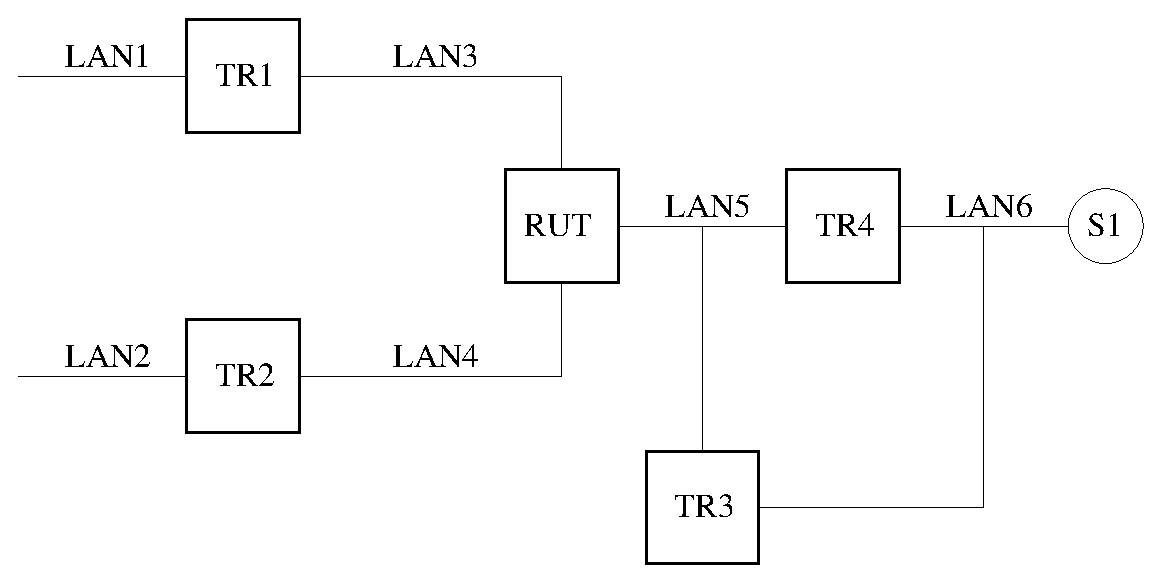
\includegraphics[scale=0.8]{figs/pim_test_4_6_sending_wc_join_prune_messages}
    \caption{Sending (*,G) Join/Prune Messages test setup}
    \label{fig:pim_test_4_6_sending_wc_join_prune_messages}
  \end{center}
\end{figure}

\para{Procedure:}

\subpara{Part A: JoinDesired(*,G) $\Longrightarrow$ True/False transaction.}

\begin{enumerate}

  \item Configure TR4 as the RP. Start the RUT, TR1, TR2, and TR4. If
  necessary, wait until the RP-set in the RUT, TR1, TR2, and TR4
  converges.

  \item Start observing the (*,G) Join/Prune messages transmitted by the
  RUT on LAN5.

  \item Compose an (*,G) Join message at TR1, and send it to the RUT. 
  The \verb=J/P_HoldTime= of the message should be set to its default
  value ({\PimsmJPHoldTime}).

  \item Compose an (*,G) Prune message at TR1, and send it to the RUT. 
  The \verb=J/P_HoldTime= of the message should be set to its default
  value ({\PimsmJPHoldTime}).

  \item Compose an (*,G) Join message at TR1, and send it to the RUT. 
  The \verb=J/P_HoldTime= of the message should be set to its default
  value ({\PimsmJPHoldTime}).

  \item Compose an (*,G) Join message at TR2, and send it to the RUT. 
  The \verb=J/P_HoldTime= of the message should be set to its default
  value ({\PimsmJPHoldTime}).

  \item Compose an (*,G) Prune message at TR2, and send it to the RUT. 
  The \verb=J/P_HoldTime= of the message should be set to its default
  value ({\PimsmJPHoldTime}).

\end{enumerate}

\subpara{Part B: (*,G) Join Timer expiration.}

\begin{enumerate}

  \item Configure TR4 as the RP. Start the RUT, TR1, and TR4. If
  necessary, wait until the RP-set in the RUT, TR1, and TR4
  converges.

  \item Start observing the (*,G) Join/Prune messages transmitted by the
  RUT on LAN5.

  \item Compose an (*,G) Join message at TR1, and send it to the RUT. 
  The \verb=J/P_HoldTime= of the message should be set to its default
  value ({\PimsmJPHoldTime}).

  \item Keep observing the (*,G) Join/Prune messages transmitted by the
  RUT on LAN5 for at least \verb=J/P_HoldTime= ({\PimsmJPHoldTime}).

\end{enumerate}

\subpara{Part C: See (*,G) Join message to RPF'(*,G).}

\begin{itemize}

  \item Configure TR4 as the RP. Start the RUT, TR1, TR3, and TR4. If
  necessary, wait until the RP-set in the RUT, TR1, TR3, and TR4
  converges.

  \item Configure the RUT such that the T-bit in LAN Prune Delay Hello
  Option in the Hello messages sent by the RUT on LAN5 is not set (\ie joins
  suppression is not disabled). The T-bit in the Hello messages of TR3 and TR4
  can be of any value.

  \item Start observing the (*,G) Join/Prune messages transmitted by the
  RUT on LAN5.

  \item Compose an (*,G) Join message at TR1, and send it to the RUT. 
  The \verb=J/P_HoldTime= of the message should be set to its default
  value ({\PimsmJPHoldTime}).

  \item Compose an (*,G) Join message at TR3, and send it to TR4 on LAN5.
  The \verb=J/P_HoldTime= of the message should be set to its default
  value ({\PimsmJPHoldTime}).

  \item Every \verb=t_periodic= ({\PimsmTPeriodic}) compose an (*,G) Join
  message at TR3, and send it to TR4 on LAN5.
  The \verb=J/P_HoldTime= of the message should be set to its default
  value ({\PimsmJPHoldTime}).

  \item Keep observing the (*,G) Join/Prune messages transmitted by the
  RUT on LAN5 for at least \verb=J/P_HoldTime= ({\PimsmJPHoldTime}).

  \item Repeat the whole test, but this time by configuring the RUT, TR3, and
  TR4 such that the T-bit in LAN Prune Delay Hello Option is set (\ie joins
  suppression is disabled).

\end{itemize}

\subpara{Part D: See (*,G) Prune message to RPF'(*,G).}

\begin{itemize}

  \item Configure TR4 as the RP. Start the RUT, TR1, TR3, and TR4. If
  necessary, wait until the RP-set in the RUT, TR1, TR3, and TR4
  converges.

  \item Start observing the (*,G) Join/Prune messages transmitted by the
  RUT on LAN5.

  \item Compose an (*,G) Join message at TR1, and send it to the RUT. 
  The \verb=J/P_HoldTime= of the message should be set to its default
  value ({\PimsmJPHoldTime}).

  \item Compose an (*,G) Prune message at TR3, and send it to TR4 on LAN5.
  The \verb=J/P_HoldTime= of the message should be set to its default
  value ({\PimsmJPHoldTime}).

  \item Keep observing the (*,G) Join/Prune messages transmitted by the
  RUT on LAN5 for at least \verb=J/P_HoldTime= ({\PimsmJPHoldTime}).

\end{itemize}

\subpara{Part E: MRIB.next\_hop(RP(G)) Changes.}

\begin{itemize}

  \item Configure the IP address of the interface that connects TR4 to LAN6 as
  the RP. Configure the RUT such that the next-hop router toward the RP is
  TR4. Start the RUT, TR1, TR3, and TR4. If necessary, wait until the
  RP-set in the RUT, TR1, TR3, and TR4 converges.

  \item Start observing the (*,G) Join/Prune messages transmitted by the
  RUT on LAN5.

  \item Compose an (*,G) Join message at TR1, and send it to the RUT. 
  The \verb=J/P_HoldTime= of the message should be set to its default
  value ({\PimsmJPHoldTime}).

  \item Change the MRIB in the RUT such that the next-hop
  router toward the RP is TR3.

  \item Keep observing the (*,G) Join/Prune messages transmitted by the
  RUT on LAN5 for at least \verb=J/P_HoldTime= ({\PimsmJPHoldTime}).

\end{itemize}

\subpara{Part F: RPF'(*,G) GenID Changes.}

\begin{itemize}

  \item Configure TR4 as the RP. Start the RUT, TR1, TR3, and TR4. If
  necessary, wait until the RP-set in the RUT, TR1, TR3, and TR4
  converges.

  \item Start observing the (*,G) Join/Prune messages transmitted by the
  RUT on LAN5.

  \item Compose an (*,G) Join message at TR1, and send it to the RUT. 
  The \verb=J/P_HoldTime= of the message should be set to its default
  value ({\PimsmJPHoldTime}).

  \item Quit TR4 (\ie stop it without graceful shutdown), and start it
  immediately.

  \item Keep observing the (*,G) Join/Prune messages transmitted by the
  RUT on LAN5 for at least \verb=J/P_HoldTime= ({\PimsmJPHoldTime}).

\end{itemize}

\subpara{Part G: RPF'(*,G) Changes.}

\begin{itemize}

  \item Configure the IP address of the interface that connects TR4 to LAN6 as
  the RP. Configure the RUT such that the next-hop router toward the RP is
  TR4. Start the RUT, TR1, TR3, and TR4. If necessary, wait until the
  RP-set in the RUT, TR1, TR3, and TR4 converges.

  \item Start observing the (*,G) Join/Prune messages transmitted by the
  RUT on LAN5.

  \item Compose an (*,G) Join message at TR1, and send it to the RUT. 
  The \verb=J/P_HoldTime= of the message should be set to its default
  value ({\PimsmJPHoldTime}).

  \item Trigger changing of RPF'(*,G) at the RUT to TR3 by composing an
  (*,G) Assert message at TR3 with RPT-bit set to one, metric and metric 
  preference set to zero, and sending it on LAN5.

  \item Keep observing the (*,G) Join/Prune messages transmitted by the
  RUT on LAN5 for at least \verb=J/P_HoldTime= ({\PimsmJPHoldTime}).

\end{itemize}

\para{Observable Results:}

\subpara{Part A:}

\begin{itemize}

  \item After TR1 sends its first (*,G) Join message to the RUT, the RUT
  itself should transmit an (*,G) Join message on LAN5 with the upstream
  neighbor address set to TR4. The interface that connects the RUT to LAN3
  should be added to the set of joined interfaces for the corresponding
  (*,G) routing state; the incoming interface for that state should be the
  interface that connects the RUT to LAN5:

\begin{verbatim}
Xorp> show pim join
Group           Source          RP              Flags
224.0.1.20      0.0.0.0         10.4.0.3        WC   
    Upstream interface (RP):   dc1
    Upstream MRIB next hop (RP): 10.2.0.2
    Upstream RPF'(*,G):        10.2.0.2
    Upstream state:            Joined 
    Join timer:                52
    Local receiver include WC: ..............
    Joins RP:                  ..............
    Joins WC:                  ........O.....
    Join state:                ........O.....
    Prune state:               ..............
    Prune pending state:       ..............
    I am assert winner state:  ..............
    I am assert loser state:   ..............
    Assert winner WC:          ..............
    Assert lost WC:            ..............
    Assert tracking WC:        .....O..O.....
    Could assert WC:           ........O.....
    I am DR:                   ........O.....
    Immediate olist RP:        ..............
    Immediate olist WC:        ........O.....
    Inherited olist SG:        ..............
    Inherited olist SG_RPT:    ..............
    PIM include WC:            ..............
\end{verbatim}

  \item After TR1 sends the (*,G) Prune message to the RUT, the RUT itself
  should transmit an (*,G) Prune message on LAN5 with the upstream neighbor
  address set to TR4. The interface that connects the RUT to LAN3 should be
  removed from the set of joined interfaces for the corresponding (*,G)
  routing state; as a result, this routing state should be removed.

  \item After TR1 sends its second (*,G) Join message to the RUT, the
  result should be same as when TR1 sent its first (*,G) Join message.

  \item After TR2 sends the (*,G) Join message to the RUT, the interface
  that connects the RUT to LAN4 should be added to the set of joined
  interfaces for the corresponding (*,G) routing state; however, the RUT
  itself should not transmit an (*,G) Join message as a result of that
  join:

\begin{verbatim}
Xorp> show pim join
Group           Source          RP              Flags
224.0.1.20      0.0.0.0         10.4.0.3        WC   
    Upstream interface (RP):   dc1
    Upstream MRIB next hop (RP): 10.2.0.2
    Upstream RPF'(*,G):        10.2.0.2
    Upstream state:            Joined 
    Join timer:                6
    Local receiver include WC: ..............
    Joins RP:                  ..............
    Joins WC:                  ......O.O.....
    Join state:                ......O.O.....
    Prune state:               ..............
    Prune pending state:       ..............
    I am assert winner state:  ..............
    I am assert loser state:   ..............
    Assert winner WC:          ..............
    Assert lost WC:            ..............
    Assert tracking WC:        .....OO.O.....
    Could assert WC:           ......O.O.....
    I am DR:                   ........O.....
    Immediate olist RP:        ..............
    Immediate olist WC:        ......O.O.....
    Inherited olist SG:        ..............
    Inherited olist SG_RPT:    ..............
    PIM include WC:            ..............
\end{verbatim}

  \item After TR2 sends the (*,G) Prune message to the RUT, the interface
  that connects the RUT to LAN4 should be removed from the set of joined
  interfaces for the corresponding (*,G) routing state; however, the RUT
  itself should not transmit an (*,G) Prune message as a result of that
  prune:

\begin{verbatim}
Xorp> show pim join
Group           Source          RP              Flags
224.0.1.20      0.0.0.0         10.4.0.3        WC   
    Upstream interface (RP):   dc1
    Upstream MRIB next hop (RP): 10.2.0.2
    Upstream RPF'(*,G):        10.2.0.2
    Upstream state:            Joined 
    Join timer:                4
    Local receiver include WC: ..............
    Joins RP:                  ..............
    Joins WC:                  ........O.....
    Join state:                ........O.....
    Prune state:               ..............
    Prune pending state:       ..............
    I am assert winner state:  ..............
    I am assert loser state:   ..............
    Assert winner WC:          ..............
    Assert lost WC:            ..............
    Assert tracking WC:        .....O..O.....
    Could assert WC:           ........O.....
    I am DR:                   ........O.....
    Immediate olist RP:        ..............
    Immediate olist WC:        ........O.....
    Inherited olist SG:        ..............
    Inherited olist SG_RPT:    ..............
    PIM include WC:            ..............
\end{verbatim}

\end{itemize}

\subpara{Part B:}

\begin{itemize}

  \item Until after TR1 sends the (*,G) Join message, the results should be
  same as in Part A.

  \item After the RUT receives the (*,G) Join message, it should start
  transmitting itself (*,G) Join messages on LAN5 with the upstream
  neighbor address set to TR4: one message every \verb=t_periodic=
  ({\PimsmTPeriodic}).

\end{itemize}

\subpara{Part C:}

\begin{itemize}

  \item Until after TR1 sends the (*,G) Join message, the results should be
  same as in Part A.

  \item After the RUT receives the (*,G) Join message, it should
  transmit itself an (*,G) Join message on LAN5 with the upstream
  neighbor address set to TR4. The Join Timer in the corresponding (*,G)
  state to send the next message should be set to \verb=t_periodic=
  ({\PimsmTPeriodic}):

\begin{verbatim}
Xorp> show pim join 
Group           Source          RP              Flags
224.0.1.20      0.0.0.0         10.4.0.3        WC   
    Upstream interface (RP):   dc1
    Upstream MRIB next hop (RP): 10.2.0.2
    Upstream RPF'(*,G):        10.2.0.2
    Upstream state:            Joined 
    Join timer:                58
    Local receiver include WC: ..............
    Joins RP:                  ..............
    Joins WC:                  ........O.....
    Join state:                ........O.....
    Prune state:               ..............
    Prune pending state:       ..............
    I am assert winner state:  ..............
    I am assert loser state:   ..............
    Assert winner WC:          ..............
    Assert lost WC:            ..............
    Assert tracking WC:        .....O..O.....
    Could assert WC:           ........O.....
    I am DR:                   ........O.....
    Immediate olist RP:        ..............
    Immediate olist WC:        ........O.....
    Inherited olist SG:        ..............
    Inherited olist SG_RPT:    ..............
    PIM include WC:            ..............
\end{verbatim}

  \item After TR3 sends the (*,G) Join message to TR4, it should suppress
  the generation of the (*,G) Join message at the RUT by increasing the
  Join Timer in the corresponding (*,G) state to \verb=t_joinsuppress=
  (see the protocol specification for description of its value):

\begin{verbatim}
Xorp> show pim join 
Group           Source          RP              Flags
224.0.1.20      0.0.0.0         10.4.0.3        WC   
    Upstream interface (RP):   dc1
    Upstream MRIB next hop (RP): 10.2.0.2
    Upstream RPF'(*,G):        10.2.0.2
    Upstream state:            Joined 
    Join timer:                81
    Local receiver include WC: ..............
    Joins RP:                  ..............
    Joins WC:                  ........O.....
    Join state:                ........O.....
    Prune state:               ..............
    Prune pending state:       ..............
    I am assert winner state:  ..............
    I am assert loser state:   ..............
    Assert winner WC:          ..............
    Assert lost WC:            ..............
    Assert tracking WC:        .....O..O.....
    Could assert WC:           ........O.....
    I am DR:                   ........O.....
    Immediate olist RP:        ..............
    Immediate olist WC:        ........O.....
    Inherited olist SG:        ..............
    Inherited olist SG_RPT:    ..............
    PIM include WC:            ..............
\end{verbatim}

  \item While TR3 keeps sending (*,G) Join messages to TR4, the RUT should
  not generate (*,G) Join messages on its own.

  \item When the test is repeated with the T-bit set, the (*,G) Join
  messages sent by TR3 should not suppress the (*,G) Join messages
  generated by the RUT. In other words, after the RUT receives the (*,G)
  Join message, it should start transmitting itself (*,G) Join messages on
  LAN5 with the upstream neighbor address set to TR4: one message every
  \verb=t_periodic= ({\PimsmTPeriodic}).

\end{itemize}

\subpara{Part D:}

\begin{itemize}

  \item Until before TR3 sends the (*,G) Prune message, the results should
  be same as in Part C (right before TR3 sends the (*,G) Join message).

  \item After TR3 sends the (*,G) Prune message to TR4,
  the Join Timer in the RUT for the corresponding (*,G) state
  should be decreased to \verb=t_override= ({\PimsmTOverride}). As a result,
  the RUT should generate almost immediately an (*,G) Join message to TR4.

  \item After that the RUT should continue transmitting 
  (*,G) Join messages to TR4 as normal: one message every \verb=t_periodic=
  ({\PimsmTPeriodic}).

\end{itemize}

\subpara{Part E:}

\begin{itemize}

  \item Until before the MRIB is changed, the results should
  be same as in Part C (right before TR3 sends the (*,G) Join message).

  \item After the MRIB is changed, the RUT should send an (*,G) Prune
  message to TR2 (the old upstream router toward the RP), and right after that
  it should send an (*,G) Join message to TR3 (the new upstream router
  toward the RP). The corresponding (*,G) state in the RUT should
  indicate the new upstream router, and the Join Timer should be set
  to \verb=t_periodic= ({\PimsmTPeriodic}):

\begin{verbatim}
Xorp> show pim join 
Group           Source          RP              Flags
224.0.1.20      0.0.0.0         10.4.0.3        WC   
    Upstream interface (RP):   dc1
    Upstream MRIB next hop (RP): 10.2.0.3
    Upstream RPF'(*,G):        10.2.0.3
    Upstream state:            Joined 
    Join timer:                56
    Local receiver include WC: ..............
    Joins RP:                  ..............
    Joins WC:                  ........O.....
    Join state:                ........O.....
    Prune state:               ..............
    Prune pending state:       ..............
    I am assert winner state:  ..............
    I am assert loser state:   ..............
    Assert winner WC:          ..............
    Assert lost WC:            ..............
    Assert tracking WC:        .....O..O.....
    Could assert WC:           ........O.....
    I am DR:                   ........O.....
    Immediate olist RP:        ..............
    Immediate olist WC:        ........O.....
    Inherited olist SG:        ..............
    Inherited olist SG_RPT:    ..............
    PIM include WC:            ..............
\end{verbatim}

  \item After that the RUT should continue transmitting 
  (*,G) Join messages to TR3 as normal: one message every \verb=t_periodic=
  ({\PimsmTPeriodic}).

\end{itemize}

\subpara{Part F:}

\begin{itemize}

  \item Until before TR4 is restarted, the results should
  be same as in Part C (right before TR3 sends the (*,G) Join message).

  \item After TR4 is restarted,
  the Join Timer in the RUT for the corresponding (*,G) state
  should be decreased to \verb=t_override= ({\PimsmTOverride}). As a result,
  the RUT should generate almost immediately an (*,G) Join message to TR4.

  \item After that the RUT should continue transmitting 
  (*,G) Join messages to TR4 as normal: one message every \verb=t_periodic=
  ({\PimsmTPeriodic}).

\end{itemize}

\subpara{Part G:}

\begin{itemize}

  \item Until before RPF'(*,G) is changed, the results should
  be same as in Part C (right before TR3 sends the (*,G) Join message).

  \item After RPF'(*,G) is changed,
  the Join Timer in the RUT for the corresponding (*,G) state
  should be decreased to \verb=t_override= ({\PimsmTOverride}). As a result,
  the RUT should generate almost immediately an (*,G) Join message to TR3.
  The RPF'(*,G) for the corresponding (*,G) state should be set to TR3:

\begin{verbatim}
Xorp> show pim join
Group           Source          RP              Flags
224.0.1.20      0.0.0.0         10.4.0.3        WC   
    Upstream interface (RP):   dc1
    Upstream MRIB next hop (RP): 10.2.0.2
    Upstream RPF'(*,G):        10.2.0.3
    Upstream state:            Joined 
    Join timer:                58
    Local receiver include WC: ..............
    Joins RP:                  ..............
    Joins WC:                  ........O.....
    Join state:                ........O.....
    Prune state:               ..............
    Prune pending state:       ..............
    I am assert winner state:  ..............
    I am assert loser state:   .....O........
    Assert winner WC:          ..............
    Assert lost WC:            ..............
    Assert tracking WC:        .....O..O.....
    Could assert WC:           ........O.....
    I am DR:                   ......O.O.....
    Immediate olist RP:        ..............
    Immediate olist WC:        ........O.....
    Inherited olist SG:        ..............
    Inherited olist SG_RPT:    ..............
    PIM include WC:            ..............
\end{verbatim}

  \item After that the RUT should continue transmitting 
  (*,G) Join messages to TR3 as normal: one message every \verb=t_periodic=
  ({\PimsmTPeriodic}).

\end{itemize}


\para{Possible Problems:}
In Part E, after the MRIB is changed, the (*,G) Join message might
be sent before the (*,G) Prune message. In Part G, if the Assert generated by
TR3 is not preferred when compared to the assert metric of TR4, the RPF'(*,G)
in the RUT will not be changed.

%%%%%%%%%%%%%%%%%%%%%%%%%%%%%%%%%%%%%%%%%%%
\newpage
\section{Sending (S,G) Join/Prune Messages}

\para{Purpose:}
Verify that (S,G) Join/Prune messages are sent properly.

\para{References:}
\begin{itemize}
  \item draft-ietf-pim-sm-v2-new-05 -- Section 4.5.7
\end{itemize}

\para{Discussion:}
If a router receives an (S,G) Join/Prune message, it may need to propagate
it toward the source. A router should monitor its upstream
interface for messages
from other routers on that subnet, and if it sees an (S,G) Join to the
correct upstream neighbor, it should suppress its own (S,G) Join message.
If it sees an (S,G) Prune, it should override that prune by sending an
(S,G) Join almost immediately. If a router sees the Generation ID of the
correct upstream neighbor change, the router should refresh the state by
sending an (S,G) Join almost immediately. In addition, if the MRIB changes
to indicate that the next hop towards the source has changed, the router should
send an (S,G) Prune towards the old next hop, and send an (S,G) Join
towards the next hop router.

\para{Test Setup:}
Connect the RUT, TR1, TR2, TR3, TR4, and S1 according to
Figure~\ref{fig:pim_test_4_7_sending_sg_join_prune_messages}.
In all tests, configure the RUT such that the next-hop router toward LAN6 is
TR4, unless stated otherwise.

\begin{figure}[htbp]
  \begin{center}
    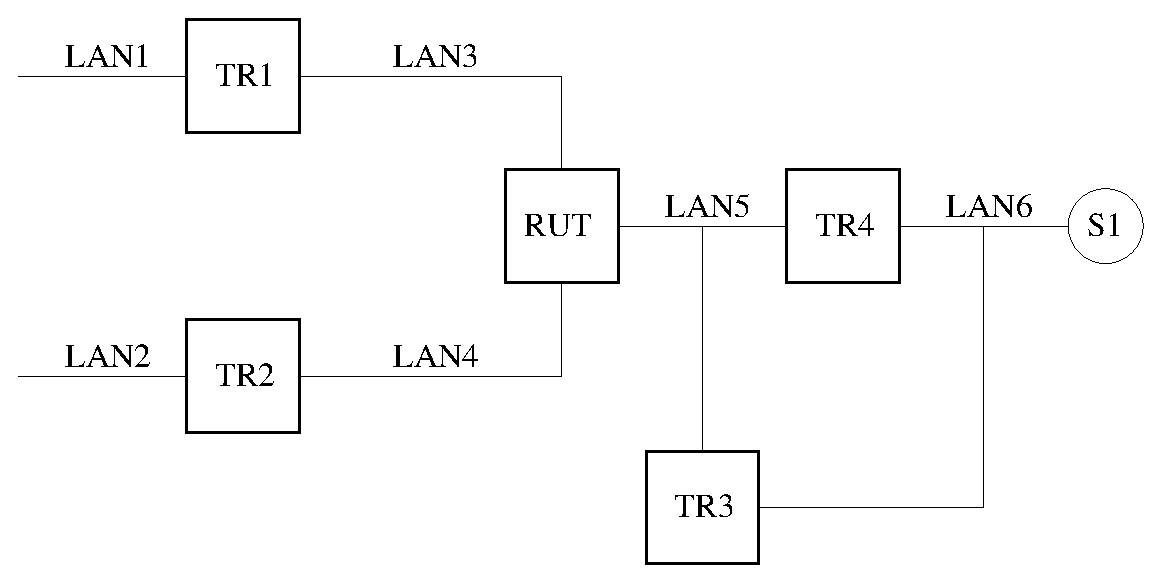
\includegraphics[scale=0.8]{figs/pim_test_4_7_sending_sg_join_prune_messages}
    \caption{Sending (S,G) Join/Prune Messages test setup}
    \label{fig:pim_test_4_7_sending_sg_join_prune_messages}
  \end{center}
\end{figure}

\para{Procedure:}

\subpara{Part A: JoinDesired(S,G) $\Longrightarrow$ True/False transaction.}

\begin{enumerate}

  \item Configure TR4 as the RP. Start the RUT, TR1, TR2, and TR4. If
  necessary, wait until the RP-set in the RUT, TR1, TR2, and TR4
  converges.

  \item Start observing the (S,G) Join/Prune messages transmitted by the
  RUT on LAN5.

  \item Compose an (S,G) Join message at TR1 with the S address set to the
  address of S1, and send it to the RUT. 
  The \verb=J/P_HoldTime= of the message should be set to its default
  value ({\PimsmJPHoldTime}).

  \item Compose an (S,G) Prune message at TR1 with the S address set to the
  address of S1, and send it to the RUT. 
  The \verb=J/P_HoldTime= of the message should be set to its default
  value ({\PimsmJPHoldTime}).

  \item Compose an (S,G) Join message at TR1 with the S address set to the
  address of S1, and send it to the RUT. 
  The \verb=J/P_HoldTime= of the message should be set to its default
  value ({\PimsmJPHoldTime}).

  \item Compose an (S,G) Join message at TR2 with the S address set to the
  address of S1, and send it to the RUT. 
  The \verb=J/P_HoldTime= of the message should be set to its default
  value ({\PimsmJPHoldTime}).

  \item Compose an (S,G) Prune message at TR2 with the S address set to the
  address of S1, and send it to the RUT. 
  The \verb=J/P_HoldTime= of the message should be set to its default
  value ({\PimsmJPHoldTime}).

\end{enumerate}

\subpara{Part B: (S,G) Join Timer expiration.}

\begin{enumerate}

  \item Configure TR4 as the RP. Start the RUT, TR1, and TR4. If
  necessary, wait until the RP-set in the RUT, TR1, and TR4
  converges.

  \item Start observing the (S,G) Join/Prune messages transmitted by the
  RUT on LAN5.

  \item Compose an (S,G) Join message at TR1 with the S address set to the
  address of S1, and send it to the RUT. 
  The \verb=J/P_HoldTime= of the message should be set to its default
  value ({\PimsmJPHoldTime}).

  \item Keep observing the (S,G) Join/Prune messages transmitted by the
  RUT on LAN5 for at least \verb=J/P_HoldTime= ({\PimsmJPHoldTime}).

\end{enumerate}

\subpara{Part C: See (S,G) Join message to RPF'(S,G).}

\begin{itemize}

  \item Configure TR4 as the RP. Start the RUT, TR1, TR3, and TR4. If
  necessary, wait until the RP-set in the RUT, TR1, TR3, and TR4
  converges.

  \item Configure the RUT such that the T-bit in LAN Prune Delay Hello
  Option in the Hello messages sent by the RUT on LAN5 is not set (\ie joins
  suppression is not disabled). The T-bit in the Hello messages of TR3 and TR4
  can be of any value.

  \item Start observing the (S,G) Join/Prune messages transmitted by the
  RUT on LAN5.

  \item Compose an (S,G) Join message at TR1 with the S address set to the
  address of S1, and send it to the RUT. 
  The \verb=J/P_HoldTime= of the message should be set to its default
  value ({\PimsmJPHoldTime}).

  \item Compose an (S,G) Join message at TR3 with the S address set to the
  address of S1, and send it to TR4 on LAN5.
  The \verb=J/P_HoldTime= of the message should be set to its default
  value ({\PimsmJPHoldTime}).

  \item Every \verb=t_periodic= ({\PimsmTPeriodic}) compose an (S,G) Join
  message at TR3 with the S address set to the address of S1, and send it to
  TR4 on LAN5.
  The \verb=J/P_HoldTime= of the message should be set to its default
  value ({\PimsmJPHoldTime}).

  \item Keep observing the (S,G) Join/Prune messages transmitted by the
  RUT on LAN5 for at least \verb=J/P_HoldTime= ({\PimsmJPHoldTime}).

  \item Repeat the whole test, but this time by configuring the RUT, TR3, and
  TR4 such that the T-bit in LAN Prune Delay Hello Option is set (\ie joins
  suppression is disabled).

\end{itemize}

\subpara{Part D: See (S,G) Prune message to RPF'(S,G).}

\begin{itemize}

  \item Configure TR4 as the RP. Start the RUT, TR1, TR3, and TR4. If
  necessary, wait until the RP-set in the RUT, TR1, TR3, and TR4
  converges.

  \item Start observing the (S,G) Join/Prune messages transmitted by the
  RUT on LAN5.

  \item Compose an (S,G) Join message at TR1 with the S address set to the
  address of S1, and send it to the RUT. 
  The \verb=J/P_HoldTime= of the message should be set to its default
  value ({\PimsmJPHoldTime}).

  \item Compose an (S,G) Prune message at TR3 with the S address set to the
  address of S1, and send it to TR4 on LAN5.
  The \verb=J/P_HoldTime= of the message should be set to its default
  value ({\PimsmJPHoldTime}).

  \item Keep observing the (S,G) Join/Prune messages transmitted by the
  RUT on LAN5 for at least \verb=J/P_HoldTime= ({\PimsmJPHoldTime}).

\end{itemize}

\subpara{Part E: MRIB.next\_hop(S) Changes.}

\begin{itemize}

  \item Configure TR4 as the RP.
  Configure the RUT such that the next-hop router toward S1 is TR4.
  Start the RUT, TR1, TR3, and TR4.
  If necessary, wait until the RP-set in the RUT, TR1, TR3, and TR4
  converges.

  \item Start observing the (S,G) Join/Prune messages transmitted by the
  RUT on LAN5.

  \item Compose an (S,G) Join message at TR1 with the S address set to the
  address of S1, and send it to the RUT. 
  The \verb=J/P_HoldTime= of the message should be set to its default
  value ({\PimsmJPHoldTime}).

  \item Change the MRIB in the RUT such that the next-hop
  router toward S1 is TR3.

  \item Keep observing the (S,G) Join/Prune messages transmitted by the
  RUT on LAN5 for at least \verb=J/P_HoldTime= ({\PimsmJPHoldTime}).

\end{itemize}

\subpara{Part F: RPF'(S,G) GenID Changes.}

\begin{itemize}

  \item Configure TR4 as the RP. Start the RUT, TR1, TR3, and TR4. If
  necessary, wait until the RP-set in the RUT, TR1, TR3, and TR4
  converges.

  \item Start observing the (S,G) Join/Prune messages transmitted by the
  RUT on LAN5.

  \item Compose an (S,G) Join message at TR1 with the S address set to the
  address of S1, and send it to the RUT. 
  The \verb=J/P_HoldTime= of the message should be set to its default
  value ({\PimsmJPHoldTime}).

  \item Quit TR4 (\ie stop it without graceful shutdown), and start it
  immediately.

  \item Keep observing the (S,G) Join/Prune messages transmitted by the
  RUT on LAN5 for at least \verb=J/P_HoldTime= ({\PimsmJPHoldTime}).

\end{itemize}

\subpara{Part G: RPF'(S,G) Changes.}

\begin{itemize}

  \item Configure TR4 as the RP.
  Configure the RUT such that the next-hop router toward S1 is TR4.
  Start the RUT, TR1, TR3, and TR4.
  If necessary, wait until the RP-set in the RUT, TR1, TR3, and TR4
  converges.

  \item Start observing the (S,G) Join/Prune messages transmitted by the
  RUT on LAN5.

  \item Compose an (S,G) Join message at TR1 with the S address set to the
  address of S1, and send it to the RUT. 
  The \verb=J/P_HoldTime= of the message should be set to its default
  value ({\PimsmJPHoldTime}).

  \item Trigger changing of RPF'(S,G) at the RUT to TR3 by composing an
  (S,G) Assert message at TR3 with RPT-bit, metric and metric 
  preference set to zero, and sending it on LAN5.

  \item Keep observing the (S,G) Join/Prune messages transmitted by the
  RUT on LAN5 for at least \verb=J/P_HoldTime= ({\PimsmJPHoldTime}).

\end{itemize}

\subpara{Part H: See (S,G,rpt) Prune message to RPF'(S,G).}

This part is same as Part D, except that TR3 sends to TR4 (S,G,rpt) Prune
instead of (S,G) Prune.

\subpara{Part I: See (*,G) Prune message to RPF'(S,G).}

This part is same as Part D, except that TR3 sends to TR4 (*,G) Prune
instead of (S,G) Prune.

\para{Observable Results:}

\subpara{Part A:}

\begin{itemize}

  \item After TR1 sends its first (S,G) Join message to the RUT, the RUT
  itself should transmit an (S,G) Join message on LAN5 with the upstream
  neighbor address set to TR4. The interface that connects the RUT to LAN3
  should be added to the set of joined interfaces for the corresponding
  (S,G) routing state; the incoming interface for that state should be the
  interface that connects the RUT to LAN5:

\begin{verbatim}
Xorp> show pim join 
Group           Source          RP              Flags
224.0.1.20      10.4.0.2        10.4.0.3        SG   
    Upstream interface (S):    dc1
    Upstream interface (RP):   dc1
    Upstream MRIB next hop (RP): 10.2.0.2
    Upstream MRIB next hop (S):  10.2.0.2
    Upstream RPF'(S,G):        10.2.0.2
    Upstream state:            Joined 
    Join timer:                53
    Local receiver include WC: ..............
    Local receiver include SG: ..............
    Local receiver exclude SG: ..............
    Joins RP:                  ..............
    Joins WC:                  ..............
    Joins SG:                  ........O.....
    Join state:                ........O.....
    Prune state:               ..............
    Prune pending state:       ..............
    I am assert winner state:  ..............
    I am assert loser state:   ..............
    Assert winner WC:          ..............
    Assert winner SG:          ..............
    Assert lost WC:            ..............
    Assert lost SG:            ..............
    Assert lost SG_RPT:        ..............
    Assert tracking SG:        .....O..O.....
    Could assert WC:           ..............
    Could assert SG:           ..............
    I am DR:                   ......O.O.....
    Immediate olist RP:        ..............
    Immediate olist WC:        ..............
    Immediate olist SG:        ........O.....
    Inherited olist SG:        ........O.....
    Inherited olist SG_RPT:    ..............
    PIM include WC:            ..............
    PIM include SG:            ..............
    PIM exclude SG:            ..............
\end{verbatim}

  \item After TR1 sends the (S,G) Prune message to the RUT, the RUT itself
  should transmit an (S,G) Prune message on LAN5 with the upstream neighbor
  address set to TR4. The interface that connects the RUT to LAN3 should be
  removed from the set of joined interfaces for the corresponding (S,G)
  routing state; as a result, this routing state should be removed.

  \item After TR1 sends its second (S,G) Join message to the RUT, the
  result should be same as when TR1 sent its first (S,G) Join message.

  \item After TR2 sends the (S,G) Join message to the RUT, the interface
  that connects the RUT to LAN4 should be added to the set of joined
  interfaces for the corresponding (S,G) routing state; however, the RUT
  itself should not transmit an (S,G) Join message as a result of that
  join:

\begin{verbatim}
Xorp> show pim join 
Group           Source          RP              Flags
224.0.1.20      10.4.0.2        10.4.0.3        SG   
    Upstream interface (S):    dc1
    Upstream interface (RP):   dc1
    Upstream MRIB next hop (RP): 10.2.0.2
    Upstream MRIB next hop (S):  10.2.0.2
    Upstream RPF'(S,G):        10.2.0.2
    Upstream state:            Joined 
    Join timer:                2
    Local receiver include WC: ..............
    Local receiver include SG: ..............
    Local receiver exclude SG: ..............
    Joins RP:                  ..............
    Joins WC:                  ..............
    Joins SG:                  ......O.O.....
    Join state:                ......O.O.....
    Prune state:               ..............
    Prune pending state:       ..............
    I am assert winner state:  ..............
    I am assert loser state:   ..............
    Assert winner WC:          ..............
    Assert winner SG:          ..............
    Assert lost WC:            ..............
    Assert lost SG:            ..............
    Assert lost SG_RPT:        ..............
    Assert tracking SG:        .....OO.O.....
    Could assert WC:           ..............
    Could assert SG:           ..............
    I am DR:                   ........O.....
    Immediate olist RP:        ..............
    Immediate olist WC:        ..............
    Immediate olist SG:        ......O.O.....
    Inherited olist SG:        ......O.O.....
    Inherited olist SG_RPT:    ..............
    PIM include WC:            ..............
    PIM include SG:            ..............
    PIM exclude SG:            ..............
\end{verbatim}

  \item After TR2 sends the (S,G) Prune message to the RUT, the interface
  that connects the RUT to LAN4 should be removed from the set of joined
  interfaces for the corresponding (S,G) routing state; however, the RUT
  itself should not transmit an (S,G) Prune message as a result of that
  prune:

\begin{verbatim}
Xorp> show pim join 
Group           Source          RP              Flags
224.0.1.20      10.4.0.2        10.4.0.3        SG   
    Upstream interface (S):    dc1
    Upstream interface (RP):   dc1
    Upstream MRIB next hop (RP): 10.2.0.2
    Upstream MRIB next hop (S):  10.2.0.2
    Upstream RPF'(S,G):        10.2.0.2
    Upstream state:            Joined 
    Join timer:                3
    Local receiver include WC: ..............
    Local receiver include SG: ..............
    Local receiver exclude SG: ..............
    Joins RP:                  ..............
    Joins WC:                  ..............
    Joins SG:                  ........O.....
    Join state:                ........O.....
    Prune state:               ..............
    Prune pending state:       ..............
    I am assert winner state:  ..............
    I am assert loser state:   ..............
    Assert winner WC:          ..............
    Assert winner SG:          ..............
    Assert lost WC:            ..............
    Assert lost SG:            ..............
    Assert lost SG_RPT:        ..............
    Assert tracking SG:        .....O..O.....
    Could assert WC:           ..............
    Could assert SG:           ..............
    I am DR:                   ........O.....
    Immediate olist RP:        ..............
    Immediate olist WC:        ..............
    Immediate olist SG:        ........O.....
    Inherited olist SG:        ........O.....
    Inherited olist SG_RPT:    ..............
    PIM include WC:            ..............
    PIM include SG:            ..............
    PIM exclude SG:            ..............
\end{verbatim}

\end{itemize}

\subpara{Part B:}

\begin{itemize}

  \item Until after TR1 sends the (S,G) Join message, the results should be
  same as in Part A.

  \item After the RUT receives the (S,G) Join message, it should start
  transmitting itself (S,G) Join messages on LAN5 with the upstream
  neighbor address set to TR4: one message every \verb=t_periodic=
  ({\PimsmTPeriodic}).

\end{itemize}

\subpara{Part C:}

\begin{itemize}

  \item Until after TR1 sends the (S,G) Join message, the results should be
  same as in Part A.

  \item After the RUT receives the (S,G) Join message, it should
  transmit itself an (S,G) Join message on LAN5 with the upstream
  neighbor address set to TR4. The Join Timer in the corresponding (S,G)
  state to send the next message should be set to \verb=t_periodic=
  ({\PimsmTPeriodic}):

\begin{verbatim}
Xorp> show pim join 
Group           Source          RP              Flags
224.0.1.20      10.4.0.2        10.4.0.3        SG   
    Upstream interface (S):    dc1
    Upstream interface (RP):   dc1
    Upstream MRIB next hop (RP): 10.2.0.2
    Upstream MRIB next hop (S):  10.2.0.2
    Upstream RPF'(S,G):        10.2.0.2
    Upstream state:            Joined 
    Join timer:                56
    Local receiver include WC: ..............
    Local receiver include SG: ..............
    Local receiver exclude SG: ..............
    Joins RP:                  ..............
    Joins WC:                  ..............
    Joins SG:                  ........O.....
    Join state:                ........O.....
    Prune state:               ..............
    Prune pending state:       ..............
    I am assert winner state:  ..............
    I am assert loser state:   ..............
    Assert winner WC:          ..............
    Assert winner SG:          ..............
    Assert lost WC:            ..............
    Assert lost SG:            ..............
    Assert lost SG_RPT:        ..............
    Assert tracking SG:        .....O..O.....
    Could assert WC:           ..............
    Could assert SG:           ..............
    I am DR:                   ........O.....
    Immediate olist RP:        ..............
    Immediate olist WC:        ..............
    Immediate olist SG:        ........O.....
    Inherited olist SG:        ........O.....
    Inherited olist SG_RPT:    ..............
    PIM include WC:            ..............
    PIM include SG:            ..............
    PIM exclude SG:            ..............
\end{verbatim}

  \item After TR3 sends the (S,G) Join message to TR4, it should suppress
  the generation of the (S,G) Join message at the RUT by increasing the
  Join Timer in the corresponding (S,G) entry to \verb=t_joinsuppress=
  (see the protocol specification for description of its value):

\begin{verbatim}
Xorp> show pim join 
Group           Source          RP              Flags
224.0.1.20      10.4.0.2        10.4.0.3        SG   
    Upstream interface (S):    dc1
    Upstream interface (RP):   dc1
    Upstream MRIB next hop (RP): 10.2.0.2
    Upstream MRIB next hop (S):  10.2.0.2
    Upstream RPF'(S,G):        10.2.0.2
    Upstream state:            Joined 
    Join timer:                75
    Local receiver include WC: ..............
    Local receiver include SG: ..............
    Local receiver exclude SG: ..............
    Joins RP:                  ..............
    Joins WC:                  ..............
    Joins SG:                  ........O.....
    Join state:                ........O.....
    Prune state:               ..............
    Prune pending state:       ..............
    I am assert winner state:  ..............
    I am assert loser state:   ..............
    Assert winner WC:          ..............
    Assert winner SG:          ..............
    Assert lost WC:            ..............
    Assert lost SG:            ..............
    Assert lost SG_RPT:        ..............
    Assert tracking SG:        .....O..O.....
    Could assert WC:           ..............
    Could assert SG:           ..............
    I am DR:                   ........O.....
    Immediate olist RP:        ..............
    Immediate olist WC:        ..............
    Immediate olist SG:        ........O.....
    Inherited olist SG:        ........O.....
    Inherited olist SG_RPT:    ..............
    PIM include WC:            ..............
    PIM include SG:            ..............
    PIM exclude SG:            ..............
\end{verbatim}

  \item While TR3 keeps sending (S,G) Join messages to TR4, the RUT should
  not generate (S,G) Join messages on its own.

  \item When the test is repeated with the T-bit set, the (S,G) Join
  messages sent by TR3 should not suppress the (S,G) Join messages
  generated by the RUT. In other words, after the RUT receives the (S,G)
  Join message, it should start transmitting itself (S,G) Join messages on
  LAN5 with the upstream neighbor address set to TR4: one message every
  \verb=t_periodic= ({\PimsmTPeriodic}).

\end{itemize}

\subpara{Part D:}

\begin{itemize}

  \item Until before TR3 sends the (S,G) Prune message, the results should
  be same as in Part C (right before TR3 sends the (S,G) Join message).

  \item After TR3 sends the (S,G) Prune message to TR4,
  the Join Timer in the RUT for the corresponding (S,G) state
  should be decreased to \verb=t_override= ({\PimsmTOverride}). As a result,
  the RUT should generate almost immediately an (S,G) Join message to TR4.

  \item After that the RUT should continue transmitting 
  (S,G) Join messages to TR4 as normal: one message every \verb=t_periodic=
  ({\PimsmTPeriodic}).

\end{itemize}

\subpara{Part E:}

\begin{itemize}

  \item Until before the MRIB is changed, the results should
  be same as in Part C (right before TR3 sends the (S,G) Join message).

  \item After the MRIB is changed, the RUT should send an (S,G) Prune
  message to TR2 (the old upstream router toward the RP), and right after that
  it should send an (S,G) Join message to TR3 (the new upstream router
  toward the RP). The corresponding (S,G) state in the RUT should
  indicate the new upstream router, and the Join Timer should be set
  to \verb=t_periodic= ({\PimsmTPeriodic}):

\begin{verbatim}
Xorp> show pim join 
Group           Source          RP              Flags
224.0.1.20      10.4.0.2        10.4.0.3        SG   
    Upstream interface (S):    dc1
    Upstream interface (RP):   dc1
    Upstream MRIB next hop (RP): 10.2.0.3
    Upstream MRIB next hop (S):  10.2.0.3
    Upstream RPF'(S,G):        10.2.0.3
    Upstream state:            Joined 
    Join timer:                53
    Local receiver include WC: ..............
    Local receiver include SG: ..............
    Local receiver exclude SG: ..............
    Joins RP:                  ..............
    Joins WC:                  ..............
    Joins SG:                  ........O.....
    Join state:                ........O.....
    Prune state:               ..............
    Prune pending state:       ..............
    I am assert winner state:  ..............
    I am assert loser state:   ..............
    Assert winner WC:          ..............
    Assert winner SG:          ..............
    Assert lost WC:            ..............
    Assert lost SG:            ..............
    Assert lost SG_RPT:        ..............
    Assert tracking SG:        .....O..O.....
    Could assert WC:           ..............
    Could assert SG:           ..............
    I am DR:                   ........O.....
    Immediate olist RP:        ..............
    Immediate olist WC:        ..............
    Immediate olist SG:        ........O.....
    Inherited olist SG:        ........O.....
    Inherited olist SG_RPT:    ..............
    PIM include WC:            ..............
    PIM include SG:            ..............
    PIM exclude SG:            ..............
\end{verbatim}

  \item After that the RUT should continue transmitting 
  (S,G) Join messages to TR3 as normal: one message every \verb=t_periodic=
  ({\PimsmTPeriodic}).

\end{itemize}

\subpara{Part F:}

\begin{itemize}

  \item Until before TR4 is restarted, the results should
  be same as in Part C (right before TR3 sends the (S,G) Join message).

  \item After TR4 is restarted,
  the Join Timer in the RUT for the corresponding (S,G) state
  should be decreased to \verb=t_override= ({\PimsmTOverride}). As a result,
  the RUT should generate almost immediately an (S,G) Join message to TR4.

  \item After that the RUT should continue transmitting 
  (S,G) Join messages to TR4 as normal: one message every \verb=t_periodic=
  ({\PimsmTPeriodic}).

\end{itemize}

\subpara{Part G:}

\begin{itemize}

  \item Until before RPF'(S,G) is changed, the results should
  be same as in Part C (right before TR3 sends the (S,G) Join message).

  \item After RPF'(S,G) is changed,
  the Join Timer in the RUT for the corresponding (S,G) state
  should be decreased to \verb=t_override= ({\PimsmTOverride}). As a result,
  the RUT should generate almost immediately an (S,G) Join message to TR3.
  The RPF'(*,G) for the corresponding (*,G) state should be set to TR3:

\begin{verbatim}
Xorp> show pim join
Group           Source          RP              Flags
224.0.1.20      10.4.0.2        10.4.0.3        SG SPT 
    Upstream interface (S):    dc1
    Upstream interface (RP):   dc1
    Upstream MRIB next hop (RP): 10.2.0.2
    Upstream MRIB next hop (S):  10.2.0.2
    Upstream RPF'(S,G):        10.2.0.3
    Upstream state:            Joined 
    Join timer:                49
    Local receiver include WC: ..............
    Local receiver include SG: ..............
    Local receiver exclude SG: ..............
    Joins RP:                  ..............
    Joins WC:                  ..............
    Joins SG:                  ........O.....
    Join state:                ........O.....
    Prune state:               ..............
    Prune pending state:       ..............
    I am assert winner state:  ..............
    I am assert loser state:   .....O........
    Assert winner WC:          ..............
    Assert winner SG:          ..............
    Assert lost WC:            ..............
    Assert lost SG:            ..............
    Assert lost SG_RPT:        ..............
    Assert tracking SG:        .....O..O.....
    Could assert WC:           ..............
    Could assert SG:           ........O.....
    I am DR:                   ......O.O.....
    Immediate olist RP:        ..............
    Immediate olist WC:        ..............
    Immediate olist SG:        ........O.....
    Inherited olist SG:        ........O.....
    Inherited olist SG_RPT:    ..............
    PIM include WC:            ..............
    PIM include SG:            ..............
    PIM exclude SG:            ..............
\end{verbatim}

  \item After that the RUT should continue transmitting 
  (S,G) Join messages to TR3 as normal: one message every \verb=t_periodic=
  ({\PimsmTPeriodic}).

\end{itemize}

\subpara{Part H:}

\begin{itemize}

  \item Until before TR3 sends the (S,G) Prune message, the results should
  be same as in Part C (right before TR3 sends the (S,G) Join message).

  \item After TR3 sends the (S,G,rpt) Prune message to TR4,
  the Join Timer in the RUT for the corresponding (S,G) state
  should be decreased to \verb=t_override= ({\PimsmTOverride}). As a result,
  the RUT should generate almost immediately an (S,G) Join message to TR4.

  \item After that the RUT should continue transmitting 
  (S,G) Join messages to TR4 as normal: one message every \verb=t_periodic=
  ({\PimsmTPeriodic}).

\end{itemize}

\subpara{Part I:}

\begin{itemize}

  \item Until before TR3 sends the (S,G) Prune message, the results should
  be same as in Part C (right before TR3 sends the (S,G) Join message).

  \item After TR3 sends the (*,G) Prune message to TR4,
  the Join Timer in the RUT for the corresponding (S,G) state
  should be decreased to \verb=t_override= ({\PimsmTOverride}). As a result,
  the RUT should generate almost immediately an (S,G) Join message to TR4.

  \item After that the RUT should continue transmitting 
  (S,G) Join messages to TR4 as normal: one message every \verb=t_periodic=
  ({\PimsmTPeriodic}).

\end{itemize}


\para{Possible Problems:}
In Part E, after the MRIB is changed, the (S,G) Join message might
be sent before the (S,G) Prune message. In Part G, if the Assert generated by
TR3 is not preferred when compared to the assert metric of TR4, the RPF'(S,G)
in the RUT will not be changed.

%%%%%%%%%%%%%%%%%%%%%%%%%%%%%%%%%%%%%%%%%%%
\newpage
\section{(S,G,rpt) Periodic Messages}

\para{Purpose:}
Verify that (S,G,rpt) Prune periodic messages are sent properly.

\para{References:}
\begin{itemize}
  \item draft-ietf-pim-sm-v2-new-05 -- Section 4.5.8
\end{itemize}

\para{Discussion:}
When a router is going to send a Join (*,G) message, it may need to include a
Prune (S,G,rpt) in the compound Join/Prune message for each (S,G) it has
state.

\para{Test Setup:}
Connect the RUT, TR1, TR2, TR3, TR4, and S1 according to
Figure~\ref{fig:pim_test_4_8_sg_rpt_periodic_messages}.
Configure the IP address of the interface that connects TR4 to LAN6 as the RP.
Configure the RUT such that the next-hop router toward the RP is TR2.
Configure TR3 such that the next-hop router toward S1 is TR4.

\begin{figure}[htbp]
  \begin{center}
    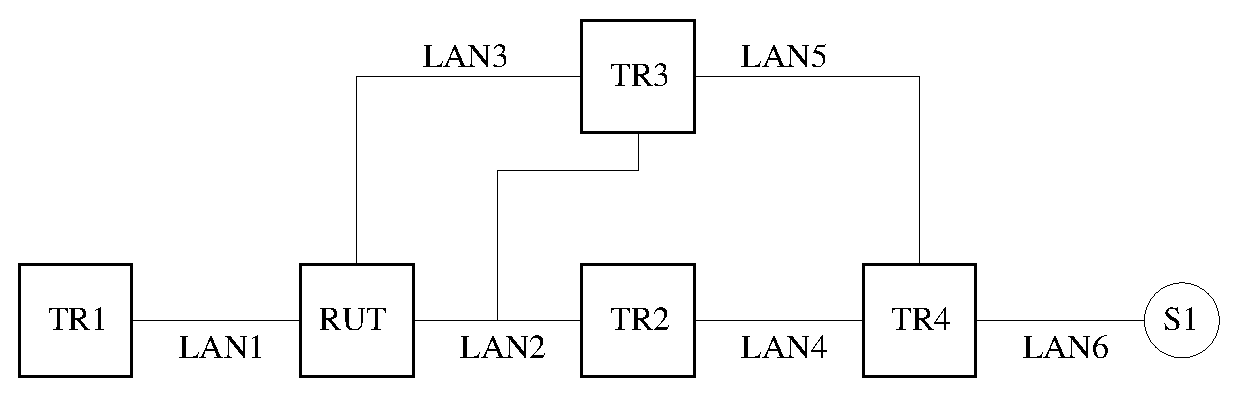
\includegraphics[scale=0.8]{figs/pim_test_4_8_sg_rpt_periodic_messages}
    \caption{(S,G,rpt) periodic messages test setup}
    \label{fig:pim_test_4_8_sg_rpt_periodic_messages}
  \end{center}
\end{figure}

\para{Procedure:}

\subpara{Part A: SPTbit(S,G) == TRUE.}

\begin{enumerate}

  \item Configure the RUT such that the next hop router toward S1 is
  TR2. Start the RUT, TR1, TR2, TR3, and TR4. If necessary, wait until the
  RP-set in the RUT, TR1, TR2, TR3, and TR4 converges.

  \item Start observing the Join/Prune messages transmitted by the RUT on
  LAN2.

  \item Compose an (*,G) Join message at TR1, and send it to the RUT. 
  The \verb=J/P_HoldTime= of the message should be set to its default
  value ({\PimsmJPHoldTime}).

  \item Compose an (S,G) Join message at TR1 with the S address set to the
  address of S1, and send it to the RUT. 
  The \verb=J/P_HoldTime= of the message should be set to its default
  value ({\PimsmJPHoldTime}).

  \item Start S1.

  \item Keep observing the Join/Prune messages transmitted by the
  RUT on LAN2 until the next (*,G) Join message is transmitted on
  LAN2 (\ie for at least \verb=t_periodic= ({\PimsmTPeriodic})).

  \item Change the MRIB in the RUT such that the next-hop
  router toward S1 is the interface that connects TR3 to LAN3.

  \item Keep observing the Join/Prune messages transmitted by the
  RUT on LAN2 until the next (*,G) Join message is transmitted on
  LAN2 (\ie for at least \verb=t_periodic= ({\PimsmTPeriodic})).

  \item Change the MRIB in the RUT such that the next-hop router
  router toward S1 is TR2.

  \item Keep observing the Join/Prune messages transmitted by the
  RUT on LAN2 until the next (*,G) Join message is transmitted on
  LAN2 (\ie for at least \verb=t_periodic= ({\PimsmTPeriodic})).

  \item Repeat the whole test, except that this time change the MRIB in the
  RUT such that the next-hop router toward S1 is the interface that connects
  TR3 to LAN2.

\end{enumerate}

\subpara{Part B: SPTbit(S,G) != TRUE AND inherited\_olist(S,G,rpt) == NULL.}

\begin{enumerate}

  \item Configure the RUT such that the next hop router toward S1 is
  TR2. Start the RUT, TR1, TR2, and TR4. If necessary, wait until the
  RP-set in the RUT, TR1, TR2, and TR4 converges.

  \item Start observing the Join/Prune messages transmitted by the RUT on
  LAN2.

  \item Compose an (*,G) Join message at TR1, and send it to the RUT. 
  The \verb=J/P_HoldTime= of the message should be set to its default
  value ({\PimsmJPHoldTime}).

  \item Compose an (S,G,rpt) Prune message at TR1 with the S address set to the
  address of S1, and send it to the RUT. 
  The \verb=J/P_HoldTime= of the message should be set to its default
  value ({\PimsmJPHoldTime}).

  \item Keep observing the Join/Prune messages transmitted by the
  RUT on LAN2 until the next (*,G) Join message is transmitted on
  LAN2 (\ie for at least \verb=t_periodic= ({\PimsmTPeriodic})).

  \item Compose an (S,G,rpt) Join message at TR1 with the S address set to the
  address of S1, and send it to the RUT. 
  The \verb=J/P_HoldTime= of the message should be set to its default
  value ({\PimsmJPHoldTime}).

  \item Keep observing the Join/Prune messages transmitted by the
  RUT on LAN2 until the next (*,G) Join message is transmitted on
  LAN2 (\ie for at least \verb=t_periodic= ({\PimsmTPeriodic})).

\end{enumerate}

\subpara{Part C: SPTbit(S,G) != TRUE AND inherited\_olist(S,G,rpt) != NULL
  AND RPF'(*,G) != RPF'(S,G,rpt).}

\begin{enumerate}

  \item Configure the RUT such that the next hop router toward S1 is
  TR2. Start the RUT, TR1, TR2, TR3, and TR4. If necessary, wait until the
  RP-set in the RUT, TR1, TR2, TR3, and TR4 converges.

  \item Start observing the Join/Prune messages transmitted by the RUT on
  LAN2.

  \item Compose an (*,G) Join message at TR1, and send it to the RUT. 
  The \verb=J/P_HoldTime= of the message should be set to its default
  value ({\PimsmJPHoldTime}).

  \item Trigger changing of RPF'(S,G,rpt) at the RUT to TR3 by composing an
  (S,G) Assert message at TR3 with RPT-bit, metric and metric 
  preference set to zero, and sending it on LAN2.

  \item Keep observing the Join/Prune messages transmitted by the
  RUT on LAN2 until the next (*,G) Join message is transmitted on
  LAN2 (\ie for at least \verb=t_periodic= ({\PimsmTPeriodic})).

  \item Trigger changing of RPF'(S,G,rpt) at the RUT to TR2 by composing an
  (S,G) Assert message at TR3 with RPT-bit set to zero, metric and metric 
  preference set to 10000, and sending it on LAN2. Right after that
  compose an (S,G) Assert message at TR2 with RPT-bit, metric and metric 
  preference set to zero, and send it on LAN2.

  \item Keep observing the Join/Prune messages transmitted by the
  RUT on LAN2 until the next (*,G) Join message is transmitted on
  LAN2 (\ie for at least \verb=t_periodic= ({\PimsmTPeriodic})).

\end{enumerate}

\para{Observable Results:}

\subpara{Part A:}

\begin{itemize}

  \item After TR1 sends the (*,G) Join message to the RUT, the RUT
  itself should transmit an (*,G) Join message on LAN2 with the upstream
  neighbor address set to TR2. The interface that connects the RUT to LAN1
  should be added to the set of joined interfaces for the corresponding
  (*,G) routing state; the incoming interface for that state should be the
  interface that connects the RUT to LAN2. The results for the (S,G) Join
  message should be similar:

\begin{verbatim}
Xorp> show pim join 
Group           Source          RP              Flags
224.0.1.20      0.0.0.0         10.4.0.1        WC   
    Upstream interface (RP):   dc1
    Upstream MRIB next hop (RP): 10.2.0.2
    Upstream RPF'(*,G):        10.2.0.2
    Upstream state:            Joined 
    Join timer:                13
    Local receiver include WC: ..............
    Joins RP:                  ..............
    Joins WC:                  ........O.....
    Join state:                ........O.....
    Prune state:               ..............
    Prune pending state:       ..............
    I am assert winner state:  ..............
    I am assert loser state:   ..............
    Assert winner WC:          ..............
    Assert lost WC:            ..............
    Assert tracking WC:        .....O..O.....
    Could assert WC:           ........O.....
    I am DR:                   ........O.....
    Immediate olist RP:        ..............
    Immediate olist WC:        ........O.....
    Inherited olist SG:        ..............
    Inherited olist SG_RPT:    ..............
    PIM include WC:            ..............
224.0.1.20      10.4.0.2        10.4.0.1        SG   
    Upstream interface (S):    dc1
    Upstream interface (RP):   dc1
    Upstream MRIB next hop (RP): 10.2.0.2
    Upstream MRIB next hop (S):  10.2.0.2
    Upstream RPF'(S,G):        10.2.0.2
    Upstream state:            Joined 
    Join timer:                40
    Local receiver include WC: ..............
    Local receiver include SG: ..............
    Local receiver exclude SG: ..............
    Joins RP:                  ..............
    Joins WC:                  ........O.....
    Joins SG:                  ........O.....
    Join state:                ........O.....
    Prune state:               ..............
    Prune pending state:       ..............
    I am assert winner state:  ..............
    I am assert loser state:   ..............
    Assert winner WC:          ..............
    Assert winner SG:          ..............
    Assert lost WC:            ..............
    Assert lost SG:            ..............
    Assert lost SG_RPT:        ..............
    Assert tracking SG:        .....O..O.....
    Could assert WC:           ........O.....
    Could assert SG:           ..............
    I am DR:                   ........O.....
    Immediate olist RP:        ..............
    Immediate olist WC:        ........O.....
    Immediate olist SG:        ........O.....
    Inherited olist SG:        ........O.....
    Inherited olist SG_RPT:    ..............
    PIM include WC:            ..............
    PIM include SG:            ..............
    PIM exclude SG:            ..............
\end{verbatim}

  \item After S1 is started, the SPT bit for the (S,G) routing state should be
  set:

\begin{verbatim}
Xorp> show pim join 
<del>
224.0.1.20      10.4.0.2        10.4.0.1        SG SPT 
<del>
\end{verbatim}

  \item Before the MRIB in the RUT is changed, the periodic (*,G) Join
  messages sent by the RUT on LAN2 to neighbor TR2, may contain (S,G) Join
  inside, but it must not contain (S,G,rpt) Prune.

  \item After the MRIB in the RUT is changed for first time, the periodic
  (*,G) Join messages sent by the RUT on LAN2 to neighbor TR2 must contain
  (S,G,rpt) Prune as well.

  \item After the MRIB in the RUT is changed for second time, the periodic
  (*,G) Join messages sent by the RUT on LAN2 to neighbor TR2 must not contain
  (S,G,rpt) Prune.

  \item When the test is repeated such that the MRIB in the RUT is changed so
  the next-hop router toward S1 is the interface that connects TR3 to LAN2,
  the results should be same.

\end{itemize}

\subpara{Part B:}

\begin{itemize}

  \item Until after TR1 sends the (*,G) Join message, the results should be
  same as in Part A.

  \item After the RUT receives the (S,G,rpt) Prune message, it should send
  (S,G,rpt) Prune message on LAN2 with the upstream neighbor address set to
  TR2. In addition to the (*,G) entry, the RUT must contain also
  (S,G,rpt) entry that is in Pruned state:

\begin{verbatim}
Xorp> show pim join 
Group           Source          RP              Flags
224.0.1.20      0.0.0.0         10.4.0.1        WC   
<del>
224.0.1.20      10.4.0.2        10.4.0.1        SG_RPT 
    Upstream interface (S):    dc1
    Upstream interface (RP):   dc1
    Upstream MRIB next hop (RP): 10.2.0.2
    Upstream RPF'(S,G,rpt):    10.2.0.2
    Upstream state:            Pruned 
    Override timer:           -1
    Local receiver include WC: ..............
    Joins RP:                  ..............
    Joins WC:                  ........O.....
    Prunes SG_RPT:             ........O.....
    Join state:                ..............
    Prune state:               ........O.....
    Prune pending state:       ..............
    Prune tmp state:           ..............
    Prune pending tmp state:   ..............
    Assert winner WC:          ..............
    Assert lost WC:            ..............
    Could assert WC:           ..............
    Could assert SG:           ..............
    I am DR:                   ........O.....
    Immediate olist RP:        ..............
    Immediate olist WC:        ........O.....
    Inherited olist SG:        ..............
    Inherited olist SG_RPT:    ..............
    PIM include WC:            ..............
\end{verbatim}

  Until before the (S,G,rpt) Join is received, the periodic (*,G) Join messages
  sent by the RUT on LAN2 to neighbor TR2 must contain (S,G,rpt) Prune as
  well.

  \item After the (S,G,rpt) Join is received, the RUT must send (S,G,rpt) Join
  message on LAN2 to neighbor TR2, and the (S,G,rpt) entry should be removed
  (if it is not removed, it must be in Not Pruned state).
  Further, the periodic (*,G) Join messages sent by the RUT on LAN2 to
  neighbor TR2 must not contain (S,G,rpt) Prune anymore.

\end{itemize}

\subpara{Part C:}

\begin{itemize}

  \item Until after TR1 sends the (*,G) Join message, the results should be
  same as in Part A.

  \item After the RPF'(S,G,rpt) at the RUT is changed by the (S,G) Assert
  message transmitted by TR3 on LAN2, the RUT must send
  (S,G,rpt) Prune message on LAN2 with the upstream neighbor address set to
  TR2. In addition to the (*,G) entry, the RUT must contain also an (S,G,rpt)
  entry that is in Pruned state, and an (S,G) entry that contains the Assert
  information:

\begin{verbatim}
Xorp> show pim join 
Group           Source          RP              Flags
224.0.1.20      0.0.0.0         10.4.0.1        WC   
<del>
224.0.1.20      10.4.0.2        10.4.0.1        SG_RPT 
    Upstream interface (S):    dc1
    Upstream interface (RP):   dc1
    Upstream MRIB next hop (RP): 10.2.0.2
    Upstream RPF'(S,G,rpt):    10.2.0.4
    Upstream state:            Pruned 
    Override timer:           -1
    Local receiver include WC: ..............
    Joins RP:                  ..............
    Joins WC:                  ........O.....
    Prunes SG_RPT:             ..............
    Join state:                ..............
    Prune state:               ..............
    Prune pending state:       ..............
    Prune tmp state:           ..............
    Prune pending tmp state:   ..............
    Assert winner WC:          ..............
    Assert lost WC:            ..............
    Assert lost SG_RPT:        ..............
    Could assert WC:           ........O.....
    Could assert SG:           ........O.....
    I am DR:                   ........O.....
    Immediate olist RP:        ..............
    Immediate olist WC:        ........O.....
    Inherited olist SG:        ..............
    Inherited olist SG_RPT:    ........O.....
    PIM include WC:            ..............
224.0.1.20      10.4.0.2        10.4.0.1        SG SPT 
    Upstream interface (S):    dc1
    Upstream interface (RP):   dc1
    Upstream MRIB next hop (RP): 10.2.0.2
    Upstream MRIB next hop (S):  10.2.0.2
    Upstream RPF'(S,G):        10.2.0.4
    Upstream state:            NotJoined 
    Join timer:                -1
    Local receiver include WC: ..............
    Local receiver include SG: ..............
    Local receiver exclude SG: ..............
    Joins RP:                  ..............
    Joins WC:                  ........O.....
    Joins SG:                  ..............
    Join state:                ..............
    Prune state:               ..............
    Prune pending state:       ..............
    I am assert winner state:  ..............
    I am assert loser state:   .....O........
    Assert winner WC:          ..............
    Assert winner SG:          ..............
    Assert lost WC:            ..............
    Assert lost SG:            ..............
    Assert lost SG_RPT:        ..............
    Assert tracking SG:        ........O.....
    Could assert WC:           ........O.....
    Could assert SG:           ........O.....
    I am DR:                   ........O.....
    Immediate olist RP:        ..............
    Immediate olist WC:        ........O.....
    Immediate olist SG:        ..............
    Inherited olist SG:        ........O.....
    Inherited olist SG_RPT:    ..............
    PIM include WC:            ..............
    PIM include SG:            ..............
    PIM exclude SG:            ..............
\end{verbatim}

  Until before the RPF'(S,G,rpt) at the RUT is changed back to TR2, the
  periodic (*,G) Join messages sent by the RUT on LAN2 to neighbor TR2
  must contain (S,G,rpt) Prune as well.

  \item Right after the RPF'(S,G,rpt) at the RUT is changed back to TR2 as a
  result of the second and third Assert messages sent by TR3 and TR2 on LAN2,
  the RUT must send an (S,G,rpt) Join message on LAN2 with the upstream
  neighbor address set to TR2. The (S,G,rpt) entry at the RUT may be removed,
  but the (S,G) entry must be kept until the new Assert state expires, and it
  must indicate that RPF'(S,G) has changed back to TR2:

\begin{verbatim}
Xorp> show pim join 
224.0.1.20      10.4.0.2        10.4.0.1        SG SPT 
    Upstream interface (S):    dc1
    Upstream interface (RP):   dc1
    Upstream MRIB next hop (RP): 10.2.0.2
    Upstream MRIB next hop (S):  10.2.0.2
    Upstream RPF'(S,G):        10.2.0.2
    Upstream state:            NotJoined 
    Join timer:                -1
    Local receiver include WC: ..............
    Local receiver include SG: ..............
    Local receiver exclude SG: ..............
    Joins RP:                  ..............
    Joins WC:                  ........O.....
    Joins SG:                  ..............
    Join state:                ..............
    Prune state:               ..............
    Prune pending state:       ..............
    I am assert winner state:  ..............
    I am assert loser state:   .....O........
    Assert winner WC:          ..............
    Assert winner SG:          ..............
    Assert lost WC:            ..............
    Assert lost SG:            ..............
    Assert lost SG_RPT:        ..............
    Assert tracking SG:        ........O.....
    Could assert WC:           ........O.....
    Could assert SG:           ........O.....
    I am DR:                   ........O.....
    Immediate olist RP:        ..............
    Immediate olist WC:        ........O.....
    Immediate olist SG:        ..............
    Inherited olist SG:        ........O.....
    Inherited olist SG_RPT:    ..............
    PIM include WC:            ..............
    PIM include SG:            ..............
    PIM exclude SG:            ..............
\end{verbatim}

  Further, the periodic (*,G) Join messages sent by the RUT on LAN2 to
  neighbor TR2 must not contain (S,G,rpt) Prune anymore.

\end{itemize}


\para{Possible Problems:}
In Part C, if the first Assert generated by TR3 is not preferred when compared
to the assert metric of TR2, the RPF'(S,G,rpt) in the RUT will not be changed.
In Part C, after the RPF'(S,G,rpt) in the RUT is changed back to TR2, the RUT
may transmit two identical (S,G,rpt) Join messages on LAN2 with the upstream
neighbor address set to TR2 within the very short random interval
\verb=t_override= ({\PimsmTOverride}).

%%%%%%%%%%%%%%%%%%%%%%%%%%%%%%%%%%%%%%%%%%%
\newpage
\section{State Machine for (S,G,rpt) Triggered Messages}

\para{Purpose:}
Verify that (S,G,rpt) Prune triggered messages are sent properly.

\para{References:}
\begin{itemize}
  \item draft-ietf-pim-sm-v2-new-05 -- Section 4.5.9
\end{itemize}

\para{Discussion:}
When a router has (*,G) or (*,*,RP) join state, it may be required to keep
state machine for (S,G,rpt) triggered messages if the router or any of its
upstream LAN peers wishes to prune S off the RP tree.

\para{Test Setup:}
Connect the RUT, TR1, TR2, TR3, TR4, and S1 according to
Figure~\ref{fig:pim_test_4_9_state_machine_for_sg_rpt_triggered_messages}.
Configure the IP address of the interface that connects TR4 to LAN6 as the RP.
Configure the RUT such that the next-hop router toward the RP is TR2.
Configure TR3 such that the next-hop router toward S1 is TR4.

\begin{figure}[htbp]
  \begin{center}
    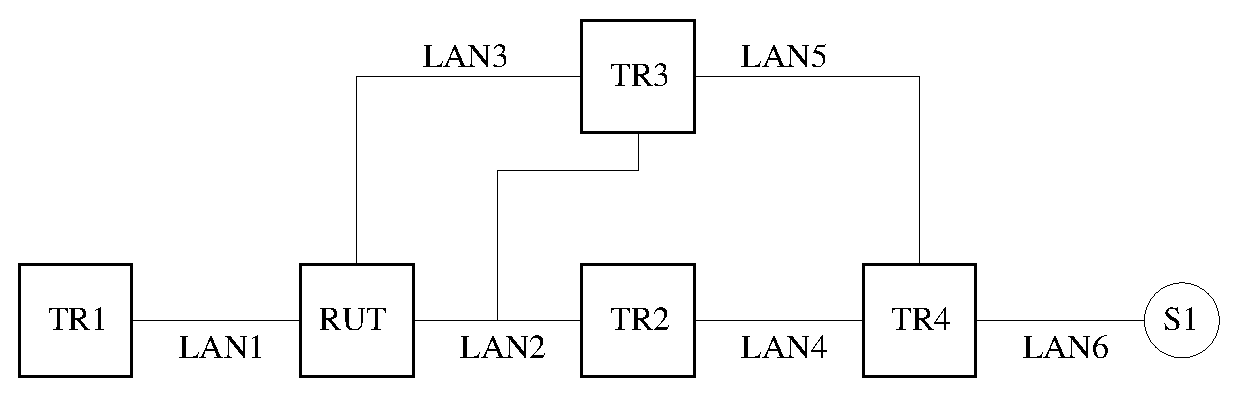
\includegraphics[scale=0.8]{figs/pim_test_4_9_state_machine_for_sg_rpt_triggered_messages}
    \caption{State machine for (S,G,rpt) triggered messages test setup}
    \label{fig:pim_test_4_9_state_machine_for_sg_rpt_triggered_messages}
  \end{center}
\end{figure}

\para{Procedure:}

\subpara{Part A: PruneDesired(S,G,rpt) $\Longrightarrow$ True transaction in
RPTNotJoined(G) state triggered by inherited\_olist(S,G,rpt) == NULL.}

\begin{enumerate}

  \item Configure the RUT such that the next hop router toward S1 is
  TR2. Start the RUT, TR1, TR2, TR3, and TR4. If necessary, wait until the
  RP-set in the RUT, TR1, TR2, TR3, and TR4 converges.

  \item Start observing the Join/Prune messages transmitted by the RUT on
  LAN2.

  \item Compose an (*,G) Join message at TR1 that contains also (S,G,rpt)
  Prune with the S address set to the address of S1, and send it to the RUT.
  The \verb=J/P_HoldTime= of the message should be set to its default
  value ({\PimsmJPHoldTime}).

  \item Observe the Join/Prune messages transmitted by the RUT on LAN2 and the
  (S,G,rpt) state in the RUT.

  \item Repeat the test with sending (*,*,RP) Join instead of (*,G) Join.

\end{enumerate}

\subpara{Part B: PruneDesired(S,G,rpt) $\Longrightarrow$ True transaction in
RPTNotJoined(G) state triggered by (SPTbit(S,G) == TRUE AND (RPF'(*,G) !=
RPF'(S,G)))}

\begin{enumerate}

  \item Configure the RUT such that the next hop router toward S1 is
  the interface that connects TR3 to LAN2. Start the RUT, TR1, TR2, TR3, and
  TR4. If necessary, wait until the RP-set in the RUT, TR1, TR2, TR3, and TR4
  converges.

  \item Start observing the Join/Prune messages transmitted by the RUT on
  LAN2.

  \item Compose an (S,G) Join message at TR1 with the S address set to the
  address of S1, and send it to the RUT. 
  The \verb=J/P_HoldTime= of the message should be set to its default
  value ({\PimsmJPHoldTime}).

  \item Start S1.

  \item Compose an (*,G) Join message at TR1, and send it to the RUT. 
  The \verb=J/P_HoldTime= of the message should be set to its default
  value ({\PimsmJPHoldTime}).

  \item Observe the Join/Prune messages transmitted by the RUT on LAN2 and the
  (S,G,rpt) state in the RUT.

  \item Repeat the test with sending (*,*,RP) Join instead of (*,G) Join.

\end{enumerate}

\subpara{Part C: PruneDesired(S,G,rpt) $\Longrightarrow$ True transaction in
NotPruned(S,G,rpt) state triggered by inherited\_olist(S,G,rpt) == NULL.}

\begin{enumerate}

  \item Configure the RUT such that the next hop router toward S1 is
  TR2. Start the RUT, TR1, TR2, TR3, and TR4. If necessary, wait until the
  RP-set in the RUT, TR1, TR2, TR3, and TR4 converges.

  \item Start observing the Join/Prune messages transmitted by the RUT on
  LAN2.

  \item Compose an (*,G) Join message at TR1, and send it to the RUT.
  The \verb=J/P_HoldTime= of the message should be set to its default
  value ({\PimsmJPHoldTime}).

  \item Compose an (S,G,rpt) Prune message at TR1 with the S address set to
  the address of S1, and send it to the RUT. The \verb=J/P_HoldTime= of the
  message should be set to its default value ({\PimsmJPHoldTime}).

  \item Observe the Join/Prune messages transmitted by the RUT on LAN2 and the
  (S,G,rpt) state in the RUT.

  \item Repeat the test with sending (*,*,RP) Join instead of (*,G) Join.

\end{enumerate}

\subpara{Part D: PruneDesired(S,G,rpt) $\Longrightarrow$ True transaction in
NotPruned(S,G,rpt) state triggered by (SPTbit(S,G) == TRUE AND (RPF'(*,G) !=
RPF'(S,G)))} 

\begin{enumerate}

  \item Configure the RUT such that the next hop router toward S1 is
  the interface that connects TR3 to LAN3. Start the RUT, TR1, TR2, TR3, and
  TR4. If necessary, wait until the RP-set in the RUT, TR1, TR2, TR3, and TR4
  converges.

  \item Start observing the Join/Prune messages transmitted by the RUT on
  LAN2.

  \item Compose an (*,G) Join message at TR1, and send it to the RUT.
  The \verb=J/P_HoldTime= of the message should be set to its default
  value ({\PimsmJPHoldTime}).

  \item Compose an (S,G) Join message at TR1 with the S address set to the
  address of S1, and send it to the RUT. 
  The \verb=J/P_HoldTime= of the message should be set to its default
  value ({\PimsmJPHoldTime}).

  \item Start S1.

  \item Observe the Join/Prune messages transmitted by the RUT on LAN2 and the
  (S,G,rpt) state in the RUT.

  \item Repeat the test with sending (*,*,RP) Join instead of (*,G) Join.

\end{enumerate}

\subpara{Part E: PruneDesired(S,G,rpt) $\Longrightarrow$ False transaction in
Pruned(S,G,rpt) state triggered by inherited\_olist(S,G,rpt) != NULL.}

\begin{enumerate}

  \item Configure the RUT such that the next hop router toward S1 is
  TR2. Start the RUT, TR1, TR2, TR3, and TR4. If necessary, wait until the
  RP-set in the RUT, TR1, TR2, TR3, and TR4 converges.

  \item Start observing the Join/Prune messages transmitted by the RUT on
  LAN2.

  \item Compose an (*,G) Join message at TR1 that contains also (S,G,rpt)
  Prune with the S address set to the address of S1, and send it to the RUT.
  The \verb=J/P_HoldTime= of the message should be set to its default
  value ({\PimsmJPHoldTime}).

  \item Observe the Join/Prune messages transmitted by the RUT on LAN2 and the
  (S,G,rpt) state in the RUT until the next periodic (*,G) Join message is
  transmitted (\ie after up to \verb=t_periodic= ({\PimsmTPeriodic})).

  \item Compose an (S,G,rpt) Join message at TR1 with the S address set to the
  address of S1, and send it to the RUT. 
  The \verb=J/P_HoldTime= of the message should be set to its default
  value ({\PimsmJPHoldTime}).

  \item Observe the Join/Prune messages transmitted by the RUT on LAN2 and the
  (S,G,rpt) state in the RUT.

  \item Repeat the test with sending (*,*,RP) Join instead of (*,G) Join.

\end{enumerate}

\subpara{Part F: PruneDesired(S,G,rpt) $\Longrightarrow$ True transaction in
Pruned(S,G,rpt) state triggered by !(SPTbit(S,G) == TRUE AND (RPF'(*,G) !=
RPF'(S,G)))}

\begin{enumerate}

  \item Configure the RUT such that the next hop router toward S1 is
  the interface that connects TR3 to LAN3. Start the RUT, TR1, TR2, TR3, and
  TR4. If necessary, wait until the RP-set in the RUT, TR1, TR2, TR3, and TR4
  converges.

  \item Start observing the Join/Prune messages transmitted by the RUT on
  LAN2.

  \item Compose an (*,G) Join message at TR1, and send it to the RUT.
  The \verb=J/P_HoldTime= of the message should be set to its default
  value ({\PimsmJPHoldTime}).

  \item Compose an (S,G) Join message at TR1 with the S address set to the
  address of S1, and send it to the RUT. 
  The \verb=J/P_HoldTime= of the message should be set to its default
  value ({\PimsmJPHoldTime}).

  \item Start S1.

  \item Observe the Join/Prune messages transmitted by the RUT on LAN2 and the
  (S,G,rpt) state in the RUT until the next periodic (*,G) Join message is
  transmitted (\ie after up to \verb=t_periodic= ({\PimsmTPeriodic})).

  \item Change the MRIB in the RUT such that the next-hop router
  router toward S1 is TR2.

  \item Observe the Join/Prune messages transmitted by the RUT on LAN2 and the
  (S,G,rpt) state in the RUT.

  \item Repeat the test with sending (*,*,RP) Join instead of (*,G) Join.

\end{enumerate}

\subpara{Part G: RPTJoinDesired(G) $\Longrightarrow$ False transaction in
Pruned(S,G,rpt) state.}

\begin{enumerate}

  \item Configure the RUT such that the next hop router toward S1 is
  TR2. Start the RUT, TR1, TR2, TR3, and TR4. If necessary, wait until the
  RP-set in the RUT, TR1, TR2, TR3, and TR4 converges.

  \item Start observing the Join/Prune messages transmitted by the RUT on
  LAN2.

  \item Compose an (*,G) Join message at TR1 that contains also (S,G,rpt)
  Prune with the S address set to the address of S1, and send it to the RUT.
  The \verb=J/P_HoldTime= of the message should be set to its default
  value ({\PimsmJPHoldTime}).

  \item Observe the Join/Prune messages transmitted by the RUT on LAN2 and the
  (S,G,rpt) state in the RUT until the next periodic (*,G) Join message is
  transmitted (\ie after up to \verb=t_periodic= ({\PimsmTPeriodic})).

  \item Compose an (*,G) Prune message at TR1, and send it to the RUT. 
  The \verb=J/P_HoldTime= of the message should be set to its default
  value ({\PimsmJPHoldTime}).

  \item Observe the Join/Prune messages transmitted by the RUT on LAN2 and the
  (S,G,rpt) state in the RUT.

  \item Repeat the test with sending (*,*,RP) Join/Prune instead of (*,G)
  Join/Prune.

\end{enumerate}

\subpara{Part H: RPTJoinDesired(G) $\Longrightarrow$ False transaction in
NotPruned(S,G,rpt) state.}

\begin{enumerate}

  \item Configure the RUT such that the next hop router toward S1 is
  TR2. Start the RUT, TR1, TR2, TR3, and TR4. If necessary, wait until the
  RP-set in the RUT, TR1, TR2, TR3, and TR4 converges.

  \item Start observing the Join/Prune messages transmitted by the RUT on
  LAN2.

  \item Compose an (*,G) Join message at TR3, and send it to the RUT on LAN3.
  The \verb=J/P_HoldTime= of the message should be set to its default
  value ({\PimsmJPHoldTime}).

  \item Compose an (*,G) Join message at TR1 that contains also (S,G,rpt)
  Prune with the S address set to the address of S1, and send it to the RUT.
  The \verb=J/P_HoldTime= of the message should be set to its default
  value ({\PimsmJPHoldTime}).

  \item Observe the Join/Prune messages transmitted by the RUT on LAN2 and the
  (S,G,rpt) state in the RUT until the next periodic (*,G) Join message is
  transmitted (\ie after up to \verb=t_periodic= ({\PimsmTPeriodic})).

  \item Compose an (*,G) Prune message at TR1, and send it to the RUT. 
  The \verb=J/P_HoldTime= of the message should be set to its default
  value ({\PimsmJPHoldTime}).

  \item Compose an (*,G) Prune message at TR3, and send it to the RUT on LAN3.
  The \verb=J/P_HoldTime= of the message should be set to its default
  value ({\PimsmJPHoldTime}).

  \item Observe the Join/Prune messages transmitted by the RUT on LAN2 and the
  (S,G,rpt) state in the RUT.

  \item Repeat the test with sending (*,*,RP) Join/Prune instead of (*,G)
  Join/Prune.

\end{enumerate}

\subpara{Part I: inherited\_olist(S,G,rpt) $\Longrightarrow$ non-NULL
transaction in RPTNotJoined(G) state.}

  The need for performing this test is implementation-specific. For example,
  it may not be possible to perform it if an implementation removes
  (S,G,rpt) entry that is in RPTNotJoined(G) state. The procedure below
  assumes that an implementation temporary keeps (S,G,rpt) entries that are in
  RPTNotJoined(G) state (\eg if the (S,G,rpt) entry is removed only after all
  downstream (S,G,rpt) state machines are in NoInfo state, or only after the
  corresponding (*,G) entry is removed as well).

\begin{enumerate}

  \item Use an implementation-specific procedure to create an (S,G,rpt) entry
  that is in RPTNotJoined(G) state, and whose all downstream state machine is
  in NoInfo state. For example, one candidate is the procedure in Part G
  (an (S,G,rpt) entry may exists at the end of the test).

  \item Observe the (S,G,rpt) state in the RUT.

  \item Compose an (*,G) Join message at TR1, and send it to the RUT.
  The \verb=J/P_HoldTime= of the message should be set to its default
  value ({\PimsmJPHoldTime}).

  \item Observe the (S,G,rpt) state in the RUT.

  \item Repeat the test with sending (*,*,RP) Join instead of (*,G)
  Join.

\end{enumerate}

\subpara{Part J: Prune override behavior in NotPruned(S,G,rpt) state.}

\begin{enumerate}

  \item Configure the RUT such that the next hop router toward S1 is
  TR2. Start the RUT, TR1, TR2, TR3, and TR4. If necessary, wait until the
  RP-set in the RUT, TR1, TR2, TR3, and TR4 converges.

  \item Start observing the Join/Prune messages transmitted by the RUT on
  LAN2.

  \item Compose an (*,G) Join message at TR3, and send it to the RUT on LAN3.
  The \verb=J/P_HoldTime= of the message should be set to its default
  value ({\PimsmJPHoldTime}).

  \item Compose an (*,G) Join message at TR1 that contains also (S,G,rpt)
  Prune with the S address set to the address of S1, and send it to the RUT.
  The \verb=J/P_HoldTime= of the message should be set to its default
  value ({\PimsmJPHoldTime}).

  \item Observe the Join/Prune messages transmitted by the RUT on LAN2 and the
  (S,G,rpt) state in the RUT.

  \item Compose an (S,G,rpt) Prune message at TR3 with the S address set to
  the address of S1, and send it on LAN2 with the upstream neighbor address
  set to TR2.
  The \verb=J/P_HoldTime= of the message should be set to its default
  value ({\PimsmJPHoldTime}).

  \item Observe the Join/Prune messages transmitted by the RUT on LAN2 and the
  (S,G,rpt) state in the RUT for at least \verb=t_override=
  ({\PimsmTOverride}).

  \item Compose an (S,G,rpt) Prune message at TR3 with the S address set to
  the address of S1, and send it on LAN2 with the upstream neighbor address
  set to TR2. Immediately after that compose an (S,G,rpt) Join message at TR3
  with the S address set to the address of S1, and send it on LAN2 with the
  upstream neighbor address set to TR2.
  The \verb=J/P_HoldTime= of both messages should be set to the default
  value ({\PimsmJPHoldTime}).

  \item Observe the Join/Prune messages transmitted by the RUT on LAN2 and the
  (S,G,rpt) state in the RUT for at least \verb=t_override=
  ({\PimsmTOverride}).

  \item Compose an (S,G) Prune message at TR3 with the S address set to
  the address of S1, and send it on LAN2 with the upstream neighbor address
  set to TR2.
  The \verb=J/P_HoldTime= of the message should be set to its default
  value ({\PimsmJPHoldTime}).

  \item Observe the Join/Prune messages transmitted by the RUT on LAN2 and the
  (S,G,rpt) state in the RUT for at least \verb=t_override=
  ({\PimsmTOverride}).

  \item Trigger changing of RPF'(S,G,rpt) at the RUT to TR3 by composing an
  (S,G) Assert message at TR3 with RPT-bit, metric and metric 
  preference set to zero, and sending it on LAN2.

  \item Keep observing the Join/Prune messages transmitted by the
  RUT on LAN2 until the next (*,G) Join message is transmitted on
  LAN2 (\ie for at least \verb=t_periodic= ({\PimsmTPeriodic})).

  \item Trigger changing of RPF'(S,G,rpt) at the RUT to TR2 by composing an
  (S,G) Assert message at TR3 with RPT-bit set to zero, metric and metric 
  preference set to 10000, and sending it on LAN2. Right after that
  compose an (S,G) Assert message at TR2 with RPT-bit, metric and metric 
  preference set to zero, and send it on LAN2.

  \item Observe the Join/Prune messages transmitted by the RUT on LAN2 and the
  (S,G,rpt) state in the RUT for at least \verb=t_override=
  ({\PimsmTOverride}).

  \item Repeat the test with sending (*,*,RP) Join instead of (*,G)
  Join.

\end{enumerate}


\para{Observable Results:}

\subpara{Part A:}

\begin{itemize}

  \item After TR1 sends the (*,G) Join and (S,G,rpt) Prune message to the RUT,
  the RUT itself should transmit an (*,G) Join and (S,G,rpt) Prune message on
  LAN2 with the upstream neighbor address set to TR2. The interface that
  connects the RUT to LAN1 should be added to the set of joined interfaces for
  the corresponding (*,G) routing state, and to the set of interfaces that are
  in Prune state for the corresponding (S,G,rpt) routing state. The (*,G)
  upstream state should be Joined; the (S,G,rpt) upstream state should be
  Pruned. The inherited\_olist(S,G,rpt) should be empty:

\begin{verbatim}
Xorp> show pim join 
Group           Source          RP              Flags
224.0.1.20      0.0.0.0         10.4.0.1        WC   
    Upstream interface (RP):   dc1
    Upstream MRIB next hop (RP): 10.2.0.2
    Upstream RPF'(*,G):        10.2.0.2
    Upstream state:            Joined 
    Join timer:                54
    Local receiver include WC: ..............
    Joins RP:                  ..............
    Joins WC:                  ........O.....
    Join state:                ........O.....
    Prune state:               ..............
    Prune pending state:       ..............
    I am assert winner state:  ..............
    I am assert loser state:   ..............
    Assert winner WC:          ..............
    Assert lost WC:            ..............
    Assert tracking WC:        .....O..O.....
    Could assert WC:           ........O.....
    I am DR:                   ........O.....
    Immediate olist RP:        ..............
    Immediate olist WC:        ........O.....
    Inherited olist SG:        ..............
    Inherited olist SG_RPT:    ..............
    PIM include WC:            ..............
224.0.1.20      10.4.0.2        10.4.0.1        SG_RPT 
    Upstream interface (S):    dc1
    Upstream interface (RP):   dc1
    Upstream MRIB next hop (RP): 10.2.0.2
    Upstream RPF'(S,G,rpt):    10.2.0.2
    Upstream state:            Pruned 
    Override timer:           -1
    Local receiver include WC: ..............
    Joins RP:                  ..............
    Joins WC:                  ........O.....
    Prunes SG_RPT:             ........O.....
    Join state:                ..............
    Prune state:               ........O.....
    Prune pending state:       ..............
    Prune tmp state:           ..............
    Prune pending tmp state:   ..............
    Assert winner WC:          ..............
    Assert lost WC:            ..............
    Assert lost SG_RPT:        ..............
    Assert tracking SG:        ..............
    Could assert WC:           ........O.....
    Could assert SG:           ..............
    I am DR:                   ........O.....
    Immediate olist RP:        ..............
    Immediate olist WC:        ........O.....
    Inherited olist SG:        ..............
    Inherited olist SG_RPT:    ..............
    PIM include WC:            ..............
\end{verbatim}

  \item When the test is repeated with sending (*,*,RP) Join instead of (*,G)
  Join, the results should be similar:

\begin{verbatim}
Xorp> show pim join 
Group           Source          RP              Flags
224.0.0.0       10.4.0.1        10.4.0.1        RP   
    Upstream interface (RP):   dc1
    Upstream MRIB next hop (RP): 10.2.0.2
    Upstream state:            Joined 
    Join timer:                49
    Joins RP:                  ........O.....
    Join state:                ........O.....
    Prune state:               ..............
    Prune pending state:       ..............
    Could assert WC:           ........O.....
    I am DR:                   ........O.....
    Immediate olist RP:        ........O.....
    Inherited olist SG:        ..............
    Inherited olist SG_RPT:    ..............
224.0.1.20      10.4.0.2        10.4.0.1        SG_RPT 
    Upstream interface (S):    dc1
    Upstream interface (RP):   dc1
    Upstream MRIB next hop (RP): 10.2.0.2
    Upstream RPF'(S,G,rpt):    10.2.0.2
    Upstream state:            Pruned 
    Override timer:           -1
    Local receiver include WC: ..............
    Joins RP:                  ........O.....
    Joins WC:                  ..............
    Prunes SG_RPT:             ........O.....
    Join state:                ..............
    Prune state:               ........O.....
    Prune pending state:       ..............
    Prune tmp state:           ..............
    Prune pending tmp state:   ..............
    Assert winner WC:          ..............
    Assert lost WC:            ..............
    Assert lost SG_RPT:        ..............
    Assert tracking SG:        ..............
    Could assert WC:           ........O.....
    Could assert SG:           ..............
    I am DR:                   ........O.....
    Immediate olist RP:        ........O.....
    Immediate olist WC:        ..............
    Inherited olist SG:        ..............
    Inherited olist SG_RPT:    ..............
    PIM include WC:            ..............
\end{verbatim}

  % TODO: XXX: after the spec if fixed, remove this?
  Note that the (*,*,RP) Join message generated by the RUT might not include
  (S,G,rpt) Prune (see the list of possible problems at the end of this
  section).

\end{itemize}

\subpara{Part B:}

\begin{itemize}

  \item After TR1 sends the (S,G) Join, the RUT should create (S,G) routing
  state, and should transmit an (S,G) Join on LAN2 with the upstream neighbor
  address set to TR3.

  \item After S1 is started, the SPT bit for the (S,G) routing state in the
  RUT should be set:
\begin{verbatim}
Xorp> show pim join 
Group           Source          RP              Flags
224.0.1.20      10.4.0.2        10.4.0.1        SG SPT 
<del>
\end{verbatim}

  \item After TR1 sends the (*,G) Join to the RUT,
  the RUT itself should transmit an (*,G) Join and (S,G,rpt) Prune message on
  LAN2 with the upstream neighbor address set to TR2. The interface that
  connects the RUT to LAN1 should be added to the set of joined interfaces for
  the corresponding (*,G) routing state. The (*,G)
  upstream state should be Joined; the (S,G,rpt) upstream state should be
  Pruned. The inherited\_olist(S,G,rpt) should not be empty:

\begin{verbatim}
Xorp> show pim join 
Group           Source          RP              Flags
224.0.1.20      0.0.0.0         10.4.0.1        WC   
    Upstream interface (RP):   dc1
    Upstream MRIB next hop (RP): 10.2.0.2
    Upstream RPF'(*,G):        10.2.0.2
    Upstream state:            Joined 
    Join timer:                53
    Local receiver include WC: ..............
    Joins RP:                  ..............
    Joins WC:                  ........O.....
    Join state:                ........O.....
    Prune state:               ..............
    Prune pending state:       ..............
    I am assert winner state:  ..............
    I am assert loser state:   ..............
    Assert winner WC:          ..............
    Assert lost WC:            ..............
    Assert tracking WC:        .....O..O.....
    Could assert WC:           ........O.....
    I am DR:                   ........O.....
    Immediate olist RP:        ..............
    Immediate olist WC:        ........O.....
    Inherited olist SG:        ..............
    Inherited olist SG_RPT:    ..............
    PIM include WC:            ..............
224.0.1.20      10.4.0.2        10.4.0.1        SG_RPT 
    Upstream interface (S):    dc1
    Upstream interface (RP):   dc1
    Upstream MRIB next hop (RP): 10.2.0.2
    Upstream RPF'(S,G,rpt):    10.2.0.2
    Upstream state:            Pruned 
    Override timer:           -1
    Local receiver include WC: ..............
    Joins RP:                  ..............
    Joins WC:                  ........O.....
    Prunes SG_RPT:             ..............
    Join state:                ..............
    Prune state:               ..............
    Prune pending state:       ..............
    Prune tmp state:           ..............
    Prune pending tmp state:   ..............
    Assert winner WC:          ..............
    Assert lost WC:            ..............
    Assert lost SG_RPT:        ..............
    Could assert WC:           ........O.....
    Could assert SG:           ........O.....
    I am DR:                   ........O.....
    Immediate olist RP:        ..............
    Immediate olist WC:        ........O.....
    Inherited olist SG:        ..............
    Inherited olist SG_RPT:    ........O.....
    PIM include WC:            ..............
224.0.1.20      10.4.0.2        10.4.0.1        SG SPT 
    Upstream interface (S):    dc1
    Upstream interface (RP):   dc1
    Upstream MRIB next hop (RP): 10.2.0.2
    Upstream MRIB next hop (S):  10.2.0.4
    Upstream RPF'(S,G):        10.2.0.4
    Upstream state:            Joined 
    Join timer:                47
    Local receiver include WC: ..............
    Local receiver include SG: ..............
    Local receiver exclude SG: ..............
    Joins RP:                  ..............
    Joins WC:                  ........O.....
    Joins SG:                  ........O.....
    Join state:                ........O.....
    Prune state:               ..............
    Prune pending state:       ..............
    I am assert winner state:  ..............
    I am assert loser state:   ..............
    Assert winner WC:          ..............
    Assert winner SG:          ..............
    Assert lost WC:            ..............
    Assert lost SG:            ..............
    Assert lost SG_RPT:        ..............
    Assert tracking SG:        .....O..O.....
    Could assert WC:           ........O.....
    Could assert SG:           ........O.....
    I am DR:                   ........O.....
    Immediate olist RP:        ..............
    Immediate olist WC:        ........O.....
    Immediate olist SG:        ........O.....
    Inherited olist SG:        ........O.....
    Inherited olist SG_RPT:    ..............
    PIM include WC:            ..............
    PIM include SG:            ..............
    PIM exclude SG:            ..............
\end{verbatim}

  After that the RUT should continue sending periodic (S,G) Join messages on
  LAN2 with the upstream neighbor address set to TR3, and periodic (*,G) Join
  with included (S,G,rpt) Prune messages on LAN2 with the upstream neighbor
  address set to TR2.

  \item When the test is repeated with sending (*,*,RP) Join instead of (*,G)
  Join, the results should be similar.

\end{itemize}

\subpara{Part C:}

\begin{itemize}

  \item After TR1 sends the (*,G) Join message to the RUT, the RUT itself
  should transmit an (*,G) Join message on LAN2 with the upstream neighbor
  address set to TR2. The interface that connects the RUT to LAN1 should be
  added to the set of joined interfaces for the corresponding (*,G) routing
  state. The (*,G) upstream state should be Joined.

  \item After TR1 sends the (S,G,rpt) Prune message to the RUT, the RUT itself
  should transmit an (S,G,rpt) Prune message on LAN2 with the upstream
  neighbor address set to TR2. The rest of the results should be same as in
  Part A.

  \item When the test is repeated with sending (*,*,RP) Join instead of (*,G)
  Join, the results should be similar.
  % TODO: XXX: after the spec if fixed, remove this?
  Note that the (*,*,RP) Join message generated by the RUT might not include
  (S,G,rpt) Prune (see the list of possible problems at the end of this
  section).

\end{itemize}

\subpara{Part D:}

\begin{itemize}

  \item After TR1 sends the (*,G) Join message to the RUT, the RUT itself
  should transmit an (*,G) Join message on LAN2 with the upstream neighbor
  address set to TR2. The interface that connects the RUT to LAN1 should be
  added to the set of joined interfaces for the corresponding (*,G) routing
  state. The (*,G) upstream state should be Joined.

  \item After TR1 sends the (S,G) Join message to the RUT, the RUT itself
  should transmit an (S,G) Join message on LAN3 with the upstream neighbor
  address set to TR3. The interface that connects the RUT to LAN1 should be
  added to the set of joined interfaces for the corresponding (S,G) routing
  state. The (S,G) upstream state should be Joined.

  \item After S1 is started, the SPT bit for the (S,G) routing state in the
  RUT should be set:
\begin{verbatim}
Xorp> show pim join 
Group           Source          RP              Flags
224.0.1.20      10.4.0.2        10.4.0.1        SG SPT 
<del>
\end{verbatim}

  Right after the SPT bit is set, the RUT should transmit (S,G,rpt) Prune
  message on LAN2 with the upstream neighbor address set to TR2 (\ie toward
  RPF'(S,G,rpt)). The (S,G,rpt) upstream state inside the RUT should be
  Pruned:

\begin{verbatim}
Xorp> show pim join 
Group           Source          RP              Flags
224.0.1.20      0.0.0.0         10.4.0.1        WC   
    Upstream interface (RP):   dc1
    Upstream MRIB next hop (RP): 10.2.0.2
    Upstream RPF'(*,G):        10.2.0.2
    Upstream state:            Joined 
    Join timer:                31
    Local receiver include WC: ..............
    Joins RP:                  ..............
    Joins WC:                  ........O.....
    Join state:                ........O.....
    Prune state:               ..............
    Prune pending state:       ..............
    I am assert winner state:  ..............
    I am assert loser state:   ..............
    Assert winner WC:          ..............
    Assert lost WC:            ..............
    Assert tracking WC:        .....O..O.....
    Could assert WC:           ........O.....
    I am DR:                   ........O.....
    Immediate olist RP:        ..............
    Immediate olist WC:        ........O.....
    Inherited olist SG:        ..............
    Inherited olist SG_RPT:    ..............
    PIM include WC:            ..............
224.0.1.20      10.4.0.2        10.4.0.1        SG_RPT 
    Upstream interface (S):    dc2
    Upstream interface (RP):   dc1
    Upstream MRIB next hop (RP): 10.2.0.2
    Upstream RPF'(S,G,rpt):    10.2.0.2
    Upstream state:            Pruned 
    Override timer:           -1
    Local receiver include WC: ..............
    Joins RP:                  ..............
    Joins WC:                  ........O.....
    Prunes SG_RPT:             ..............
    Join state:                ..............
    Prune state:               ..............
    Prune pending state:       ..............
    Prune tmp state:           ..............
    Prune pending tmp state:   ..............
    Assert winner WC:          ..............
    Assert lost WC:            ..............
    Assert lost SG_RPT:        ..............
    Could assert WC:           ........O.....
    Could assert SG:           ........O.....
    I am DR:                   ........O.....
    Immediate olist RP:        ..............
    Immediate olist WC:        ........O.....
    Inherited olist SG:        ..............
    Inherited olist SG_RPT:    ........O.....
    PIM include WC:            ..............
224.0.1.20      10.4.0.2        10.4.0.1        SG SPT 
    Upstream interface (S):    dc2
    Upstream interface (RP):   dc1
    Upstream MRIB next hop (RP): 10.2.0.2
    Upstream MRIB next hop (S):  10.8.0.2
    Upstream RPF'(S,G):        10.8.0.2
    Upstream state:            Joined 
    Join timer:                36
    Local receiver include WC: ..............
    Local receiver include SG: ..............
    Local receiver exclude SG: ..............
    Joins RP:                  ..............
    Joins WC:                  ........O.....
    Joins SG:                  ........O.....
    Join state:                ........O.....
    Prune state:               ..............
    Prune pending state:       ..............
    I am assert winner state:  ..............
    I am assert loser state:   ..............
    Assert winner WC:          ..............
    Assert winner SG:          ..............
    Assert lost WC:            ..............
    Assert lost SG:            ..............
    Assert lost SG_RPT:        ..............
    Assert tracking SG:        ......O.O.....
    Could assert WC:           ........O.....
    Could assert SG:           ........O.....
    I am DR:                   ........O.....
    Immediate olist RP:        ..............
    Immediate olist WC:        ........O.....
    Immediate olist SG:        ........O.....
    Inherited olist SG:        ........O.....
    Inherited olist SG_RPT:    ..............
    PIM include WC:            ..............
    PIM include SG:            ..............
    PIM exclude SG:            ..............
\end{verbatim}

  After that the RUT should continue sending periodic (*,G) Join
  with included (S,G,rpt) Prune messages on LAN2 with the upstream neighbor
  address set to TR2, and periodic (S,G) Join on LAN3 with the upstream
  neighbor address set to TR3.

  \item When the test is repeated with sending (*,*,RP) Join instead of (*,G)
  Join, the results should be similar.
  % TODO: XXX: after the spec if fixed, remove this?
  Note that the (*,*,RP) Join message generated by the RUT might not include
  (S,G,rpt) Prune (see the list of possible problems at the end of this
  section).

\end{itemize}

\subpara{Part E:}

\begin{itemize}

  \item Until before TR1 sends the (S,G,rpt) Join message to the RUT, the
  results should be same as in Part A.

  \item After the (S,G,rpt) Join message is transmitted, the RUT itself should
  transmit an (S,G,rpt) Join message on LAN2 with the upstream neighbor
  address set to TR2. The interface that connects the RUT to LAN1 should be
  removed from the set of interfaces that are in Pruned state, and the
  (S,G,rpt) upstream state should be Not Pruned (or the (S,G,rpt) entry itself
  might be removed).

  \item When the test is repeated with sending (*,*,RP) Join instead of (*,G)
  Join, the results should be similar.
  % TODO: XXX: after the spec if fixed, remove this?
  Note that the (*,*,RP) Join message generated by the RUT might not include
  (S,G,rpt) Prune (see the list of possible problems at the end of this
  section).

\end{itemize}

\subpara{Part F:}

\begin{itemize}

  \item Until before the MRIB in the RUT is changed, the results should be
  same as in Part D. 

  \item After the MRIB in the RUT is changed, the RUT itself
  should transmit an (S,G,rpt) Join message on LAN2 with the upstream neighbor
  address set to TR2 (note that the (S,G) state machine will trigger (S,G)
  Join generation toward TR2, therefore the (S,G) Join and (S,G,rpt) Join
  might be in the same message). The (S,G,rpt) upstream state should be Not
  Pruned (or the (S,G,rpt) entry itself might be removed).

  \item When the test is repeated with sending (*,*,RP) Join instead of (*,G)
  Join, the results should be similar.
  % TODO: XXX: after the spec if fixed, remove this?
  Note that the (*,*,RP) Join message generated by the RUT might not include
  (S,G,rpt) Prune (see the list of possible problems at the end of this
  section).

\end{itemize}

\subpara{Part G:}

\begin{itemize}

  \item Until before TR1 sends the (*,G) Prune message to the RUT, the
  results should be same as in Part E.

  \item After the (*,G) Prune message is transmitted, the RUT itself should
  transmit an (*,G) Prune message on LAN2 with the upstream neighbor
  address set to TR2. The interface that connects the RUT to LAN1 should be
  removed from the set of interfaces that are in (*,G) Join state. The
  (S,G,rpt) upstream state should be RPTNotJoined(G) (or the (S,G,rpt) entry
  itself might be removed).

  \item When the test is repeated with sending (*,*,RP) Join instead of (*,G)
  Join, the results should be similar.
  % TODO: XXX: after the spec if fixed, remove this?
  Note that the (*,*,RP) Join message generated by the RUT might not include
  (S,G,rpt) Prune (see the list of possible problems at the end of this
  section).

\end{itemize}

\subpara{Part H:}

\begin{itemize}

  \item After both TR3 and TR1 have transmitted their first messages to the
  RUT, the RUT should contain (*,G) entry that is in Joined state, and
  (S,G,rpt) entry that is in NotPruned state:

\begin{verbatim}
Xorp> show pim join 
Group           Source          RP              Flags
224.0.1.20      0.0.0.0         10.4.0.1        WC   
    Upstream interface (RP):   dc1
    Upstream MRIB next hop (RP): 10.2.0.2
    Upstream RPF'(*,G):        10.2.0.2
    Upstream state:            Joined 
    Join timer:                32
    Local receiver include WC: ..............
    Joins RP:                  ..............
    Joins WC:                  ......O.O.....
    Join state:                ......O.O.....
    Prune state:               ..............
    Prune pending state:       ..............
    I am assert winner state:  ..............
    I am assert loser state:   ..............
    Assert winner WC:          ..............
    Assert lost WC:            ..............
    Assert tracking WC:        .....OO.O.....
    Could assert WC:           ......O.O.....
    I am DR:                   ........O.....
    Immediate olist RP:        ..............
    Immediate olist WC:        ......O.O.....
    Inherited olist SG:        ..............
    Inherited olist SG_RPT:    ..............
    PIM include WC:            ..............
224.0.1.20      10.4.0.2        10.4.0.1        SG_RPT 
    Upstream interface (S):    dc1
    Upstream interface (RP):   dc1
    Upstream MRIB next hop (RP): 10.2.0.2
    Upstream RPF'(S,G,rpt):    10.2.0.2
    Upstream state:            NotPruned 
    Override timer:           -1
    Local receiver include WC: ..............
    Joins RP:                  ..............
    Joins WC:                  ......O.O.....
    Prunes SG_RPT:             ........O.....
    Join state:                ..............
    Prune state:               ........O.....
    Prune pending state:       ..............
    Prune tmp state:           ..............
    Prune pending tmp state:   ..............
    Assert winner WC:          ..............
    Assert lost WC:            ..............
    Assert lost SG_RPT:        ..............
    Could assert WC:           ......O.O.....
    Could assert SG:           ..............
    I am DR:                   ........O.....
    Immediate olist RP:        ..............
    Immediate olist WC:        ......O.O.....
    Inherited olist SG:        ..............
    Inherited olist SG_RPT:    ......O.......
    PIM include WC:            ..............
\end{verbatim}

  \item After TR1 transmits the (*,G) Prune message to the RUT, the (*,G) and
  (S,G,rpt) entries in the RUT should still be respectively in Joined state
  and NotPruned state:

\begin{verbatim}
Xorp> show pim join 
Group           Source          RP              Flags
224.0.1.20      0.0.0.0         10.4.0.1        WC   
    Upstream interface (RP):   dc1
    Upstream MRIB next hop (RP): 10.2.0.2
    Upstream RPF'(*,G):        10.2.0.2
    Upstream state:            Joined 
    Join timer:                34
    Local receiver include WC: ..............
    Joins RP:                  ..............
    Joins WC:                  ......O.......
    Join state:                ......O.......
    Prune state:               ..............
    Prune pending state:       ..............
    I am assert winner state:  ..............
    I am assert loser state:   ..............
    Assert winner WC:          ..............
    Assert lost WC:            ..............
    Assert tracking WC:        .....OO.......
    Could assert WC:           ......O.......
    I am DR:                   ........O.....
    Immediate olist RP:        ..............
    Immediate olist WC:        ......O.......
    Inherited olist SG:        ..............
    Inherited olist SG_RPT:    ..............
    PIM include WC:            ..............
224.0.1.20      10.4.0.2        10.4.0.1        SG_RPT 
    Upstream interface (S):    dc1
    Upstream interface (RP):   dc1
    Upstream MRIB next hop (RP): 10.2.0.2
    Upstream RPF'(S,G,rpt):    10.2.0.2
    Upstream state:            NotPruned 
    Override timer:           -1
    Local receiver include WC: ..............
    Joins RP:                  ..............
    Joins WC:                  ......O.......
    Prunes SG_RPT:             ........O.....
    Join state:                ..............
    Prune state:               ........O.....
    Prune pending state:       ..............
    Prune tmp state:           ..............
    Prune pending tmp state:   ..............
    Assert winner WC:          ..............
    Assert lost WC:            ..............
    Assert lost SG_RPT:        ..............
    Could assert WC:           ......O.......
    Could assert SG:           ..............
    I am DR:                   ........O.....
    Immediate olist RP:        ..............
    Immediate olist WC:        ......O.......
    Inherited olist SG:        ..............
    Inherited olist SG_RPT:    ......O.......
    PIM include WC:            ..............
\end{verbatim}

  \item After TR3 transmits the (*,G) Prune message, the RUT
  itself should transmit an (*,G) Prune message on LAN2 with the upstream
  neighbor address set to TR2, and the (*,G) entry inside the RUT should be
  removed. The (S,G,rpt) upstream state should be RPTNotJoined(G) (or the
  (S,G,rpt) entry itself might be removed):

\begin{verbatim}
Xorp> show pim join 
Group           Source          RP              Flags
224.0.1.20      10.4.0.2        10.4.0.1        SG_RPT 
    Upstream interface (S):    dc1
    Upstream interface (RP):   dc1
    Upstream MRIB next hop (RP): 10.2.0.2
    Upstream RPF'(S,G,rpt):    10.2.0.2
    Upstream state:            RPTNotJoined 
    Override timer:           -1
    Local receiver include WC: ..............
    Joins RP:                  ..............
    Joins WC:                  ..............
    Prunes SG_RPT:             ........O.....
    Join state:                ..............
    Prune state:               ........O.....
    Prune pending state:       ..............
    Prune tmp state:           ..............
    Prune pending tmp state:   ..............
    Assert winner WC:          ..............
    Assert lost WC:            ..............
    Assert lost SG_RPT:        ..............
    Could assert WC:           ..............
    Could assert SG:           ..............
    I am DR:                   ........O.....
    Immediate olist RP:        ..............
    Immediate olist WC:        ..............
    Inherited olist SG:        ..............
    Inherited olist SG_RPT:    ..............
    PIM include WC:            ..............
\end{verbatim}

  \item When the test is repeated with sending (*,*,RP) Join instead of (*,G)
  Join, the results should be similar.
  % TODO: XXX: after the spec if fixed, remove this?
  Note that the (*,*,RP) Join message generated by the RUT might not include
  (S,G,rpt) Prune (see the list of possible problems at the end of this
  section).

\end{itemize}

\subpara{Part I:}

\begin{itemize}

  \item After the (*,G) Join message is transmitted, the (S,G,rpt) upstream
  state should be NotPruned.

  \item When the test is repeated with sending (*,*,RP) Join instead of (*,G)
  Join, the results should be similar.

\end{itemize}

\subpara{Part J:}

\begin{itemize}

  \item Until before TR3 transmits the (S,G,rpt) Prune message, the results
  should be same as in Part H. In other words, the RUT should have an (*,G)
  entry and an (S,G,rpt) entry that are respectively in Joined state and
  NotPruned state.

  \item After TR3 transmits its first (S,G,rpt) Prune message, the Override
  Timer of the (S,G,rpt) entry in the RUT should be set to the short random
  value of \verb=t_override= ({\PimsmTOverride}).

  \item After the Override Timer of the (S,G,rpt) entry in the RUT expires,
  the RUT should transmit an (S,G,rpt) Join on LAN2 with the upstream neighbor
  address set to TR2.

  \item After TR3 transmits its second (S,G,rpt) Prune message on LAN2
  immediately followed by an (S,G,rpt) Join, the Override Timer of the
  (S,G,rpt) entry in the RUT that was set to \verb=t_override=
  ({\PimsmTOverride}) by the (S,G,rpt) Prune message should be canceled by the
  (S,G,rpt) Join message. As a result, the RUT should not transmit (S,G,rpt)
  Join message within the short random interval of \verb=t_override=
  ({\PimsmTOverride}).

  \item After TR3 transmits the (S,G) Prune message, the Override
  Timer of the (S,G,rpt) entry in the RUT should be set to the short random
  value of \verb=t_override= ({\PimsmTOverride}).

  \item After the Override Timer of the (S,G,rpt) entry in the RUT expires,
  the RUT should transmit an (S,G,rpt) Join on LAN2 with the upstream neighbor
  address set to TR2.

  \item After the RPF'(S,G,rpt) at the RUT is changed to TR3 and then back to
  TR2, the Override Timer of the (S,G,rpt) entry in the RUT should be set to
  the short random value of \verb=t_override= ({\PimsmTOverride}).

  \item After the Override Timer of the (S,G,rpt) entry in the RUT expires,
  the RUT should transmit an (S,G,rpt) Join on LAN2 with the upstream neighbor
  address set to TR2.

  \item During the whole test, the (S,G,rpt) upstream state should always be
  in NotPruned state, except that while the RPF'(S,G,rpt) has changed to TR3,
  the upstream state should be in Pruned state.

  \item When the test is repeated with sending (*,*,RP) Join instead of (*,G)
  Join, the results should be similar.
  % TODO: XXX: after the spec if fixed, remove this?
  Note that the (*,*,RP) Join message generated by the RUT might not include
  (S,G,rpt) Prune (see the list of possible problems at the end of this
  section).

\end{itemize}

\para{Possible Problems:}
% TODO: XXX: PAVPAV: after the spec if fixed, remove this?
The current protocol specification (draft-ietf-pim-sm-v2-new-05.{txt,ps}) is
incomplete in 
specifying whether (*,*,RP) Join messages should include (S,G,rpt) Prune
messages, therefore the (*,*,RP) Join messages generated by the RUT may not
contain (S,G,rpt) Prune.
In Part J, if the first Assert generated by TR3 is not preferred when compared
to the assert metric of TR2, the RPF'(S,G,rpt) in the RUT will not be changed.
In Part J, after the RPF'(S,G,rpt) in the RUT is changed back to TR2, the RUT
may transmit two identical (S,G,rpt) Join messages on LAN2 with the upstream
neighbor address set to TR2 within the very short random interval
\verb=t_override= ({\PimsmTOverride}). The first one might be transmitted
immediately after the RPF'(S,G,rpt) in the RUT is changed back to TR2 (the
first (S,G,rpt) Join is triggered by the transition when PruneDesired(S,G,rpt)
becomes false, while the second (S,G,rpt) Join is triggered when the Override
Timer expires).

%%%%%%%%%%%%%%%%%%%%%%%%%%%%%%%%%%%%%%%%%%%


%%%%%%%%%%%%%%%%%%%%%%%%%%%%%%%%%%%%%%%%%%%%%%%%%%%%%%%%%%%%%%%%%%%%%%%
\chapter{PIM Assert Messages}

\para{Scope:}
Test sending and receiving of PIM Assert messages.

\para{Overview:}
Whenever on a shared LAN there is more than one upstream router that has valid
forwarding state for a packet, this may lead to packet duplication.
PIM does not attempt to prevent this from occurring. Instead, it detects when
this has happened, and uses PIM Assert messages to elect a single forwarder
amongst the upstream routers. Assert messages are also received by downstream
routers on the LAN; as a result, subsequent Join/Prune messages are sent to
the upstream router that is the Assert winner.

The granularity of the PIM Assert messages is per (S,G) or per (*,G).
In other words, the Assert winners are elected per (S,G) or per (*,G).


%%%%%%%%%%%%%%%%%%%%%%%%%%%%%%%%%%%%%%%%%%%
\newpage
\section{(S,G) Assert Message State Machine}

\para{Purpose:}
Verify that the (S,G) Assert state machine operates properly.

\para{References:}
\begin{itemize}
  \item draft-ietf-pim-sm-v2-new-05 -- Section 4.6.1
\end{itemize}

\para{Discussion:}
When a PIM-SM router receives a PIM Assert message, the per-interface
(S,G) state machine should be updated appropriately. Typically, if an
Assert message is received on an outgoing interface for the corresponding
(S,G) routing state, the router may either send Assert message on the
same interface if it considers itself as the Assert winner; if the router
considers itself as the Assert loser, it would remove that interface from the
set of outgoing interfaces. Similarly, if data packet is received on an
outgoing interface for corresponding (S,G) routing state, the router will
originate Assert message on that interface. Eventually, this Assert message
will be received by the other upstream router that has forwarded that data
packet on that LAN, and will trigger the Assert mechanism to elect the (S,G)
upstream forwarder for that LAN.

\para{Test Setup:}
Connect the RUT, TR1, TR2, TR3, TR4, and S1 according to
Figure~\ref{fig:pim_test_5_1_sg_assert_message_state_machine}.
Configure the IP address of the interface that connects TR4 to LAN6 as the RP.
Configure the RUT such that the next-hop router toward the RP is TR2.
Configure TR3 such that the next-hop router toward S1 is TR4.
Configure the RUT such that MRIB.pref(S) = 100, and MRIB.metric(S) = 100.

\begin{figure}[htbp]
  \begin{center}
    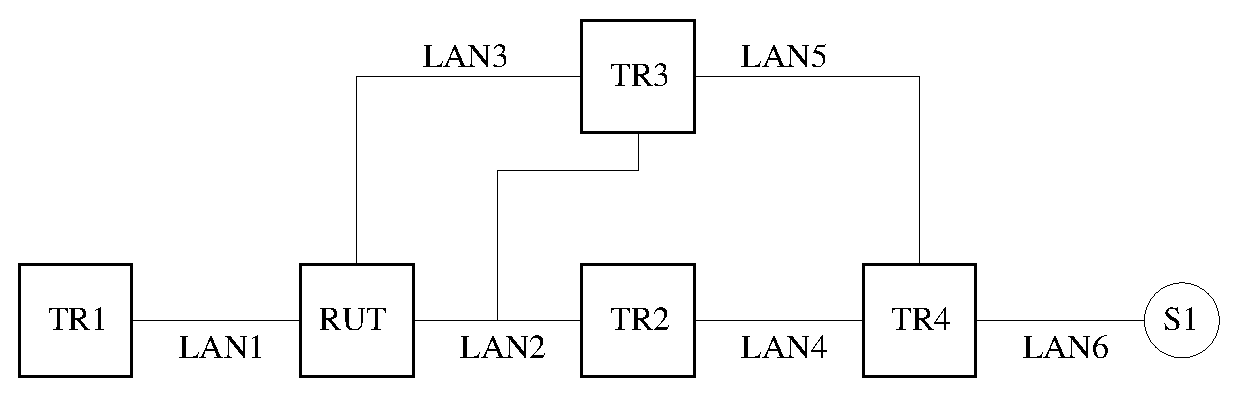
\includegraphics[scale=0.8]{figs/pim_test_5_1_sg_assert_message_state_machine}
    \caption{(S,G) Assert message state machine test setup}
    \label{fig:pim_test_5_1_sg_assert_message_state_machine}
  \end{center}
\end{figure}

\para{Procedure:}

\subpara{Part A: Receive Inferior Assert with RPTbit clear and
CouldAssert(S,G,I) in NoInfo state.}

\begin{enumerate}

  \item Start the RUT, TR1, TR2, and TR4. If necessary, wait until the RP-set
  in the RUT, TR1, TR2 and TR4 converges.

  \item Compose an (S,G) Join message at TR1 with the S address set to the
  address of S1, and send it to the RUT.
  The \verb=J/P_HoldTime= of the message should be set to its default
  value ({\PimsmJPHoldTime}).

  \item Start S1.

  \item Start observing the Assert messages transmitted by the RUT on
  LAN3, and the (S,G) Assert state in the RUT.

  \item Compose an Assert message at TR3 with the S address set to the
  address of S1, the RPT-bit set to zero, metric and metric preference set to
  1000, and send it on LAN3.

  \item Start observing the Assert messages transmitted by the RUT on
  LAN1, the (S,G) Assert state in the RUT, and the data packets forwarded on
  LAN1. 

  \item Compose an Assert message at TR1 with the S address set to the
  address of S1, the RPT-bit set to zero, metric and metric preference set to
  1000, and send it on LAN1.

  \item Continue observing the Assert messages transmitted by the RUT on
  LAN1, the (S,G) Assert state in the RUT, and the data packets forwarded on
  LAN1.

\end{enumerate}

\subpara{Part B: Receive Assert with RPTbit set and
CouldAssert(S,G,I) in NoInfo state.}

The setup is same as in Part A, except that the Assert messages that TR3 and
TR1 transmit on LAN3 and LAN1 respectively should have the RPT-bit set to one.

\subpara{Part C: Data arrives from S to G on I and
CouldAssert(S,G,I) in NoInfo state.}

\begin{enumerate}

  \item Start the RUT, TR1, TR2, and TR4. If necessary, wait until the RP-set
  in the RUT, TR1, TR2 and TR4 converges.

  \item Compose an (S,G) Join message at TR1 with the S address set to the
  address of S1, and send it to the RUT.
  The \verb=J/P_HoldTime= of the message should be set to its default
  value ({\PimsmJPHoldTime}).

  \item Start S1.

  \item Start observing the Assert messages transmitted by the RUT on
  LAN1, the (S,G) Assert state in the RUT, and the data packets forwarded on
  LAN1. 

  \item Compose a data packet at TR3 with the S address set to the
  address of S1, and send it on LAN3.

  \item Continue observing the Assert messages transmitted by the RUT on
  LAN1, the (S,G) Assert state in the RUT, and the data packets forwarded on
  LAN1.

  \item Compose a data packet at TR1 with the S address set to the
  address of S1, and send it on LAN1.

  \item Continue observing the Assert messages transmitted by the RUT on
  LAN1, the (S,G) Assert state in the RUT, and the data packets forwarded on
  LAN1.

\end{enumerate}

\subpara{Part D: Receive Preferred Assert with RPTbit clear and
AssertTrackingDesired(S,G,I) in NoInfo state.}

\begin{enumerate}

  \item Start the RUT, TR1, TR2, and TR4. If necessary, wait until the RP-set
  in the RUT, TR1, TR2 and TR4 converges.

  \item Compose an (S,G) Join message at TR1 with the S address set to the
  address of S1, and send it to the RUT.
  The \verb=J/P_HoldTime= of the message should be set to its default
  value ({\PimsmJPHoldTime}).

  \item Start observing the (S,G) Assert state in the RUT.

  \item Compose an Assert message at TR3 with the S address set to the
  address of S1, the RPT-bit set to zero, metric and metric preference set to
  10, and send it on LAN3.

  \item Continue observing the (S,G) Assert state in the RUT.

  \item Compose an Assert message at TR1 with the S address set to the
  address of S1, the RPT-bit set to zero, metric and metric preference set to
  10, and send it on LAN1.

  \item Continue observing the (S,G) Assert state in the RUT.

  \item Compose an Assert message at TR3 with the S address set to the
  address of S1, the RPT-bit set to zero, metric and metric preference set to
  10, and send it on LAN2.

  \item Continue observing the (S,G) Assert state in the RUT.

  \item Compose an (S,G) Join message at TR3 with the S address set to the
  address of S1, and send it to the RUT on LAN3.
  The \verb=J/P_HoldTime= of the message should be set to its default
  value ({\PimsmJPHoldTime}).

  \item Compose an Assert message at TR3 with the S address set to the
  address of S1, the RPT-bit set to zero, metric and metric preference set to
  10, and send it on LAN2.

  \item Continue observing the (S,G) Assert state in the RUT.

\end{enumerate}

\subpara{Part E: Timer expires in I Am Assert Winner state.}

\begin{enumerate}

  \item Start the RUT, TR1, TR2, and TR4. If necessary, wait until the RP-set
  in the RUT, TR1, TR2 and TR4 converges.

  \item Compose an (S,G) Join message at TR1 with the S address set to the
  address of S1, and send it to the RUT.
  The \verb=J/P_HoldTime= of the message should be set to its default
  value ({\PimsmJPHoldTime}).

  \item Start S1.

  \item Start observing the Assert messages transmitted by the RUT on
  LAN1, the (S,G) Assert state in the RUT, and the data packets forwarded on
  LAN1.

  \item Compose an Assert message at TR1 with the S address set to the
  address of S1, the RPT-bit set to zero, metric and metric preference set to
  1000, and send it on LAN1.

  \item Continue observing the Assert messages transmitted by the RUT on
  LAN1, the (S,G) Assert state in the RUT, and the data packets forwarded on
  LAN1 for at least \newline
  (\verb=Assert_Time= - \verb=Assert_Override_Interval=)
  ({\PimsmAssertTime} - {\PimsmAssertOverrideInterval}).
  In the mean time, every \verb=t_periodic= ({\PimsmTPeriodic}) compose same
  (S,G) Join message at TR1, and send it to the RUT.

\end{enumerate}

\subpara{Part F: Receive inferior Assert in I Am Assert Winner state.}

The setup is same as in Part A, except that TR3 does not need to transmit an
Assert message, and that TR1 transmits another Assert
message on LAN1 few seconds after its first Assert message.

\subpara{Part G: Receive Preferred Assert in I Am Assert Winner State.}

\begin{enumerate}

  \item Start the RUT, TR1, TR2, and TR4. If necessary, wait until the RP-set
  in the RUT, TR1, TR2 and TR4 converges.

  \item Compose an (S,G) Join message at TR1 with the S address set to the
  address of S1, and send it to the RUT.
  The \verb=J/P_HoldTime= of the message should be set to its default
  value ({\PimsmJPHoldTime}).

  \item Start S1.

  \item Start observing the Assert messages transmitted by the RUT on
  LAN1, the (S,G) Assert state in the RUT, and the data packets forwarded on
  LAN1. 

  \item Compose an Assert message at TR1 with the S address set to the
  address of S1, the RPT-bit set to zero, metric and metric preference set to
  1000, and send it on LAN1.

  \item Continue observing the Assert messages transmitted by the RUT on
  LAN1, the (S,G) Assert state in the RUT, and the data packets forwarded on
  LAN1.

  \item Compose an Assert message at TR1 with the S address set to the
  address of S1, the RPT-bit set to zero, metric and metric preference set to
  10, and send it on LAN1.

  \item Continue observing the Assert messages transmitted by the RUT on
  LAN1, the (S,G) Assert state in the RUT, and the data packets forwarded on
  LAN1.

\end{enumerate}

\subpara{Part H: CouldAssert(S,G,I) $\Longrightarrow$ FALSE transaction
in I Am Assert Winner state.}

\begin{enumerate}

  \item Start the RUT, TR1, TR2, and TR4. If necessary, wait until the RP-set
  in the RUT, TR1, TR2 and TR4 converges.

  \item Compose an (S,G) Join message at TR1 with the S address set to the
  address of S1, and send it to the RUT.
  The \verb=J/P_HoldTime= of the message should be set to its default
  value ({\PimsmJPHoldTime}).

  \item Compose an (S,G) Join message at TR3 with the S address set to the
  address of S1, and send it to the RUT on LAN3.
  The \verb=J/P_HoldTime= of the message should be set to its default
  value ({\PimsmJPHoldTime}).

  \item Start S1.

  \item Start observing the Assert messages transmitted by the RUT on
  LAN1, the (S,G) Assert state in the RUT, and the data packets forwarded on
  LAN1. 

  \item Compose an Assert message at TR1 with the S address set to the
  address of S1, the RPT-bit set to zero, metric and metric preference set to
  1000, and send it on LAN1.

  \item Continue observing the Assert messages transmitted by the RUT on
  LAN1, the (S,G) Assert state in the RUT, and the data packets forwarded on
  LAN1.

  \item Compose an (S,G) Prune message at TR1 with the S address set to the
  address of S1, and send it to the RUT.
  The \verb=J/P_HoldTime= of the message should be set to its default
  value ({\PimsmJPHoldTime}).

  \item Continue observing the Assert messages transmitted by the RUT on
  LAN1, the (S,G) Assert state in the RUT, and the data packets forwarded on
  LAN1.

\end{enumerate}

\subpara{Part I: Receive Preferred Assert in I Am Assert Loser State.}

\begin{enumerate}

  \item Start the RUT, TR1, TR2, and TR4. If necessary, wait until the RP-set
  in the RUT, TR1, TR2 and TR4 converges.

  \item Compose an (S,G) Join message at TR1 with the S address set to the
  address of S1, and send it to the RUT.
  The \verb=J/P_HoldTime= of the message should be set to its default
  value ({\PimsmJPHoldTime}).

  \item Start S1.

  \item Start observing the Assert messages transmitted by the RUT on
  LAN1, the (S,G) Assert state in the RUT, and the data packets forwarded on
  LAN1.

  \item Compose an Assert message at TR1 with the S address set to the
  address of S1, the RPT-bit set to zero, metric and metric preference set to
  10, and send it on LAN1.

  \item Continue observing the Assert messages transmitted by the RUT on
  LAN1, the (S,G) Assert state in the RUT, and the data packets forwarded on
  LAN1.

  \item Compose an Assert message at TR1 with the S address set to the
  address of S1, the RPT-bit set to zero, metric and metric preference set to
  1, and send it on LAN1.

  \item Continue observing the Assert messages transmitted by the RUT on
  LAN1, the (S,G) Assert state in the RUT, and the data packets forwarded on
  LAN1.

\end{enumerate}

\subpara{Part J: Receive Acceptable Assert from Current Winner in I Am Assert
Loser State.}

The setup is same as in Part I, except that the second Assert message that TR1
transmits on LAN1 should have metric and metric preference set to 50.

\subpara{Part K: Receive Inferior Assert from Current Winner in I Am Assert
Loser State.}

The setup is same as in Part I, except that the second Assert message that TR1
transmits on LAN1 should have metric and metric preference set to 1000.

\subpara{Part L: Timer expires in I Am Assert Loser State.}

\begin{enumerate}

  \item Start the RUT, TR1, TR2, and TR4. If necessary, wait until the RP-set
  in the RUT, TR1, TR2 and TR4 converges.

  \item Compose an (S,G) Join message at TR1 with the S address set to the
  address of S1, and send it to the RUT.
  The \verb=J/P_HoldTime= of the message should be set to its default
  value ({\PimsmJPHoldTime}).

  \item Start S1.

  \item Start observing the Assert messages transmitted by the RUT on
  LAN1, the (S,G) Assert state in the RUT, and the data packets forwarded on
  LAN1.

  \item Compose an Assert message at TR1 with the S address set to the
  address of S1, the RPT-bit set to zero, metric and metric preference set to
  10, and send it on LAN1.

  \item Continue observing the Assert messages transmitted by the RUT on
  LAN1, the (S,G) Assert state in the RUT, and the data packets forwarded on
  LAN1 for at least (\verb=Assert_Time=) ({\PimsmAssertTime}).

\end{enumerate}

\subpara{Part M: Current winner's GenID changes in I Am Assert Loser State.}

\begin{enumerate}

  \item Start the RUT, TR1, TR2, and TR4. If necessary, wait until the RP-set
  in the RUT, TR1, TR2 and TR4 converges.

  \item Compose an (S,G) Join message at TR1 with the S address set to the
  address of S1, and send it to the RUT.
  The \verb=J/P_HoldTime= of the message should be set to its default
  value ({\PimsmJPHoldTime}).

  \item Start S1.

  \item Start observing the Assert messages transmitted by the RUT on
  LAN1, the (S,G) Assert state in the RUT, and the data packets forwarded on
  LAN1.

  \item Compose an Assert message at TR1 with the S address set to the
  address of S1, the RPT-bit set to zero, metric and metric preference set to
  10, and send it on LAN1.

  \item Continue observing the Assert messages transmitted by the RUT on
  LAN1, the (S,G) Assert state in the RUT, and the data packets forwarded on
  LAN1.

  \item Quit TR1 (\ie stop it without graceful shutdown), and start it
  immediately.

  \item Continue observing the Assert messages transmitted by the RUT on
  LAN1, the (S,G) Assert state in the RUT, and the data packets forwarded on
  LAN1.

\end{enumerate}

\subpara{Part N: AssertTrackingDesired(S,G,I)  $\Longrightarrow$ FALSE
transaction in I Am Assert Loser State.}

\begin{enumerate}

  \item Start the RUT, TR1, TR2, and TR4. If necessary, wait until the RP-set
  in the RUT, TR1, TR2 and TR4 converges.

  \item Compose an (S,G) Join message at TR1 with the S address set to the
  address of S1, and send it to the RUT.
  The \verb=J/P_HoldTime= of the message should be set to its default
  value ({\PimsmJPHoldTime}).

  \item Start S1.

  \item Start observing the Assert messages transmitted by the RUT on
  LAN1 and LAN2, the (S,G) Assert state in the RUT, and the data packets
  forwarded on LAN1.

  \item Compose an Assert message at TR3 with the S address set to the
  address of S1, the RPT-bit set to zero, metric and metric preference set to
  10, and send it on LAN2.

  \item Continue observing the Assert messages transmitted by the RUT on
  LAN1 and LAN2, the (S,G) Assert state in the RUT, and the data packets
  forwarded on LAN1.

  \item Compose an Assert message at TR1 with the S address set to the
  address of S1, the RPT-bit set to zero, metric and metric preference set to
  10, and send it on LAN1.

  \item Continue observing the Assert messages transmitted by the RUT on
  LAN1 and LAN2, the (S,G) Assert state in the RUT, and the data packets
  forwarded on LAN1.

  \item Compose an (S,G) Join message at TR3 with the S address set to the
  address of S1, and send it to the RUT on LAN2.
  The \verb=J/P_HoldTime= of the message should be set to its default
  value ({\PimsmJPHoldTime}).

  \item Compose an (S,G) Prune message at TR1 with the S address set to the
  address of S1, and send it to the RUT.
  The \verb=J/P_HoldTime= of the message should be set to its default
  value ({\PimsmJPHoldTime}).

  \item Continue observing the Assert messages transmitted by the RUT on
  LAN1 and LAN2, the (S,G) Assert state in the RUT, and the data packets
  forwarded on LAN1.

\end{enumerate}

\subpara{Part O: my\_assert\_metric $\Longrightarrow$ better than winner's
metric in I Am Assert Loser State.}

\begin{enumerate}

  \item Start the RUT, TR1, TR2, and TR4. If necessary, wait until the RP-set
  in the RUT, TR1, TR2 and TR4 converges.

  \item Compose an (S,G) Join message at TR1 with the S address set to the
  address of S1, and send it to the RUT.
  The \verb=J/P_HoldTime= of the message should be set to its default
  value ({\PimsmJPHoldTime}).

  \item Compose an (S,G) Join message at TR3 with the S address set to the
  address of S1, and send it to the RUT on LAN3.
  The \verb=J/P_HoldTime= of the message should be set to its default
  value ({\PimsmJPHoldTime}).

  \item Start S1.

  \item Start observing the Assert messages transmitted by the RUT on
  LAN1, the (S,G) Assert state in the RUT, and the data packets forwarded on
  LAN1.

  \item Compose an Assert message at TR1 with the S address set to the
  address of S1, the RPT-bit set to zero, metric and metric preference set to
  10, and send it on LAN1.

  \item Continue observing the Assert messages transmitted by the RUT on
  LAN1, the (S,G) Assert state in the RUT, and the data packets forwarded on
  LAN1.

  \item Reconfigure the MRIB in the RUT, such that MRIB.pref(S) = 1, and
  MRIB.metric(S) = 1.

  \item Continue observing the Assert messages transmitted by the RUT on
  LAN1, the (S,G) Assert state in the RUT, and the data packets forwarded on
  LAN1.

  \item Repeat the test with MRIB.pref(S) = 50, and MRIB.metric(S) = 50.

\end{enumerate}

\subpara{Part P: RPF\_interface(S) stops being I in I Am Assert Loser State.}

\begin{enumerate}

  \item Start the RUT, TR1, TR2, and TR4. If necessary, wait until the RP-set
  in the RUT, TR1, TR2 and TR4 converges.

  \item Compose an (S,G) Join message at TR1 with the S address set to the
  address of S1, and send it to the RUT.
  The \verb=J/P_HoldTime= of the message should be set to its default
  value ({\PimsmJPHoldTime}).

  \item Start S1.

  \item Start observing the Assert messages transmitted by the RUT on
  LAN2 and LAN3, the (S,G) Assert state in the RUT, and the data packets
  forwarded on LAN1.

  \item Compose an Assert message at TR3 with the S address set to the
  address of S1, the RPT-bit set to zero, metric and metric preference set to
  10, and send it on LAN2.

  \item Continue observing the Assert messages transmitted by the RUT on
  LAN2 and LAN3, the (S,G) Assert state in the RUT, and the data packets
  forwarded on LAN1.

  \item Reconfigure the RPF information in the RUT, such that
  RPF\_interface(S) is the interface that connects the RUT to LAN3.

  \item Continue observing the Assert messages transmitted by the RUT on
  LAN2 and LAN3, the (S,G) Assert state in the RUT, and the data packets
  forwarded on LAN1.

\end{enumerate}

\subpara{Part Q: Receive Join(S,G) on interface I in I Am Assert Loser State.}

\begin{enumerate}

  \item Start the RUT, TR1, TR2, and TR4. If necessary, wait until the RP-set
  in the RUT, TR1, TR2 and TR4 converges.

  \item Compose an (S,G) Join message at TR1 with the S address set to the
  address of S1, and send it to the RUT.
  The \verb=J/P_HoldTime= of the message should be set to its default
  value ({\PimsmJPHoldTime}).

  \item Start S1.

  \item Start observing the Assert messages transmitted by the RUT on
  LAN1, the (S,G) Assert state in the RUT, and the data packets forwarded on
  LAN1. 

  \item Compose an Assert message at TR1 with the S address set to the
  address of S1, the RPT-bit set to zero, metric and metric preference set to
  10, and send it on LAN1.

  \item Continue observing the Assert messages transmitted by the RUT on
  LAN1, the (S,G) Assert state in the RUT, and the data packets forwarded on
  LAN1.

  \item Compose an (S,G) Join message at TR1 with the S address set to the
  address of S1, and send it to the RUT.
  The \verb=J/P_HoldTime= of the message should be set to its default
  value ({\PimsmJPHoldTime}).

  \item Continue observing the Assert messages transmitted by the RUT on
  LAN1, the (S,G) Assert state in the RUT, and the data packets forwarded on
  LAN1.

\end{enumerate}


\para{Observable Results:}

\subpara{Part A:}

\begin{itemize}

  \item After TR1 sends the (S,G) Join message to the RUT, the interface that
  connects the RUT to LAN1 should be added to the set of joined interfaces for
  the corresponding (S,G) routing state; the incoming interface for that state
  should be the interface that connects the RUT to LAN2.

  \item After S1 is started, the data packets should be forwarded on LAN1,
  and the SPT bit for the (S,G) routing state should be set:

\begin{verbatim}
Xorp> show pim join 
Group           Source          RP              Flags
224.0.1.20      10.4.0.2        10.4.0.1        SG SPT 
    Upstream interface (S):    dc1
    Upstream interface (RP):   dc1
    Upstream MRIB next hop (RP): 10.2.0.2
    Upstream MRIB next hop (S):  10.2.0.2
    Upstream RPF'(S,G):        10.2.0.2
    Upstream state:            Joined 
    Join timer:                46
    Local receiver include WC: ..............
    Local receiver include SG: ..............
    Local receiver exclude SG: ..............
    Joins RP:                  ..............
    Joins WC:                  ..............
    Joins SG:                  ........O.....
    Join state:                ........O.....
    Prune state:               ..............
    Prune pending state:       ..............
    I am assert winner state:  ..............
    I am assert loser state:   ..............
    Assert winner WC:          ..............
    Assert winner SG:          ..............
    Assert lost WC:            ..............
    Assert lost SG:            ..............
    Assert lost SG_RPT:        ..............
    Assert tracking SG:        .....O..O.....
    Could assert WC:           ..............
    Could assert SG:           ........O.....
    I am DR:                   ........O.....
    Immediate olist RP:        ..............
    Immediate olist WC:        ..............
    Immediate olist SG:        ........O.....
    Inherited olist SG:        ........O.....
    Inherited olist SG_RPT:    ..............
    PIM include WC:            ..............
    PIM include SG:            ..............
    PIM exclude SG:            ..............
\end{verbatim}

  \item After TR3 transmits the Assert message on LAN3, the (S,G) Assert state
  machine for the interface that connects the RUT to LAN3 should continue to
  be in NoInfo state.

  \item After TR1 transmits the Assert message on LAN1, the RUT itself should
  transmit an (S,G) Assert message on LAN1 with the RPT bit set to zero,
  and the metric and metric preference set to 100. The (S,G) Assert state
  machine for the interface that connects the RUT to LAN1 should be in I Am
  Assert Winner state:

\begin{verbatim}
Xorp> show pim join 
Group           Source          RP              Flags
224.0.1.20      10.4.0.2        10.4.0.1        SG SPT 
    Upstream interface (S):    dc1
    Upstream interface (RP):   dc1
    Upstream MRIB next hop (RP): 10.2.0.2
    Upstream MRIB next hop (S):  10.2.0.2
    Upstream RPF'(S,G):        10.2.0.2
    Upstream state:            Joined 
    Join timer:                17
    Local receiver include WC: ..............
    Local receiver include SG: ..............
    Local receiver exclude SG: ..............
    Joins RP:                  ..............
    Joins WC:                  ..............
    Joins SG:                  ........O.....
    Join state:                ........O.....
    Prune state:               ..............
    Prune pending state:       ..............
    I am assert winner state:  ........O.....
    I am assert loser state:   ..............
    Assert winner WC:          ..............
    Assert winner SG:          ........O.....
    Assert lost WC:            ..............
    Assert lost SG:            ..............
    Assert lost SG_RPT:        ..............
    Assert tracking SG:        .....O..O.....
    Could assert WC:           ..............
    Could assert SG:           ........O.....
    I am DR:                   ........O.....
    Immediate olist RP:        ..............
    Immediate olist WC:        ..............
    Immediate olist SG:        ........O.....
    Inherited olist SG:        ........O.....
    Inherited olist SG_RPT:    ..............
    PIM include WC:            ..............
    PIM include SG:            ..............
    PIM exclude SG:            ..............
\end{verbatim}

  In addition, the RUT should store self as AssertWinner(S,G,I), it should
  store spt\_assert\_metric(S,I) as AssertWinnerMetric(S,G,I), and the
  Assert Timer should be set to \newline
  (\verb=Assert_Time= - \verb=Assert_Override_Interval=)
  ({\PimsmAssertTime} - {\PimsmAssertOverrideInterval}).
  After that, the RUT should continue to forward the data packets from S1 on
  LAN1.

\end{itemize}

\subpara{Part B:}

The results should be same as in Part A.

\subpara{Part C:}

The results should be same as in Part A, except that the Assert message
transmitted by the RUT is triggered by the data packet.

\subpara{Part D:}

\begin{itemize}

  \item After TR1 sends the (S,G) Join message to the RUT, the interface that
  connects the RUT to LAN1 should be added to the set of joined interfaces for
  the corresponding (S,G) routing state; the incoming interface for that state
  should be the interface that connects the RUT to LAN2.

  \item After TR3 transmits the Assert message on LAN3, the (S,G) Assert state
  machine for the interface that connects the RUT to LAN3 should continue to
  be in NoInfo state.

  \item After TR1 transmits the Assert message on LAN1, the (S,G) Assert state
  machine for the interface that connects the RUT to LAN1 should be in I Am
  Assert Loser state:

\begin{verbatim}
Xorp> show pim join 
Group           Source          RP              Flags
224.0.1.20      10.4.0.2        10.4.0.1        SG   
    Upstream interface (S):    dc1
    Upstream interface (RP):   dc1
    Upstream MRIB next hop (RP): 10.2.0.2
    Upstream MRIB next hop (S):  10.2.0.2
    Upstream RPF'(S,G):        10.2.0.2
    Upstream state:            NotJoined 
    Join timer:                -1
    Local receiver include WC: ..............
    Local receiver include SG: ..............
    Local receiver exclude SG: ..............
    Joins RP:                  ..............
    Joins WC:                  ..............
    Joins SG:                  ........O.....
    Join state:                ........O.....
    Prune state:               ..............
    Prune pending state:       ..............
    I am assert winner state:  ..............
    I am assert loser state:   ........O.....
    Assert winner WC:          ..............
    Assert winner SG:          ..............
    Assert lost WC:            ..............
    Assert lost SG:            ........O.....
    Assert lost SG_RPT:        ..............
    Assert tracking SG:        ........O.....
    Could assert WC:           ..............
    Could assert SG:           ..............
    I am DR:                   ........O.....
    Immediate olist RP:        ..............
    Immediate olist WC:        ..............
    Immediate olist SG:        ..............
    Inherited olist SG:        ..............
    Inherited olist SG_RPT:    ..............
    PIM include WC:            ..............
    PIM include SG:            ..............
    PIM exclude SG:            ..............
\end{verbatim}

  In addition, the RUT should store TR1 as AssertWinner(S,G,I) for the
  interface that connects the RUT to LAN1, it should store the assert metric
  of TR1 as AssertWinnerMetric(S,G,I), and the Assert Timer should be set to
  (\verb=Assert_Time=) ({\PimsmAssertTime}).

  \item After TR3 transmits the first Assert message on LAN2, the (S,G) Assert
  state machine for the interface that connects the RUT to LAN2 should
  continue to be in NoInfo state.

  \item After TR3 transmits the second Assert message on LAN2, the (S,G) Assert
  state machine for the interface that connects the RUT to LAN2 should be in I
  Am Assert Loser state. In addition, the SPT bit for that (S,G) entry should
  be set, and the RPF'(S,G) should be set to the interface that connects TR3
  to LAN2:

\begin{verbatim}
Xorp> show pim join 
Group           Source          RP              Flags
224.0.1.20      10.4.0.2        10.4.0.1        SG SPT 
    Upstream interface (S):    dc1
    Upstream interface (RP):   dc1
    Upstream MRIB next hop (RP): 10.2.0.2
    Upstream MRIB next hop (S):  10.2.0.2
    Upstream RPF'(S,G):        10.2.0.4
    Upstream state:            Joined 
    Join timer:                48
    Local receiver include WC: ..............
    Local receiver include SG: ..............
    Local receiver exclude SG: ..............
    Joins RP:                  ..............
    Joins WC:                  ..............
    Joins SG:                  ......O.O.....
    Join state:                ......O.O.....
    Prune state:               ..............
    Prune pending state:       ..............
    I am assert winner state:  ..............
    I am assert loser state:   .....O..O.....
    Assert winner WC:          ..............
    Assert winner SG:          ..............
    Assert lost WC:            ..............
    Assert lost SG:            ........O.....
    Assert lost SG_RPT:        ..............
    Assert tracking SG:        .....OO.O.....
    Could assert WC:           ..............
    Could assert SG:           ......O.O.....
    I am DR:                   ........O.....
    Immediate olist RP:        ..............
    Immediate olist WC:        ..............
    Immediate olist SG:        ......O.......
    Inherited olist SG:        ......O.......
    Inherited olist SG_RPT:    ..............
    PIM include WC:            ..............
    PIM include SG:            ..............
    PIM exclude SG:            ..............
\end{verbatim}

  In addition, the RUT should store TR3 as AssertWinner(S,G,I) for the
  interface that connects the RUT to LAN2, it should store the assert metric
  of TR3 as AssertWinnerMetric(S,G,I), and the Assert Timer should be set to
  (\verb=Assert_Time=) ({\PimsmAssertTime}).

\end{itemize}

\subpara{Part E:}

\begin{itemize}

  \item Until after the RUT receives the Assert message from TR1, the results
  should be same as in Part A. After that, once every \newline
  (\verb=Assert_Time= - \verb=Assert_Override_Interval=)
  ({\PimsmAssertTime} - {\PimsmAssertOverrideInterval}).
  the RUT should transmit an Assert message on LAN1 with the RPT bit set to
  zero, the metric and metric preference set to 100. The (S,G) Assert state
  machine for the interface that connects the RUT to LAN1 should continue to
  be in I Am Assert Winner state.

\end{itemize}

\subpara{Part F:}

\begin{itemize}

  \item Until after the RUT receives the first Assert message from TR1, the
  results should be same as in Part A.

  \item After the RUT receives the second Assert message from TR1, the RUT
  the RUT should transmit an Assert message on LAN1 with the RPT bit set to
  zero, the metric and metric preference set to 100. The (S,G) Assert state
  machine for the interface that connects the RUT to LAN1 should continue to
  be in I Am Assert Winner state. In addition, the Assert Timer should be set
  to \newline
  (\verb=Assert_Time= - \verb=Assert_Override_Interval=)
  ({\PimsmAssertTime} - {\PimsmAssertOverrideInterval}).

\end{itemize}

\subpara{Part G:}

\begin{itemize}

  \item Until after the RUT receives the first Assert message from TR1, the
  results should be same as in Part A.

  \item After the RUT receives the second Assert message from TR1, the (S,G)
  Assert state machine for the interface that connects the RUT to LAN1 should
  be in I Am Assert Loser state:

\begin{verbatim}
Xorp> show pim join 
Group           Source          RP              Flags
224.0.1.20      10.4.0.2        10.4.0.1        SG   
    Upstream interface (S):    dc1
    Upstream interface (RP):   dc1
    Upstream MRIB next hop (RP): 10.2.0.2
    Upstream MRIB next hop (S):  10.2.0.2
    Upstream RPF'(S,G):        10.2.0.2
    Upstream state:            NotJoined 
    Join timer:                -1
    Local receiver include WC: ..............
    Local receiver include SG: ..............
    Local receiver exclude SG: ..............
    Joins RP:                  ..............
    Joins WC:                  ..............
    Joins SG:                  ........O.....
    Join state:                ........O.....
    Prune state:               ..............
    Prune pending state:       ..............
    I am assert winner state:  ..............
    I am assert loser state:   ........O.....
    Assert winner WC:          ..............
    Assert winner SG:          ..............
    Assert lost WC:            ..............
    Assert lost SG:            ........O.....
    Assert lost SG_RPT:        ..............
    Assert tracking SG:        ........O.....
    Could assert WC:           ..............
    Could assert SG:           ..............
    I am DR:                   ........O.....
    Immediate olist RP:        ..............
    Immediate olist WC:        ..............
    Immediate olist SG:        ..............
    Inherited olist SG:        ..............
    Inherited olist SG_RPT:    ..............
    PIM include WC:            ..............
    PIM include SG:            ..............
    PIM exclude SG:            ..............
\end{verbatim}

  In addition, the RUT should store TR1 as AssertWinner(S,G,I) for the
  interface that connects the RUT to LAN1, it should store the assert metric
  of TR1 as AssertWinnerMetric(S,G,I), and the Assert Timer should be set to
  (\verb=Assert_Time=) ({\PimsmAssertTime}).
  Further, it should stop forwarding the data packets from S1 on LAN1.

\end{itemize}

\subpara{Part H:}

\begin{itemize}

  \item Until after the RUT receives the Assert message from TR1, the results
  should be similar as in Part A, except that the interface that connects the
  RUT to LAN3 should also be added to the set of (S,G) Joined interfaces, and
  to the set of outgoing interfaces:

\begin{verbatim}
Xorp> show pim join 
Group           Source          RP              Flags
224.0.1.20      10.4.0.2        10.4.0.1        SG SPT 
    Upstream interface (S):    dc1
    Upstream interface (RP):   dc1
    Upstream MRIB next hop (RP): 10.2.0.2
    Upstream MRIB next hop (S):  10.2.0.2
    Upstream RPF'(S,G):        10.2.0.2
    Upstream state:            Joined 
    Join timer:                21
    Local receiver include WC: ..............
    Local receiver include SG: ..............
    Local receiver exclude SG: ..............
    Joins RP:                  ..............
    Joins WC:                  ..............
    Joins SG:                  ......O.O.....
    Join state:                ......O.O.....
    Prune state:               ..............
    Prune pending state:       ..............
    I am assert winner state:  ........O.....
    I am assert loser state:   ..............
    Assert winner WC:          ..............
    Assert winner SG:          ........O.....
    Assert lost WC:            ..............
    Assert lost SG:            ..............
    Assert lost SG_RPT:        ..............
    Assert tracking SG:        .....OO.O.....
    Could assert WC:           ..............
    Could assert SG:           ......O.O.....
    I am DR:                   ........O.....
    Immediate olist RP:        ..............
    Immediate olist WC:        ..............
    Immediate olist SG:        ......O.O.....
    Inherited olist SG:        ......O.O.....
    Inherited olist SG_RPT:    ..............
    PIM include WC:            ..............
    PIM include SG:            ..............
    PIM exclude SG:            ..............
\end{verbatim}

  \item After TR1 transmits the (S,G) Prune message to the RUT, the (S,G)
  Assert state machine for the interface that connects the RUT to LAN1 should
  be in NoInfo state:

\begin{verbatim}
Xorp> show pim join 
Group           Source          RP              Flags
224.0.1.20      10.4.0.2        10.4.0.1        SG SPT 
    Upstream interface (S):    dc1
    Upstream interface (RP):   dc1
    Upstream MRIB next hop (RP): 10.2.0.2
    Upstream MRIB next hop (S):  10.2.0.2
    Upstream RPF'(S,G):        10.2.0.2
    Upstream state:            Joined 
    Join timer:                44
    Local receiver include WC: ..............
    Local receiver include SG: ..............
    Local receiver exclude SG: ..............
    Joins RP:                  ..............
    Joins WC:                  ..............
    Joins SG:                  ......O.......
    Join state:                ......O.......
    Prune state:               ..............
    Prune pending state:       ..............
    I am assert winner state:  ..............
    I am assert loser state:   ..............
    Assert winner WC:          ..............
    Assert winner SG:          ..............
    Assert lost WC:            ..............
    Assert lost SG:            ..............
    Assert lost SG_RPT:        ..............
    Assert tracking SG:        .....OO.......
    Could assert WC:           ..............
    Could assert SG:           ......O.......
    I am DR:                   ........O.....
    Immediate olist RP:        ..............
    Immediate olist WC:        ..............
    Immediate olist SG:        ......O.......
    Inherited olist SG:        ......O.......
    Inherited olist SG_RPT:    ..............
    PIM include WC:            ..............
    PIM include SG:            ..............
    PIM exclude SG:            ..............
\end{verbatim}

  The RUT should send AssertCancel(S,G) on LAN1 (\ie an (S,G) Assert message
  with the RPT bit set to one, the metric set to 0xffffffff, and the
  metric preference set to 0x7fffffff).
  Further, the RUT should delete the AssertWinner(S,G,I) and
  AssertWinnerMetric(S,G,I) information for the interface that connects it to
  LAN1.
  In addition, the RUT should stop forwarding the data packets from S1 on LAN1.

\end{itemize}

\subpara{Part I:}

\begin{itemize}

  \item After TR1 sends the (S,G) Join message to the RUT, the interface that
  connects the RUT to LAN1 should be added to the set of joined interfaces for
  the corresponding (S,G) routing state; the incoming interface for that state
  should be the interface that connects the RUT to LAN2.

  \item After S1 is started, the data packets should be forwarded on LAN1,
  and the SPT bit for the (S,G) routing state should be set.

  \item After the RUT receives the first Assert message from TR1, the (S,G)
  Assert state machine for the interface that connects the RUT to LAN1 should
  be in I Am Assert Loser state.

  In addition, the RUT should store TR1 as AssertWinner(S,G,I) for the
  interface that connects the RUT to LAN1, it should store the assert metric
  of TR1 as AssertWinnerMetric(S,G,I), and the Assert Timer should be set to
  (\verb=Assert_Time=) ({\PimsmAssertTime}).
  Further, it should stop forwarding the data packets from S1 on LAN1.

  \item After the RUT receives the second Assert message from TR1, the (S,G)
  Assert state machine for the interface that connects the RUT to LAN1 should
  continue to be in I Am Assert Loser state.

  In addition, the RUT should store TR1 as AssertWinner(S,G,I) for the
  interface that connects the RUT to LAN1, it should store the new assert
  metric of TR1 as AssertWinnerMetric(S,G,I), and the Assert Timer should be
  set to (\verb=Assert_Time=) ({\PimsmAssertTime}).

\end{itemize}

\subpara{Part J:}

The results should be same as in Part I.

\subpara{Part K:}

\begin{itemize}

  \item Until after the RUT receives the first Assert message from TR1, the
  results should be same as in Part I.

  \item After the RUT receives the second Assert message from TR1, the (S,G)
  Assert state machine for the interface that connects the RUT to LAN1 should
  be in NoInfo state.
  Further, the RUT should delete the AssertWinner(S,G,I) and
  AssertWinnerMetric(S,G,I) information for the interface that connects it to
  LAN1.
  In addition, the RUT should start forwarding the data packets from S1 on
  LAN1.

\end{itemize}

\subpara{Part L:}

\begin{itemize}

  \item Until after the RUT receives the first Assert message from TR1, the
  results should be same as in Part I.

  \item The (S,G) Assert state machine for the interface that connects the RUT
  to LAN1 should continue to be in I Am Assert Loser state for
  (\verb=Assert_Time=) ({\PimsmAssertTime}). After that the Assert Timer for
  that interface should expire, and the assert state machine should be in No
  Info state.
  Further, the RUT should delete the AssertWinner(S,G,I) and
  AssertWinnerMetric(S,G,I) information for the interface that connects it to
  LAN1.
  In addition, the RUT should start forwarding the data packets from S1 on
  LAN1.

\end{itemize}

\subpara{Part M:}

\begin{itemize}

  \item Until after the RUT receives the first Assert message from TR1, the
  results should be same as in Part I.

  \item After TR1 is restarted and the RUT has received the first Hello
  message from it, the (S,G) Assert state machine for the
  interface that connects the RUT to LAN1 should be in NoInfo state.
  Further, the RUT should delete the AssertWinner(S,G,I) and
  AssertWinnerMetric(S,G,I) information for the interface that connects it to
  LAN1.
  In addition, the RUT should start forwarding the data packets from S1 on
  LAN1.

\end{itemize}

\subpara{Part N:}

\begin{itemize}

  \item After TR1 sends the (S,G) Join message to the RUT, the interface that
  connects the RUT to LAN1 should be added to the set of joined interfaces for
  the corresponding (S,G) routing state; the incoming interface for that state
  should be the interface that connects the RUT to LAN2.

  \item After S1 is started, the data packets should be forwarded on LAN1,
  and the SPT bit for the (S,G) routing state should be set.

  \item After the RUT receives the Assert message from TR3, the (S,G)
  Assert state machine for the interface that connects the RUT to LAN2 should
  be in I Am Assert Loser state.

  In addition, the RUT should store TR3 as AssertWinner(S,G,I) for the
  interface that connects the RUT to LAN2, it should store the assert metric
  of TR3 as AssertWinnerMetric(S,G,I), and the Assert Timer should be set to
  (\verb=Assert_Time=) ({\PimsmAssertTime}).
  The data packets from S1 should continue to be forwarded on LAN1.

  \item After the RUT receives the Assert message from TR1, the (S,G)
  Assert state machine for the interface that connects the RUT to LAN1 should
  be in I Am Assert Loser state.

  In addition, the RUT should store TR1 as AssertWinner(S,G,I) for the
  interface that connects the RUT to LAN1, it should store the assert metric
  of TR1 as AssertWinnerMetric(S,G,I), and the Assert Timer should be set to
  (\verb=Assert_Time=) ({\PimsmAssertTime}).
  Further, it should stop forwarding the data packets from S1 on LAN1.

  Also, the (S,G) Assert state machine for the interface that connects the RUT
  to LAN2 should be in NoInfo state, and the RUT should delete the
  AssertWinner(S,G,I) and AssertWinnerMetric(S,G,I) information for the
  interface that connects it to LAN2.

  \item After the RUT receives the (S,G) Prune message from TR1, the (S,G)
  Assert state machine for the interface that connects the RUT to LAN1 should
  be in NoInfo state.
  Further, the RUT should delete the AssertWinner(S,G,I) and
  AssertWinnerMetric(S,G,I) information for the interface that connects it to
  LAN1.

\end{itemize}

\subpara{Part O:}

\begin{itemize}

  \item After the RUT receives the (S,G) Join messages from TR1 and TR3, the
  interfaces that connect the RUT to LAN1 and LAN3 respectively should be
  added to the set of joined interfaces for the corresponding (S,G) routing
  state; the incoming interface for that state should be the interface that
  connects the RUT to LAN2.

  \item After S1 is started, the data packets should be forwarded on LAN1 and
  LAN3, and the SPT bit for the (S,G) routing state should be set.

  \item After the RUT receives the Assert message from TR1, the (S,G)
  Assert state machine for the interface that connects the RUT to LAN1 should
  be in I Am Assert Loser state.

  In addition, the RUT should store TR1 as AssertWinner(S,G,I) for the
  interface that connects the RUT to LAN1, it should store the assert metric
  of TR1 as AssertWinnerMetric(S,G,I), and the Assert Timer should be set to
  (\verb=Assert_Time=) ({\PimsmAssertTime}).
  Further, it should stop forwarding the data packets from S1 on LAN1.

  \item After the MRIB in the RUT is reconfigured, the (S,G)
  Assert state machine for the interface that connects the RUT to LAN1 should
  be in NoInfo state.
  Further, the RUT should delete the AssertWinner(S,G,I) and
  AssertWinnerMetric(S,G,I) information for the interface that connects it to
  LAN1.
  In addition, the RUT should start forwarding the data packets from S1 on
  LAN1.

  \item After the test is repeated with MRIB.pref(S) = 50 and  MRIB.metric(S)
  = 50, the Assert state machine for the interface that connects the RUT to
  LAN1 should continue to be in I Am Assert Loser State.

\end{itemize}

\subpara{Part P:}

\begin{itemize}

  \item Until after the RUT receives the Assert message from TR3, the
  results should be same as in Part N.

  \item After RPF\_interface(S) in the RUT is changed, the (S,G)
  Assert state machine for the interface that connects the RUT to LAN2 should
  be in NoInfo state.
  Further, the RUT should delete the AssertWinner(S,G,I) and
  AssertWinnerMetric(S,G,I) information for the interface that connects it to
  LAN1.

\end{itemize}

\subpara{Part Q:}

\begin{itemize}

  \item Until after the RUT receives the Assert message from TR1, the
  results should be same as in Part I.

  \item After the RUT receives the (S,G) Join message from TR1, the (S,G)
  Assert state machine for the interface that connects the RUT to LAN1 should
  be in NoInfo state.
  Further, the RUT should delete the AssertWinner(S,G,I) and
  AssertWinnerMetric(S,G,I) information for the interface that connects it to
  LAN1.
  In addition, the RUT should start forwarding the data packets from S1 on
  LAN1.

\end{itemize}

\para{Possible Problems:}
In Part C, TR1 may transmit two identical Assert messages on LAN1 instead of
one message. Strictly speaking, according to the PIM-SM spec
(draft-ietf-pim-sm-v2-new-05), a router would send two Assert messages
when the first data packet is received on the wrong interface.
However, an implementation may choose to apply an optimization, and
transmit only one Assert message instead.

%%%%%%%%%%%%%%%%%%%%%%%%%%%%%%%%%%%%%%%%%%%
\newpage
\section{(*,G) Assert Message State Machine}

\para{Purpose:}
Verify that the (*,G) Assert state machine operates properly.

\para{References:}
\begin{itemize}
  \item draft-ietf-pim-sm-v2-new-05 -- Section 4.6.2
\end{itemize}

\para{Discussion:}
When a PIM-SM router receives a PIM Assert message, first the per-interface
(S,G) state machine should be updated appropriately. Only if no change of
state has occurred in the (S,G) assert state machine, and only if the (S,G)
assert state machine is in NoInfo state, then the per-interface
(*,G) state machine should be updated appropriately. Typically, if an
Assert message is received on an outgoing interface for the corresponding
(*,G) routing state, the router may either send Assert message on the
same interface if it considers itself as the Assert winner; if the router
considers itself as the Assert loser, it would remove that interface from the
set of outgoing interfaces. Similarly, if data packet is received on an
outgoing interface for corresponding (*,G) routing state, the router will
originate Assert message on that interface. Eventually, this Assert message
will be received by the other upstream router that has forwarded that data
packet on that LAN, and will trigger the Assert mechanism to elect the (*,G)
upstream forwarder for that LAN.

\para{Test Setup:}
Connect the RUT, TR1, TR2, TR3, TR4, and S1 according to
Figure~\ref{fig:pim_test_5_2_wc_assert_message_state_machine}.
Configure the IP address of the interface that connects TR4 to LAN6 as the RP.
Configure the RUT such that the next-hop router toward the RP is TR2.
Configure TR3 such that the next-hop router toward S1 is TR4.
Configure the RUT such that MRIB.pref(S) = 100, MRIB.metric(S) = 100,
MRIB.pref(RP(G)) = 100, and MRIB.metric(RP(G)) = 100.

\begin{figure}[htbp]
  \begin{center}
    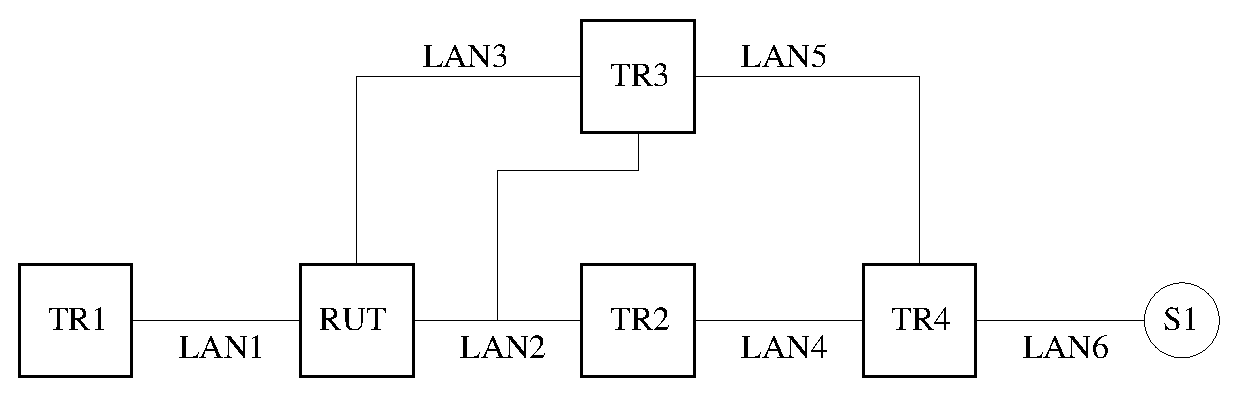
\includegraphics[scale=0.8]{figs/pim_test_5_2_wc_assert_message_state_machine}
    \caption{(*,G) Assert message state machine test setup}
    \label{fig:pim_test_5_2_wc_assert_message_state_machine}
  \end{center}
\end{figure}

\para{Procedure:}

\subpara{Part A: Receive Inferior Assert with RPTbit set and
CouldAssert(*,G,I) in NoInfo state.}

\begin{enumerate}

  \item Start the RUT, TR1, TR2, and TR4. If necessary, wait until the RP-set
  in the RUT, TR1, TR2 and TR4 converges.

  \item Compose an (*,G) Join message at TR1, and send it to the RUT.
  The \verb=J/P_HoldTime= of the message should be set to its default
  value ({\PimsmJPHoldTime}).

  \item Start S1.

  \item Start observing the Assert messages transmitted by the RUT on
  LAN3, and the (*,G) Assert state in the RUT.

  \item Compose an Assert message at TR3 with the S address set to the
  address of S1, the RPT-bit set to one, metric and metric preference set to
  1000, and send it on LAN3.

  \item Start observing the Assert messages transmitted by the RUT on
  LAN1, the (*,G) Assert state in the RUT, and the data packets forwarded on
  LAN1. 

  \item Compose an Assert message at TR1 with the S address set to the
  address of S1, the RPT-bit set to one, metric and metric preference set to
  1000, and send it on LAN1.

  \item Continue observing the Assert messages transmitted by the RUT on
  LAN1, the (*,G) Assert state in the RUT, and the data packets forwarded on
  LAN1.

\end{enumerate}

\subpara{Part B: [This part is intentionally left blank.]}

\subpara{Part C: Data arrives for G on I and
CouldAssert(*,G,I) in NoInfo state.}

\begin{enumerate}

  \item Start the RUT, TR1, TR2, and TR4. If necessary, wait until the RP-set
  in the RUT, TR1, TR2 and TR4 converges.

  \item Compose an (*,G) Join message at TR1, and send it to the RUT.
  The \verb=J/P_HoldTime= of the message should be set to its default
  value ({\PimsmJPHoldTime}).

  \item Start S1.

  \item Start observing the Assert messages transmitted by the RUT on
  LAN1, the (*,G) Assert state in the RUT, and the data packets forwarded on
  LAN1. 

  \item Compose a data packet at TR3 with the S address set to the
  address of S1, and send it on LAN3.

  \item Continue observing the Assert messages transmitted by the RUT on
  LAN1, the (*,G) Assert state in the RUT, and the data packets forwarded on
  LAN1.

  \item Compose a data packet at TR1 with the S address set to the
  address of S1, and send it on LAN1.

  \item Continue observing the Assert messages transmitted by the RUT on
  LAN1, the (*,G) Assert state in the RUT, and the data packets forwarded on
  LAN1.

\end{enumerate}

\subpara{Part D: Receive Preferred Assert with RPTbit set and
AssertTrackingDesired(*,G,I) in NoInfo state.}

\begin{enumerate}

  \item Start the RUT, TR1, TR2, and TR4. If necessary, wait until the RP-set
  in the RUT, TR1, TR2 and TR4 converges.

  \item Compose an (*,G) Join message at TR1, and send it to the RUT.
  The \verb=J/P_HoldTime= of the message should be set to its default
  value ({\PimsmJPHoldTime}).

  \item Start observing the (*,G) Assert state in the RUT.

  \item Compose an Assert message at TR3 with the S address set to the
  address of S1, the RPT-bit set to one, metric and metric preference set to
  10, and send it on LAN3.

  \item Continue observing the (*,G) Assert state in the RUT.

  \item Compose an Assert message at TR1 with the S address set to the
  address of S1, the RPT-bit set to one, metric and metric preference set to
  10, and send it on LAN1.

  \item Continue observing the (*,G) Assert state in the RUT.

  \item Compose an Assert message at TR3 with the S address set to the
  address of S1, the RPT-bit set to one, metric and metric preference set to
  10, and send it on LAN2.

  \item Continue observing the (*,G) Assert state in the RUT.

  \item Compose an (*,G) Join message at TR3, and send it to the RUT on LAN3.
  The \verb=J/P_HoldTime= of the message should be set to its default
  value ({\PimsmJPHoldTime}).

  \item Compose an Assert message at TR3 with the S address set to the
  address of S1, the RPT-bit set to one, metric and metric preference set to
  10, and send it on LAN2.

  \item Continue observing the (*,G) Assert state in the RUT.

\end{enumerate}

\subpara{Part E: Timer expires in I Am Assert Winner state.}

\begin{enumerate}

  \item Start the RUT, TR1, TR2, and TR4. If necessary, wait until the RP-set
  in the RUT, TR1, TR2 and TR4 converges.

  \item Compose an (*,G) Join message at TR1, and send it to the RUT.
  The \verb=J/P_HoldTime= of the message should be set to its default
  value ({\PimsmJPHoldTime}).

  \item Start S1.

  \item Start observing the Assert messages transmitted by the RUT on
  LAN1, the (*,G) Assert state in the RUT, and the data packets forwarded on
  LAN1.

  \item Compose an Assert message at TR1 with the S address set to the
  address of S1, the RPT-bit set to one, metric and metric preference set to
  1000, and send it on LAN1.

  \item Continue observing the Assert messages transmitted by the RUT on
  LAN1, the (*,G) Assert state in the RUT, and the data packets forwarded on
  LAN1 for at least \newline
  (\verb=Assert_Time= - \verb=Assert_Override_Interval=)
  ({\PimsmAssertTime} - {\PimsmAssertOverrideInterval}).
  In the mean time, every \verb=t_periodic= ({\PimsmTPeriodic}) compose same
  (*,G) Join message at TR1, and send it to the RUT.

\end{enumerate}

\subpara{Part F: Receive inferior Assert in I Am Assert Winner state.}

The setup is same as in Part A, except that TR3 does not need to transmit an
Assert message, and that TR1 transmits another Assert
message on LAN1 few seconds after its first Assert message.

\subpara{Part G: Receive Preferred Assert in I Am Assert Winner State.}

\begin{enumerate}

  \item Start the RUT, TR1, TR2, and TR4. If necessary, wait until the RP-set
  in the RUT, TR1, TR2 and TR4 converges.

  \item Compose an (*,G) Join message at TR1, and send it to the RUT.
  The \verb=J/P_HoldTime= of the message should be set to its default
  value ({\PimsmJPHoldTime}).

  \item Start S1.

  \item Start observing the Assert messages transmitted by the RUT on
  LAN1, the (*,G) Assert state in the RUT, and the data packets forwarded on
  LAN1. 

  \item Compose an Assert message at TR1 with the S address set to the
  address of S1, the RPT-bit set to one, metric and metric preference set to
  1000, and send it on LAN1.

  \item Continue observing the Assert messages transmitted by the RUT on
  LAN1, the (*,G) Assert state in the RUT, and the data packets forwarded on
  LAN1.

  \item Compose an Assert message at TR1 with the S address set to the
  address of S1, the RPT-bit set to one, metric and metric preference set to
  10, and send it on LAN1.

  \item Continue observing the Assert messages transmitted by the RUT on
  LAN1, the (*,G) Assert state in the RUT, and the data packets forwarded on
  LAN1.

\end{enumerate}

\subpara{Part H: CouldAssert(*,G,I) $\Longrightarrow$ FALSE transaction
in I Am Assert Winner state.}

\begin{enumerate}

  \item Start the RUT, TR1, TR2, and TR4. If necessary, wait until the RP-set
  in the RUT, TR1, TR2 and TR4 converges.

  \item Compose an (*,G) Join message at TR1, and send it to the RUT.
  The \verb=J/P_HoldTime= of the message should be set to its default
  value ({\PimsmJPHoldTime}).

  \item Compose an (*,G) Join message at TR3, and send it to the RUT on LAN3.
  The \verb=J/P_HoldTime= of the message should be set to its default
  value ({\PimsmJPHoldTime}).

  \item Start S1.

  \item Start observing the Assert messages transmitted by the RUT on
  LAN1, the (*,G) Assert state in the RUT, and the data packets forwarded on
  LAN1. 

  \item Compose an Assert message at TR1 with the S address set to the
  address of S1, the RPT-bit set to one, metric and metric preference set to
  1000, and send it on LAN1.

  \item Continue observing the Assert messages transmitted by the RUT on
  LAN1, the (*,G) Assert state in the RUT, and the data packets forwarded on
  LAN1.

  \item Compose an (*,G) Prune message at TR1, and send it to the RUT.
  The \verb=J/P_HoldTime= of the message should be set to its default
  value ({\PimsmJPHoldTime}).

  \item Continue observing the Assert messages transmitted by the RUT on
  LAN1, the (*,G) Assert state in the RUT, and the data packets forwarded on
  LAN1.

\end{enumerate}

\subpara{Part I: Receive Preferred Assert in I Am Assert Loser State.}

\begin{enumerate}

  \item Start the RUT, TR1, TR2, and TR4. If necessary, wait until the RP-set
  in the RUT, TR1, TR2 and TR4 converges.

  \item Compose an (*,G) Join message at TR1, and send it to the RUT.
  The \verb=J/P_HoldTime= of the message should be set to its default
  value ({\PimsmJPHoldTime}).

  \item Start S1.

  \item Start observing the Assert messages transmitted by the RUT on
  LAN1, the (*,G) Assert state in the RUT, and the data packets forwarded on
  LAN1.

  \item Compose an Assert message at TR1 with the S address set to the
  address of S1, the RPT-bit set to one, metric and metric preference set to
  10, and send it on LAN1.

  \item Continue observing the Assert messages transmitted by the RUT on
  LAN1, the (*,G) Assert state in the RUT, and the data packets forwarded on
  LAN1.

  \item Compose an Assert message at TR1 with the S address set to the
  address of S1, the RPT-bit set to one, metric and metric preference set to
  1, and send it on LAN1.

  \item Continue observing the Assert messages transmitted by the RUT on
  LAN1, the (*,G) Assert state in the RUT, and the data packets forwarded on
  LAN1.

\end{enumerate}

\subpara{Part J: Receive Acceptable Assert from Current Winner in I Am Assert
Loser State.}

The setup is same as in Part I, except that the second Assert message that TR1
transmits on LAN1 should have metric and metric preference set to 50.

\subpara{Part K: Receive Inferior Assert from Current Winner in I Am Assert
Loser State.}

The setup is same as in Part I, except that the second Assert message that TR1
transmits on LAN1 should have metric and metric preference set to 1000.

\subpara{Part L: Timer expires in I Am Assert Loser State.}

\begin{enumerate}

  \item Start the RUT, TR1, TR2, and TR4. If necessary, wait until the RP-set
  in the RUT, TR1, TR2 and TR4 converges.

  \item Compose an (*,G) Join message at TR1, and send it to the RUT.
  The \verb=J/P_HoldTime= of the message should be set to its default
  value ({\PimsmJPHoldTime}).

  \item Start S1.

  \item Start observing the Assert messages transmitted by the RUT on
  LAN1, the (*,G) Assert state in the RUT, and the data packets forwarded on
  LAN1.

  \item Compose an Assert message at TR1 with the S address set to the
  address of S1, the RPT-bit set to one, metric and metric preference set to
  10, and send it on LAN1.

  \item Continue observing the Assert messages transmitted by the RUT on
  LAN1, the (*,G) Assert state in the RUT, and the data packets forwarded on
  LAN1 for at least (\verb=Assert_Time=) ({\PimsmAssertTime}).

\end{enumerate}

\subpara{Part M: Current winner's GenID changes in I Am Assert Loser State.}

\begin{enumerate}

  \item Start the RUT, TR1, TR2, and TR4. If necessary, wait until the RP-set
  in the RUT, TR1, TR2 and TR4 converges.

  \item Compose an (*,G) Join message at TR1, and send it to the RUT.
  The \verb=J/P_HoldTime= of the message should be set to its default
  value ({\PimsmJPHoldTime}).

  \item Start S1.

  \item Start observing the Assert messages transmitted by the RUT on
  LAN1, the (*,G) Assert state in the RUT, and the data packets forwarded on
  LAN1.

  \item Compose an Assert message at TR1 with the S address set to the
  address of S1, the RPT-bit set to one, metric and metric preference set to
  10, and send it on LAN1.

  \item Continue observing the Assert messages transmitted by the RUT on
  LAN1, the (*,G) Assert state in the RUT, and the data packets forwarded on
  LAN1.

  \item Quit TR1 (\ie stop it without graceful shutdown), and start it
  immediately.

  \item Continue observing the Assert messages transmitted by the RUT on
  LAN1, the (*,G) Assert state in the RUT, and the data packets forwarded on
  LAN1.

\end{enumerate}

\subpara{Part N: AssertTrackingDesired(*,G,I)  $\Longrightarrow$ FALSE
transaction in I Am Assert Loser State.}

\begin{enumerate}

  \item Start the RUT, TR1, TR2, and TR4. If necessary, wait until the RP-set
  in the RUT, TR1, TR2 and TR4 converges.

  \item Compose an (*,G) Join message at TR1, and send it to the RUT.
  The \verb=J/P_HoldTime= of the message should be set to its default
  value ({\PimsmJPHoldTime}).

  \item Start S1.

  \item Start observing the Assert messages transmitted by the RUT on
  LAN1 and LAN2, the (*,G) Assert state in the RUT, and the data packets
  forwarded on LAN1.

  \item Compose an Assert message at TR3 with the S address set to the
  address of S1, the RPT-bit set to one, metric and metric preference set to
  10, and send it on LAN2.

  \item Continue observing the Assert messages transmitted by the RUT on
  LAN1 and LAN2, the (*,G) Assert state in the RUT, and the data packets
  forwarded on LAN1.

  \item Compose an Assert message at TR1 with the S address set to the
  address of S1, the RPT-bit set to one, metric and metric preference set to
  10, and send it on LAN1.

  \item Continue observing the Assert messages transmitted by the RUT on
  LAN1 and LAN2, the (*,G) Assert state in the RUT, and the data packets
  forwarded on LAN1.

  \item Compose an (*,G) Join message at TR3, and send it to the RUT on LAN2.
  The \verb=J/P_HoldTime= of the message should be set to its default
  value ({\PimsmJPHoldTime}).

  \item Compose an (*,G) Prune message at TR1, and send it to the RUT.
  The \verb=J/P_HoldTime= of the message should be set to its default
  value ({\PimsmJPHoldTime}).

  \item Continue observing the Assert messages transmitted by the RUT on
  LAN1 and LAN2, the (*,G) Assert state in the RUT, and the data packets
  forwarded on LAN1.

\end{enumerate}

\subpara{Part O: my\_assert\_metric $\Longrightarrow$ better than winner's
metric in I Am Assert Loser State.}

\begin{enumerate}

  \item Start the RUT, TR1, TR2, and TR4. If necessary, wait until the RP-set
  in the RUT, TR1, TR2 and TR4 converges.

  \item Compose an (*,G) Join message at TR1, and send it to the RUT.
  The \verb=J/P_HoldTime= of the message should be set to its default
  value ({\PimsmJPHoldTime}).

  \item Compose an (*,G) Join message at TR3, and send it to the RUT on LAN3.
  The \verb=J/P_HoldTime= of the message should be set to its default
  value ({\PimsmJPHoldTime}).

  \item Start S1.

  \item Start observing the Assert messages transmitted by the RUT on
  LAN1, the (*,G) Assert state in the RUT, and the data packets forwarded on
  LAN1.

  \item Compose an Assert message at TR1 with the S address set to the
  address of S1, the RPT-bit set to one, metric and metric preference set to
  10, and send it on LAN1.

  \item Continue observing the Assert messages transmitted by the RUT on
  LAN1, the (*,G) Assert state in the RUT, and the data packets forwarded on
  LAN1.

  \item Reconfigure the MRIB in the RUT, such that MRIB.pref(RP(G)) = 1, and
  MRIB.metric(RP(G)) = 1.

  \item Continue observing the Assert messages transmitted by the RUT on
  LAN1, the (*,G) Assert state in the RUT, and the data packets forwarded on
  LAN1.

  \item Repeat the test with MRIB.pref(RP(G)) = 50,
  and MRIB.metric(RP(G)) = 50.

\end{enumerate}

\subpara{Part P: RPF\_interface(RP(G)) stops being I in I Am Assert Loser
State.}

\begin{enumerate}

  \item Start the RUT, TR1, TR2, and TR4. If necessary, wait until the RP-set
  in the RUT, TR1, TR2 and TR4 converges.

  \item Compose an (*,G) Join message at TR1, and send it to the RUT.
  The \verb=J/P_HoldTime= of the message should be set to its default
  value ({\PimsmJPHoldTime}).

  \item Start S1.

  \item Start observing the Assert messages transmitted by the RUT on
  LAN2 and LAN3, the (*,G) Assert state in the RUT, and the data packets
  forwarded on LAN1.

  \item Compose an Assert message at TR3 with the S address set to the
  address of S1, the RPT-bit set to one, metric and metric preference set to
  10, and send it on LAN2.

  \item Continue observing the Assert messages transmitted by the RUT on
  LAN2 and LAN3, the (*,G) Assert state in the RUT, and the data packets
  forwarded on LAN1.

  \item Reconfigure the RPF information in the RUT, such that
  RPF\_interface(RP(G)) is the interface that connects the RUT to LAN3.

  \item Continue observing the Assert messages transmitted by the RUT on
  LAN2 and LAN3, the (*,G) Assert state in the RUT, and the data packets
  forwarded on LAN1.

\end{enumerate}

\subpara{Part Q: Receive Join(*,G) or Join(*,*,RP(G)) on interface I in I Am
Assert Loser State.}

\begin{enumerate}

  \item Start the RUT, TR1, TR2, and TR4. If necessary, wait until the RP-set
  in the RUT, TR1, TR2 and TR4 converges.

  \item Compose an (*,G) Join message at TR1, and send it to the RUT.
  The \verb=J/P_HoldTime= of the message should be set to its default
  value ({\PimsmJPHoldTime}).

  \item Start S1.

  \item Start observing the Assert messages transmitted by the RUT on
  LAN1, the (*,G) Assert state in the RUT, and the data packets forwarded on
  LAN1. 

  \item Compose an Assert message at TR1 with the S address set to the
  address of S1, the RPT-bit set to one, metric and metric preference set to
  10, and send it on LAN1.

  \item Continue observing the Assert messages transmitted by the RUT on
  LAN1, the (*,G) Assert state in the RUT, and the data packets forwarded on
  LAN1.

  \item Compose an (*,G) Join message at TR1, and send it to the RUT.
  The \verb=J/P_HoldTime= of the message should be set to its default
  value ({\PimsmJPHoldTime}).

  \item Continue observing the Assert messages transmitted by the RUT on
  LAN1, the (*,G) Assert state in the RUT, and the data packets forwarded on
  LAN1.

  \item Repeat the test except that TR1 composes and sends (*,*,RP) Join
  message instead of the second (*,G) Join message.

\end{enumerate}

\subpara{Part R: (*,G) assert state machine suppressed by (S,G) assert state
machine.}

\begin{enumerate}

  \item Start the RUT, TR1, TR2, and TR4. If necessary, wait until the RP-set
  in the RUT, TR1, TR2 and TR4 converges.

  \item Compose an (*,G) Join message at TR1, and send it to the RUT.
  The \verb=J/P_HoldTime= of the message should be set to its default
  value ({\PimsmJPHoldTime}).

  \item Compose an (S,G) Join message at TR1 with the S address set to the
  address of S1, and send it to the RUT.
  The \verb=J/P_HoldTime= of the message should be set to its default
  value ({\PimsmJPHoldTime}).

  \item Start S1.

  \item Start observing the Assert messages transmitted by the RUT on
  LAN1, the (S,G) and (*,G) Assert state in the RUT, and the data packets
  forwarded on LAN1. 

  \item Compose an Assert message at TR1 with the S address set to the
  address of S1, the RPT-bit set to zero, metric and metric preference set to
  10, and send it on LAN1.

  \item Continue observing the Assert messages transmitted by the RUT on
  LAN1, the (S,G) and (*,G) Assert state in the RUT, and the data packets
  forwarded on LAN1.

  \item Compose an Assert message at TR1 with the S address set to the
  address of S1, the RPT-bit set to one, metric and metric preference set to
  1000, and send it on LAN1.

  \item Continue observing the Assert messages transmitted by the RUT on
  LAN1, the (S,G) and (*,G) Assert state in the RUT, and the data packets
  forwarded on LAN1.

\end{enumerate}

\subpara{Part S: (*,G) assert state machine not suppressed by (S,G) assert
state machine.}

\begin{enumerate}

  \item Start the RUT, TR1, TR2, and TR4. If necessary, wait until the RP-set
  in the RUT, TR1, TR2 and TR4 converges.

  \item Compose an (*,G) Join message at TR1, and send it to the RUT.
  The \verb=J/P_HoldTime= of the message should be set to its default
  value ({\PimsmJPHoldTime}).

  \item Compose an (S,G) Join message at TR3 with the S address set to the
  address of S1, and send it to the RUT on LAN3.
  The \verb=J/P_HoldTime= of the message should be set to its default
  value ({\PimsmJPHoldTime}).

  \item Compose an (S,G,rpt) Prune message at TR1, and send it to the RUT.
  The \verb=J/P_HoldTime= of the message should be set to its default
  value ({\PimsmJPHoldTime}).

  \item Start S1.

  \item Start observing the Assert messages transmitted by the RUT on
  LAN1, the (S,G) and (*,G) Assert state in the RUT, and the data packets
  forwarded on LAN1. 

  \item Compose an Assert message at TR1 with the S address set to the
  address of S1, the RPT-bit set to one, metric and metric preference set to
  10, and send it on LAN1.

  \item Continue observing the Assert messages transmitted by the RUT on
  LAN1, the (S,G) and (*,G) Assert state in the RUT, and the data packets
  forwarded on LAN1.

  \item Compose an Assert message at TR1 with the S address set to the
  address of S1, the RPT-bit set to one, metric and metric preference set to
  1000, and send it on LAN1.

  \item Continue observing the Assert messages transmitted by the RUT on
  LAN1, the (S,G) and (*,G) Assert state in the RUT, and the data packets
  forwarded on LAN1.

\end{enumerate}


\para{Observable Results:}

\subpara{Part A:}

\begin{itemize}

  \item After TR1 sends the (*,G) Join message to the RUT, the interface that
  connects the RUT to LAN1 should be added to the set of joined interfaces for
  the corresponding (*,G) routing state; the incoming interface for that state
  should be the interface that connects the RUT to LAN2.

  \item After S1 is started, the data packets should be forwarded on LAN1.

  \item After TR3 transmits the Assert message on LAN3, the (*,G) Assert state
  machine for the interface that connects the RUT to LAN3 should continue to
  be in NoInfo state.

  \item After TR1 transmits the Assert message on LAN1, the RUT itself should
  transmit an (*,G) Assert message on LAN1 with the RPT bit set to one,
  and the metric and metric preference set to 100. The (*,G) Assert state
  machine for the interface that connects the RUT to LAN1 should be in I Am
  Assert Winner state:

\begin{verbatim}
Xorp> show pim join 
Group           Source          RP              Flags
224.0.1.20      0.0.0.0         10.4.0.1        WC   
    Upstream interface (RP):   dc1
    Upstream MRIB next hop (RP): 10.2.0.2
    Upstream RPF'(*,G):        10.2.0.2
    Upstream state:            Joined 
    Join timer:                9
    Local receiver include WC: ..............
    Joins RP:                  ..............
    Joins WC:                  ........O.....
    Join state:                ........O.....
    Prune state:               ..............
    Prune pending state:       ..............
    I am assert winner state:  ........O.....
    I am assert loser state:   ..............
    Assert winner WC:          ........O.....
    Assert lost WC:            ..............
    Assert tracking WC:        .....O..O.....
    Could assert WC:           ........O.....
    I am DR:                   ........O.....
    Immediate olist RP:        ..............
    Immediate olist WC:        ........O.....
    Inherited olist SG:        ..............
    Inherited olist SG_RPT:    ..............
    PIM include WC:            ..............
\end{verbatim}

  In addition, the RUT should store self as AssertWinner(*,G,I), it should
  store rpt\_assert\_metric(G,I) as AssertWinnerMetric(*,G,I), and the
  Assert Timer should be set to \newline
  (\verb=Assert_Time= - \verb=Assert_Override_Interval=)
  ({\PimsmAssertTime} - {\PimsmAssertOverrideInterval}).
  After that, the RUT should continue to forward the data packets from S1 on
  LAN1.

\end{itemize}

\subpara{Part B:}

[This part is intentionally left blank].

\subpara{Part C:}

The results should be same as in Part A, except that the Assert message
transmitted by the RUT is triggered by the data packet.

\subpara{Part D:}

\begin{itemize}

  \item After TR1 sends the (*,G) Join message to the RUT, the interface that
  connects the RUT to LAN1 should be added to the set of joined interfaces for
  the corresponding (*,G) routing state; the incoming interface for that state
  should be the interface that connects the RUT to LAN2.

  \item After TR3 transmits the Assert message on LAN3, the (*,G) Assert state
  machine for the interface that connects the RUT to LAN3 should continue to
  be in NoInfo state.

  \item After TR1 transmits the Assert message on LAN1, the (*,G) Assert state
  machine for the interface that connects the RUT to LAN1 should be in I Am
  Assert Loser state:

\begin{verbatim}
Xorp> show pim join 
Group           Source          RP              Flags
224.0.1.20      0.0.0.0         10.4.0.1        WC   
    Upstream interface (RP):   dc1
    Upstream MRIB next hop (RP): 10.2.0.2
    Upstream RPF'(*,G):        10.2.0.2
    Upstream state:            NotJoined 
    Join timer:                -1
    Local receiver include WC: ..............
    Joins RP:                  ..............
    Joins WC:                  ........O.....
    Join state:                ........O.....
    Prune state:               ..............
    Prune pending state:       ..............
    I am assert winner state:  ..............
    I am assert loser state:   ........O.....
    Assert winner WC:          ..............
    Assert lost WC:            ........O.....
    Assert tracking WC:        ........O.....
    Could assert WC:           ........O.....
    I am DR:                   ........O.....
    Immediate olist RP:        ..............
    Immediate olist WC:        ..............
    Inherited olist SG:        ..............
    Inherited olist SG_RPT:    ..............
    PIM include WC:            ..............
\end{verbatim}

  In addition, the RUT should store TR1 as AssertWinner(*,G,I) for the
  interface that connects the RUT to LAN1, it should store the assert metric
  of TR1 as AssertWinnerMetric(*,G,I), and the Assert Timer should be set to
  (\verb=Assert_Time=) ({\PimsmAssertTime}).

  \item After TR3 transmits the first Assert message on LAN2, the (*,G) Assert
  state machine for the interface that connects the RUT to LAN2 should
  continue to be in NoInfo state.

  \item After TR3 transmits the second Assert message on LAN2, the (*,G) Assert
  state machine for the interface that connects the RUT to LAN2 should be in I
  Am Assert Loser state. In addition,
  the RPF'(*,G) should be set to the interface that connects TR3
  to LAN2:

\begin{verbatim}
Xorp> show pim join 
Group           Source          RP              Flags
224.0.1.20      0.0.0.0         10.4.0.1        WC   
    Upstream interface (RP):   dc1
    Upstream MRIB next hop (RP): 10.2.0.2
    Upstream RPF'(*,G):        10.2.0.4
    Upstream state:            Joined 
    Join timer:                59
    Local receiver include WC: ..............
    Joins RP:                  ..............
    Joins WC:                  ......O.O.....
    Join state:                ......O.O.....
    Prune state:               ..............
    Prune pending state:       ..............
    I am assert winner state:  ..............
    I am assert loser state:   .....O..O.....
    Assert winner WC:          ..............
    Assert lost WC:            ........O.....
    Assert tracking WC:        .....OO.O.....
    Could assert WC:           ......O.O.....
    I am DR:                   ........O.....
    Immediate olist RP:        ..............
    Immediate olist WC:        ......O.......
    Inherited olist SG:        ..............
    Inherited olist SG_RPT:    ..............
    PIM include WC:            ..............
\end{verbatim}

  In addition, the RUT should store TR3 as AssertWinner(*,G,I) for the
  interface that connects the RUT to LAN2, it should store the assert metric
  of TR3 as AssertWinnerMetric(*,G,I), and the Assert Timer should be set to
  (\verb=Assert_Time=) ({\PimsmAssertTime}).

\end{itemize}

\subpara{Part E:}

\begin{itemize}

  \item Until after the RUT receives the Assert message from TR1, the results
  should be same as in Part A. After that, once every \newline
  (\verb=Assert_Time= - \verb=Assert_Override_Interval=)
  ({\PimsmAssertTime} - {\PimsmAssertOverrideInterval}).
  the RUT should transmit an Assert message on LAN1 with the RPT bit set to
  one, the metric and metric preference set to 100. The (*,G) Assert state
  machine for the interface that connects the RUT to LAN1 should continue to
  be in I Am Assert Winner state.

\end{itemize}

\subpara{Part F:}

\begin{itemize}

  \item Until after the RUT receives the first Assert message from TR1, the
  results should be same as in Part A.

  \item After the RUT receives the second Assert message from TR1, the RUT
  the RUT should transmit Assert an message on LAN1 with the RPT bit set to
  one, the metric and metric preference set to 100. The (*,G) Assert state
  machine for the interface that connects the RUT to LAN1 should continue to
  be in I Am Assert Winner state. In addition, the Assert Timer should be set
  to \newline
  (\verb=Assert_Time= - \verb=Assert_Override_Interval=)
  ({\PimsmAssertTime} - {\PimsmAssertOverrideInterval}).

\end{itemize}

\subpara{Part G:}

\begin{itemize}

  \item Until after the RUT receives the first Assert message from TR1, the
  results should be same as in Part A.

  \item After the RUT receives the second Assert message from TR1, the (*,G)
  Assert state machine for the interface that connects the RUT to LAN1 should
  be in I Am Assert Loser state:

\begin{verbatim}
Xorp> show pim join 
Group           Source          RP              Flags
224.0.1.20      0.0.0.0         10.4.0.1        WC   
    Upstream interface (RP):   dc1
    Upstream MRIB next hop (RP): 10.2.0.2
    Upstream RPF'(*,G):        10.2.0.2
    Upstream state:            NotJoined 
    Join timer:                -1
    Local receiver include WC: ..............
    Joins RP:                  ..............
    Joins WC:                  ........O.....
    Join state:                ........O.....
    Prune state:               ..............
    Prune pending state:       ..............
    I am assert winner state:  ..............
    I am assert loser state:   ........O.....
    Assert winner WC:          ..............
    Assert lost WC:            ........O.....
    Assert tracking WC:        ........O.....
    Could assert WC:           ........O.....
    I am DR:                   ........O.....
    Immediate olist RP:        ..............
    Immediate olist WC:        ..............
    Inherited olist SG:        ..............
    Inherited olist SG_RPT:    ..............
    PIM include WC:            ..............
\end{verbatim}

  In addition, the RUT should store TR1 as AssertWinner(*,G,I) for the
  interface that connects the RUT to LAN1, it should store the assert metric
  of TR1 as AssertWinnerMetric(*,G,I), and the Assert Timer should be set to
  (\verb=Assert_Time=) ({\PimsmAssertTime}).
  Further, it should stop forwarding the data packets from S1 on LAN1.

\end{itemize}

\subpara{Part H:}

\begin{itemize}

  \item Until after the RUT receives the Assert message from TR1, the results
  should be similar as in Part A, except that the interface that connects the
  RUT to LAN3 should also be added to the set of (*,G) Joined interfaces, and
  to the set of outgoing interfaces:

\begin{verbatim}
Xorp> show pim join 
Group           Source          RP              Flags
224.0.1.20      0.0.0.0         10.4.0.1        WC   
    Upstream interface (RP):   dc1
    Upstream MRIB next hop (RP): 10.2.0.2
    Upstream RPF'(*,G):        10.2.0.2
    Upstream state:            Joined 
    Join timer:                40
    Local receiver include WC: ..............
    Joins RP:                  ..............
    Joins WC:                  ......O.O.....
    Join state:                ......O.O.....
    Prune state:               ..............
    Prune pending state:       ..............
    I am assert winner state:  ..............
    I am assert loser state:   ..............
    Assert winner WC:          ..............
    Assert lost WC:            ..............
    Assert tracking WC:        .....OO.O.....
    Could assert WC:           ......O.O.....
    I am DR:                   ........O.....
    Immediate olist RP:        ..............
    Immediate olist WC:        ......O.O.....
    Inherited olist SG:        ..............
    Inherited olist SG_RPT:    ..............
    PIM include WC:            ..............
\end{verbatim}

  \item After TR1 transmits the (*,G) Prune message to the RUT, the (*,G)
  Assert state machine for the interface that connects the RUT to LAN1 should
  be in NoInfo state:

\begin{verbatim}
Xorp> show pim join 
Group           Source          RP              Flags
224.0.1.20      0.0.0.0         10.4.0.1        WC   
    Upstream interface (RP):   dc1
    Upstream MRIB next hop (RP): 10.2.0.2
    Upstream RPF'(*,G):        10.2.0.2
    Upstream state:            Joined 
    Join timer:                11
    Local receiver include WC: ..............
    Joins RP:                  ..............
    Joins WC:                  ......O.......
    Join state:                ......O.......
    Prune state:               ..............
    Prune pending state:       ..............
    I am assert winner state:  ..............
    I am assert loser state:   ..............
    Assert winner WC:          ..............
    Assert lost WC:            ..............
    Assert tracking WC:        .....OO.......
    Could assert WC:           ......O.......
    I am DR:                   ........O.....
    Immediate olist RP:        ..............
    Immediate olist WC:        ......O.......
    Inherited olist SG:        ..............
    Inherited olist SG_RPT:    ..............
    PIM include WC:            ..............
\end{verbatim}

  The RUT should send AssertCancel(*,G) on LAN1 (\ie an (*,G) Assert message
  with the source address set to RP(G), the RPT bit set to one, the metric set
  to 0xffffffff, and the metric preference set to 0x7fffffff).
  Further, the RUT should delete the AssertWinner(*,G,I) and
  AssertWinnerMetric(*,G,I) information for the interface that connects it to
  LAN1.
  In addition, the RUT should stop forwarding the data packets from S1 on LAN1.

\end{itemize}

\subpara{Part I:}

\begin{itemize}

  \item After TR1 sends the (*,G) Join message to the RUT, the interface that
  connects the RUT to LAN1 should be added to the set of joined interfaces for
  the corresponding (*,G) routing state; the incoming interface for that state
  should be the interface that connects the RUT to LAN2.

  \item After S1 is started, the data packets should be forwarded on LAN1.

  \item After the RUT receives the first Assert message from TR1, the (*,G)
  Assert state machine for the interface that connects the RUT to LAN1 should
  be in I Am Assert Loser state.

  In addition, the RUT should store TR1 as AssertWinner(*,G,I) for the
  interface that connects the RUT to LAN1, it should store the assert metric
  of TR1 as AssertWinnerMetric(*,G,I), and the Assert Timer should be set to
  (\verb=Assert_Time=) ({\PimsmAssertTime}).
  Further, it should stop forwarding the data packets from S1 on LAN1.

  \item After the RUT receives the second Assert message from TR1, the (*,G)
  Assert state machine for the interface that connects the RUT to LAN1 should
  continue to be in I Am Assert Loser state.

  In addition, the RUT should store TR1 as AssertWinner(*,G,I) for the
  interface that connects the RUT to LAN1, it should store the new assert
  metric of TR1 as AssertWinnerMetric(*,G,I), and the Assert Timer should be
  set to (\verb=Assert_Time=) ({\PimsmAssertTime}).

\end{itemize}

\subpara{Part J:}

The results should be same as in Part I.

\subpara{Part K:}

\begin{itemize}

  \item Until after the RUT receives the first Assert message from TR1, the
  results should be same as in Part I.

  \item After the RUT receives the second Assert message from TR1, the (*,G)
  Assert state machine for the interface that connects the RUT to LAN1 should
  be in NoInfo state.
  Further, the RUT should delete the AssertWinner(*,G,I) and
  AssertWinnerMetric(*,G,I) information for the interface that connects it to
  LAN1.
  In addition, the RUT should start forwarding the data packets from S1 on
  LAN1.

\end{itemize}

\subpara{Part L:}

\begin{itemize}

  \item Until after the RUT receives the first Assert message from TR1, the
  results should be same as in Part I.

  \item The (*,G) Assert state machine for the interface that connects the RUT
  to LAN1 should continue to be in I Am Assert Loser state for
  (\verb=Assert_Time=) ({\PimsmAssertTime}). After that the Assert Timer for
  that interface should expire, and the assert state machine should be in No
  Info state.
  Further, the RUT should delete the AssertWinner(*,G,I) and
  AssertWinnerMetric(*,G,I) information for the interface that connects it to
  LAN1.
  In addition, the RUT should start forwarding the data packets from S1 on
  LAN1.

\end{itemize}

\subpara{Part M:}

\begin{itemize}

  \item Until after the RUT receives the first Assert message from TR1, the
  results should be same as in Part I.

  \item After TR1 is restarted and the RUT has received the first Hello
  message from it, the (*,G) Assert state machine for the
  interface that connects the RUT to LAN1 should be in NoInfo state.
  Further, the RUT should delete the AssertWinner(*,G,I) and
  AssertWinnerMetric(*,G,I) information for the interface that connects it to
  LAN1.
  In addition, the RUT should start forwarding the data packets from S1 on
  LAN1.

\end{itemize}

\subpara{Part N:}

\begin{itemize}

  \item After TR1 sends the (*,G) Join message to the RUT, the interface that
  connects the RUT to LAN1 should be added to the set of joined interfaces for
  the corresponding (*,G) routing state; the incoming interface for that state
  should be the interface that connects the RUT to LAN2.

  \item After S1 is started, the data packets should be forwarded on LAN1.

  \item After the RUT receives the Assert message from TR3, the (*,G)
  Assert state machine for the interface that connects the RUT to LAN2 should
  be in I Am Assert Loser state.

  In addition, the RUT should store TR3 as AssertWinner(*,G,I) for the
  interface that connects the RUT to LAN2, it should store the assert metric
  of TR3 as AssertWinnerMetric(*,G,I), and the Assert Timer should be set to
  (\verb=Assert_Time=) ({\PimsmAssertTime}).
  The data packets from S1 should continue to be forwarded on LAN1.

  \item After the RUT receives the Assert message from TR1, the (*,G)
  Assert state machine for the interface that connects the RUT to LAN1 should
  be in I Am Assert Loser state.

  In addition, the RUT should store TR1 as AssertWinner(*,G,I) for the
  interface that connects the RUT to LAN1, it should store the assert metric
  of TR1 as AssertWinnerMetric(*,G,I), and the Assert Timer should be set to
  (\verb=Assert_Time=) ({\PimsmAssertTime}).
  Further, it should stop forwarding the data packets from S1 on LAN1.

  Also, the (*,G) Assert state machine for the interface that connects the RUT
  to LAN2 should be in NoInfo state, and the RUT should delete the
  AssertWinner(*,G,I) and AssertWinnerMetric(*,G,I) information for the
  interface that connects it to LAN2.

  \item After the RUT receives the (*,G) Prune message from TR1, the (*,G)
  Assert state machine for the interface that connects the RUT to LAN1 should
  be in NoInfo state.
  Further, the RUT should delete the AssertWinner(*,G,I) and
  AssertWinnerMetric(*,G,I) information for the interface that connects it to
  LAN1.

\end{itemize}

\subpara{Part O:}

\begin{itemize}

  \item After the RUT receives the (*,G) Join messages from TR1 and TR3, the
  interfaces that connect the RUT to LAN1 and LAN3 respectively should be
  added to the set of joined interfaces for the corresponding (*,G) routing
  state; the incoming interface for that state should be the interface that
  connects the RUT to LAN2.

  \item After S1 is started, the data packets should be forwarded on LAN1 and
  LAN3.

  \item After the RUT receives the Assert message from TR1, the (*,G)
  Assert state machine for the interface that connects the RUT to LAN1 should
  be in I Am Assert Loser state.

  In addition, the RUT should store TR1 as AssertWinner(*,G,I) for the
  interface that connects the RUT to LAN1, it should store the assert metric
  of TR1 as AssertWinnerMetric(*,G,I), and the Assert Timer should be set to
  (\verb=Assert_Time=) ({\PimsmAssertTime}).
  Further, it should stop forwarding the data packets from S1 on LAN1.

  \item After the MRIB in the RUT is reconfigured, the (*,G)
  Assert state machine for the interface that connects the RUT to LAN1 should
  be in NoInfo state.
  Further, the RUT should delete the AssertWinner(*,G,I) and
  AssertWinnerMetric(*,G,I) information for the interface that connects it to
  LAN1.
  In addition, the RUT should start forwarding the data packets from S1 on
  LAN1.

  \item After the test is repeated with MRIB.pref(RP(G)) = 50
  and MRIB.metric(RP(G)) = 50, the Assert state machine for the interface that
  connects the RUT to LAN1 should continue to be in I Am Assert Loser State.

\end{itemize}

\subpara{Part P:}

\begin{itemize}

  \item Until after the RUT receives the Assert message from TR3, the
  results should be same as in Part N.

  \item After RPF\_interface(S) in the RUT is changed, the (*,G)
  Assert state machine for the interface that connects the RUT to LAN2 should
  be in NoInfo state.
  Further, the RUT should delete the AssertWinner(*,G,I) and
  AssertWinnerMetric(*,G,I) information for the interface that connects it to
  LAN1.

\end{itemize}

\subpara{Part Q:}

\begin{itemize}

  \item Until after the RUT receives the Assert message from TR1, the
  results should be same as in Part I.

  \item After the RUT receives the (*,G) Join message from TR1, the (*,G)
  Assert state machine for the interface that connects the RUT to LAN1 should
  be in NoInfo state.
  Further, the RUT should delete the AssertWinner(*,G,I) and
  AssertWinnerMetric(*,G,I) information for the interface that connects it to
  LAN1.
  In addition, the RUT should start forwarding the data packets from S1 on
  LAN1.

  \item When the test is repeated with (*,*,RP) Join message instead of the
  second (*,G) Join messages, the result should be same.

\end{itemize}

\subpara{Part R:}

\begin{itemize}

  \item After the RUT receives the (*,G) and (S,G) Join messages from TR1, the
  interface that connects the RUT to LAN1 should be
  added to the set of joined interfaces for the corresponding (*,G) and (S,G)
  routing states; the incoming interface for those states should be the
  interface that connects the RUT to LAN2.

  \item After S1 is started, the data packets should be forwarded on LAN1.

  \item After the RUT receives the first Assert message from TR1, the (S,G)
  Assert state machine for the interface that connects the RUT to LAN1 should
  be in I Am Assert Loser state. The (*,G) Assert state machine for the
  interface that connects the RUT to LAN1 should continue to be in NoInfo
  state.

  In addition, the RUT should store TR1 as AssertWinner(S,G,I) for the
  interface that connects the RUT to LAN1, it should store the assert metric
  of TR1 as AssertWinnerMetric(S,G,I), and the Assert Timer should be set to
  (\verb=Assert_Time=) ({\PimsmAssertTime}).
  Further, it should stop forwarding the data packets from S1 on LAN1.

  \item After the RUT receives the second Assert message from TR1, the (S,G)
  Assert state machine for the interface that connects the RUT to LAN1 should
  be in NoInfo state. The (*,G) Assert state machine for the
  interface that connects the RUT to LAN1 should continue to be in NoInfo
  state.
  Further, the RUT should delete the AssertWinner(S,G,I) and
  AssertWinnerMetric(S,G,I) information for the interface that connects it to
  LAN1.
  In addition, the RUT should start forwarding the data packets from S1 on
  LAN1.

\end{itemize}

\subpara{Part S:}

\begin{itemize}

  \item After the RUT receives the (*,G) Join message from TR1, the
  interface that connects the RUT to LAN1 should be
  added to the set of joined interfaces for the corresponding (*,G)
  routing state; the incoming interface for that state should be the
  interface that connects the RUT to LAN2.

  \item After the RUT receives the (S,G) Join message from TR3, the
  interface that connects the RUT to LAN3 should be
  added to the set of joined interfaces for the corresponding (S,G)
  routing state; the incoming interface for that state should be the
  interface that connects the RUT to LAN2.

  \item After the RUT receives the (S,G,rpt) Prune message from TR1, the
  interface that connects the RUT to LAN1 should be
  added to the set of prune interfaces for the corresponding (S,G,rpt)
  routing state; the incoming interface for that state should be the
  interface that connects the RUT to LAN2.

  \item After S1 is started, the data packets should be forwarded on LAN3, but
  not on LAN1.

  \item After the RUT receives the first Assert message from TR1, the (*,G)
  Assert state machine for the interface that connects the RUT to LAN1 should
  be in I Am Assert Loser state.

  In addition, the RUT should store TR1 as AssertWinner(*,G,I) for the
  interface that connects the RUT to LAN1, it should store the assert metric
  of TR1 as AssertWinnerMetric(*,G,I), and the Assert Timer should be set to
  (\verb=Assert_Time=) ({\PimsmAssertTime}).

  \item After the RUT receives the second Assert message from TR1, the (*,G)
  Assert state machine for the interface that connects the RUT to LAN1 should
  be in NoInfo state.
  Further, the RUT should delete the AssertWinner(*,G,I) and
  AssertWinnerMetric(*,G,I) information for the interface that connects it to
  LAN1.

\end{itemize}

\para{Possible Problems:}
In Part C, TR1 may transmit two identical Assert messages on LAN1 instead of
one message. Strictly speaking, according to the PIM-SM spec
(draft-ietf-pim-sm-v2-new-05), a router would send two Assert messages
when the first data packet is received on the wrong interface.
However, an implementation may choose to apply an optimization, and
transmit only one Assert message instead.


%%%%%%%%%%%%%%%%%%%%%%%%%%%%%%%%%%%%%%%%%%%%%%%%%%%%%%%%%%%%%%%%%%%%%%%
\chapter{Bootstrap Mechanism}

\para{Scope:}
Test sending and receiving of PIM Bootstrap and Candidate-RP-Advertisement
messages.

\para{Overview:}
The Bootstrap mechanism is one of the mechanisms that can be used
to set the group-to-RP mapping in the PIM-SM routers in a domain.
Typically, a small set of routers within a domain are configured as Candidate
Bootstrap routers (C-BSRs). A single BSR is elected for that domain through a
simple election mechanism. A set of routers within a domain are also
configured as Candidate RPs (C-RPs); candidate RPs advertise their willingness
to be RPs by periodically unicasting Candidate-RP-Advertisement messages
(C-RP-Advs) to the BSR for that domain. The BSR includes a set of these C-RPs
(the RP-Set) in the Bootstrap messages (BSMs) it originates periodically. The
Bootstrap messages are distributed hop-by-hop through the domain, and are used
to elect the BSR for that domain, as well as to distribute the RP-Set to all
PIM-SM routers within that domain.

%%%%%%%%%%%%%%%%%%%%%%%%%%%%%%%%%%%%%%%%%%%
\newpage
\section{Candidate BSR State Machine}

\para{Purpose:}
Test the per-scope-zone state machine for a candidate BSR.

\para{References:}
\begin{itemize}
  \item draft-ietf-pim-sm-bsr-03 -- Section 3
\end{itemize}

\para{Discussion:}
Candidate BSRs originate Bootstrap messages which contain information such as
BSR-priority and BSR-address of the candidate BSRs.
This information is used
to elect a single BSR per scope-zone per domain. The elected BSR then
periodically originates a Bootstrap message that contains also the
candidate-RP information. The candidate-RP information is used to compose the
RP-Set in all PIM-SM routers within the same domain. If a candidate BSR has
not received the Bootstrap message from the elected BSR for some amount of
time, then the elected BSR is timed-out, and that candidate BSR originates its
own Bootstrap message which will be used by other candidate BSRs to elect a
new BSR for that scope-zone and domain.

\para{Test Setup:}
Connect the RUT, TR1, TR2, TR3, and TR4 according to
Figure~\ref{fig:pim_test_6_1_candidate_bsr_state_machine}.
Enable PIM-SM on the RUT, TR1, TR2, TR3, and TR4. Configure the RUT
as a Cand-BSR for non-scoped zone 224.0.0.0/4 with default BSR
priority of 1, unless stated otherwise.

\begin{figure}[htbp]
  \begin{center}
    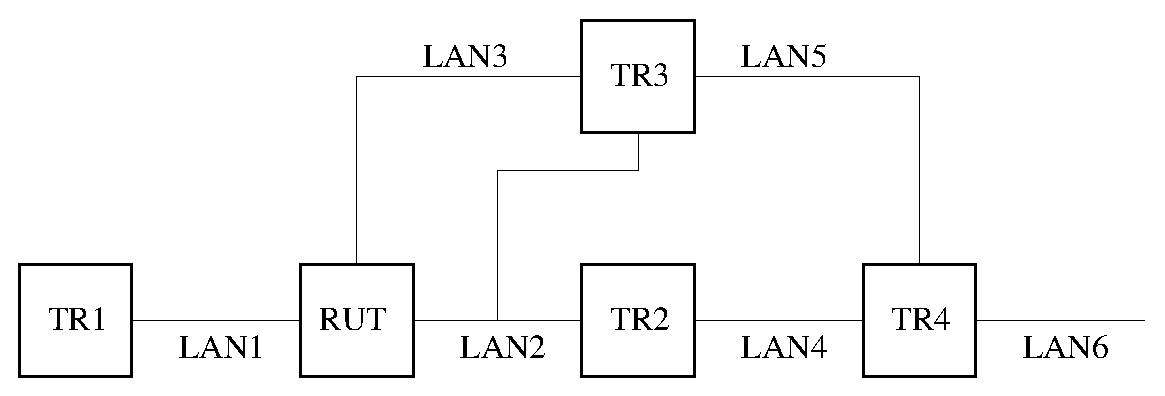
\includegraphics[scale=0.8]{figs/pim_test_6_1_candidate_bsr_state_machine}
    \caption{Candidate BSR state machine test setup}
    \label{fig:pim_test_6_1_candidate_bsr_state_machine}
  \end{center}
\end{figure}

\para{Procedure:}

\subpara{Part A: Receive preferred BSM in Pending BSR state.}

\begin{enumerate}

  \item Start the RUT and TR1, and start observing the Bootstrap messages
  transmitted on LAN1.

  \item Check the BSR status in the RUT.

  \item Compose a Bootstrap message at TR1 with the BSR address set to TR1,
  BSR priority of 10, Cand-RP set composed of TR1 as an RP for 226.0.0.0/8,
  and send it on LAN1.

  \item Right after the RUT receives the Bootstrap message, check the BSR
  status, and the RP-Set in the RUT.

\end{enumerate}

\subpara{Part B: BS Timer expires in Pending BSR state.}

\begin{enumerate}

  \item Configure the RUT as a Candidate-RP for 226.0.0.0/8.

  \item Start the RUT and TR1, and start observing the Bootstrap messages
  transmitted on LAN1.

  \item Check the BSR status in the RUT.

  \item Wait for up to \verb=BS_Timeout= ({\PimsmBSTimeout}) until the BS
  Timer in the RUT expires.

  \item After the BS Timer in the RUT expires, check the BSR status, and the
  RP-Set in the RUT.

\end{enumerate}

\subpara{Part C: Receive non-preferred BSM in Pending BSR state.}

The setup is same as in Part A, except that the BSR priority of the Bootstrap
message originated by TR1 is 0 instead of 10.

\subpara{Part D: Receive preferred BSM in Candidate BSR state.}

\begin{enumerate}

  \item Start the RUT, TR1, and TR2, and start observing the Bootstrap messages
  transmitted on LAN1 and LAN2.

  \item Check the BSR status in the RUT.

  \item Compose a Bootstrap message at TR1 with the BSR address set to TR1,
  BSR priority of 10, Cand-RP set composed of TR1 as an RP for 226.0.0.0/8,
  and send it on LAN1.

  \item Right after the RUT receives the Bootstrap message, check the BSR
  status, and the RP-Set in the RUT.

  \item Compose a Bootstrap message at TR2 with the BSR address set to TR2,
  BSR priority of 20, Cand-RP set composed of TR2 as an RP for 226.0.0.0/8,
  and send it on LAN2.

  \item Right after the RUT receives the Bootstrap message, check the BSR
  status, and the RP-Set in the RUT.

  \item Compose a Bootstrap message at TR2 with the BSR address set to TR2,
  BSR priority of 25, Cand-RP set composed of TR2 as an RP for 226.0.0.0/8,
  and send it on LAN2. However, the Fragment Tag for this message should be
  different from the Fragment Tag for the previous Bootstrap message.

  \item Right after the RUT receives the Bootstrap message, check the BSR
  status, and the RP-Set in the RUT.

\end{enumerate}

\subpara{Part E: BS Timer expires in Candidate BSR state.}

\begin{enumerate}

  \item Start the RUT and TR1, and start observing the Bootstrap messages
  transmitted on LAN1.

  \item Check the BSR status in the RUT.

  \item Compose a Bootstrap message at TR1 with the BSR address set to TR1,
  BSR priority of 10, Cand-RP set composed of TR1 as an RP for 226.0.0.0/8,
  and send it on LAN1.

  \item Right after the RUT receives the Bootstrap message, check the BSR
  status, and the RP-Set in the RUT.

  \item Wait for up to \verb=BS_Timeout= ({\PimsmBSTimeout}) until the BS
  Timer in the RUT expires.

  \item After the BS Timer in the RUT expires, check the BSR status, and the
  RP-Set in the RUT.

  \item Wait for up to \verb=rand_override= ({\PimsmRandOverride}) until the BS
  Timer in the RUT expires.

  \item After the BS Timer in the RUT expires, check the BSR status, and the
  RP-Set in the RUT.

\end{enumerate}

\subpara{Part F: Receive non-preferred BSM from elected BSR in Candidate BSR
state.}

\begin{enumerate}

  \item Start the RUT and TR1, and start observing the Bootstrap messages
  transmitted on LAN1.

  \item Check the BSR status in the RUT.

  \item Compose a Bootstrap message at TR1 with the BSR address set to TR1,
  BSR priority of 10, Cand-RP set composed of TR1 as an RP for 226.0.0.0/8,
  and send it on LAN1.

  \item Right after the RUT receives the Bootstrap message, check the BSR
  status, and the RP-Set in the RUT.

  \item Compose a Bootstrap message at TR1 with the BSR address set to TR1,
  BSR priority of 5, Cand-RP set composed of TR1 as an RP for 226.0.0.0/8,
  and send it on LAN1. However, the Fragment Tag for this message should be
  different from the Fragment Tag for the previous Bootstrap message.

  \item Right after the RUT receives the Bootstrap message, check the BSR
  status, and the RP-Set in the RUT.

  \item Wait for up to \verb=rand_override= ({\PimsmRandOverride}) until the BS
  Timer in the RUT expires.

  \item After the BS Timer in the RUT expires, check the BSR status, and the
  RP-Set in the RUT.

\end{enumerate}

\subpara{Part G: Receive preferred BSM in Elected BSR state.}

\begin{enumerate}

  \item Configure the RUT as a Candidate-RP for 226.0.0.0/8.

  \item Start the RUT and TR1, and start observing the Bootstrap messages
  transmitted on LAN1.

  \item Check the BSR status in the RUT.

  \item Wait for up to \verb=BS_Timeout= ({\PimsmBSTimeout}) until the BS
  Timer in the RUT expires.

  \item After the BS Timer in the RUT expires, check the BSR status, and the
  RP-Set in the RUT.

  \item Compose a Bootstrap message at TR1 with the BSR address set to TR1,
  BSR priority of 10, Cand-RP set composed of TR1 as an RP for 226.0.0.0/8,
  and send it on LAN1.

  \item Right after the RUT receives the Bootstrap message, check the BSR
  status, and the RP-Set in the RUT.

\end{enumerate}

\subpara{Part H: BS Timer expires in Elected BSR state.}

\begin{enumerate}

  \item Configure the RUT as a Candidate-RP for 226.0.0.0/8.

  \item Start the RUT and TR1, and start observing the Bootstrap messages
  transmitted on LAN1.

  \item Check the BSR status in the RUT.

  \item Wait for up to \verb=BS_Timeout= ({\PimsmBSTimeout}) until the BS
  Timer in the RUT expires.

  \item After the BS Timer in the RUT expires, check the BSR status, and the
  RP-Set in the RUT.

  \item Wait for up to \verb=BS_Period= ({\PimsmBSPeriod}) until the BS
  Timer in the RUT expires.

  \item After the BS Timer in the RUT expires, check the BSR status, and the
  RP-Set in the RUT.

\end{enumerate}

\subpara{Part I: Receive non-preferred BSM in Elected BSR state.}

The setup is same as in Part G, except that the BSR priority of the Bootstrap
message originated by TR1 is 0 instead of 10.

\para{Observable Results:}

\subpara{Part A:}

\begin{itemize}

  \item Right after the RUT is started, its BSR state machine should be in
  Pending state:

\begin{verbatim}
Xorp> show pim bootstrap 
Active zones:
BSR              Pri LocalAddress     Pri State            Timeout SZTimeout
0.0.0.0            0 10.2.0.1           1 Pending               84        -1
Expiring zones:
BSR              Pri LocalAddress     Pri State            Timeout SZTimeout
Configured zones:
BSR              Pri LocalAddress     Pri State            Timeout SZTimeout
10.2.0.1           1 10.2.0.1           1 Init                  -1        -1
\end{verbatim}

  \item After the RUT receives the Bootstrap message, it should forward it
        back on LAN1. Its BSR state machine
        should be in Candidate BSR state, and the elected BSR should be TR1.
        The BS Timer in the RUT should be set to \verb=BS_Timeout=
        ({\PimsmBSTimeout}):

\begin{verbatim}
Xorp> show pim bootstrap 
Active zones:
BSR              Pri LocalAddress     Pri State            Timeout SZTimeout
10.6.0.1          10 10.2.0.1           1 Candidate            127        -1
Expiring zones:
BSR              Pri LocalAddress     Pri State            Timeout SZTimeout
Configured zones:
BSR              Pri LocalAddress     Pri State            Timeout SZTimeout
10.2.0.1           1 10.2.0.1           1 Init                  -1        -1
\end{verbatim}

  In addition, the RP-Set should contain TR1 as the RP for 226.0.0.0/8:

\begin{verbatim}
Xorp> show pim bootstrap rps 
Active RPs:
RP               Pri Timeout GroupPrefix        BSR         CandRpAdvTimeout
10.6.0.1         192     145 226.0.0.0/8        10.6.0.1                  -1
Expiring RPs:
RP               Pri Timeout GroupPrefix        BSR         CandRpAdvTimeout
Configured RPs:
RP               Pri Timeout GroupPrefix        BSR         CandRpAdvTimeout
\end{verbatim}

\end{itemize}

\subpara{Part B:}

\begin{itemize}

  \item Right after the RUT is started, its BSR state machine should be in
  Pending state:

\begin{verbatim}
Xorp> show pim bootstrap 
Active zones:
BSR              Pri LocalAddress     Pri State            Timeout SZTimeout
0.0.0.0            0 10.2.0.1           1 Pending               83        -1
Expiring zones:
BSR              Pri LocalAddress     Pri State            Timeout SZTimeout
Configured zones:
BSR              Pri LocalAddress     Pri State            Timeout SZTimeout
10.2.0.1           1 10.2.0.1           1 Init                  -1        -1
\end{verbatim}

  \item After the BS Timer in the RUT expires, the RUT should store itself in
        the RP-Set, and should originate a Bootstrap message on LAN1.
        Its BSR state machine should be in Elected BSR state, and the elected
        BSR should be the RUT.
        The BS Timer in the RUT should be set to \verb=BS_Period=
        ({\PimsmBSPeriod}):

\begin{verbatim}
Xorp> show pim bootstrap 
Active zones:
BSR              Pri LocalAddress     Pri State            Timeout SZTimeout
10.2.0.1           1 10.2.0.1           1 Elected               58        -1
Expiring zones:
BSR              Pri LocalAddress     Pri State            Timeout SZTimeout
Configured zones:
BSR              Pri LocalAddress     Pri State            Timeout SZTimeout
10.2.0.1           1 10.2.0.1           1 Init                  -1        -1
\end{verbatim}

  In addition, the RP-Set should contain the RUT as the RP for 226.0.0.0/8:

\begin{verbatim}
Xorp> show pim bootstrap rps 
Active RPs:
RP               Pri Timeout GroupPrefix        BSR         CandRpAdvTimeout
10.2.0.1         192      -1 226.0.0.0/8        10.2.0.1                  -1
Expiring RPs:
RP               Pri Timeout GroupPrefix        BSR         CandRpAdvTimeout
Configured RPs:
RP               Pri Timeout GroupPrefix        BSR         CandRpAdvTimeout
10.2.0.1         192      -1 226.0.0.0/8        10.2.0.1                  42
\end{verbatim}

\end{itemize}

\subpara{Part C:}

\begin{itemize}

  \item Right after the RUT is started, its BSR state machine should be in
  Pending state:

\begin{verbatim}
Xorp> show pim bootstrap 
Active zones:
BSR              Pri LocalAddress     Pri State            Timeout SZTimeout
0.0.0.0            0 10.2.0.1           1 Pending               85        -1
Expiring zones:
BSR              Pri LocalAddress     Pri State            Timeout SZTimeout
Configured zones:
BSR              Pri LocalAddress     Pri State            Timeout SZTimeout
10.2.0.1           1 10.2.0.1           1 Init                  -1        -1
\end{verbatim}

  \item After the RUT receives the Bootstrap message, it should silently
        ignore it.
        Its BSR state machine should continue to be in Pending BSR state:

\begin{verbatim}
Xorp> show pim bootstrap 
Active zones:
BSR              Pri LocalAddress     Pri State            Timeout SZTimeout
0.0.0.0            0 10.2.0.1           1 Pending               71        -1
Expiring zones:
BSR              Pri LocalAddress     Pri State            Timeout SZTimeout
Configured zones:
BSR              Pri LocalAddress     Pri State            Timeout SZTimeout
10.2.0.1           1 10.2.0.1           1 Init                  -1        -1
\end{verbatim}

  In addition, the RP-Set not be modified:

\begin{verbatim}
Xorp> show pim bootstrap rps 
Active RPs:
RP               Pri Timeout GroupPrefix        BSR         CandRpAdvTimeout
Expiring RPs:
RP               Pri Timeout GroupPrefix        BSR         CandRpAdvTimeout
Configured RPs:
RP               Pri Timeout GroupPrefix        BSR         CandRpAdvTimeout
\end{verbatim}

\end{itemize}

\subpara{Part D:}

\begin{itemize}

  \item Right after the RUT is started, its BSR state machine should be in
  Pending state:

\begin{verbatim}
Xorp> show pim bootstrap 
Active zones:
BSR              Pri LocalAddress     Pri State            Timeout SZTimeout
0.0.0.0            0 10.2.0.1           1 Pending              152        -1
Expiring zones:
BSR              Pri LocalAddress     Pri State            Timeout SZTimeout
Configured zones:
BSR              Pri LocalAddress     Pri State            Timeout SZTimeout
10.2.0.1           1 10.2.0.1           1 Init                  -1        -1
\end{verbatim}

  \item After the RUT receives the first Bootstrap message, it should forward
        it on LAN2, and back on LAN1. Its BSR state machine
        should be in Candidate BSR state, and the elected BSR should be TR1.
        The BS Timer in the RUT should be set to \verb=BS_Timeout=
        ({\PimsmBSTimeout}):

\begin{verbatim}
Xorp> show pim bootstrap 
Active zones:
BSR              Pri LocalAddress     Pri State            Timeout SZTimeout
10.6.0.1          10 10.2.0.1           1 Candidate            128        -1
Expiring zones:
BSR              Pri LocalAddress     Pri State            Timeout SZTimeout
Configured zones:
BSR              Pri LocalAddress     Pri State            Timeout SZTimeout
10.2.0.1           1 10.2.0.1           1 Init                  -1        -1
\end{verbatim}

  In addition, the RP-Set should contain TR1 as the RP for 226.0.0.0/8:

\begin{verbatim}
Xorp> show pim bootstrap rps 
Active RPs:
RP               Pri Timeout GroupPrefix        BSR         CandRpAdvTimeout
10.6.0.1         192     144 226.0.0.0/8        10.6.0.1                  -1
Expiring RPs:
RP               Pri Timeout GroupPrefix        BSR         CandRpAdvTimeout
Configured RPs:
RP               Pri Timeout GroupPrefix        BSR         CandRpAdvTimeout
\end{verbatim}

  \item After the RUT receives the second Bootstrap message, it should forward
        it on LAN1, and back on LAN2. Its BSR state machine
        should continue be in Candidate BSR state, but the elected BSR should
        be TR2.
        The BS Timer in the RUT should be set to \verb=BS_Timeout=
        ({\PimsmBSTimeout}):

\begin{verbatim}
Xorp> show pim bootstrap 
Active zones:
BSR              Pri LocalAddress     Pri State            Timeout SZTimeout
10.3.0.1          20 10.2.0.1           1 Candidate            128        -1
Expiring zones:
BSR              Pri LocalAddress     Pri State            Timeout SZTimeout
Configured zones:
BSR              Pri LocalAddress     Pri State            Timeout SZTimeout
10.2.0.1           1 10.2.0.1           1 Init                  -1        -1
\end{verbatim}

  In addition, the RP-Set should contain TR2 as the RP for 226.0.0.0/8:

\begin{verbatim}
Xorp> show pim bootstrap rps 
Active RPs:
RP               Pri Timeout GroupPrefix        BSR         CandRpAdvTimeout
10.3.0.1         192     145 226.0.0.0/8        10.3.0.1                  -1
Expiring RPs:
RP               Pri Timeout GroupPrefix        BSR         CandRpAdvTimeout
Configured RPs:
RP               Pri Timeout GroupPrefix        BSR         CandRpAdvTimeout
\end{verbatim}

  \item After the RUT receives the third Bootstrap message, it should forward
        it on LAN1, and back on LAN2. Its BSR state machine
        should continue be in Candidate BSR state, and the elected BSR should
        continue be TR2.
        The BS Timer in the RUT should be set to \verb=BS_Timeout=
        ({\PimsmBSTimeout}). However, the BSR priority should be updated to 25:

\begin{verbatim}
Xorp> show pim bootstrap 
Active zones:
BSR              Pri LocalAddress     Pri State            Timeout SZTimeout
10.3.0.1          25 10.2.0.1           1 Candidate            128        -1
Expiring zones:
BSR              Pri LocalAddress     Pri State            Timeout SZTimeout
Configured zones:
BSR              Pri LocalAddress     Pri State            Timeout SZTimeout
10.2.0.1           1 10.2.0.1           1 Init                  -1        -1
\end{verbatim}

  In addition, the RP-Set should continue to contain TR2 as the RP for
  226.0.0.0/8:

\begin{verbatim}
Xorp> show pim bootstrap rps 
Active RPs:
RP               Pri Timeout GroupPrefix        BSR         CandRpAdvTimeout
10.3.0.1         192     143 226.0.0.0/8        10.3.0.1                  -1
Expiring RPs:
RP               Pri Timeout GroupPrefix        BSR         CandRpAdvTimeout
Configured RPs:
RP               Pri Timeout GroupPrefix        BSR         CandRpAdvTimeout
\end{verbatim}

\end{itemize}

\subpara{Part E:}

\begin{itemize}

  \item Right after the RUT is started, its BSR state machine should be in
  Pending state:

\begin{verbatim}
Xorp> show pim bootstrap 
Active zones:
BSR              Pri LocalAddress     Pri State            Timeout SZTimeout
0.0.0.0            0 10.2.0.1           1 Pending               98        -1
Expiring zones:
BSR              Pri LocalAddress     Pri State            Timeout SZTimeout
Configured zones:
BSR              Pri LocalAddress     Pri State            Timeout SZTimeout
10.2.0.1           1 10.2.0.1           1 Init                  -1        -1
\end{verbatim}

  \item After the RUT receives the first Bootstrap message, it should forward
        it on LAN2, and back on LAN1. Its BSR state machine
        should be in Candidate BSR state, and the elected BSR should be TR1.
        The BS Timer in the RUT should be set to \verb=BS_Timeout=
        ({\PimsmBSTimeout}):

\begin{verbatim}
Xorp> show pim bootstrap 
Active zones:
BSR              Pri LocalAddress     Pri State            Timeout SZTimeout
10.6.0.1          10 10.2.0.1           1 Candidate            127        -1
Expiring zones:
BSR              Pri LocalAddress     Pri State            Timeout SZTimeout
Configured zones:
BSR              Pri LocalAddress     Pri State            Timeout SZTimeout
10.2.0.1           1 10.2.0.1           1 Init                  -1        -1
\end{verbatim}

  In addition, the RP-Set should contain TR1 as the RP for 226.0.0.0/8:

\begin{verbatim}
Xorp> show pim bootstrap rps 
Active RPs:
RP               Pri Timeout GroupPrefix        BSR         CandRpAdvTimeout
10.6.0.1         192     145 226.0.0.0/8        10.6.0.1                  -1
Expiring RPs:
RP               Pri Timeout GroupPrefix        BSR         CandRpAdvTimeout
Configured RPs:
RP               Pri Timeout GroupPrefix        BSR         CandRpAdvTimeout
\end{verbatim}

  \item After up to \verb=BS_Timeout= ({\PimsmBSTimeout}) the BS Timer in the
  RUT should expire.

  \item After the BS Timer in the RUT expires, the BSR state machine should be
  in Pending BSR, and the BS Timer should be set to \verb=rand_override=
  ({\PimsmRandOverride}):

\begin{verbatim}
Xorp> show pim bootstrap 
Active zones:
BSR              Pri LocalAddress     Pri State            Timeout SZTimeout
10.6.0.1          10 10.2.0.1           1 Pending               13        -1
Expiring zones:
BSR              Pri LocalAddress     Pri State            Timeout SZTimeout
Configured zones:
BSR              Pri LocalAddress     Pri State            Timeout SZTimeout
10.2.0.1           1 10.2.0.1           1 Init                  -1        -1
\end{verbatim}

  In addition, the RP-Set should still contain TR1 as the RP for 226.0.0.0/8:

\begin{verbatim}
Xorp> show pim bootstrap rps 
Active RPs:
RP               Pri Timeout GroupPrefix        BSR         CandRpAdvTimeout
10.6.0.1         192      17 226.0.0.0/8        10.6.0.1                  -1
Expiring RPs:
RP               Pri Timeout GroupPrefix        BSR         CandRpAdvTimeout
Configured RPs:
RP               Pri Timeout GroupPrefix        BSR         CandRpAdvTimeout
\end{verbatim}

  \item After up to \verb=rand_override= ({\PimsmRandOverride}) the BS Timer
  in the RUT should expire.

  \item After the BS Timer in the RUT expires, the BSR state machine should be
  in Elected BSR state, the RUT should originate a Bootstrap message on LAN1,
  and the elected BSR should be the RUT itself.
  The BS Timer in the RUT should be set to \verb=BS_Period=
  ({\PimsmBSPeriod}):

\begin{verbatim}
Xorp> show pim bootstrap 
Active zones:
BSR              Pri LocalAddress     Pri State            Timeout SZTimeout
10.2.0.1           1 10.2.0.1           1 Elected               57        -1
Expiring zones:
BSR              Pri LocalAddress     Pri State            Timeout SZTimeout
10.6.0.1          10 10.2.0.1           1 Elected                0        -1
Configured zones:
BSR              Pri LocalAddress     Pri State            Timeout SZTimeout
10.2.0.1           1 10.2.0.1           1 Init                  -1        -1
\end{verbatim}

  In addition, the RP-Set should still contain TR1 as the RP for 226.0.0.0/8:

\begin{verbatim}
Xorp> show pim bootstrap rps 
Active RPs:
RP               Pri Timeout GroupPrefix        BSR         CandRpAdvTimeout
Expiring RPs:
RP               Pri Timeout GroupPrefix        BSR         CandRpAdvTimeout
10.6.0.1         192       2 226.0.0.0/8        10.6.0.1                  -1
Configured RPs:
RP               Pri Timeout GroupPrefix        BSR         CandRpAdvTimeout
\end{verbatim}

\end{itemize}

\subpara{Part F:}

The results should be same as in Part E, except that the transition
of the BSR state machine of the RUT from Candidate BSR state to
Pending BSR state should be triggered by the second Bootstrap message
originated by TR1.

\subpara{Part G:}

\begin{itemize}

  \item Right after the RUT is started, its BSR state machine should be in
  Pending state:

\begin{verbatim}
Xorp> show pim bootstrap 
Active zones:
BSR              Pri LocalAddress     Pri State            Timeout SZTimeout
0.0.0.0            0 10.2.0.1           1 Pending              160        -1
Expiring zones:
BSR              Pri LocalAddress     Pri State            Timeout SZTimeout
Configured zones:
BSR              Pri LocalAddress     Pri State            Timeout SZTimeout
10.2.0.1           1 10.2.0.1           1 Init                  -1        -1
\end{verbatim}

  \item After up to \verb=BS_Timeout= ({\PimsmBSTimeout}) the BS Timer
  in the RUT should expire.

  \item After the BS Timer in the RUT expires, the BSR state machine should be
  in Elected BSR state, the RUT should originate a Bootstrap message on LAN1,
  and the elected BSR should be the RUT itself.
  The BS Timer in the RUT should be set to \verb=BS_Period=
  ({\PimsmBSPeriod}):

\begin{verbatim}
Xorp> show pim bootstrap 
Active zones:
BSR              Pri LocalAddress     Pri State            Timeout SZTimeout
10.2.0.1           1 10.2.0.1           1 Elected               57        -1
Expiring zones:
BSR              Pri LocalAddress     Pri State            Timeout SZTimeout
Configured zones:
BSR              Pri LocalAddress     Pri State            Timeout SZTimeout
10.2.0.1           1 10.2.0.1           1 Init                  -1        -1
\end{verbatim}

  In addition, the RP-Set should contain the RUT as the RP for 226.0.0.0/8:

\begin{verbatim}
Xorp> show pim bootstrap rps 
Active RPs:
RP               Pri Timeout GroupPrefix        BSR         CandRpAdvTimeout
10.2.0.1         192      -1 226.0.0.0/8        10.2.0.1                  -1
Expiring RPs:
RP               Pri Timeout GroupPrefix        BSR         CandRpAdvTimeout
Configured RPs:
RP               Pri Timeout GroupPrefix        BSR         CandRpAdvTimeout
10.2.0.1         192      -1 226.0.0.0/8        10.2.0.1                  20
\end{verbatim}

  \item After the RUT receives the Bootstrap message, it should forward
        it on LAN1. Its BSR state machine
        should be in Candidate BSR state, and the elected BSR should be TR1.
        The BS Timer in the RUT should be set to \verb=BS_Timeout=
        ({\PimsmBSTimeout}):

\begin{verbatim}
Xorp> show pim bootstrap 
Active zones:
BSR              Pri LocalAddress     Pri State            Timeout SZTimeout
10.6.0.1          10 10.2.0.1           1 Candidate            126        -1
Expiring zones:
BSR              Pri LocalAddress     Pri State            Timeout SZTimeout
Configured zones:
BSR              Pri LocalAddress     Pri State            Timeout SZTimeout
10.2.0.1           1 10.2.0.1           1 Init                  -1        -1
\end{verbatim}

  In addition, the RP-Set should contain TR1 as the RP for 226.0.0.0/8:

\begin{verbatim}
Xorp> show pim bootstrap rps 
Active RPs:
RP               Pri Timeout GroupPrefix        BSR         CandRpAdvTimeout
10.6.0.1         192     142 226.0.0.0/8        10.6.0.1                  -1
Expiring RPs:
RP               Pri Timeout GroupPrefix        BSR         CandRpAdvTimeout
Configured RPs:
RP               Pri Timeout GroupPrefix        BSR         CandRpAdvTimeout
10.2.0.1         192      -1 226.0.0.0/8        10.2.0.1                  52
\end{verbatim}

\end{itemize}

\subpara{Part H:}

\begin{itemize}

  \item Right after the RUT is started, its BSR state machine should be in
  Pending state:

\begin{verbatim}
Xorp> show pim bootstrap 
Active zones:
BSR              Pri LocalAddress     Pri State            Timeout SZTimeout
0.0.0.0            0 10.2.0.1           1 Pending               88        -1
Expiring zones:
BSR              Pri LocalAddress     Pri State            Timeout SZTimeout
Configured zones:
BSR              Pri LocalAddress     Pri State            Timeout SZTimeout
10.2.0.1           1 10.2.0.1           1 Init                  -1        -1
\end{verbatim}

  \item After up to \verb=BS_Timeout= ({\PimsmBSTimeout}) the BS Timer
  in the RUT should expire.

  \item After the BS Timer in the RUT expires, the BSR state machine should be
  in Elected BSR state, the RUT should originate a Bootstrap message on LAN1,
  and the elected BSR should be the RUT itself.
  The BS Timer in the RUT should be set to \verb=BS_Period=
  ({\PimsmBSPeriod}):

\begin{verbatim}
Xorp> show pim bootstrap 
Active zones:
BSR              Pri LocalAddress     Pri State            Timeout SZTimeout
10.2.0.1           1 10.2.0.1           1 Elected               58        -1
Expiring zones:
BSR              Pri LocalAddress     Pri State            Timeout SZTimeout
Configured zones:
BSR              Pri LocalAddress     Pri State            Timeout SZTimeout
10.2.0.1           1 10.2.0.1           1 Init                  -1        -1
\end{verbatim}

  In addition, the RP-Set should contain the RUT as the RP for 226.0.0.0/8:

\begin{verbatim}
Xorp> show pim bootstrap rps 
Active RPs:
RP               Pri Timeout GroupPrefix        BSR         CandRpAdvTimeout
10.2.0.1         192      -1 226.0.0.0/8        10.2.0.1                  -1
Expiring RPs:
RP               Pri Timeout GroupPrefix        BSR         CandRpAdvTimeout
Configured RPs:
RP               Pri Timeout GroupPrefix        BSR         CandRpAdvTimeout
10.2.0.1         192      -1 226.0.0.0/8        10.2.0.1                  24
\end{verbatim}

  \item After \verb=BS_Period= ({\PimsmBSPeriod}) the BS Timer
  in the RUT should expire.

  \item After the BS Timer in the RUT expires, the BSR state machine should
  continue to be in Elected BSR state, the RUT should originate a Bootstrap
  message on LAN1, and the elected BSR should be the RUT itself.
  The BS Timer in the RUT should be set to \verb=BS_Period=
  ({\PimsmBSPeriod}):

\begin{verbatim}
Xorp> show pim bootstrap 
Active zones:
BSR              Pri LocalAddress     Pri State            Timeout SZTimeout
10.2.0.1           1 10.2.0.1           1 Elected               55        -1
Expiring zones:
BSR              Pri LocalAddress     Pri State            Timeout SZTimeout
Configured zones:
BSR              Pri LocalAddress     Pri State            Timeout SZTimeout
10.2.0.1           1 10.2.0.1           1 Init                  -1        -1
\end{verbatim}

  In addition, the RP-Set should continue to contain the RUT as the RP for
  226.0.0.0/8:

\begin{verbatim}
Xorp> show pim bootstrap rps 
Active RPs:
RP               Pri Timeout GroupPrefix        BSR         CandRpAdvTimeout
10.2.0.1         192      -1 226.0.0.0/8        10.2.0.1                  -1
Expiring RPs:
RP               Pri Timeout GroupPrefix        BSR         CandRpAdvTimeout
Configured RPs:
RP               Pri Timeout GroupPrefix        BSR         CandRpAdvTimeout
10.2.0.1         192      -1 226.0.0.0/8        10.2.0.1                  25
\end{verbatim}

\end{itemize}

\subpara{Part I:}

The results should be same as in Part H, except that the same actions that
were triggered when the RUT is in Elected BSR state and the BS Timer expired,
in this part those actions should be triggered when the RUT receives the
Bootstrap message originated by TR1.

\para{Possible Problems:}
The RUT might become the BSR earlier or later than \verb=BS_Timeout=
({\PimsmBSTimeout}) if the implementation uses shorter or longer timeout
interval on startup (\eg if it has tuned for fast start-up, or if it uses a
randomized timeout interval).
In Part E, if the Cand-RP holdtime of TR1 is too short, TR1 may expire from
the RP-Set before the BSR state machine of RUT transitions to Pending BSR or
Elected BSR state.


%%%%%%%%%%%%%%%%%%%%%%%%%%%%%%%%%%%%%%%%%%%
\newpage
\section{Non-Candidate BSR State Machine}

\para{Purpose:}
Test the per-scope-zone state machine for a non-candidate BSR.

\para{References:}
\begin{itemize}
  \item draft-ietf-pim-sm-bsr-03 -- Section 3
\end{itemize}

\para{Discussion:}
Non-candidate BSRs listen for Bootstrap messages which contain information
such as BSR-priority and BSR-address of the candidate BSRs.
This information is used
to elect a single BSR per scope-zone per domain. The elected BSR then
periodically originates a Bootstrap message that contains also the
candidate-RP information. The candidate-RP information is used to compose the
RP-Set in all PIM-SM routers within the same domain. If a non-candidate BSR has
not received the Bootstrap message from the elected BSR for some amount of
time, then the elected BSR is timed-out.

\para{Test Setup:}
Connect the RUT, TR1, TR2, TR3, and TR4 according to
Figure~\ref{fig:pim_test_6_2_non_candidate_bsr_state_machine}.
Enable PIM-SM on the RUT, TR1, TR2, TR3, and TR4. Do NOT configure the RUT as
a Cand-BSR.

\begin{figure}[htbp]
  \begin{center}
    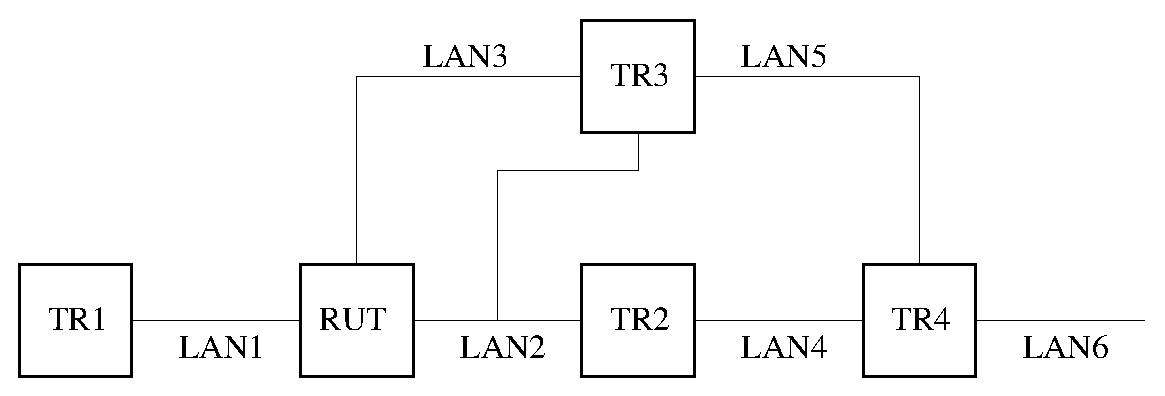
\includegraphics[scale=0.8]{figs/pim_test_6_2_non_candidate_bsr_state_machine}
    \caption{Non-candidate BSR state machine test setup}
    \label{fig:pim_test_6_2_non_candidate_bsr_state_machine}
  \end{center}
\end{figure}

\para{Procedure:}

\subpara{Part A: Receive BSM for unknown Admin Scope in No Info state.}

\begin{enumerate}

  \item Start the RUT and TR1, and start observing the Bootstrap messages
  transmitted on LAN1.

  \item Check the BSR status in the RUT.

  \item Compose a Bootstrap message at TR1 with the BSR address set to TR1,
  BSR priority of 10, Cand-RP set composed of TR1 as an RP for 226.0.0.0/8,
  and send it on LAN1.

  \item Right after the RUT receives the Bootstrap message, check the BSR
  status, and the RP-Set in the RUT.

\end{enumerate}

\subpara{Part B: Receive preferred BSM in Accept Preferred state.}

\begin{enumerate}

  \item Start the RUT, TR1, and TR2, and start observing the Bootstrap messages
  transmitted on LAN1.

  \item Check the BSR status in the RUT.

  \item Compose a Bootstrap message at TR1 with the BSR address set to TR1,
  BSR priority of 10, Cand-RP set composed of TR1 as an RP for 226.0.0.0/8,
  and send it on LAN1.

  \item Right after the RUT receives the Bootstrap message, check the BSR
  status, and the RP-Set in the RUT.

  \item Compose a Bootstrap message at TR2 with the BSR address set to TR2,
  BSR priority of 20, Cand-RP set composed of TR2 as an RP for 226.0.0.0/8,
  and send it on LAN2.

  \item Right after the RUT receives the Bootstrap message, check the BSR
  status, and the RP-Set in the RUT.

\end{enumerate}

\subpara{Part C: BS Timer expires in Accept Preferred state.}

\begin{enumerate}

  \item Start the RUT and TR1, and start observing the Bootstrap messages
  transmitted on LAN1.

  \item Check the BSR status in the RUT.

  \item Compose a Bootstrap message at TR1 with the BSR address set to TR1,
  BSR priority of 10, Cand-RP set composed of TR1 as an RP for 226.0.0.0/8,
  and send it on LAN1.

  \item Right after the RUT receives the Bootstrap message, check the BSR
  status, and the RP-Set in the RUT.

  \item Wait for up to \verb=BS_Timeout= ({\PimsmBSTimeout}) until the BS
  Timer in the RUT expires.

  \item After the BS Timer in the RUT expires, check the BSR status, and the
  RP-Set in the RUT.

\end{enumerate}

\subpara{Part D: Receive non-preferred BSM in Accept Preferred state.}

The setup is same as in Part B, except that the BSR priority of the Bootstrap
message originated by TR2 is 0 instead of 20.

\subpara{Part E: Receive BSM in Accept Any state.}

\begin{enumerate}

  \item Start the RUT, TR1, and TR2, and start observing the Bootstrap messages
  transmitted on LAN1 and LAN2.

  \item Check the BSR status in the RUT.

  \item Compose a Bootstrap message at TR1 with the BSR address set to TR1,
  BSR priority of 10, Cand-RP set composed of TR1 as an RP for 226.0.0.0/8,
  and send it on LAN1.

  \item Right after the RUT receives the Bootstrap message, check the BSR
  status, and the RP-Set in the RUT.

  \item Wait for up to \verb=BS_Timeout= ({\PimsmBSTimeout}) until the BS
  Timer in the RUT expires.

  \item After the BS Timer in the RUT expires, check the BSR status, and the
  RP-Set in the RUT.

  \item Compose a Bootstrap message at TR2 with the BSR address set to TR2,
  BSR priority of 0, Cand-RP set composed of TR2 as an RP for 226.0.0.0/8,
  and send it on LAN2.

  \item Right after the RUT receives the Bootstrap message, check the BSR
  status, and the RP-Set in the RUT.

\end{enumerate}

\subpara{Part F: SZ Timer expires in Accept Any.}

\begin{enumerate}

  \item Start the RUT and TR1, and start observing the Bootstrap messages
  transmitted on LAN1.

  \item Check the BSR status in the RUT.

  \item Compose a Bootstrap message at TR1 with the BSR address set to TR1,
  BSR priority of 10, Cand-RP set composed of TR1 as an RP for 226.0.0.0/8,
  and send it on LAN1.

  \item Right after the RUT receives the Bootstrap message, check the BSR
  status, and the RP-Set in the RUT.

  \item Wait for up to \verb=BS_Timeout= ({\PimsmBSTimeout}) until the BS
  Timer in the RUT expires.

  \item After the BS Timer in the RUT expires, check the BSR status, and the
  RP-Set in the RUT.

  \item Wait for up to \verb=SZ_Timeout= ({\PimsmSZTimeout}) until the BS
  Timer in the RUT expires.

  \item After the BS Timer in the RUT expires, check the BSR status, and the
  RP-Set in the RUT.

\end{enumerate}

\para{Observable Results:}

\subpara{Part A:}

\begin{itemize}

  \item Right after the RUT is started, its BSR state machine should be in
  No Info state:

\begin{verbatim}
Xorp> show pim bootstrap 
Active zones:
BSR              Pri LocalAddress     Pri State            Timeout SZTimeout
Expiring zones:
BSR              Pri LocalAddress     Pri State            Timeout SZTimeout
Configured zones:
BSR              Pri LocalAddress     Pri State            Timeout SZTimeout
0.0.0.0            0 0.0.0.0            0 Init                  -1        -1
\end{verbatim}

  \item After the RUT receives the Bootstrap message, it should forward it
        back on LAN1. Its BSR state machine
        should be in Accept Preferred state, and the elected BSR should be TR1.
        The BS Timer in the RUT should be set to \verb=BS_Timeout=
        ({\PimsmBSTimeout}).
        The SZ Timer in the RUT should be set to \verb=SZ_Timeout=
        ({\PimsmSZTimeout}):

\begin{verbatim}
Xorp> show pim bootstrap 
Active zones:
BSR              Pri LocalAddress     Pri State            Timeout SZTimeout
10.6.0.1          10 0.0.0.0            0 AcceptPreferred      127      1297
Expiring zones:
BSR              Pri LocalAddress     Pri State            Timeout SZTimeout
Configured zones:
BSR              Pri LocalAddress     Pri State            Timeout SZTimeout
0.0.0.0            0 0.0.0.0            0 Init                  -1        -1
\end{verbatim}

  In addition, the RP-Set should contain TR1 as the RP for 226.0.0.0/8:

\begin{verbatim}
Xorp> show pim bootstrap rps 
Active RPs:
RP               Pri Timeout GroupPrefix        BSR         CandRpAdvTimeout
10.6.0.1         192     145 226.0.0.0/8        10.6.0.1                  -1
Expiring RPs:
RP               Pri Timeout GroupPrefix        BSR         CandRpAdvTimeout
Configured RPs:
RP               Pri Timeout GroupPrefix        BSR         CandRpAdvTimeout
10.2.0.1         192      -1 226.0.0.0/8        0.0.0.0                   55
\end{verbatim}

\end{itemize}

\subpara{Part B:}

\begin{itemize}

  \item The results until after the first Bootstrap message is received should
  be same as in Part A, except that the Bootstrap message is forwarded on LAN2
  as well.

  \item After the RUT receives the second Bootstrap message, it should forward
        it on LAN1, and back on LAN2. Its BSR state machine
        should be in Accept Preferred state, and the elected BSR should be TR2.
        The BS Timer in the RUT should be set to \verb=BS_Timeout=
        ({\PimsmBSTimeout}).
        The SZ Timer in the RUT should be set to \verb=SZ_Timeout=
        ({\PimsmSZTimeout}):

\begin{verbatim}
Xorp> show pim bootstrap 
Active zones:
BSR              Pri LocalAddress     Pri State            Timeout SZTimeout
10.3.0.1          20 0.0.0.0            0 AcceptPreferred      125      1295
Expiring zones:
BSR              Pri LocalAddress     Pri State            Timeout SZTimeout
Configured zones:
BSR              Pri LocalAddress     Pri State            Timeout SZTimeout
0.0.0.0            0 0.0.0.0            0 Init                  -1        -1
\end{verbatim}

  In addition, the RP-Set should contain TR2 as the RP for 226.0.0.0/8:

\begin{verbatim}
Xorp> show pim bootstrap rps 
Active RPs:
RP               Pri Timeout GroupPrefix        BSR         CandRpAdvTimeout
10.3.0.1         192     141 226.0.0.0/8        10.3.0.1                  -1
Expiring RPs:
RP               Pri Timeout GroupPrefix        BSR         CandRpAdvTimeout
Configured RPs:
RP               Pri Timeout GroupPrefix        BSR         CandRpAdvTimeout
10.2.0.1         192      -1 226.0.0.0/8        0.0.0.0                   51
\end{verbatim}

\end{itemize}

\subpara{Part C:}

\begin{itemize}

  \item The results until after the first Bootstrap message is received should
  be same as in Part A.

  \item After the BS Timer in the RUT expires, the BSR state machine should be
  in Accept Any state:

\begin{verbatim}
Xorp> show pim bootstrap
Active zones:
BSR              Pri LocalAddress     Pri State            Timeout SZTimeout
10.6.0.1          10 0.0.0.0            0 AcceptAny              0      1167
Expiring zones:
BSR              Pri LocalAddress     Pri State            Timeout SZTimeout
Configured zones:
BSR              Pri LocalAddress     Pri State            Timeout SZTimeout
0.0.0.0            0 0.0.0.0            0 Init                  -1        -1
\end{verbatim}

  In addition, the RP-Set not be modified:

\begin{verbatim}
Xorp> show pim bootstrap rps 
Active RPs:
RP               Pri Timeout GroupPrefix        BSR         CandRpAdvTimeout
10.6.0.1         192      16 226.0.0.0/8        10.6.0.1                  -1
Expiring RPs:
RP               Pri Timeout GroupPrefix        BSR         CandRpAdvTimeout
Configured RPs:
RP               Pri Timeout GroupPrefix        BSR         CandRpAdvTimeout
10.2.0.1         192      -1 226.0.0.0/8        0.0.0.0                   46
\end{verbatim}

\end{itemize}

\subpara{Part D:}

\begin{itemize}

  \item The results until after the first Bootstrap message is received should
  be same as in Part A.

  \item After the second Bootstrap message is received, the BSR state and the
  Cand-RP set in the RUT should not be modified.

\end{itemize}

\subpara{Part E:}

\begin{itemize}

  \item The results until after the BS Timer expires should be same as in Part
  C, except that the Bootstrap message is forwarded on LAN2 as well.

  \item After the RUT receives the second Bootstrap message, it should forward
        it on LAN1, and back on LAN2. Its BSR state machine
        should be in Accept Preferred state, and the elected BSR should be TR2.
        The BS Timer in the RUT should be set to \verb=BS_Timeout=
        ({\PimsmBSTimeout}).
        The SZ Timer in the RUT should be set to \verb=SZ_Timeout=
        ({\PimsmSZTimeout}):

\begin{verbatim}
Xorp> show pim bootstrap 
Active zones:
BSR              Pri LocalAddress     Pri State            Timeout SZTimeout
10.3.0.1           0 0.0.0.0            0 AcceptPreferred      127      1297
Expiring zones:
BSR              Pri LocalAddress     Pri State            Timeout SZTimeout
Configured zones:
BSR              Pri LocalAddress     Pri State            Timeout SZTimeout
0.0.0.0            0 0.0.0.0            0 Init                  -1        -1
\end{verbatim}

  In addition, the RP-Set should contain TR2 as the RP for 226.0.0.0/8:

\begin{verbatim}
Xorp> show pim bootstrap rps 
Active RPs:
RP               Pri Timeout GroupPrefix        BSR         CandRpAdvTimeout
10.3.0.1         192     146 226.0.0.0/8        10.3.0.1                  -1
Expiring RPs:
RP               Pri Timeout GroupPrefix        BSR         CandRpAdvTimeout
Configured RPs:
RP               Pri Timeout GroupPrefix        BSR         CandRpAdvTimeout
10.2.0.1         192      -1 226.0.0.0/8        0.0.0.0                   56
\end{verbatim}

\end{itemize}

\subpara{Part F:}

\begin{itemize}

  \item The results until after the BS Timer expires should be same as in Part
  C.

  \item After the SZ Timer in the RUT expires, the BSR state machine should be
  in No Info state:

\begin{verbatim}
Xorp> show pim bootstrap 
Active zones:
BSR              Pri LocalAddress     Pri State            Timeout SZTimeout
Expiring zones:
BSR              Pri LocalAddress     Pri State            Timeout SZTimeout
Configured zones:
BSR              Pri LocalAddress     Pri State            Timeout SZTimeout
0.0.0.0            0 0.0.0.0            0 Init                  -1        -1
\end{verbatim}

  In addition, the RP-Set should be empty:

\begin{verbatim}
Xorp> show pim bootstrap rps 
Active RPs:
RP               Pri Timeout GroupPrefix        BSR         CandRpAdvTimeout
Expiring RPs:
RP               Pri Timeout GroupPrefix        BSR         CandRpAdvTimeout
Configured RPs:
RP               Pri Timeout GroupPrefix        BSR         CandRpAdvTimeout
10.2.0.1         192      -1 226.0.0.0/8        0.0.0.0                   43
\end{verbatim}

\end{itemize}


\para{Possible Problems:}
In Part C and D, if the Cand-RP holdtime of TR1 is too short, TR1 may expire
from the RP-Set before the BSR state machine of RUT transitions to Accept Any
state, or before the RUT receives the second Bootstrap message.


%%%%%%%%%%%%%%%%%%%%%%%%%%%%%%%%%%%%%%%%%%%
\newpage
\section{Sending Candidate-RP-Advertisements}

\para{Purpose:}
Test the transmission of Candidate-RP-Advertisement messages (C-RP-Advs)
by each Candidate-RP (C-RP) to the BSR for that scope zone.


\para{References:}
\begin{itemize}
  \item draft-ietf-pim-sm-bsr-03 -- Section 3.1
\end{itemize}

\para{Discussion:}
Every C-RP periodically unicasts a C-RP-Adv to the BSR for that scope zone to
inform the BSR of the C-RP's willingness to function as an RP. Unless
configured otherwise, it does this for every Admin Scope zone for which it has
state, and for the global scope zone.

\para{Test Setup:}
Connect the RUT, TR1, TR2, TR3, and TR4 according to
Figure~\ref{fig:pim_test_6_3_sending_candidate_rp_advertisements}.
Enable PIM-SM on the RUT, TR1, TR2, TR3, and TR4. Configure TR1
as a Cand-BSR for non-scoped zone 224.0.0.0/4 with default BSR
priority of 1, unless stated otherwise.
Configure the RUT as a Candidate-RP for 226.0.0.0/8, Candidate-RP Priority
of 192, and Holdtime of \verb=C-RP_Timeout= ({\PimsmCRPTimeout}), unless stated
otherwise.


\begin{figure}[htbp]
  \begin{center}
    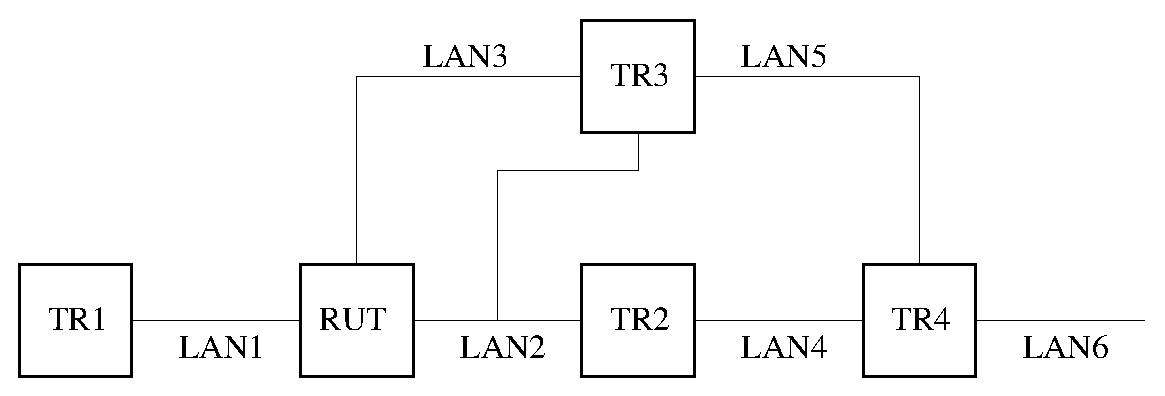
\includegraphics[scale=0.8]{figs/pim_test_6_3_sending_candidate_rp_advertisements}
    \caption{Sending Candidate-RP-Advertisements test setup}
    \label{fig:pim_test_6_3_sending_candidate_rp_advertisements}
  \end{center}
\end{figure}

\para{Procedure:}

\subpara{Part A: Periodic transmission of C-RP-Advs.}

\begin{enumerate}

  \item Start the RUT and TR1, and start observing the Cand-RP-Adv messages
  transmitted on LAN1.

  \item Compose a Bootstrap message at TR1 with the BSR address set to TR1,
  BSR priority of 10, and send it on LAN1.

  \item Continue observing the Cand-RP-Adv messages transmitted on LAN1
  for 2 * \verb=C-RP-Adv_Period= (2 * {\PimsmCRPAdvPeriod}).

\end{enumerate}

\subpara{Part B: Transmission of C-RP-Advs after the BSR changes.}

\begin{enumerate}

  \item Start the RUT, TR1, and TR2, and start observing the Cand-RP-Adv
  messages transmitted on LAN1 and LAN2.

  \item Compose a Bootstrap message at TR1 with the BSR address set to TR1,
  BSR priority of 10, and send it on LAN1.

  \item Continue observing the Cand-RP-Adv messages transmitted on LAN1
  and LAN2 for \verb=C-RP-Adv_Period= ({\PimsmCRPAdvPeriod}).

  \item Compose a Bootstrap message at TR2 with the BSR address set to TR2,
  BSR priority of 20, and send it on LAN2.

  \item Continue observing the Cand-RP-Adv messages transmitted on LAN1
  and LAN2 for 2 * \verb=C-RP-Adv_Period= (2 * {\PimsmCRPAdvPeriod}).

  \item Stop TR1 and TR2.

  \item Continue observing the Cand-RP-Adv messages transmitted on LAN1
  and LAN2 for 2 * \verb=C-RP-Adv_Period= (2 * {\PimsmCRPAdvPeriod}).

\end{enumerate}

\subpara{Part C: Transmission of C-RP-Advs when the router is a Zone Border
Router.}

\begin{enumerate}

  \item Configure the RUT such that it is a Zone Border Router for 226.0.0.0/8
  on the interface that connects the RUT to LAN2.

  \item Start the RUT and TR1, and start observing the Cand-RP-Adv messages
  transmitted on LAN1.

  \item Compose a Bootstrap message at TR1 with the BSR address set to TR1,
  BSR priority of 10, and send it on LAN1.

  \item Continue observing the Cand-RP-Adv messages transmitted on LAN1
  and LAN2 for 2 * \verb=C-RP-Adv_Period= (2 * {\PimsmCRPAdvPeriod}).

\end{enumerate}

\subpara{Part D: Transmission of C-RP-Advs when the router is gracefully shut
down.}

\begin{enumerate}

  \item Start the RUT and TR1, and start observing the Cand-RP-Adv messages
  transmitted on LAN1.

  \item Compose a Bootstrap message at TR1 with the BSR address set to TR1,
  BSR priority of 10, and send it on LAN1.

  \item Continue observing the Cand-RP-Adv messages transmitted on LAN1
  for 2 * \verb=C-RP-Adv_Period= (2 * {\PimsmCRPAdvPeriod}).

  \item Gracefully shut down the RUT.

  \item Continue observing the Cand-RP-Adv messages transmitted on LAN1
  for 2 * \verb=C-RP-Adv_Period= (2 * {\PimsmCRPAdvPeriod}).

\end{enumerate}

\para{Observable Results:}

\subpara{Part A:}

\begin{itemize}

  \item Right after the RUT receives the Bootstrap message, it should
  unicast a Cand-RP-Adv message to TR1. This message should have Prefix Count
  of 1, Priority of 192, Holdtime of \verb=C-RP_Timeout= ({\PimsmCRPTimeout}),
  RP address of the RUT address, and group prefix of 226.0.0.0/8. The Admin
  Scope Zone bit in the group prefix should not be set.

  \item After that, the RUT should periodically unicast to TR1 the same
  message, once every \verb=C-RP-Adv_Period= ({\PimsmCRPAdvPeriod}).

\end{itemize}

\subpara{Part B:}

\begin{itemize}

  \item Until before TR2 transmits the Bootstrap message on LAN2, the result
  should be same as in Part A.

  \item After TR2 transmits the Bootstrap message on LAN2, the RUT should
  immediately originate the same Cand-RP-Adv message as before, but it should
  be unicast to TR2 instead of TR1.

  \item After that, the RUT should periodically unicast to TR2 the same
  message, once every \verb=C-RP-Adv_Period= ({\PimsmCRPAdvPeriod}).

  \item After both TR1 and TR2 are shut down, then after up
  to \verb=BS_Timeout= ({\PimsmBSTimeout}), the BS Timer in the RUT should
  expire. After the BS Timer in the RUT timeout, the RUT should stop
  unicast Cand-RP-Adv messages.  

\end{itemize}

\subpara{Part C:}

\begin{itemize}

  \item The result should be same as in Part A, except that the Admin Scope
  Zone bit in the group prefix for 226.0.0.0/8 inside that message should be
  set to one.

\end{itemize}

\subpara{Part D:}

\begin{itemize}

  \item Until before the RUT is shut down, the result should be same as in
  Part A.

  \item After the RUT is shut down, it should immediately unicast the
  same Cand-RP-Adv message to TR1, except that the Holdtime inside that
  message should be set to zero.

\end{itemize}

\para{Possible Problems:}
In Part A, B, and C, the period of periodic transmission of the Cand-RP-Adv
messages might be different from \verb=C-RP-Adv_Period=
({\PimsmCRPAdvPeriod}), though it must be smaller than
\verb=C-RP_Timeout= ({\PimsmCRPTimeout}).


%%%%%%%%%%%%%%%%%%%%%%%%%%%%%%%%%%%%%%%%%%%
\newpage
\section{Creating the RP-Set at the BSR}

\para{Purpose:}
Test that the BSR creates properly the RP-Set from the
Candidate-RP-Advertisement messages (C-RP-Advs) it receives from the
Candidate-RPs.


\para{References:}
\begin{itemize}
  \item draft-ietf-pim-sm-bsr-03 -- Section 3.2
\end{itemize}

\para{Discussion:}
Upon receiving a C-RP-Adv, if the router is the BSR, then it adds the RP
address to its local pool of candidate RPs. The BSR uses the pool of C-RPs to
construct the RP-Set which is included in the Bootstrap messages and sent to
all the routers in the PIM domain.

\para{Test Setup:}
Connect the RUT, TR1, TR2, TR3, and TR4 according to
Figure~\ref{fig:pim_test_6_4_creating_the_rp_set_at_the_bsr}.
Enable PIM-SM on the RUT, TR1, TR2, TR3, and TR4. Configure the RUT
as a Cand-BSR for non-scoped zone 224.0.0.0/4 with default BSR
priority of 1, unless stated otherwise.
Configure TR1 as a Candidate-RP for 226.0.0.0/8, Candidate-RP Priority
of 192, and Holdtime of \verb=C-RP_Timeout= ({\PimsmCRPTimeout}), unless stated
otherwise.


\begin{figure}[htbp]
  \begin{center}
    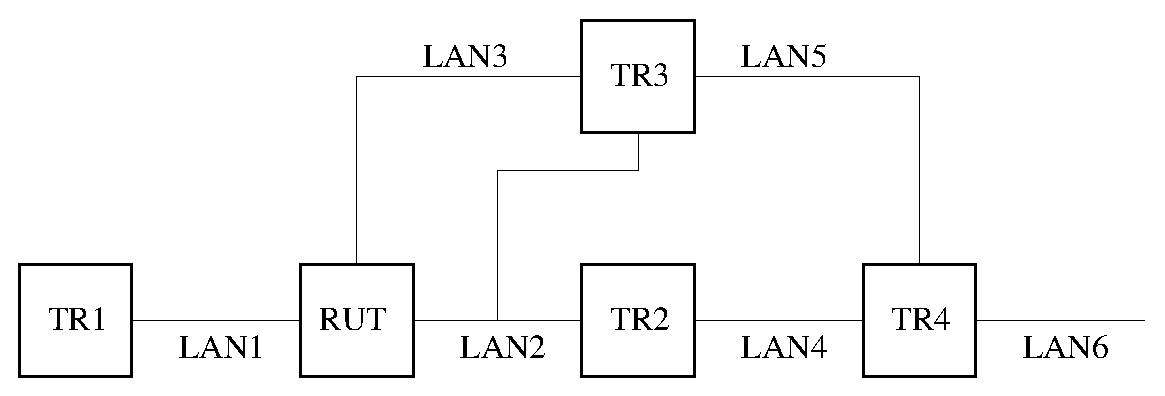
\includegraphics[scale=0.8]{figs/pim_test_6_4_creating_the_rp_set_at_the_bsr}
    \caption{Creating the RP-Set at the BSR test setup}
    \label{fig:pim_test_6_4_creating_the_rp_set_at_the_bsr}
  \end{center}
\end{figure}

\para{Procedure:}

\subpara{Part A: Receiving C-RP-Adv at non-BSR when the router is not a
cand-BSR.}

\begin{enumerate}

  \item Disable the Cand-BSR configuration in the RUT.

  \item Start the RUT and TR1, and start observing the Bootstrap messages
  transmitted on LAN1.

  \item Check the BSR and the Cand-RP state in the RUT, and the Bootstrap
  messages transmitted on LAN1.

  \item Compose a Cand-RP-Adv message at TR1 composed of TR1 as a
   Candidate-RP for 226.0.0.0/8, Candidate-RP Priority of 192, and Holdtime of
   \verb=C-RP_Timeout= ({\PimsmCRPTimeout}), and unicast it to the RUT.

  \item Check the BSR and the Cand-RP state in the RUT, and the Bootstrap
  messages transmitted on LAN1.

  \item Compose a Bootstrap message at TR1 with the BSR address set to TR1,
  BSR priority of 10, and send it on LAN1.

  \item Compose the same Cand-RP-Adv message at TR1 as before, and unicast it
  to the RUT.

  \item Check the BSR and the Cand-RP state in the RUT, and the Bootstrap
  messages transmitted on LAN1.

\end{enumerate}

\subpara{Part B: Receiving C-RP-Adv at non-BSR when the router is a cand-BSR.}

The setup is same as in Part A, except that the Cand-BSR configuration in the
RUT is not disabled.

\subpara{Part C: Receiving C-RP-Adv at the BSR.}

\begin{enumerate}

  \item Start the RUT and TR1, and start observing the Bootstrap messages
  transmitted on LAN1.

  \item Wait for up to \verb=BS_Timeout= ({\PimsmBSTimeout}) until the BS
  Timer in the RUT expires, and the RUT becomes the elected BSR.

  \item Check the BSR and the Cand-RP state in the RUT, and the Bootstrap
  messages transmitted on LAN1.

  \item Compose a Cand-RP-Adv message at TR1 composed of TR1 as a
   Candidate-RP for 226.0.0.0/8, Candidate-RP Priority of 192, and Holdtime of
   \verb=C-RP_Timeout= ({\PimsmCRPTimeout}), and unicast it to the RUT.

  \item Check the Cand-RP state in the RUT, and the Bootstrap
  messages transmitted on LAN1.

  \item Wait for up to \verb=BS_Period= ({\PimsmBSPeriod}) until the BS
  Timer in the RUT expires, and the RUT transmits another Bootstrap message on
  LAN1.

  \item Check the Cand-RP state in the RUT, and the Bootstrap
  messages transmitted on LAN1.

  \item Compose a second Cand-RP-Adv message at TR1 composed of TR1 as a
   Candidate-RP for 226.0.0.0/8, Candidate-RP Priority of 192, and Holdtime of
   \verb=C-RP_Timeout= ({\PimsmCRPTimeout}), and unicast it to the RUT.

  \item Check the Cand-RP state in the RUT, and the Bootstrap
  messages transmitted on LAN1.

  \item Compose a third Cand-RP-Adv message at TR1 composed of TR1 as a
   Candidate-RP for 226.0.0.0/8, Candidate-RP Priority of 100, and Holdtime of
   \verb=C-RP_Timeout= ({\PimsmCRPTimeout}), and unicast it to the RUT.

  \item Check the Cand-RP state in the RUT, and the Bootstrap
  messages transmitted on LAN1.

  \item Compose a fourth Cand-RP-Adv message at TR1 composed of TR1 as a
   Candidate-RP for 226.0.0.0/8, Candidate-RP Priority of 100, and Holdtime of
   0, and unicast it to the RUT.

  \item Check the Cand-RP state in the RUT, and the Bootstrap
  messages transmitted on LAN1.

  \item Compose a fifth Cand-RP-Adv message at TR1 composed of TR1 as a
   Candidate-RP for 226.0.0.0/8, Candidate-RP Priority of 192, and Holdtime of
   \verb=C-RP_Timeout= ({\PimsmCRPTimeout}), and unicast it to the RUT.

  \item Check the Cand-RP state in the RUT, and the Bootstrap
  messages transmitted on LAN1.

  \item Compose a sixth Cand-RP-Adv message at TR1 composed of TR1 as a
   Candidate-RP for 227.0.0.0/8, Candidate-RP Priority of 192, and Holdtime of
   \verb=C-RP_Timeout= ({\PimsmCRPTimeout}), and unicast it to the RUT.

  \item Check the Cand-RP state in the RUT, and the Bootstrap
  messages transmitted on LAN1.

\end{enumerate}

\subpara{Part D: Expiring C-RP at the BSR.}

\begin{enumerate}

  \item Start the RUT and TR1, and start observing the Bootstrap messages
  transmitted on LAN1.

  \item Wait for up to \verb=BS_Timeout= ({\PimsmBSTimeout}) until the BS
  Timer in the RUT expires, and the RUT becomes the elected BSR.

  \item Check the BSR and the Cand-RP state in the RUT, and the Bootstrap
  messages transmitted on LAN1.

  \item Compose a Cand-RP-Adv message at TR1 composed of TR1 as a
   Candidate-RP for 226.0.0.0/8, Candidate-RP Priority of 192, and Holdtime of
   \verb=C-RP_Timeout= ({\PimsmCRPTimeout}), and unicast it to the RUT.

  \item Check the Cand-RP state in the RUT, and the Bootstrap
  messages transmitted on LAN1.

  \item Wait for up to \verb=C-RP_Timeout= ({\PimsmCRPTimeout}) until
  the Expiry Timer of TR1's Cand-RP state in the RUT expires.

  \item Check the Cand-RP state in the RUT, and the Bootstrap
  messages transmitted on LAN1.

  \item Continue observing the Bootstrap messages transmitted on LAN1
  for at least \verb=BS_Timeout= ({\PimsmBSTimeout}).

\end{enumerate}

\subpara{Part E: Transmission of the RP-Set when the BSR is gracefully shut
down.}

\begin{enumerate}

  \item Start the RUT and TR1, and start observing the Bootstrap messages
  transmitted on LAN1.

  \item Wait for up to \verb=BS_Timeout= ({\PimsmBSTimeout}) until the BS
  Timer in the RUT expires, and the RUT becomes the elected BSR.

  \item Check the BSR and the Cand-RP state in the RUT, and the Bootstrap
  messages transmitted on LAN1.

  \item Compose a Cand-RP-Adv message at TR1 composed of TR1 as a
   Candidate-RP for 226.0.0.0/8, Candidate-RP Priority of 192, and Holdtime of
   \verb=C-RP_Timeout= ({\PimsmCRPTimeout}), and unicast it to the RUT.

  \item Check the Cand-RP state in the RUT, and the Bootstrap
  messages transmitted on LAN1.

  \item Gracefully shut down the RUT.

  \item Check the BSR and the Cand-RP state in the RUT, and the Bootstrap
  messages transmitted on LAN1.

\end{enumerate}

\para{Observable Results:}

\subpara{Part A:}

\begin{itemize}

  \item Right after the RUT is started, its BSR state machine should be in
  No Info state:

\begin{verbatim}
Xorp> show pim bootstrap 
Active zones:
BSR              Pri LocalAddress     Pri State            Timeout SZTimeout
Expiring zones:
BSR              Pri LocalAddress     Pri State            Timeout SZTimeout
Configured zones:
BSR              Pri LocalAddress     Pri State            Timeout SZTimeout
\end{verbatim}

  In addition, its RP-Set should be empty:

\begin{verbatim}
Xorp> show pim bootstrap rps 
Active RPs:
RP               Pri Timeout GroupPrefix        BSR         CandRpAdvTimeout
Expiring RPs:
RP               Pri Timeout GroupPrefix        BSR         CandRpAdvTimeout
Configured RPs:
RP               Pri Timeout GroupPrefix        BSR         CandRpAdvTimeout
\end{verbatim}

  \item When the RUT receives the first Cand-RP-Adv message, it should
  silently ignore it. In addition, its BSR state machine and its RP-Set should
  not change.

  \item After the RUT receives the Bootstrap message, it should forward it
        back on LAN1. Its BSR state machine
        should be in Accept Preferred state, and the elected BSR should be TR1.
        The BS Timer in the RUT should be set to \verb=BS_Timeout=
        ({\PimsmBSTimeout}).
        The SZ Timer in the RUT should be set to \verb=SZ_Timeout=
        ({\PimsmSZTimeout}):

\begin{verbatim}
Xorp> show pim bootstrap 
Active zones:
BSR              Pri LocalAddress     Pri State            Timeout SZTimeout
10.6.0.1          10 0.0.0.0            0 AcceptPreferred      129      1299
Expiring zones:
BSR              Pri LocalAddress     Pri State            Timeout SZTimeout
Configured zones:
BSR              Pri LocalAddress     Pri State            Timeout SZTimeout
\end{verbatim}

  However, the RP-Set should continue to be empty.

  \item When the RUT receives the second Cand-RP-Adv message, it should
  silently ignore it. In addition, its BSR state machine and its RP-Set should
  not change.

\end{itemize}

\subpara{Part B:}

\begin{itemize}

  \item Right after the RUT is started, its BSR state machine should be in
  Pending state:

\begin{verbatim}
Xorp> show pim bootstrap 
Active zones:
BSR              Pri LocalAddress     Pri State            Timeout SZTimeout
0.0.0.0            0 10.2.0.1           1 Pending               78        -1
Expiring zones:
BSR              Pri LocalAddress     Pri State            Timeout SZTimeout
Configured zones:
BSR              Pri LocalAddress     Pri State            Timeout SZTimeout
10.2.0.1           1 10.2.0.1           1 Init                  -1        -1
\end{verbatim}

  In addition, its RP-Set should be empty:

\begin{verbatim}
Xorp> show pim bootstrap rps 
Active RPs:
RP               Pri Timeout GroupPrefix        BSR         CandRpAdvTimeout
Expiring RPs:
RP               Pri Timeout GroupPrefix        BSR         CandRpAdvTimeout
Configured RPs:
RP               Pri Timeout GroupPrefix        BSR         CandRpAdvTimeout
\end{verbatim}

  \item When the RUT receives the first Cand-RP-Adv message, it should
  silently ignore it. In addition, its BSR state machine and its RP-Set should
  not change.

  \item After the RUT receives the Bootstrap message, it should forward it
        back on LAN1. Its BSR state machine
        should be in Candidate state, and the elected BSR should be TR1.
        The BS Timer in the RUT should be set to \verb=BS_Timeout=
        ({\PimsmBSTimeout}).
        The SZ Timer in the RUT should be set to \verb=SZ_Timeout=
        ({\PimsmSZTimeout}):

\begin{verbatim}
Xorp> show pim bootstrap 
Active zones:
BSR              Pri LocalAddress     Pri State            Timeout SZTimeout
10.6.0.1          10 10.2.0.1           1 Candidate            128        -1
Expiring zones:
BSR              Pri LocalAddress     Pri State            Timeout SZTimeout
Configured zones:
BSR              Pri LocalAddress     Pri State            Timeout SZTimeout
10.2.0.1           1 10.2.0.1           1 Init                  -1        -1
\end{verbatim}

  However, the RP-Set should continue to be empty.

  \item When the RUT receives the second Cand-RP-Adv message, it should
  silently ignore it. In addition, its BSR state machine and its RP-Set should
  not change.

\end{itemize}

\subpara{Part C:}

\begin{itemize}

  \item Until before the first Cand-RP-Adv message is received by the RUT, the
  RUT should be the elected BSR:

\begin{verbatim}
Xorp> show pim bootstrap 
Active zones:
BSR              Pri LocalAddress     Pri State            Timeout SZTimeout
10.2.0.1           1 10.2.0.1           1 Elected               59        -1
Expiring zones:
BSR              Pri LocalAddress     Pri State            Timeout SZTimeout
Configured zones:
BSR              Pri LocalAddress     Pri State            Timeout SZTimeout
10.2.0.1           1 10.2.0.1           1 Init                  -1        -1
\end{verbatim}

  In addition, the RP-Set in the RUT should be empty:

\begin{verbatim}
Xorp> show pim bootstrap rps 
Active RPs:
RP               Pri Timeout GroupPrefix        BSR         CandRpAdvTimeout
Expiring RPs:
RP               Pri Timeout GroupPrefix        BSR         CandRpAdvTimeout
Configured RPs:
RP               Pri Timeout GroupPrefix        BSR         CandRpAdvTimeout
\end{verbatim}

  \item After the first Cand-RP-Adv message is received by the RUT, the RP-Set
  in the RUT should include an entry for TR1 as a C-RP for 226.0.0.0/8,
  C-RP priority of 192, and holdtime of \verb=C-RP_Timeout=
  ({\PimsmCRPTimeout}).

\begin{verbatim}
Xorp> show pim bootstrap rps 
Active RPs:
RP               Pri Timeout GroupPrefix        BSR         CandRpAdvTimeout
10.6.0.1         192     149 226.0.0.0/8        10.2.0.1                  -1
Expiring RPs:
RP               Pri Timeout GroupPrefix        BSR         CandRpAdvTimeout
Configured RPs:
RP               Pri Timeout GroupPrefix        BSR         CandRpAdvTimeout
\end{verbatim}

  In addition, the RUT should (TODO: immediately?) transmit a Bootstrap
  message on LAN1 that contains TR1 as a C-RP for 226.0.0.0/8,
  C-RP priority of 192, and holdtime of \verb=C-RP_Timeout=
  ({\PimsmCRPTimeout}).

  \item After the BS Timer in the RUT expires, and it transmits the second
  Bootstrap message on LAN1, the content of this message should be same as the
  previous Bootstrap message.

  \item After the second Cand-RP-Adv message is received by the RUT, the C-RP
  Expiry Timer for TR1 in the RUT should be updated and set to
  \verb=C-RP_Timeout= ({\PimsmCRPTimeout}). The rest of the information in the
  RP-Set should not be changed:

\begin{verbatim}
Xorp> show pim bootstrap rps 
Active RPs:
RP               Pri Timeout GroupPrefix        BSR         CandRpAdvTimeout
10.6.0.1         192     149 226.0.0.0/8        10.2.0.1                  -1
Expiring RPs:
RP               Pri Timeout GroupPrefix        BSR         CandRpAdvTimeout
Configured RPs:
RP               Pri Timeout GroupPrefix        BSR         CandRpAdvTimeout
\end{verbatim}

  However, no Bootstrap message should be transmitted.

  \item After the third Cand-RP-Adv message is received by the RUT, the RP-Set
  in the RUT should include an entry for TR1 as a C-RP for 226.0.0.0/8,
  C-RP priority of 100, and holdtime of \verb=C-RP_Timeout=
  ({\PimsmCRPTimeout}).

\begin{verbatim}
Xorp> show pim bootstrap rps 
Active RPs:
RP               Pri Timeout GroupPrefix        BSR         CandRpAdvTimeout
10.6.0.1         100     144 226.0.0.0/8        10.2.0.1                  -1
Expiring RPs:
RP               Pri Timeout GroupPrefix        BSR         CandRpAdvTimeout
Configured RPs:
RP               Pri Timeout GroupPrefix        BSR         CandRpAdvTimeout
\end{verbatim}

  In addition, the RUT should (TODO: immediately?) transmit a Bootstrap
  message on LAN1 that contains TR1 as a C-RP for 226.0.0.0/8,
  C-RP priority of 100, and holdtime of \verb=C-RP_Timeout=
  ({\PimsmCRPTimeout}).

  \item After the fourth Cand-RP-Adv message is received by the RUT, the RP-Set
  in the RUT should remove the entry for TR1 as a C-RP for 226.0.0.0/8:

\begin{verbatim}
Xorp> show pim bootstrap rps 
Active RPs:
RP               Pri Timeout GroupPrefix        BSR         CandRpAdvTimeout
Expiring RPs:
RP               Pri Timeout GroupPrefix        BSR         CandRpAdvTimeout
Configured RPs:
RP               Pri Timeout GroupPrefix        BSR         CandRpAdvTimeout
\end{verbatim}

  In addition, the RUT should (TODO: immediately?) transmit a Bootstrap
  message on LAN1 that contains empty RP-Set for 226.0.0.0/8.

  \item After the fifth Cand-RP-Adv message is received by the RUT, the RP-Set
  in the RUT should include an entry for TR1 as a C-RP for 226.0.0.0/8,
  C-RP priority of 192, and holdtime of \verb=C-RP_Timeout=
  ({\PimsmCRPTimeout}).

\begin{verbatim}
Xorp> show pim bootstrap rps 
Active RPs:
RP               Pri Timeout GroupPrefix        BSR         CandRpAdvTimeout
10.6.0.1         192     144 226.0.0.0/8        10.2.0.1                  -1
Expiring RPs:
RP               Pri Timeout GroupPrefix        BSR         CandRpAdvTimeout
Configured RPs:
RP               Pri Timeout GroupPrefix        BSR         CandRpAdvTimeout
\end{verbatim}

  In addition, the RUT should (TODO: immediately?) transmit a Bootstrap
  message on LAN1 that contains TR1 as a C-RP for 226.0.0.0/8,
  C-RP priority of 192, and holdtime of \verb=C-RP_Timeout=
  ({\PimsmCRPTimeout}).

  \item After the sixth Cand-RP-Adv message is received by the RUT, the RP-Set
  in the RUT should include a second entry for TR1 as a C-RP for 227.0.0.0/8,
  C-RP priority of 192, and holdtime of \verb=C-RP_Timeout=
  ({\PimsmCRPTimeout}).

\begin{verbatim}
Xorp> show pim bootstrap rps 
Active RPs:
RP               Pri Timeout GroupPrefix        BSR         CandRpAdvTimeout
10.6.0.1         192     130 226.0.0.0/8        10.2.0.1                  -1
10.6.0.1         192     148 227.0.0.0/8        10.2.0.1                  -1
Expiring RPs:
RP               Pri Timeout GroupPrefix        BSR         CandRpAdvTimeout
Configured RPs:
RP               Pri Timeout GroupPrefix        BSR         CandRpAdvTimeout
\end{verbatim}

  In addition, the RUT should (TODO: immediately?) transmit a Bootstrap
  message on LAN1 that contains TR1 as a C-RP for 226.0.0.0/8 and 227.0.0.0/8,
  C-RP priority of 192, and holdtime of \verb=C-RP_Timeout=
  ({\PimsmCRPTimeout}).

\end{itemize}

\subpara{Part D:}

\begin{itemize}

  \item Until after the first Cand-RP-Adv message is received by the RUT, the
  results should be same as in Part C.

  \item Until before the Expiry Timer of TR1's Cand-RP state in the RUT
  expires, the RUT should periodically transmit once every
  \verb=BS_Period= ({\PimsmBSPeriod}) a Bootstrap message on LAN1. The content
  of this message should be same as the previous Bootstrap message.

  \item After the Expiry Timer of TR1's Cand-RP state in the RUT
  expires, the RUT should periodically transmit once every
  \verb=BS_Period= {\PimsmBSPeriod} a Bootstrap message on LAN1. The content
  of this message should contain empty RP-Set for 226.0.0.0/8.

  \item After \verb=BS_Timeout= ({\PimsmBSTimeout}) of periodic Bootstrap
  messages with empty RP-Set for 226.0.0.0/8, the RUT should start send
  periodic Bootstrap messages with empty RP-Set (\ie even the empty
  226.0.0.0/8 should not be included anymore).

\end{itemize}

\subpara{Part E:}

\begin{itemize}

  \item Until after the first Cand-RP-Adv message is received by the RUT, the
  results should be same as in Part C.

  \item After the RUT is shut down, it should transmit a Bootstrap message on
  LAN1 that should be same as the previous Bootstrap message, except that the
  BSR-priority is set to 0 instead of 1.

\end{itemize}

\para{Possible Problems:}
In Part D, after TR1 is removed from the RP-Set, the RUT might transmit only
one Bootstrap message with empty RP-Set for 226.0.0.0/8, and the rest of the
Bootstrap messages may not include at all 226.0.0.0/8 in the RP-Set.


%%%%%%%%%%%%%%%%%%%%%%%%%%%%%%%%%%%%%%%%%%%
\newpage
\section{Forwarding Bootstrap Messages}

\para{Purpose:}
Test that the Bootstrap messages originated at the BSR are forwarded properly.


\para{References:}
\begin{itemize}
  \item draft-ietf-pim-sm-bsr-03 -- Section 3.3
\end{itemize}

\para{Discussion:}
Bootstrap messages originated at the BSR are forwarded hop-by-hop by
intermediate routers if they pass the Bootstrap Message Processing Check.
When a Bootstrap message is forwarded, it is forwarded out on every multicast
capable-interface except if the interface is an administrative scope boundary
for the admin scope zone indicated in the first group address in the Bootstrap
message packet.

\para{Test Setup:}
Connect the RUT, TR1, TR2, TR3, and TR4 according to
Figure~\ref{fig:pim_test_6_5_forwarding_bootstrap_messages}.
Enable PIM-SM on the RUT, TR1, TR2, TR3, and TR4.
Do NOT configure any of the routers as a Cand-BSR or a Candidate-RP,
unless stated otherwise.
Configure the MRIB in the RUT such that TR2 is the next-hop router toward
TR2's address of the interface that connects TR2 to LAN4.


\begin{figure}[htbp]
  \begin{center}
    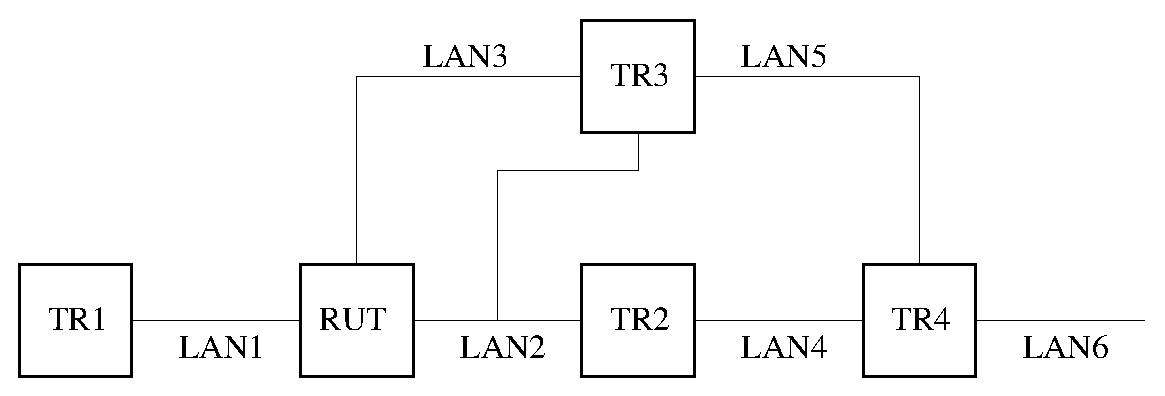
\includegraphics[scale=0.8]{figs/pim_test_6_5_forwarding_bootstrap_messages}
    \caption{Forwarding Bootstrap messages test setup}
    \label{fig:pim_test_6_5_forwarding_bootstrap_messages}
  \end{center}
\end{figure}

\para{Procedure:}

\subpara{Part A: Forwarding Bootstrap messages and scope zone boundaries.}

\begin{enumerate}

  \item Disable the interface that connects TR3 to LAN2.

  \item Start the RUT, TR1, TR2, and TR3, and start observing the Bootstrap
  messages transmitted on LAN1, LAN2, and LAN3.

  \item Compose a Bootstrap message at TR2 for scoped zone 226.0.0.0/8 with
  the BSR address set to the address of the interface that connects TR2 to
  LAN4, BSR priority of 1, Cand-RP set for 226.0.0.0/8 composed of the
  address of the interface that connects TR2 to LAN4, and send it on LAN2.

  \item Observe the Bootstrap messages transmitted on LAN1, LAN2, and LAN3.

  \item Configure the interface that connects the RUT to LAN3 as an
  administrative scope zone boundary for 226.0.0.0/8.

  \item Compose the same Bootstrap message at TR2 as before, except that the
  Fragment Tag is different, and send it on LAN2.

  \item Observe the Bootstrap messages transmitted on LAN1, LAN2, and LAN3.

  \item Gracefully stop TR1.

  \item Compose the same Bootstrap message at TR2 as before, except that the
  Fragment Tag is different, and send it on LAN2.

  \item Observe the Bootstrap messages transmitted on LAN1, LAN2, and LAN3.

\end{enumerate}

\subpara{Part B: Bootstrap message processing check.}

\begin{enumerate}

  \item Start the RUT, TR1, TR2, and TR3, and start observing the Bootstrap
  messages transmitted on LAN1, LAN2, and LAN3.

  \item Compose a Bootstrap message at TR2 for scoped zone 226.0.0.0/8 with
  the BSR address set to the address of the interface that connects TR2 to
  LAN4, BSR priority of 1, Cand-RP set for 226.0.0.0/8 composed of the
  address of the interface that connects TR2 to LAN4, and send it on LAN2.
  However, the source address of that message should be set to the address
  of the interface that connects TR2 to LAN4.

  \item Observe the Bootstrap messages transmitted on LAN1, LAN2, and LAN3.

  \item Gracefully stop TR2.

  \item Compose a Bootstrap message at TR3 for scoped zone 226.0.0.0/8 with
  the BSR address set to the address of the interface that connects TR2 to
  LAN4, BSR priority of 1, Cand-RP set for 226.0.0.0/8 composed of the
  address of the interface that connects TR2 to LAN4, and send it on LAN2.
  However, the source address of that message should be set to the address
  of the interface that connects TR2 to LAN2.

  \item Observe the Bootstrap messages transmitted on LAN1, LAN2, and LAN3.

  \item Start TR2.

  \item Compose a Bootstrap message at TR3 for scoped zone 226.0.0.0/8 with
  the BSR address set to the address of the interface that connects TR2 to
  LAN4, BSR priority of 1, Cand-RP set for 226.0.0.0/8 composed of the
  address of the interface that connects TR2 to LAN4, and send it on LAN2.

  \item Observe the Bootstrap messages transmitted on LAN1, LAN2, and LAN3.

  \item Configure the interface that connects the RUT to LAN2 as an
  administrative scope zone boundary for 226.0.0.0/8.

  \item Gracefully stop TR3.

  \item Compose a Bootstrap message at TR2 for scoped zone 226.0.0.0/8 with
  the BSR address set to the address of the interface that connects TR2 to
  LAN4, BSR priority of 1, Cand-RP set for 226.0.0.0/8 composed of the
  address of the interface that connects TR2 to LAN4, and send it on LAN2.

  \item Observe the Bootstrap messages transmitted on LAN1, LAN2, and LAN3.

  \item Remove the configuration for the administration scope zone boundary
  for 226.0.0.0/8 for the interface that connects the RUT to LAN2.

  \item Start TR3.

  \item Compose the same Bootstrap message at TR2 as before, except that the
  Fragment Tag is different, and send it on LAN2.

  \item Observe the Bootstrap messages transmitted on LAN1, LAN2, and LAN3.

  \item Compose the same Bootstrap message at TR2 as before, except that the
  Fragment Tag is different, and unicast it to the RUT.

  \item Observe the Bootstrap messages transmitted on LAN1, LAN2, and LAN3.

\end{enumerate}

\para{Observable Results:}

\subpara{Part A:}

\begin{itemize}

  \item After the RUT receives the first Bootstrap message, it should forward
  it on LAN1, LAN2, and LAN3.

  \item After the RUT receives the second Bootstrap message, it should forward
  it on LAN1 and LAN2.

  \item After the RUT receives the third Bootstrap message, it should forward
  it on LAN2.

\end{itemize}

\subpara{Part B:}

\begin{itemize}

  \item After the RUT receives the first Bootstrap message, it should silently
  ignore it.

  \item After the RUT receives the second Bootstrap message, it should silently
  ignore it.

  \item After the RUT receives the third Bootstrap message, it should silently
  ignore it.

  \item After the RUT receives the fourth Bootstrap message, it should silently
  ignore it.

  \item After the RUT receives the fifth Bootstrap message, it should forward
  it on LAN1 and LAN2.

  \item After the RUT receives the sixth Bootstrap message, it should silently
  ignore it.

\end{itemize}

\para{Possible Problems:}
None.

%%%%%%%%%%%%%%%%%%%%%%%%%%%%%%%%%%%%%%%%%%%
\newpage
\section{Receiving and Using the RP-Set}

\para{Purpose:}
Test that a router properly receives, stores, and uses a new RP-Set.


\para{References:}
\begin{itemize}
  \item draft-ietf-pim-sm-bsr-03 -- Section 3.4
\end{itemize}

\para{Discussion:}
When a router receives a new RP-Set in a Bootstrap message, it must update
properly its state. If the received RP-Set contains a new RP, the router must
add that RP to its own copy of the RP-Set. If an RP is not in the new RP-Set,
that RP is considered unreachable. After the router stores the new RP-Set, it
must recompute the RP for all existing (*,G) and (S,G,rpt) entries that might
be affected (\ie for all groups that are covered by group prefixes for which
an RP was added or deleted).

\para{Test Setup:}
Connect the RUT, TR1, TR2, TR3, and TR4 according to
Figure~\ref{fig:pim_test_6_6_receiving_and_using_the_rp_set}.
Enable PIM-SM on the RUT, TR1, TR2, TR3, and TR4.
Do NOT configure any of the routers as a Cand-BSR or a Candidate-RP,
unless stated otherwise.
Configure the MRIB in the RUT such that TR2 is the next-hop router toward
TR2's address of the interface that connects TR2 to LAN4.


\begin{figure}[htbp]
  \begin{center}
    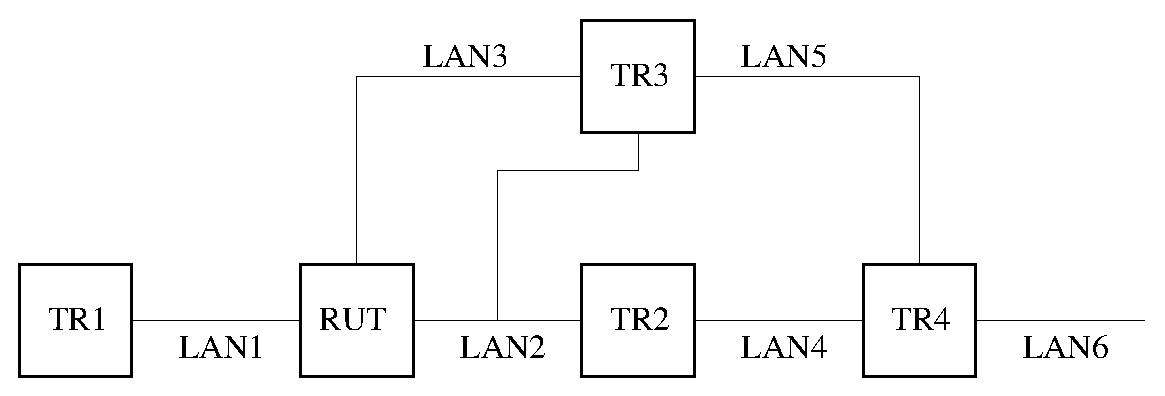
\includegraphics[scale=0.8]{figs/pim_test_6_6_receiving_and_using_the_rp_set}
    \caption{Receiving and using the RP-Set test setup}
    \label{fig:pim_test_6_6_receiving_and_using_the_rp_set}
  \end{center}
\end{figure}

\para{Procedure:}

\subpara{Part A: Receiving and using the RP-Set.}

\begin{enumerate}

  \item Start the RUT, TR1, TR2, and TR3.

  \item Start observing the RP-Set, and the (*,G) and (S,G,rpt) state in the
  RUT.

  \item Compose a Bootstrap message at TR2 with
  the BSR address set to the address of the interface that connects TR2 to
  LAN4, BSR priority of 1, Cand-RP set for 224.0.0.0/4 composed of:

  \begin{itemize}

    \item The address of the interface that connects TR2 to LAN4,
    Candidate-RP Priority of 192, and Holdtime of \verb=C-RP_Timeout=
    ({\PimsmCRPTimeout})

  \end{itemize}

  Send the Bootstrap message on LAN2.

  \item Check the RP-Set in the RUT.

  \item Compose an (*,G) Join message at TR1 with the RP address set
  to the address of the interface that connects TR2 to LAN4, and send it to
  the RUT.
  The \verb=J/P_HoldTime= of the message should be set to its default
  value ({\PimsmJPHoldTime}).

  \item Compose an (S,G,rpt) Prune message at TR1 with the source address set
  to the address of the interface that connects TR2 to LAN4, and send it to
  the RUT.
  The \verb=J/P_HoldTime= of the message should be set to its default
  value ({\PimsmJPHoldTime}).

  \item Check the (*,G) and (S,G,rpt) state in the RUT.

  \item Compose a Bootstrap message at TR2 with
  the BSR address set to the address of the interface that connects TR2 to
  LAN4, BSR priority of 1, Cand-RP set for 224.0.0.0/4 composed of:

  \begin{itemize}

    \item The address of the interface that connects TR2 to LAN4,
    Candidate-RP Priority of 192, and Holdtime of \verb=C-RP_Timeout=
    ({\PimsmCRPTimeout})

    \item The address of the interface that connects TR3 to LAN3,
    Candidate-RP Priority of 100, and Holdtime of \verb=C-RP_Timeout=
    ({\PimsmCRPTimeout})

  \end{itemize}
  The Fragment Tag of the message should be different from the previous
  Bootstrap message.
  Send the Bootstrap message on LAN2.

  \item Check the RP-Set, and the (*,G) and (S,G,rpt) state in the RUT.

  \item Compose a Bootstrap message at TR2 with
  the BSR address set to the address of the interface that connects TR2 to
  LAN4, BSR priority of 1, Cand-RP set for 224.0.0.0/4 composed of:

  \begin{itemize}

    \item The address of the interface that connects TR2 to LAN4,
    Candidate-RP Priority of 192, and Holdtime of \verb=C-RP_Timeout=
    ({\PimsmCRPTimeout})

  \end{itemize}
  The Fragment Tag of the message should be different from the previous
  Bootstrap messages.
  Send the Bootstrap message on LAN2.

  \item Check the RP-Set, and the (*,G) and (S,G,rpt) state in the RUT.

  \item Compose a Bootstrap message at TR2 with
  the BSR address set to the address of the interface that connects TR2 to
  LAN4, BSR priority of 1, Cand-RP set for 224.0.0.0/4 that has no Candidate
  RPs.
  The Fragment Tag of the message should be different from the previous
  Bootstrap messages.
  Send the Bootstrap message on LAN2.

  \item Check the RP-Set, and the (*,G) and (S,G,rpt) state in the RUT.

\end{enumerate}

\para{Observable Results:}

\subpara{Part A:}

\begin{itemize}

  \item After the RUT is started, the RP-Set in the RUT should be empty:

\begin{verbatim}
Xorp> show pim rps 
RP              Type      Pri Holdtime Timeout ActiveGroups GroupPrefix       
\end{verbatim}

  \item After the RUT receives the first Bootstrap message, the RP-Set in the
  RUT should contain TR2 only:

\begin{verbatim}
Xorp> show pim rps 
RP              Type      Pri Holdtime Timeout ActiveGroups GroupPrefix       
10.3.0.1        bootstrap 192      150     149            0 224.0.0.0/4       
\end{verbatim}

  \item After the RUT receives the (S,G,rpt) Prune message, it should contain
  (*,G) and (S,G,rpt) routing entries. The RP address for both entries should
  be set to TR2:

\begin{verbatim}
Xorp> show pim join 
Group           Source          RP              Flags
224.0.1.20      0.0.0.0         10.3.0.1        WC   
    Upstream interface (RP):   dc1
    Upstream MRIB next hop (RP): 10.2.0.2
    Upstream RPF'(*,G):        10.2.0.2
    Upstream state:            Joined 
    Join timer:                53
    Local receiver include WC: ..............
    Joins RP:                  ..............
    Joins WC:                  ........O.....
    Join state:                ........O.....
    Prune state:               ..............
    Prune pending state:       ..............
    I am assert winner state:  ..............
    I am assert loser state:   ..............
    Assert winner WC:          ..............
    Assert lost WC:            ..............
    Assert tracking WC:        .....O..O.....
    Could assert WC:           ........O.....
    I am DR:                   ........O.....
    Immediate olist RP:        ..............
    Immediate olist WC:        ........O.....
    Inherited olist SG:        ..............
    Inherited olist SG_RPT:    ..............
    PIM include WC:            ..............
224.0.1.20      10.3.0.1        10.3.0.1        SG_RPT 
    Upstream interface (S):    dc1
    Upstream interface (RP):   dc1
    Upstream MRIB next hop (RP): 10.2.0.2
    Upstream RPF'(S,G,rpt):    10.2.0.2
    Upstream state:            Pruned 
    Override timer:           -1
    Local receiver include WC: ..............
    Joins RP:                  ..............
    Joins WC:                  ........O.....
    Prunes SG_RPT:             ........O.....
    Join state:                ..............
    Prune state:               ........O.....
    Prune pending state:       ..............
    Prune tmp state:           ..............
    Prune pending tmp state:   ..............
    Assert winner WC:          ..............
    Assert lost WC:            ..............
    Assert lost SG_RPT:        ..............
    Could assert WC:           ........O.....
    Could assert SG:           ..............
    I am DR:                   ........O.....
    Immediate olist RP:        ..............
    Immediate olist WC:        ........O.....
    Inherited olist SG:        ..............
    Inherited olist SG_RPT:    ..............
    PIM include WC:            ..............
\end{verbatim}

  \item After the RUT receives the second Bootstrap message, the RP-Set in the
  RUT should contain TR2 and TR3:

\begin{verbatim}
Xorp> show pim rps 
RP              Type      Pri Holdtime Timeout ActiveGroups GroupPrefix       
10.3.0.1        bootstrap 192      150     146            0 224.0.0.0/4       
10.8.0.2        bootstrap 100      150     146            1 224.0.0.0/4       
\end{verbatim}

  In addition, the RP address for the (*,G) and (S,G,rpt) entries should be
  set to TR3:

\begin{verbatim}
Xorp> show pim join 
Group           Source          RP              Flags
224.0.1.20      0.0.0.0         10.8.0.2        WC   
    Upstream interface (RP):   dc2
    Upstream MRIB next hop (RP): 10.8.0.2
    Upstream RPF'(*,G):        10.8.0.2
    Upstream state:            Joined 
    Join timer:                54
    Local receiver include WC: ..............
    Joins RP:                  ..............
    Joins WC:                  ........O.....
    Join state:                ........O.....
    Prune state:               ..............
    Prune pending state:       ..............
    I am assert winner state:  ..............
    I am assert loser state:   ..............
    Assert winner WC:          ..............
    Assert lost WC:            ..............
    Assert tracking WC:        ......O.O.....
    Could assert WC:           ........O.....
    I am DR:                   ........O.....
    Immediate olist RP:        ..............
    Immediate olist WC:        ........O.....
    Inherited olist SG:        ..............
    Inherited olist SG_RPT:    ..............
    PIM include WC:            ..............
224.0.1.20      10.3.0.1        10.8.0.2        SG_RPT 
    Upstream interface (S):    dc1
    Upstream interface (RP):   dc2
    Upstream MRIB next hop (RP): 10.8.0.2
    Upstream RPF'(S,G,rpt):    10.8.0.2
    Upstream state:            Pruned 
    Override timer:           -1
    Local receiver include WC: ..............
    Joins RP:                  ..............
    Joins WC:                  ........O.....
    Prunes SG_RPT:             ........O.....
    Join state:                ..............
    Prune state:               ........O.....
    Prune pending state:       ..............
    Prune tmp state:           ..............
    Prune pending tmp state:   ..............
    Assert winner WC:          ..............
    Assert lost WC:            ..............
    Assert lost SG_RPT:        ..............
    Could assert WC:           ........O.....
    Could assert SG:           ..............
    I am DR:                   ........O.....
    Immediate olist RP:        ..............
    Immediate olist WC:        ........O.....
    Inherited olist SG:        ..............
    Inherited olist SG_RPT:    ..............
    PIM include WC:            ..............
\end{verbatim}

  \item After the RUT receives the third Bootstrap message, the RP-Set in the
  RUT should contain TR2 only:

\begin{verbatim}
Xorp> show pim rps 
RP              Type      Pri Holdtime Timeout ActiveGroups GroupPrefix       
10.3.0.1        bootstrap 192      150     147            1 224.0.0.0/4       
\end{verbatim}

  In addition, the RP address for the (*,G) and (S,G,rpt) entries should be
  set to TR2:

\begin{verbatim}
Xorp> show pim join 
Group           Source          RP              Flags
224.0.1.20      0.0.0.0         10.3.0.1        WC   
    Upstream interface (RP):   dc1
    Upstream MRIB next hop (RP): 10.2.0.2
    Upstream RPF'(*,G):        10.2.0.2
    Upstream state:            Joined 
    Join timer:                57
    Local receiver include WC: ..............
    Joins RP:                  ..............
    Joins WC:                  ........O.....
    Join state:                ........O.....
    Prune state:               ..............
    Prune pending state:       ..............
    I am assert winner state:  ..............
    I am assert loser state:   ..............
    Assert winner WC:          ..............
    Assert lost WC:            ..............
    Assert tracking WC:        .....O..O.....
    Could assert WC:           ........O.....
    I am DR:                   ........O.....
    Immediate olist RP:        ..............
    Immediate olist WC:        ........O.....
    Inherited olist SG:        ..............
    Inherited olist SG_RPT:    ..............
    PIM include WC:            ..............
224.0.1.20      10.3.0.1        10.3.0.1        SG_RPT 
    Upstream interface (S):    dc1
    Upstream interface (RP):   dc1
    Upstream MRIB next hop (RP): 10.2.0.2
    Upstream RPF'(S,G,rpt):    10.2.0.2
    Upstream state:            Pruned 
    Override timer:           -1
    Local receiver include WC: ..............
    Joins RP:                  ..............
    Joins WC:                  ........O.....
    Prunes SG_RPT:             ........O.....
    Join state:                ..............
    Prune state:               ........O.....
    Prune pending state:       ..............
    Prune tmp state:           ..............
    Prune pending tmp state:   ..............
    Assert winner WC:          ..............
    Assert lost WC:            ..............
    Assert lost SG_RPT:        ..............
    Could assert WC:           ........O.....
    Could assert SG:           ..............
    I am DR:                   ........O.....
    Immediate olist RP:        ..............
    Immediate olist WC:        ........O.....
    Inherited olist SG:        ..............
    Inherited olist SG_RPT:    ..............
    PIM include WC:            ..............
\end{verbatim}

  \item After the RUT receives the fourth Bootstrap message, the RP-Set in the
  RUT should be empty:

\begin{verbatim}
Xorp> show pim rps 
RP              Type      Pri Holdtime Timeout ActiveGroups GroupPrefix       
\end{verbatim}

  In addition, the RP address for the (*,G) and (S,G,rpt) entries should be
  set to UNKNOWN:

\begin{verbatim}
Xorp> show pim join 
Group           Source          RP              Flags
224.0.1.20      0.0.0.0         RP_ADDR_UNKNOWN WC   
    Upstream interface (RP):   UNKNOWN
    Upstream MRIB next hop (RP): UNKNOWN
    Upstream RPF'(*,G):        UNKNOWN
    Upstream state:            Joined 
    Join timer:                51
    Local receiver include WC: ..............
    Joins RP:                  ..............
    Joins WC:                  ........O.....
    Join state:                ........O.....
    Prune state:               ..............
    Prune pending state:       ..............
    I am assert winner state:  ..............
    I am assert loser state:   ..............
    Assert winner WC:          ..............
    Assert lost WC:            ..............
    Assert tracking WC:        ........O.....
    Could assert WC:           ........O.....
    I am DR:                   ........O.....
    Immediate olist RP:        ..............
    Immediate olist WC:        ........O.....
    Inherited olist SG:        ..............
    Inherited olist SG_RPT:    ..............
    PIM include WC:            ..............
224.0.1.20      10.3.0.1        RP_ADDR_UNKNOWN SG_RPT 
    Upstream interface (S):    dc1
    Upstream interface (RP):   UNKNOWN
    Upstream MRIB next hop (RP): UNKNOWN
    Upstream RPF'(S,G,rpt):    UNKNOWN
    Upstream state:            Pruned 
    Override timer:           -1
    Local receiver include WC: ..............
    Joins RP:                  ..............
    Joins WC:                  ........O.....
    Prunes SG_RPT:             ........O.....
    Join state:                ..............
    Prune state:               ........O.....
    Prune pending state:       ..............
    Prune tmp state:           ..............
    Prune pending tmp state:   ..............
    Assert winner WC:          ..............
    Assert lost WC:            ..............
    Assert lost SG_RPT:        ..............
    Could assert WC:           ........O.....
    Could assert SG:           ..............
    I am DR:                   ........O.....
    Immediate olist RP:        ..............
    Immediate olist WC:        ........O.....
    Inherited olist SG:        ..............
    Inherited olist SG_RPT:    ..............
    PIM include WC:            ..............
\end{verbatim}

\end{itemize}

\para{Possible Problems:}
None.

%%%%%%%%%%%%%%%%%%%%%%%%%%%%%%%%%%%%%%%%%%%
\newpage
\section{Semantic Fragmentation of BSMs}

\para{Purpose:}
Test that a router properly receives and assembles Bootstrap messages that use
semantic fragmentation.


\para{References:}
\begin{itemize}
  \item draft-ietf-pim-sm-bsr-03 -- Section 4.1.1
\end{itemize}

\para{Discussion:}
Bootstrap messages may be split over several PIM Bootstrap Message Fragment
(BSMF) packets by using semantic fragmentation.. There are two reasons for
that: (a) the BSM would exceed the link MTU the packet will be forwarded over;
and (b) the BSM includes information about more than one admin scope zone.
A router that receives BSMFs should store them and should assemble them as
more fragments are received.

\para{Test Setup:}
Connect the RUT, TR1, TR2, TR3, and TR4 according to
Figure~\ref{fig:pim_test_6_7_semantic_fragmentation_of_bsms}.
Enable PIM-SM on the RUT, TR1, TR2, TR3, and TR4.
Do NOT configure any of the routers as a Cand-BSR or a Candidate-RP,
unless stated otherwise.
Configure the MRIB in the RUT such that TR2 is the next-hop router toward
TR2's address of the interface that connects TR2 to LAN4.


\begin{figure}[htbp]
  \begin{center}
    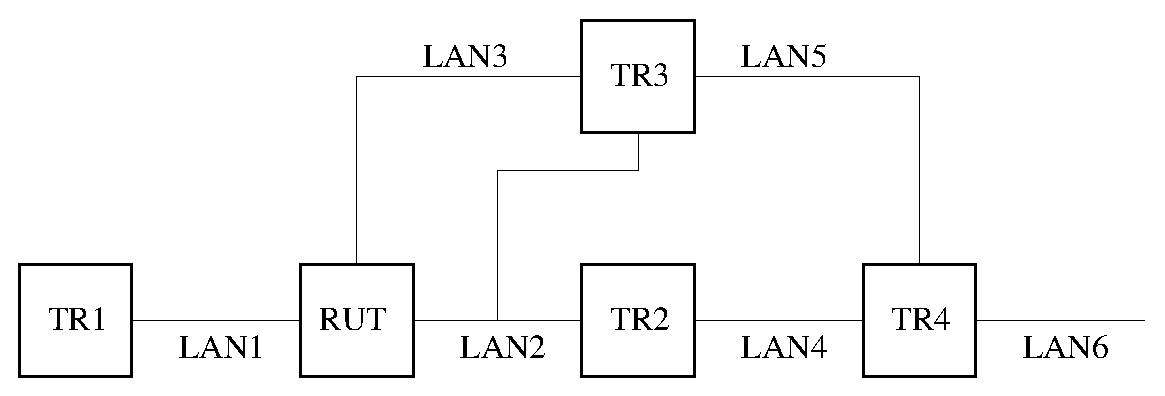
\includegraphics[scale=0.8]{figs/pim_test_6_7_semantic_fragmentation_of_bsms}
    \caption{Semantic fragmentation of BSMs test setup}
    \label{fig:pim_test_6_7_semantic_fragmentation_of_bsms}
  \end{center}
\end{figure}

\para{Procedure:}

In all scenarios, the Bootstrap message uses the following values, unless
stated otherwise:

\begin{itemize}
  \item BSR address set to TR2
  \item BSR priority set to 1
  \item Candidate-RP Priority set to 192
  \item Candidate-RP Holdtime set to \verb=C-RP_Timeout= ({\PimsmCRPTimeout})
\end{itemize}

\subpara{Part A: Split up different group prefixes in different fragments.}

\begin{enumerate}

  \item Start the RUT, TR1, and TR2.

  \item Start observing the BSR and the Cand-RP state, and the RP-Set in the
  RUT.

  \item Compose a Bootstrap message at TR2 with Cand-RP set composed of:

  \begin{itemize}

    \item Fragment Tag = 1000.

    \item Group address 1 = 224.1.0.0/16 (non-scoped),
    RP Count = 1, Frag RP Count = 1, RP Address 1 = TR1.

  \end{itemize}

  Send the Bootstrap message on LAN2.

  \item Check BSR and the Cand-RP state, and the RP-Set in the RUT.

  \item Compose a Bootstrap message at TR2 with Cand-RP set composed of:

  \begin{itemize}

    \item Fragment Tag = 1000.

    \item Group address 1 = 224.2.0.0/16 (non-scoped),
    RP Count = 1, Frag RP Count = 1, RP Address 1 = TR2.

  \end{itemize}

  Send the Bootstrap message on LAN2.

  \item Check BSR and the Cand-RP state, and the RP-Set in the RUT.

  \item Compose a Bootstrap message at TR2 with Cand-RP set composed of:

  \begin{itemize}

    \item Fragment Tag = 2000.

    \item Group address 1 = 224.1.0.0/16 (non-scoped),
    RP Count = 2, Frag RP Count = 1, RP Address 1 = TR3.

  \end{itemize}

  Send the Bootstrap message on LAN2.

  \item Check BSR and the Cand-RP state, and the RP-Set in the RUT.

  \item Compose a Bootstrap message at TR2 with Cand-RP set composed of:

  \begin{itemize}

    \item Fragment Tag = 2000.

    \item Group address 1 = 224.1.0.0/16 (non-scoped),
    RP Count = 2, Frag RP Count = 1, RP Address 1 = TR2.

  \end{itemize}

  Send the Bootstrap message on LAN2.

  \item Check BSR and the Cand-RP state, and the RP-Set in the RUT.

\end{enumerate}

\subpara{Part B: Receiving fragments for the global, non-scoped zone.}

\begin{enumerate}

  \item Start the RUT, TR1, and TR2.

  \item Start observing the BSR and the Cand-RP state, and the RP-Set in the
  RUT.

  \item Compose a Bootstrap message at TR2 with Cand-RP set composed of:

  \begin{itemize}

    \item Fragment Tag = 1000.

    \item Group address 1 = 224.0.0.0/4 (non-scoped),
    RP Count = 2, Frag RP Count = 1, RP Address 1 = TR1.

  \end{itemize}

  Send the Bootstrap message on LAN2.

  \item Check BSR and the Cand-RP state, and the RP-Set in the RUT.

  \item Compose a Bootstrap message at TR2 with Cand-RP set composed of:

  \begin{itemize}

    \item Fragment Tag = 1000.

    \item Group address 1 = 224.0.0.0/4 (non-scoped),
    RP Count = 2, Frag RP Count = 1, RP Address 1 = TR2.

  \end{itemize}

  Send the Bootstrap message on LAN2.

  \item Check BSR and the Cand-RP state, and the RP-Set in the RUT.

\end{enumerate}

\subpara{Part C: Receiving fragments for a scoped zone.}

The setup is same as in Part B, except that the RP-Set is for Group address 1
= 226.0.0.0/8 (scoped).

\subpara{Part D: Replacing the RP-Set for a group prefix.}

\begin{enumerate}

  \item Start the RUT, TR1, and TR2.

  \item Start observing the BSR and the Cand-RP state, and the RP-Set in the
  RUT.

  \item Compose a Bootstrap message at TR2 with Cand-RP set composed of:

  \begin{itemize}

    \item Fragment Tag = 1000.

    \item Group address 1 = 224.1.0.0/16 (non-scoped),
    RP Count = 1, Frag RP Count = 1, RP Address 1 = TR1.

  \end{itemize}

  Send the Bootstrap message on LAN2.

  \item Compose a Bootstrap message at TR2 with Cand-RP set composed of:

  \begin{itemize}

    \item Fragment Tag = 2000.

    \item Group address 1 = 224.1.0.0/16 (non-scoped),
    RP Count = 2, Frag RP Count = 1, RP Address 1 = TR2.

  \end{itemize}

  Send the Bootstrap message on LAN2.

  \item Check BSR and the Cand-RP state, and the RP-Set in the RUT.

  \item Compose a Bootstrap message at TR2 with Cand-RP set composed of:

  \begin{itemize}

    \item Fragment Tag = 2000.

    \item Group address 1 = 224.1.0.0/16 (non-scoped),
    RP Count = 2, Frag RP Count = 1, RP Address 1 = TR3.

  \end{itemize}

  Send the Bootstrap message on LAN2.

  \item Check BSR and the Cand-RP state, and the RP-Set in the RUT.

\end{enumerate}

\subpara{Part E: Expiring a group prefix from the RP-Set.}

\begin{enumerate}

  \item Start the RUT, TR1, and TR2.

  \item Start observing the BSR and the Cand-RP state, and the RP-Set in the
  RUT.

  \item Compose a Bootstrap message at TR2 with Cand-RP set composed of:

  \begin{itemize}

    \item Fragment Tag = 1000.

    \item Group address 1 = 224.1.1.0/24 (non-scoped),
    RP Count = 1, Frag RP Count = 1, RP Address 1 = TR1.

  \end{itemize}

  Send the Bootstrap message on LAN2.

  \item Compose a Bootstrap message at TR2 with Cand-RP set composed of:

  \begin{itemize}

    \item Fragment Tag = 2000.

    \item Group address 1 = 224.1.0.0/16 (non-scoped),
    RP Count = 2, Frag RP Count = 1, RP Address 1 = TR2.

  \end{itemize}

  Send the Bootstrap message on LAN2.

  \item Check BSR and the Cand-RP state, and the RP-Set in the RUT.

  \item Compose a Bootstrap message at TR2 with Cand-RP set composed of:

  \begin{itemize}

    \item Fragment Tag = 2000.

    \item Group address 1 = 224.1.0.0/16 (non-scoped),
    RP Count = 2, Frag RP Count = 1, RP Address 1 = TR3.

  \end{itemize}

  Send the Bootstrap message on LAN2.

  \item Check BSR and the Cand-RP state, and the RP-Set in the RUT.

  \item Continue observing the BSR and the Cand-RP state, and the RP-Set in
  the RUT for up to \verb=BS_Timeout= ({\PimsmBSTimeout}).

\end{enumerate}

\subpara{Part F: Removing a group prefix from the RP-Set.}

\begin{enumerate}

  \item Start the RUT, TR1, and TR2.

  \item Start observing the BSR and the Cand-RP state, and the RP-Set in the
  RUT.

  \item Compose a Bootstrap message at TR2 with Cand-RP set composed of:

  \begin{itemize}

    \item Fragment Tag = 1000.

    \item Group address 1 = 224.1.1.0/24 (non-scoped),
    RP Count = 1, Frag RP Count = 1, RP Address 1 = TR1.

  \end{itemize}

  Send the Bootstrap message on LAN2.

  \item Compose a Bootstrap message at TR2 with Cand-RP set composed of:

  \begin{itemize}

    \item Fragment Tag = 2000.

    \item Group address 1 = 224.1.0.0/16 (non-scoped),
    RP Count = 2, Frag RP Count = 1, RP Address 1 = TR2.

  \end{itemize}

  Send the Bootstrap message on LAN2.

  \item Check BSR and the Cand-RP state, and the RP-Set in the RUT.

  \item Compose a Bootstrap message at TR2 with Cand-RP set composed of:

  \begin{itemize}

    \item Fragment Tag = 2000.

    \item Group address 1 = 224.1.0.0/16 (non-scoped),
    RP Count = 2, Frag RP Count = 1, RP Address 1 = TR3.

  \end{itemize}

  Send the Bootstrap message on LAN2.

  \item Check BSR and the Cand-RP state, and the RP-Set in the RUT.

  \item Compose a Bootstrap message at TR2 with Cand-RP set composed of:

  \begin{itemize}

    \item Fragment Tag = 2000.

    \item Group address 1 = 224.1.1.0/24 (non-scoped),
    RP Count = 0, Frag RP Count = 0.

  \end{itemize}

  Send the Bootstrap message on LAN2.

  \item Continue observing the BSR and the Cand-RP state, and the RP-Set in
  the RUT for up to \verb=BS_Timeout= ({\PimsmBSTimeout}).

\end{enumerate}

\para{Observable Results:}

\subpara{Part A:}

\begin{itemize}

  \item After the RUT is started, the BSR state and the Cand-RP state for the
 (non-scoped) 224.0.0.0/4 zone, and the RP-Set in the RUT should be empty:

\begin{verbatim}
Xorp> show pim bootstrap 224.0.0.0/4
Active zones:
BSR              Pri LocalAddress     Pri State            Timeout SZTimeout
Expiring zones:
BSR              Pri LocalAddress     Pri State            Timeout SZTimeout
Configured zones:
BSR              Pri LocalAddress     Pri State            Timeout SZTimeout
Xorp> show pim bootstrap rps 224.0.0.0/4
Active RPs:
RP               Pri Timeout GroupPrefix        BSR         CandRpAdvTimeout
Expiring RPs:
RP               Pri Timeout GroupPrefix        BSR         CandRpAdvTimeout
Configured RPs:
RP               Pri Timeout GroupPrefix        BSR         CandRpAdvTimeout
Xorp> show pim rps 
RP              Type      Pri Holdtime Timeout ActiveGroups GroupPrefix       
\end{verbatim}

  \item After the RUT receives the first Bootstrap message, the BSR state for
  the (non-scoped) 224.0.0.0/4 zone should contain an active zone entry with
  TR2 as the BSR:

\begin{verbatim}
Xorp> show pim bootstrap 224.0.0.0/4
Active zones:
BSR              Pri LocalAddress     Pri State            Timeout SZTimeout
10.3.0.1           1 0.0.0.0            0 AcceptPreferred      123      1293
Expiring zones:
BSR              Pri LocalAddress     Pri State            Timeout SZTimeout
Configured zones:
BSR              Pri LocalAddress     Pri State            Timeout SZTimeout
\end{verbatim}

  The Cand-RP state for the (non-scoped) 224.0.0.0/4 zone should contain TR1
  for group prefix 224.1.0.0/16:

\begin{verbatim}
Xorp> show pim bootstrap rps 224.0.0.0/4
Active RPs:
RP               Pri Timeout GroupPrefix        BSR         CandRpAdvTimeout
10.6.0.1         192     139 224.1.0.0/16       10.3.0.1                  -1
Expiring RPs:
RP               Pri Timeout GroupPrefix        BSR         CandRpAdvTimeout
Configured RPs:
RP               Pri Timeout GroupPrefix        BSR         CandRpAdvTimeout
\end{verbatim}

  The RP-Set should contain TR1:

\begin{verbatim}
Xorp> show pim rps 
RP              Type      Pri Holdtime Timeout ActiveGroups GroupPrefix       
10.6.0.1        bootstrap 192      150     136            0 224.1.0.0/16      
\end{verbatim}

  \item After the RUT receives the second Bootstrap message, the BSR state for
  the (non-scoped) 224.0.0.0/4 zone should contain an active zone entry with
  TR2 as the BSR:

\begin{verbatim}
Xorp> show pim bootstrap 224.0.0.0/4
Active zones:
BSR              Pri LocalAddress     Pri State            Timeout SZTimeout
10.3.0.1           1 0.0.0.0            0 AcceptPreferred      127      1297
Expiring zones:
BSR              Pri LocalAddress     Pri State            Timeout SZTimeout
Configured zones:
BSR              Pri LocalAddress     Pri State            Timeout SZTimeout
\end{verbatim}

  The Cand-RP state for the (non-scoped) 224.0.0.0/4 zone should contain TR1
  for group prefix 224.1.0.0/16, and TR2 for group prefix  224.2.0.0/16:

\begin{verbatim}
Xorp> show pim bootstrap rps 224.0.0.0/4
Active RPs:
RP               Pri Timeout GroupPrefix        BSR         CandRpAdvTimeout
10.6.0.1         192     121 224.1.0.0/16       10.3.0.1                  -1
10.3.0.1         192     146 224.2.0.0/16       10.3.0.1                  -1
Expiring RPs:
RP               Pri Timeout GroupPrefix        BSR         CandRpAdvTimeout
Configured RPs:
RP               Pri Timeout GroupPrefix        BSR         CandRpAdvTimeout
\end{verbatim}

  The RP-Set should contain TR1 and TR2:

\begin{verbatim}
Xorp> show pim rps 
RP              Type      Pri Holdtime Timeout ActiveGroups GroupPrefix       
10.6.0.1        bootstrap 192      150     119            0 224.1.0.0/16      
10.3.0.1        bootstrap 192      150     145            0 224.2.0.0/16      
\end{verbatim}

\end{itemize}

\subpara{Part B:}

\begin{itemize}

  \item After the RUT is started, the BSR state and the Cand-RP state for the
 (non-scoped) 224.0.0.0/4 zone, and the RP-Set in the RUT should be empty:

\begin{verbatim}
Xorp> show pim bootstrap 224.0.0.0/4
Active zones:
BSR              Pri LocalAddress     Pri State            Timeout SZTimeout
Expiring zones:
BSR              Pri LocalAddress     Pri State            Timeout SZTimeout
Configured zones:
BSR              Pri LocalAddress     Pri State            Timeout SZTimeout
Xorp> show pim bootstrap rps 224.0.0.0/4
Active RPs:
RP               Pri Timeout GroupPrefix        BSR         CandRpAdvTimeout
Expiring RPs:
RP               Pri Timeout GroupPrefix        BSR         CandRpAdvTimeout
Configured RPs:
RP               Pri Timeout GroupPrefix        BSR         CandRpAdvTimeout
Xorp> show pim rps 
RP              Type      Pri Holdtime Timeout ActiveGroups GroupPrefix       
\end{verbatim}

  \item After the RUT receives the first Bootstrap message, the BSR state for
  the (non-scoped) 224.0.0.0/4 zone should contain an active zone entry with
  TR2 as the BSR:

\begin{verbatim}
Xorp> show pim bootstrap 224.0.0.0/4
Active zones:
BSR              Pri LocalAddress     Pri State            Timeout SZTimeout
10.3.0.1           1 0.0.0.0            0 AcceptPreferred      128      1298
Expiring zones:
BSR              Pri LocalAddress     Pri State            Timeout SZTimeout
Configured zones:
BSR              Pri LocalAddress     Pri State            Timeout SZTimeout
\end{verbatim}

  The Cand-RP state for the (non-scoped) 224.0.0.0/4 zone should contain TR1:

\begin{verbatim}
Xorp> show pim bootstrap rps 224.0.0.0/4
Active RPs:
RP               Pri Timeout GroupPrefix        BSR         CandRpAdvTimeout
10.6.0.1         192     147 224.0.0.0/4        10.3.0.1                  -1
Expiring RPs:
RP               Pri Timeout GroupPrefix        BSR         CandRpAdvTimeout
Configured RPs:
RP               Pri Timeout GroupPrefix        BSR         CandRpAdvTimeout
\end{verbatim}

  The RP-Set should be empty:

\begin{verbatim}
Xorp> show pim rps 
RP              Type      Pri Holdtime Timeout ActiveGroups GroupPrefix       
\end{verbatim}

  \item After the RUT receives the second Bootstrap message, the BSR state for
  the (non-scoped) 224.0.0.0/4 zone should contain an active zone entry with
  TR2 as the BSR:

\begin{verbatim}
Xorp> show pim bootstrap 224.0.0.0/4
Active zones:
BSR              Pri LocalAddress     Pri State            Timeout SZTimeout
10.3.0.1           1 0.0.0.0            0 AcceptPreferred      128      1298
Expiring zones:
BSR              Pri LocalAddress     Pri State            Timeout SZTimeout
Configured zones:
BSR              Pri LocalAddress     Pri State            Timeout SZTimeout
\end{verbatim}

  The Cand-RP state for the (non-scoped) 224.0.0.0/4 zone should contain TR1
  and TR2:

\begin{verbatim}
Xorp> show pim bootstrap rps 224.0.0.0/4
Active RPs:
RP               Pri Timeout GroupPrefix        BSR         CandRpAdvTimeout
10.6.0.1         192     132 224.0.0.0/4        10.3.0.1                  -1
10.3.0.1         192     147 224.0.0.0/4        10.3.0.1                  -1
Expiring RPs:
RP               Pri Timeout GroupPrefix        BSR         CandRpAdvTimeout
Configured RPs:
RP               Pri Timeout GroupPrefix        BSR         CandRpAdvTimeout
\end{verbatim}

  The RP-Set should contain TR1 and TR2:

\begin{verbatim}
Xorp> show pim rps 
RP              Type      Pri Holdtime Timeout ActiveGroups GroupPrefix       
10.6.0.1        bootstrap 192      150     131            0 224.0.0.0/4       
10.3.0.1        bootstrap 192      150     146            0 224.0.0.0/4       
\end{verbatim}

\end{itemize}

\subpara{Part C:}

The results should be same as in Part B, except that 224.0.0.0/4 is
substituted everywhere with 226.0.0.0/8, and except that
the CLI commands to show the scoped-zone results are:
\begin{verbatim}
Xorp> show pim bootstrap 226.0.0.0/8 scoped
...
Xorp> show pim bootstrap rps 226.0.0.0/8 scoped
...
Xorp> show pim rps 
...
\end{verbatim}

\subpara{Part D:}

\begin{itemize}

  \item After the RUT is started, the BSR state and the Cand-RP state for the
 (non-scoped) 224.0.0.0/4 zone, and the RP-Set in the RUT should be empty:

\begin{verbatim}
Xorp> show pim bootstrap 224.0.0.0/4
Active zones:
BSR              Pri LocalAddress     Pri State            Timeout SZTimeout
Expiring zones:
BSR              Pri LocalAddress     Pri State            Timeout SZTimeout
Configured zones:
BSR              Pri LocalAddress     Pri State            Timeout SZTimeout
Xorp> show pim bootstrap rps 224.0.0.0/4
Active RPs:
RP               Pri Timeout GroupPrefix        BSR         CandRpAdvTimeout
Expiring RPs:
RP               Pri Timeout GroupPrefix        BSR         CandRpAdvTimeout
Configured RPs:
RP               Pri Timeout GroupPrefix        BSR         CandRpAdvTimeout
Xorp> show pim rps 
RP              Type      Pri Holdtime Timeout ActiveGroups GroupPrefix       
\end{verbatim}

  \item After the RUT receives the first Bootstrap message, the BSR state for
  the (non-scoped) 224.0.0.0/4 zone should contain an active zone entry with
  TR2 as the BSR:

\begin{verbatim}
Xorp> show pim bootstrap 224.0.0.0/4
Active zones:
BSR              Pri LocalAddress     Pri State            Timeout SZTimeout
10.3.0.1           1 0.0.0.0            0 AcceptPreferred      128      1298
Expiring zones:
BSR              Pri LocalAddress     Pri State            Timeout SZTimeout
Configured zones:
BSR              Pri LocalAddress     Pri State            Timeout SZTimeout
\end{verbatim}

  The Cand-RP state for the (non-scoped) 224.0.0.0/4 zone should contain TR1
  for group prefix 224.1.0.0/16:

\begin{verbatim}
Xorp> show pim bootstrap rps 224.0.0.0/4
Active RPs:
RP               Pri Timeout GroupPrefix        BSR         CandRpAdvTimeout
10.6.0.1         192     146 224.1.0.0/16       10.3.0.1                  -1
Expiring RPs:
RP               Pri Timeout GroupPrefix        BSR         CandRpAdvTimeout
Configured RPs:
RP               Pri Timeout GroupPrefix        BSR         CandRpAdvTimeout
\end{verbatim}

  The RP-Set should contain TR1 as an RP for group prefix 224.1.0.0/16:

\begin{verbatim}
Xorp> show pim rps 
RP              Type      Pri Holdtime Timeout ActiveGroups GroupPrefix       
10.6.0.1        bootstrap 192      150     145            0 224.1.0.0/16      
\end{verbatim}

  \item After the RUT receives the second Bootstrap message, the BSR state for
  the (non-scoped) 224.0.0.0/4 zone should contain an active zone entry with
  TR2 as the BSR, as well as an expiring zone:

\begin{verbatim}
Xorp> show pim bootstrap 224.0.0.0/4
Active zones:
BSR              Pri LocalAddress     Pri State            Timeout SZTimeout
10.3.0.1           1 0.0.0.0            0 AcceptPreferred      128      1298
Expiring zones:
BSR              Pri LocalAddress     Pri State            Timeout SZTimeout
10.3.0.1           1 0.0.0.0            0 AcceptPreferred        0        -1
Configured zones:
BSR              Pri LocalAddress     Pri State            Timeout SZTimeout
\end{verbatim}

  The Cand-RP state for the (non-scoped) 224.0.0.0/4 zone should
  contain TR2 as an active RP for group prefix 224.1.0.0/16, and TR1 as an
  expiring RP for group prefix 224.1.0.0/16:

\begin{verbatim}
Xorp> show pim bootstrap rps 224.0.0.0/4
Active RPs:
RP               Pri Timeout GroupPrefix        BSR         CandRpAdvTimeout
10.3.0.1         192     147 224.1.0.0/16       10.3.0.1                  -1
Expiring RPs:
RP               Pri Timeout GroupPrefix        BSR         CandRpAdvTimeout
10.6.0.1         192     129 224.1.0.0/16       10.3.0.1                  -1
Configured RPs:
RP               Pri Timeout GroupPrefix        BSR         CandRpAdvTimeout
\end{verbatim}

  The RP-Set should contain TR1 as an RP for group prefix 224.1.0.0/16:

\begin{verbatim}
Xorp> show pim rps 
RP              Type      Pri Holdtime Timeout ActiveGroups GroupPrefix       
10.6.0.1        bootstrap 192      150     127            0 224.1.0.0/16      
\end{verbatim}

  \item After the RUT receives the third Bootstrap message, the BSR state for
  the (non-scoped) 224.0.0.0/4 zone should contain an active zone entry with
  TR2 as the BSR:

\begin{verbatim}
Xorp> show pim bootstrap 224.0.0.0/4
Active zones:
BSR              Pri LocalAddress     Pri State            Timeout SZTimeout
10.3.0.1           1 0.0.0.0            0 AcceptPreferred      128      1298
Expiring zones:
BSR              Pri LocalAddress     Pri State            Timeout SZTimeout
Configured zones:
BSR              Pri LocalAddress     Pri State            Timeout SZTimeout
\end{verbatim}

  The Cand-RP state for the (non-scoped) 224.0.0.0/4 zone should
  contain TR2 and TR3 as active RPs for group prefix 224.1.0.0/16:

\begin{verbatim}
Xorp> show pim bootstrap rps 224.0.0.0/4
Active RPs:
RP               Pri Timeout GroupPrefix        BSR         CandRpAdvTimeout
10.3.0.1         192     131 224.1.0.0/16       10.3.0.1                  -1
10.2.0.4         192     147 224.1.0.0/16       10.3.0.1                  -1
Expiring RPs:
RP               Pri Timeout GroupPrefix        BSR         CandRpAdvTimeout
Configured RPs:
RP               Pri Timeout GroupPrefix        BSR         CandRpAdvTimeout
\end{verbatim}

  The RP-Set should contain TR2 and TR3 as RPs for group prefix 224.1.0.0/16:

\begin{verbatim}
Xorp> show pim rps 
RP              Type      Pri Holdtime Timeout ActiveGroups GroupPrefix       
10.3.0.1        bootstrap 192      150     130            0 224.1.0.0/16      
10.2.0.4        bootstrap 192      150     146            0 224.1.0.0/16      
\end{verbatim}

\end{itemize}

\subpara{Part E:}

\begin{itemize}

  \item After the RUT is started, the BSR state and the Cand-RP state for the
 (non-scoped) 224.0.0.0/4 zone, and the RP-Set in the RUT should be empty:

\begin{verbatim}
Xorp> show pim bootstrap 224.0.0.0/4
Active zones:
BSR              Pri LocalAddress     Pri State            Timeout SZTimeout
Expiring zones:
BSR              Pri LocalAddress     Pri State            Timeout SZTimeout
Configured zones:
BSR              Pri LocalAddress     Pri State            Timeout SZTimeout
Xorp> show pim bootstrap rps 224.0.0.0/4
Active RPs:
RP               Pri Timeout GroupPrefix        BSR         CandRpAdvTimeout
Expiring RPs:
RP               Pri Timeout GroupPrefix        BSR         CandRpAdvTimeout
Configured RPs:
RP               Pri Timeout GroupPrefix        BSR         CandRpAdvTimeout
Xorp> show pim rps 
RP              Type      Pri Holdtime Timeout ActiveGroups GroupPrefix       
\end{verbatim}

  \item After the RUT receives the first Bootstrap message, the BSR state for
  the (non-scoped) 224.0.0.0/4 zone should contain an active zone entry with
  TR2 as the BSR:

\begin{verbatim}
Xorp> show pim bootstrap 224.0.0.0/4
Active zones:
BSR              Pri LocalAddress     Pri State            Timeout SZTimeout
10.3.0.1           1 0.0.0.0            0 AcceptPreferred      127      1297
Expiring zones:
BSR              Pri LocalAddress     Pri State            Timeout SZTimeout
Configured zones:
BSR              Pri LocalAddress     Pri State            Timeout SZTimeout
\end{verbatim}

  The Cand-RP state for the (non-scoped) 224.0.0.0/4 zone should contain TR1
  for group prefix 224.1.1.0/24:

\begin{verbatim}
Xorp> show pim bootstrap rps 224.0.0.0/4
Active RPs:
RP               Pri Timeout GroupPrefix        BSR         CandRpAdvTimeout
10.6.0.1         192     146 224.1.1.0/24       10.3.0.1                  -1
Expiring RPs:
RP               Pri Timeout GroupPrefix        BSR         CandRpAdvTimeout
Configured RPs:
RP               Pri Timeout GroupPrefix        BSR         CandRpAdvTimeout
\end{verbatim}

  The RP-Set should contain TR1 as an RP for group prefix 224.1.1.0/24:

\begin{verbatim}
Xorp> show pim rps 
RP              Type      Pri Holdtime Timeout ActiveGroups GroupPrefix       
10.6.0.1        bootstrap 192      150     143            0 224.1.1.0/24      
\end{verbatim}

  \item After the RUT receives the second Bootstrap message, the BSR state for
  the (non-scoped) 224.0.0.0/4 zone should contain an active zone entry with
  TR2 as the BSR, as well as an expiring zone:

\begin{verbatim}
Xorp> show pim bootstrap 224.0.0.0/4
Active zones:
BSR              Pri LocalAddress     Pri State            Timeout SZTimeout
10.3.0.1           1 0.0.0.0            0 AcceptPreferred      128      1298
Expiring zones:
BSR              Pri LocalAddress     Pri State            Timeout SZTimeout
10.3.0.1           1 0.0.0.0            0 AcceptPreferred        0        -1
Configured zones:
BSR              Pri LocalAddress     Pri State            Timeout SZTimeout
\end{verbatim}

  The Cand-RP state for the (non-scoped) 224.0.0.0/4 zone should
  contain TR2 as an active RP for group prefix 224.1.0.0/16, and TR1 as an
  expiring RP for group prefix 224.1.1.0/24:

\begin{verbatim}
Xorp> show pim bootstrap rps 224.0.0.0/4
Active RPs:
RP               Pri Timeout GroupPrefix        BSR         CandRpAdvTimeout
10.3.0.1         192     147 224.1.0.0/16       10.3.0.1                  -1
Expiring RPs:
RP               Pri Timeout GroupPrefix        BSR         CandRpAdvTimeout
10.6.0.1         192     124 224.1.1.0/24       10.3.0.1                  -1
Configured RPs:
RP               Pri Timeout GroupPrefix        BSR         CandRpAdvTimeout
\end{verbatim}

  The RP-Set should contain TR1 as an RP for group prefix 224.1.0.0/16:

\begin{verbatim}
Xorp> show pim rps 
RP              Type      Pri Holdtime Timeout ActiveGroups GroupPrefix       
10.6.0.1        bootstrap 192      150     122            0 224.1.1.0/24      
\end{verbatim}

  \item After the RUT receives the third Bootstrap message, the BSR state for
  the (non-scoped) 224.0.0.0/4 zone should contain an active zone entry with
  TR2 as the BSR, as well as an expiring zone:

\begin{verbatim}
Xorp> show pim bootstrap 224.0.0.0/4
Active zones:
BSR              Pri LocalAddress     Pri State            Timeout SZTimeout
10.3.0.1           1 0.0.0.0            0 AcceptPreferred      128      1298
Expiring zones:
BSR              Pri LocalAddress     Pri State            Timeout SZTimeout
10.3.0.1           1 0.0.0.0            0 AcceptPreferred        0        -1
Configured zones:
BSR              Pri LocalAddress     Pri State            Timeout SZTimeout
\end{verbatim}

  The Cand-RP state for the (non-scoped) 224.0.0.0/4 zone should
  contain TR2 and TR3 as active RPs for group prefix 224.1.0.0/16, and TR1 as
  an expiring RP for group prefix 224.1.1.0/24:

\begin{verbatim}
Xorp> show pim bootstrap rps 224.0.0.0/4
Active RPs:
RP               Pri Timeout GroupPrefix        BSR         CandRpAdvTimeout
10.3.0.1         192     128 224.1.0.0/16       10.3.0.1                  -1
10.2.0.4         192     146 224.1.0.0/16       10.3.0.1                  -1
Expiring RPs:
RP               Pri Timeout GroupPrefix        BSR         CandRpAdvTimeout
10.6.0.1         192     106 224.1.1.0/24       10.3.0.1                  -1
Configured RPs:
RP               Pri Timeout GroupPrefix        BSR         CandRpAdvTimeout
\end{verbatim}

  The RP-Set should contain TR1 as an RP for group prefix 224.1.1.0/24, and TR2
  and TR3 as RPs for group prefix 224.1.0.0/16:

\begin{verbatim}
Xorp> show pim rps 
RP              Type      Pri Holdtime Timeout ActiveGroups GroupPrefix       
10.6.0.1        bootstrap 192      150     104            0 224.1.1.0/24      
10.3.0.1        bootstrap 192      150     126            0 224.1.0.0/16      
10.2.0.4        bootstrap 192      150     144            0 224.1.0.0/16      
\end{verbatim}

  \item After up to \verb=C-RP_Timeout= ({\PimsmCRPTimeout}) or
  \verb=BS_Timeout= ({\PimsmBSTimeout}) (whichever comes first), the
  state for group prefix 224.1.1.0/24 and Cand-RP TR1 should expire:

\begin{verbatim}
Xorp> show pim bootstrap 224.0.0.0/4
Active zones:
BSR              Pri LocalAddress     Pri State            Timeout SZTimeout
10.3.0.1           1 0.0.0.0            0 AcceptPreferred       16      1186
Expiring zones:
BSR              Pri LocalAddress     Pri State            Timeout SZTimeout
Configured zones:
BSR              Pri LocalAddress     Pri State            Timeout SZTimeout
\end{verbatim}

\begin{verbatim}
Xorp> show pim bootstrap rps 224.0.0.0/4
Active RPs:
RP               Pri Timeout GroupPrefix        BSR         CandRpAdvTimeout
10.3.0.1         192      17 224.1.0.0/16       10.3.0.1                  -1
10.2.0.4         192      34 224.1.0.0/16       10.3.0.1                  -1
Expiring RPs:
RP               Pri Timeout GroupPrefix        BSR         CandRpAdvTimeout
Configured RPs:
RP               Pri Timeout GroupPrefix        BSR         CandRpAdvTimeout
\end{verbatim}

  In addition, TR1 should be removed from the RP-Set as well:

\begin{verbatim}
Xorp> show pim rps 
RP              Type      Pri Holdtime Timeout ActiveGroups GroupPrefix       
10.3.0.1        bootstrap 192      150      15            0 224.1.0.0/16      
10.2.0.4        bootstrap 192      150      33            0 224.1.0.0/16      
\end{verbatim}

\end{itemize}

\para{Possible Problems:}
None.

\subpara{Part F:}

\begin{itemize}

  \item Until after the third Bootstrap message is transmitted, the result
  should be same as in Section E.

  \item After the RUT receives the fourth Bootstrap message, the BSR state for
  the (non-scoped) 224.0.0.0/4 zone should contain an active zone entry with
  TR2 as the BSR:

\begin{verbatim}
Xorp> show pim bootstrap 224.0.0.0/4
Active zones:
BSR              Pri LocalAddress     Pri State            Timeout SZTimeout
10.3.0.1           1 0.0.0.0            0 AcceptPreferred      128      1298
Expiring zones:
BSR              Pri LocalAddress     Pri State            Timeout SZTimeout
Configured zones:
BSR              Pri LocalAddress     Pri State            Timeout SZTimeout
\end{verbatim}

  The Cand-RP state for the (non-scoped) 224.0.0.0/4 zone should
  contain TR2 and TR3 as active RPs for group prefix 224.1.0.0/16:

\begin{verbatim}
Xorp> show pim bootstrap rps 224.0.0.0/4
Active RPs:
RP               Pri Timeout GroupPrefix        BSR         CandRpAdvTimeout
10.3.0.1         192     103 224.1.0.0/16       10.3.0.1                  -1
10.2.0.4         192     123 224.1.0.0/16       10.3.0.1                  -1
Expiring RPs:
RP               Pri Timeout GroupPrefix        BSR         CandRpAdvTimeout
Configured RPs:
RP               Pri Timeout GroupPrefix        BSR         CandRpAdvTimeout
\end{verbatim}

  The RP-Set should contain TR2 and TR3 as RPs for group prefix 224.1.0.0/16:

\begin{verbatim}
Xorp> show pim rps 
RP              Type      Pri Holdtime Timeout ActiveGroups GroupPrefix       
10.3.0.1        bootstrap 192      150     101            0 224.1.0.0/16      
10.2.0.4        bootstrap 192      150     122            0 224.1.0.0/16      
\end{verbatim}

\end{itemize}

\para{Possible Problems:}
None.

% %%%%%%%%%%%%%%%%%%%%%%%%%%%%%%%%%%%%%%%%%%%
% \newpage
% \section{Template}

% \para{Purpose:}
% TODO

% \para{References:}
% \begin{itemize}
%   \item draft-ietf-pim-sm-v2-new-05 -- Section TODO
% \end{itemize}

% \para{Discussion:}
% TODO

% \para{Test Setup:}
% TODO

% \para{Procedure:}
% TODO

% \para{Observable Results:}
% TODO

% \para{Possible Problems:}
% TODO

%%%%%%%%%%%%%%%%%%%%%%%%%%%%%%%%%%%%%%%%%%%%%%%%%%%%%%%%%%%%%%%%%%%%%%%
%     BIBLIOGRAPHY
%%%%%%%%%%%%%%%%%%%%%%%%%%%%%%%%%%%%%%%%%%%%%%%%%%%%%%%%%%%%%%%%%%%%%%%

% \bibliography{pim_testsuite}
% \bibliographystyle{plain}

%%%%%%%%%%%%%%%%%%%%%%%%%%%%%%%%%%%%%%%%%%%
\newpage

\center{\huge This is the last page.}

\end{document}

